% =============================================================================
%  main.tex —— 《无穷范畴讲义》中译注本主文件
%  编译：在 源码/ 目录下执行  xelatex main.tex  三遍
% =============================================================================
% =============================================================================
%  preamble.tex —— 中译注本《无穷范畴讲义》导言区
%  底本：Lin Chen, Lectures on Infinity Categories, 2024（27 讲，203 页）
%  编译：xelatex main.tex ×3（本文件与 main.tex 由 Lead 维护，译手不得改动）
% =============================================================================
\documentclass[UTF8, fontset=fandol, 11pt, a4paper, oneside]{ctexart}

\usepackage{amsmath}
\usepackage{amssymb}
\usepackage{amsthm}
\usepackage{mathtools}
\usepackage{bm}
\usepackage{mathrsfs}
\usepackage[a4paper,left=2.6cm,right=2.6cm,top=2.8cm,bottom=2.8cm,headsep=0.5cm,footskip=1.1cm]{geometry}
\usepackage{graphicx}
\usepackage{xcolor}
\usepackage{enumitem}
\usepackage{booktabs}
\usepackage{longtable}
\usepackage{array}
\usepackage{multirow}
\usepackage{tikz}
\usepackage{tikz-cd}
\usepackage{fancyhdr}
\usepackage{newunicodechar}
% 正文中不慎以文本模式出现的符号，自动转成数学模式
\newunicodechar{∞}{\ensuremath{\infty}}
\newunicodechar{≃}{\ensuremath{\simeq}}
\newunicodechar{→}{\ensuremath{\to}}
\newunicodechar{←}{\ensuremath{\leftarrow}}
\newunicodechar{⊗}{\ensuremath{\otimes}}
\newunicodechar{⊕}{\ensuremath{\oplus}}
\newunicodechar{×}{\ensuremath{\times}}
\newunicodechar{≅}{\ensuremath{\cong}}
\newunicodechar{≠}{\ensuremath{\neq}}
\newunicodechar{≤}{\ensuremath{\leq}}
\newunicodechar{≥}{\ensuremath{\geq}}
\newunicodechar{∈}{\ensuremath{\in}}
\newunicodechar{⊂}{\ensuremath{\subset}}
\newunicodechar{∘}{\ensuremath{\circ}}
\newunicodechar{∆}{\ensuremath{\Delta}}
\newunicodechar{Λ}{\ensuremath{\Lambda}}
\newunicodechar{∂}{\ensuremath{\partial}}
\newunicodechar{π}{\ensuremath{\pi}}
\newunicodechar{α}{\ensuremath{\alpha}}\newunicodechar{β}{\ensuremath{\beta}}
\newunicodechar{γ}{\ensuremath{\gamma}}\newunicodechar{δ}{\ensuremath{\delta}}
\newunicodechar{ε}{\ensuremath{\varepsilon}}\newunicodechar{ζ}{\ensuremath{\zeta}}
\newunicodechar{η}{\ensuremath{\eta}}\newunicodechar{θ}{\ensuremath{\theta}}
\newunicodechar{ι}{\ensuremath{\iota}}\newunicodechar{κ}{\ensuremath{\kappa}}
\newunicodechar{λ}{\ensuremath{\lambda}}\newunicodechar{μ}{\ensuremath{\mu}}
\newunicodechar{ν}{\ensuremath{\nu}}\newunicodechar{ξ}{\ensuremath{\xi}}
\newunicodechar{ρ}{\ensuremath{\rho}}\newunicodechar{σ}{\ensuremath{\sigma}}
\newunicodechar{τ}{\ensuremath{\tau}}\newunicodechar{υ}{\ensuremath{\upsilon}}
\newunicodechar{φ}{\ensuremath{\varphi}}\newunicodechar{χ}{\ensuremath{\chi}}
\newunicodechar{ψ}{\ensuremath{\psi}}\newunicodechar{ω}{\ensuremath{\omega}}
\newunicodechar{Γ}{\ensuremath{\Gamma}}\newunicodechar{Θ}{\ensuremath{\Theta}}
\newunicodechar{Ξ}{\ensuremath{\Xi}}\newunicodechar{Π}{\ensuremath{\Pi}}
\newunicodechar{Σ}{\ensuremath{\Sigma}}\newunicodechar{Φ}{\ensuremath{\Phi}}
\newunicodechar{Ψ}{\ensuremath{\Psi}}\newunicodechar{Ω}{\ensuremath{\Omega}}
\usepackage[colorlinks=true,linkcolor=blue!45!black,citecolor=blue!45!black,urlcolor=blue!45!black,bookmarksnumbered=true]{hyperref}

% ---------------------------------------------------------------------------
% 版式
% ---------------------------------------------------------------------------
\linespread{1.28}
\setlength{\emergencystretch}{3em}
\allowdisplaybreaks[3]
\setlength{\parindent}{2em}
\setlength{\parskip}{0.15em}
\setcounter{tocdepth}{1}
\setcounter{secnumdepth}{3}

\pagestyle{fancy}
\fancyhf{}
\fancyhead[L]{\small\songti 无穷范畴讲义}
\fancyhead[R]{\small\songti\leftmark}
\fancyfoot[C]{\small\thepage}
\renewcommand{\headrulewidth}{0.4pt}
\renewcommand{\footrulewidth}{0pt}

\renewcommand{\contentsname}{目\hspace{2em}录}
\renewcommand{\figurename}{图}
\renewcommand{\tablename}{表}
\renewcommand{\proofname}{证明}
\renewcommand{\appendixname}{附录}
\renewcommand{\sectionmark}[1]{}
\ctexset{
  section/format = {\Large\bfseries\centering},
  section/aftername = {.\quad},
  section/number = \arabic{section},
  subsection/format = {\large\bfseries\raggedright},
}

% ---------------------------------------------------------------------------
% 讲一级标题（不编号）
% ---------------------------------------------------------------------------
\newcounter{lecture}
\newif\iflecapp
\newcommand{\lecture}[2]{%
  \clearpage
  \stepcounter{lecture}%
  \setcounter{section}{0}%
  \setcounter{nitem}{0}%
  \setcounter{equation}{0}%
  \setcounter{footnote}{0}%
  \lecappfalse
  \renewcommand{\thesection}{\arabic{section}}%
  \renewcommand{\theHsection}{lec\thelecture.\arabic{section}}%
  \section*{第 #1 讲\quad #2}%
  \addcontentsline{toc}{section}{第 #1 讲\quad #2}%
  \markboth{第 #1 讲\quad #2}{第 #1 讲\quad #2}%
}

% 附录小节：打印“附录 A　……”，并让 nitem 编号变成 A.1
\newcommand{\appendixsection}[1]{%
  \par
  \iflecapp
    \refstepcounter{section}%
  \else
    \setcounter{section}{0}%
    \renewcommand{\thesection}{\Alph{section}}%
    \lecapptrue
    \refstepcounter{section}%
  \fi
  \setcounter{nitem}{0}%
  \renewcommand{\theHsection}{lec\thelecture.\Alph{section}}%
  \section*{附录 \thesection\quad #1}%
  \addcontentsline{toc}{section}{附录 \thesection\quad #1}%
  \markright{附录 \thesection\quad #1}%
}

% ---------------------------------------------------------------------------
% 编号：每节一个统一计数器，原书所有编号对象共用“节.序号”
% ---------------------------------------------------------------------------
\newcounter{nitem}[section]
\renewcommand{\thenitem}{\thesection.\arabic{nitem}}
\renewcommand{\theHnitem}{lec\thelecture.\thesection.\arabic{nitem}}

\newtheoremstyle{cnplain}{0.9em}{0.6em}{\normalfont}{}{\bfseries}{.}{0.5em}{}
\theoremstyle{cnplain}
\newtheorem{theorem}[nitem]{定理}
\newtheorem{proposition}[nitem]{命题}
\newtheorem{lemma}[nitem]{引理}
\newtheorem{corollary}[nitem]{推论}
\newtheorem{conjecture}[nitem]{猜想}
\newtheorem{claim}[nitem]{断言}
\newtheorem{slogan}[nitem]{口号}
\newtheorem{question}[nitem]{问题}
\theoremstyle{definition}
\newtheorem{definition}[nitem]{定义}
\newtheorem{example}[nitem]{例}
\newtheorem{exercise}[nitem]{练习}
\newtheorem{challenge}[nitem]{挑战}
\newtheorem{construction}[nitem]{构造}
\newtheorem{variant}[nitem]{变体}
\newtheorem{remark}[nitem]{注}
\newtheorem{notation}[nitem]{记号}
\newtheorem{warning}[nitem]{警告}
\newtheorem{convention}[nitem]{约定}
\newtheorem{theoremdef}[nitem]{定理—定义}

% 普通编号段落：2.1. 正文……
\newcommand{\nitem}{%
  \par\refstepcounter{nitem}%
  \noindent\hspace*{2em}\thenitem.\hspace{0.5em}\ignorespaces
}

\numberwithin{equation}{section}

% 图占位（Lead 统一重绘后替换）
\newcommand{\FIGPLACEHOLDER}[1]{\fbox{\small 图 #1（待重绘）}}

% 译注：左侧竖线小字；\showyizhufalse 可隐藏
\newif\ifshowyizhu
\showyizhutrue
\newcommand{\yizhu}[1]{\ifshowyizhu\par\smallskip\noindent{\small\color{black!72}%
  \hspace*{0.4em}\vrule width 0.8pt\hspace{0.6em}\begin{minipage}[t]{0.9\linewidth}\raggedright #1\end{minipage}}\smallskip\fi}

% ---------------------------------------------------------------------------
% 常用记号（全书统一；译手只许使用这里定义的宏，见 STYLE_GUIDE.md §3）
% ---------------------------------------------------------------------------
\newcommand{\Z}{\mathbb{Z}}
\newcommand{\Q}{\mathbb{Q}}
\newcommand{\R}{\mathbb{R}}
\newcommand{\C}{\mathbb{C}}
\newcommand{\N}{\mathbb{N}}
\newcommand{\PP}{\mathbb{P}}
\newcommand{\A}{\mathbb{A}}
\newcommand{\GG}{\mathbb{G}}
\newcommand{\OO}{\mathcal{O}}
\newcommand{\cA}{\mathcal{A}}\newcommand{\cB}{\mathcal{B}}\newcommand{\cC}{\mathcal{C}}
\newcommand{\cD}{\mathcal{D}}\newcommand{\cE}{\mathcal{E}}\newcommand{\cF}{\mathcal{F}}
\newcommand{\cG}{\mathcal{G}}\newcommand{\cH}{\mathcal{H}}\newcommand{\cI}{\mathcal{I}}
\newcommand{\cJ}{\mathcal{J}}\newcommand{\cK}{\mathcal{K}}\newcommand{\cL}{\mathcal{L}}
\newcommand{\cM}{\mathcal{M}}\newcommand{\cN}{\mathcal{N}}\newcommand{\cP}{\mathcal{P}}
\newcommand{\cQ}{\mathcal{Q}}\newcommand{\cR}{\mathcal{R}}\newcommand{\cS}{\mathcal{S}}
\newcommand{\cT}{\mathcal{T}}\newcommand{\cU}{\mathcal{U}}\newcommand{\cV}{\mathcal{V}}
\newcommand{\cW}{\mathcal{W}}\newcommand{\cX}{\mathcal{X}}\newcommand{\cY}{\mathcal{Y}}
\newcommand{\cZ}{\mathcal{Z}}
\newcommand{\fA}{\mathfrak{A}}\newcommand{\fC}{\mathfrak{C}}\newcommand{\fD}{\mathfrak{D}}
\newcommand{\fM}{\mathfrak{M}}\newcommand{\fP}{\mathfrak{P}}\newcommand{\fg}{\mathfrak{g}}
\DeclareMathOperator{\Spec}{Spec}
\DeclareMathOperator{\Hom}{Hom}
\DeclareMathOperator{\Map}{Map}
\DeclareMathOperator{\Fun}{Fun}
\DeclareMathOperator{\End}{End}
\DeclareMathOperator{\Aut}{Aut}
\DeclareMathOperator{\id}{id}
\DeclareMathOperator{\coker}{coker}
\DeclareMathOperator{\im}{im}
\DeclareMathOperator{\Ker}{Ker}
\DeclareMathOperator{\Ob}{Ob}
\DeclareMathOperator{\Mor}{Mor}
\DeclareMathOperator{\colim}{colim}
\DeclareMathOperator{\hocolim}{hocolim}
\DeclareMathOperator{\holim}{holim}
\DeclareMathOperator{\Tot}{Tot}
\DeclareMathOperator{\Ind}{Ind}
\DeclareMathOperator{\Pro}{Pro}
\DeclareMathOperator{\PSh}{PSh}
\DeclareMathOperator{\Sh}{Sh}
\DeclareMathOperator{\Sing}{Sing}
\DeclareMathOperator{\Sp}{Sp}
\DeclareMathOperator{\Spc}{Spc}
\DeclareMathOperator{\Cat}{Cat}
\DeclareMathOperator{\Set}{Set}
\DeclareMathOperator{\sSet}{sSet}
\DeclareMathOperator{\Grpd}{Grpd}
\DeclareMathOperator{\Kan}{Kan}
\DeclareMathOperator{\Ch}{Ch}
\DeclareMathOperator{\Mod}{Mod}
\DeclareMathOperator{\Alg}{Alg}
\DeclareMathOperator{\coAlg}{coAlg}
\DeclareMathOperator{\Vect}{Vect}
\DeclareMathOperator{\Ab}{Ab}
\DeclareMathOperator{\Grp}{Grp}
\DeclareMathOperator{\Sptr}{Sptr}
\DeclareMathOperator{\Mon}{Mon}
\DeclareMathOperator{\PrSt}{PrSt}
\DeclareMathOperator{\mult}{mult}
\DeclareMathOperator{\ind}{ind}
\DeclareMathOperator{\res}{res}
\DeclareMathOperator{\oblv}{oblv}
\DeclareMathOperator{\LMod}{LMod}
\DeclareMathOperator{\Top}{Top}
\DeclareMathOperator{\Ho}{Ho}
\DeclareMathOperator{\hTop}{hTop}
\DeclareMathOperator{\hGrpd}{hGrpd}
\DeclareMathOperator{\Ring}{Ring}
\DeclareMathOperator{\ho}{ho}
\newcommand{\op}{\mathrm{op}}
\newcommand{\ot}{\otimes}
\newcommand{\we}{\simeq}
\newcommand{\ra}{\rightarrow}
\newcommand{\la}{\leftarrow}
\newcommand{\To}{\longrightarrow}
\newcommand{\from}{\longleftarrow}
\newcommand{\into}{\hookrightarrow}
\newcommand{\onto}{\twoheadrightarrow}
\newcommand{\defeq}{\coloneqq}
\newcommand{\ie}{i.e.\ }
\newcommand{\eg}{e.g.\ }


\begin{document}

% ------------------------------ 前置 ------------------------------
\pagestyle{plain}
\begin{titlepage}
\centering
\vspace*{3.2cm}
{\Huge\bfseries 无穷范畴讲义\par}
\vspace{1.1cm}
{\LARGE Lin Chen\ 著\par}
\vspace{0.35cm}
{\large 陈麟\quad 著\par}
\vspace{2.2cm}
{\Large 中文译注本\par}
\vspace{0.5cm}
{\large 据 2024 年讲义本译出，共二十七讲\par}
\vfill
{\small 数译\quad 几何朗兰兹与高阶范畴系列\quad SY02-27\par}
\vspace{0.4cm}
{\small 二〇二六年\par}
\end{titlepage}

\thispagestyle{plain}
\section*{底本与版权说明}
\addcontentsline{toc}{section}{底本与版权说明}

\begin{itemize}[leftmargin=0em,itemsep=0.45em,label={}]
\item \textbf{底本}\quad Lin Chen, \emph{Lectures on Infinity Categories}, 2024. 全书二十七讲，正文 203 页（PDF 页）。作者为清华大学求真书院教授，讲义为其“无穷范畴”课程（2024 年秋季）的课堂讲义，未正式出版。
\item \textbf{底本获取}\quad 讲义 PDF 由作者在课程中发布，本译本据该 PDF 全文译出。底本文件不收入本仓库，仅存于仓库外的工作目录。
\item \textbf{页码口径}\quad 底本的印刷页码在每讲内从 1 重新计数，PDF 页则是全书的连续编号（1–203）。本译本每讲开头标注该讲的“底本 PDF 第 $x$–$y$ 页”；资料卡与译注中若标“原书页”，指该讲内的印刷页码，换算关系为：PDF 页 $=$ 该讲起始 PDF 页 $+$ 原书页 $-1$。
\item \textbf{译文性质}\quad 译文是对底本的演绎作品，仅供学术研读、教学与检索使用。如权利人提出异议，本译本将撤下。
\item \textbf{译注}\quad 正文中的竖线小字为译者注，讨论术语取舍、背景补充或原文疑点。凡解释性译注均标注依据等级：\textbf{A} 为可核对的公开文献，\textbf{B} 为同类教材通例，\textbf{I} 为译者据上下文推断；无外部依据者标“译者按（无外部依据）”。
\item \textbf{原文处理}\quad 原文明显的拼写笔误（如 pathes、wihch、difficult 等）与少量符号笔误径行改正，不另出注；影响理解的疑点收入《资料卡/04-术语文献勘误.md》。
\item \textbf{标题}\quad 原书每讲只标“LECTURE $n$”，不设讲题。本译本据该讲内容补出讲题，仅为便览，不属于原文。
\end{itemize}

\thispagestyle{plain}
\section*{译本体例}
\addcontentsline{toc}{section}{译本体例}

\subsection*{一、编号}
原书每一讲独立编号，讲内各节标为“1.”“2.”……；每节之内，一切带编号的对象（口号、定义、定理、命题、例、练习、构造、注，以及以“2.1.”开头的普通段落）共用同一个计数器，因此同一节内编号连续。本译本完整保留这一体例：节号与对象号均与原书一致，正文中的交叉引用（如“由定理 2.2”）也按原书编号给出。

\subsection*{二、译注}
译注以左侧竖线的小字排于正文之后，随文就近安置。译注分三类：
\begin{itemize}[leftmargin=2.2em,itemsep=0.15em]
\item 术语说明：解释译名取舍，或在首见处补出通行英文；
\item 背景补充：补足理解所需、而原讲义从略的定义或事实；
\item 疑点讨论：原文表述含混、笔误或前后不一致之处。
\end{itemize}
每条解释性译注末尾标注依据等级：\textbf{A}（可核对的公开文献）、\textbf{B}（同类教材通例）、\textbf{I}（据上下文推断），或“译者按（无外部依据）”。

\subsection*{三、术语}
术语首见时以“中文（English）”给出，其后一律用中文。全书术语以《工程文件/work/glossary.tsv》为准；几个关键取舍如下：
\begin{center}
\small
\begin{tabular}{lll}
\toprule
原文 & 译名 & 说明\\
\midrule
$\infty$-category & $\infty$-范畴 & 默认指 $(\infty,1)$-范畴，与原书一致\\
quasi-category & 拟范畴 & 不译“准范畴”\\
simplicial set & 单纯集 & \\
Kan complex & Kan 复形 & 人名保留\\
model category & 模型范畴 & \\
fibration / cofibration & 纤维化 / 上纤维化 & \\
homotopy coherent & 同伦连贯 & 名词作“同伦连贯性”\\
$\infty$-operad & $\infty$-操作子 & 不译“运算子”\\
straightening / unstraightening & 平展 / 去平展 & Lurie 的 straightening 函子\\
$t$-structure & $t$-结构 & \\
presentable & 可表现 & \\
\bottomrule
\end{tabular}
\end{center}

\subsection*{四、符号}
\begin{center}
\small
\begin{tabular}{llll}
\toprule
记号 & 读法 & 记号 & 读法\\
\midrule
$\cC$, $\cD$ & 范畴 & $\mathrm{Set}$ & 集合范畴\\
$\sSet$ & 单纯集范畴 & $\Cat$ & 小范畴范畴\\
$\Spc$ & 空间（$\infty$-群胚） & $\Sp$ & 谱\\
$\Delta^n$ & $n$ 单形 & $\partial\Delta^n$ & 边界\\
$\Lambda^n_i$ & 角（horn） & $\Hom_{\cC}(x,y)$ & 态射空间\\
$\Fun(\cC,\cD)$ & 函子范畴 & $\Map_{\cC}(x,y)$ & 映射空间\\
$\colim$, $\lim$ & 余极限、极限 & $\hocolim$, $\holim$ & 同伦余极限、同伦极限\\
$\cC_{/x}$, $\cC_{x/}$ & 切片、余切片 & $\cC^{\ot n}$ & $n$ 重张量积\\
$\ho\cC$ & 同伦范畴 & $\cC_{\sim}$ & 局部化\\
\bottomrule
\end{tabular}
\end{center}

\subsection*{五、图}
原书共五幅图（Figure 1–5），均为单形与角的示意图。本译本按原意用 Ti\emph{k}Z 重绘，图号与原书一致。

\subsection*{六、引用}
原书随讲给出参考文献，体例为作者缩写加年份（如 [Lur09]）。本译本保留原标签，不作统一书目合并；各讲末尾的“参考文献”即原书该讲所列条目。

\tableofcontents
\clearpage
\pagestyle{fancy}

% ------------------------------ 正文 ------------------------------
\IfFileExists{chunks/lec01.tex}{% =============================================================================
%  lec01.tex —— 第 1 讲 引言（底本 PDF 第 1–7 页）
% =============================================================================
\lecture{1}{引言}
\begin{center}\small\color{black!55}（底本 PDF 第 1–7 页）\end{center}

本课程的目标，是对 $\infty$-范畴理论——或者更一般地，对同伦连贯的数学——作一个不重技术的介绍。课程侧重想法与动机，希望能充当这一领域基础参考文献的向导，包括 Lurie 的几本书 [Lur09]、[Lur12]、[Lur]。

\section{一个口号}

\begin{slogan}\label{L1-1.1}\centering\par
$\infty$-范畴论 $=$ 范畴论 $+$ 同伦论。
\end{slogan}

\section{经典范畴论}

\nitem\label{L1-2.1} 范畴由 Eilenberg 与 MacLane 于 1945 年在他们关于代数拓扑与同调代数的研究中引入。

\begin{definition}\label{L1-2.2}
一个\textbf{范畴} $\cC$ 由以下数据组成：
\begin{itemize}[leftmargin=2.2em,itemsep=0.1em]
\item 一个类 $\Ob(\cC)$，其元素称为\textbf{对象}；
\item 对任意两个对象 $a$ 与 $b$，一个类 $\Hom(a,b)$，其元素称为从 $a$ 到 $b$ 的\textbf{态射}，记作 $f\colon a\to b$；
\item 一个二元运算 $\circ$，称为态射的\textbf{复合}，使得对任意三个对象 $a$、$b$、$c$，有映射
\[
\circ\colon \Hom(a,b)\times\Hom(b,c)\to \Hom(a,c).
\]
\end{itemize}
上述数据应满足两条公理：
\begin{itemize}[leftmargin=2.2em,itemsep=0.1em]
\item 结合律：对态射 $f\colon a\to b$、$g\colon b\to c$ 与 $h\colon c\to d$，
\[
h\circ(g\circ f)=(h\circ g)\circ f.
\]
\item 单位律：对任意对象 $x$，存在态射 $\id_x\colon x\to x$，称为 $x$ 的\textbf{单位态射}，使得对任意态射 $f\colon a\to b$，有
\[
\id_b\circ f=f=f\circ \id_a.
\]
\end{itemize}
\end{definition}

\nitem\label{L1-2.3} 范畴论的力量体现在下述原则中：
\begin{center}
\emph{要研究一族对象，就还应当考虑这些对象之间适当定义的态射。}
\end{center}
人们把自己喜爱的数学实体——往往是带结构的集合——组装成一个范畴，并把态射宣告为保持这些结构的函数。例子包括 $\Set$、$\Grp$、$\Ring$、$\Top$ 等。

\nitem\label{L1-2.4} 我们想强调（经典）范畴论中的下述几条信条：
\begin{enumerate}[label=(\arabic*),leftmargin=2.4em,itemsep=0.1em]
\item 态射是离散的：对两个态射 $f$ 与 $g$，人们可以说 $f=g$ 或 $f\neq g$，而这是所能作出的唯一比较。
\item 结合律是严格的：$h\circ(g\circ f)$ 与 $(h\circ g)\circ f$ 被要求相等，而不是在较弱意义下等价。
\item 复合是具体的：$g\circ f$ 没有歧义。
\end{enumerate}
本课程将把这三条全部放弃。

\section{走向高阶范畴}

\nitem\label{L1-3.1} 我们将放弃信条 (1)，并给 $\Hom(a,b)$ 赋予更丰富的结构：它们可以是拓扑空间，甚至可以是范畴本身。后者定义了\textbf{严格 $2$-范畴}：它有对象与态射，还有态射之间的态射，称为 \textbf{$2$-态射}。$2$-态射的复合有两种：\textbf{纵复合}与\textbf{横复合}。

\yizhu{原书此处有一幅示意图，画出 $2$-态射的纵复合与横复合。图形本身不含文字信息，译本从略，见底本第 2 页。}

这些复合应满足一列结合律与单位律公理，而它们全部用\textbf{等号}陈述。

归纳下去，就得到严格 $n$-范畴的概念。用经典范畴论的语言，我们有：

\begin{definition}\label{L1-3.2}
\textbf{严格 $n$-范畴}是以严格 $(n-1)$-范畴充实的范畴，即其 $\Hom$ 对象本身带有严格 $(n-1)$-范畴结构的范畴。
\end{definition}

\nitem\label{L1-3.3} 然而，严格 $n$-范畴的有趣例子极少：

\begin{example}\label{L1-3.4}
只有一个对象 $\ast$ 的严格 $2$-范畴，等同于如下数据：一个范畴 $\cC\coloneqq \Hom(\ast,\ast)$，配以一个乘法函子 $-\otimes -\colon \cC\times\cC\to\cC$，它严格结合且严格单位。这个定义是\textbf{邪恶的}\footnote{同构原则：关于固定范畴中对象的一切语法正确的性质，都应在同构下不变。}且\textbf{不切实际的}\footnote{即便对集合，$(X\times Y)\times Z=X\times(Y\times Z)$ 在 Zermelo--Fraenkel 公理系统中也没有意义。}。正确的概念是\textbf{幺半范畴}：我们改为提供自然同构
\[
X\otimes(Y\otimes Z)\xrightarrow{\ \simeq\ }(X\otimes Y)\otimes Z,\qquad
\mathbf{1}\otimes X\xrightarrow{\ \simeq\ }X\xleftarrow{\ \simeq\ }X\otimes \mathbf{1},
\]
并要求它们满足某些连贯性条件。
\end{example}

\nitem\label{L1-3.5} 上例提示我们还应放弃信条 (2)，允许结合律在较弱的意义下成立。这引向弱 $n$-范畴的概念——注意只是概念，还不是定义——当 $n=\infty$ 时则引向弱 $\omega$-范畴。

对于弱 $n$-范畴的定义，我们至少有如下愿望：
\begin{itemize}[leftmargin=2.2em,itemsep=0.1em]
\item 弱 $1$-范畴就是范畴。
\item 只有一个对象的弱 $2$-范畴，等同于一个幺半范畴的数据。
\item 对弱 $n$-范畴中任意两个对象 $a$ 与 $b$，$\Hom(a,b)$ 应当是弱 $(n-1)$-范畴。
\item 其定义应满足同构原则。
\end{itemize}

把最后两条愿望合起来，我们得到：
\begin{center}
\emph{当 $n\ge 2$ 时，我们绝不应当要求弱 $n$-范畴中的两个态射相等。}
\end{center}
再由归纳，
\begin{center}
\emph{当 $n>k$ 时，我们绝不应当要求弱 $n$-范畴中的两个 $k$-态射相等。}
\end{center}
这些看似无害的愿望会导致一场组合爆炸的噩梦。

\nitem\label{L1-3.6} 设 $f$、$g$、$h$ 是弱 $n$-范畴中可复合的态射。按前面的讨论，在结合律公理中，$h\circ(g\circ f)$ 与 $(h\circ g)\circ f$ 应当等价而不是相等。

然而，正如幺半范畴的定义所提示的，这个等价必须被看作\textbf{结构}而不是性质：我们需要提供从 $h\circ(g\circ f)$ 到 $(h\circ g)\circ f$ 的一个可逆 $2$-态射，称为\textbf{结合子}，使得下图交换：
\begin{center}
\begin{tikzcd}[column sep=3.2em,row sep=2.6em]
(kh)(gf) \arrow[rr] \arrow[dd] & & k(h(gf)) \arrow[dd] \\
& & \\
((kh)g)f \arrow[rr] & & k((hg)f)
\end{tikzcd}
\end{center}
然而，当 $n\ge 3$ 时，连 $2$-态射的这种交换性也应理解为等价而非相等，并应由一个可逆 $3$-态射来见证，比如说，从顺时针弧到逆时针弧的那个 $3$-态射。这些 $3$-态射本身又应使某个图交换，而当 $n\ge 4$ 时，这个交换性又由可逆 $4$-态射见证……

更糟的是，我们还必须处理高阶态射复合的结合律公理，而这类公理有多种类型。提醒一句：$2$-态射既能纵复合也能横复合，后者还与 $1$-态射的复合相互作用。

这一无穷无尽的结合律清单，称为\textbf{连贯数据}，很快就变得无法写出，也难以操作。

\nitem\label{L1-3.7} 这场痛苦地以组合方式定义弱 $n$-范畴的追求，由 B\'enabou 于 1967 年开启，大约在 2000 年代初终止。

\nitem\label{L1-3.8} 拯救高阶范畴学家（以及本课程）的，是 Grothendieck 在 1983 年前后所写的《探究叠》（\emph{Pursuing Stacks}）中提出的下述同伦假设：

\begin{slogan}\label{L1-3.9}\centering\par
$\infty$-群胚的理论应当与空间的同伦论相同。
\end{slogan}

\nitem\label{L1-3.10} 这里 $\infty$-群胚指所有态射与高阶态射都可逆的弱 $\omega$-范畴。一般地，$(n,k)$-范畴指 $m>k$ 时的 $m$-态射都可逆的弱 $n$-范畴。当 $n=\infty$ 时，上述弱 $\infty$-范畴就是弱 $\omega$-范畴\footnote{$(\infty,1)$-范畴通常就简称为 $\infty$-范畴。}。

洞见在于：结合律的连贯数据在组合上令人生畏，却可以隐藏在空间的同伦论中。

这给出发展高阶范畴论的一条路径：我们首先宣告 $\infty$-群胚——即 $(\infty,0)$-范畴——就是空间的同伦型，然后归纳地定义 $(\infty,k)$-范畴。在归纳步中，关于可逆高阶态射的结合律连贯数据，已经由 $\infty$-群胚的理论驯服。

\nitem\label{L1-3.11} 人们可能会问：既然 $(\infty,0)$-范畴的理论等同于拓扑空间的同伦论，那么 $(\infty,1)$-范畴的理论是否应当等同于拓扑范畴——即以拓扑空间充实的范畴——的同伦论？

答案是：是的，但我们必须先理解后者的含义。这需要 Quillen 的抽象同伦论，即模型范畴，它是下一讲的内容。

不过，拓扑范畴并不是 $(\infty,1)$-范畴最方便的模型，至少在后者的某些有趣应用中如此。目前发展最完善的模型，得益于 Lurie 的几本书，是\textbf{拟范畴}；正如我们暗示过的，它放弃信条 (3)。

\section{同伦假设}

\nitem\label{L1-4.1} 同伦论可追溯到 Poincar\'e 自 1895 年起关于基本群的工作。

\begin{definition}\label{L1-4.2}
设 $X$、$Y$ 是拓扑空间，$f,g\colon X\to Y$ 是连续函数。$f$ 与 $g$ 之间的一个\textbf{同伦}是连续函数 $H\colon X\times[0,1]\to Y$，使得 $H(-,0)=f$ 且 $H(-,1)=g$。若 $f$ 与 $g$ 之间存在同伦，则称它们\textbf{同伦}。
\end{definition}

设 $X$、$Y$ 是拓扑空间。$X$ 与 $Y$ 之间的一个\textbf{同伦等价}是一对连续函数 $p\colon X\to Y$ 与 $q\colon Y\to X$，使得 $q\circ p$ 同伦于 $\id_X$，且 $p\circ q$ 同伦于 $\id_Y$。

\nitem\label{L1-4.3} 经典同伦论关注拓扑空间在同伦等价下不变的信息，例如其同伦群。这样的信息可以编码进一个范畴。

\begin{construction}\label{L1-4.4}
\textbf{同伦范畴} $\hTop$ 定义如下：
\begin{itemize}[leftmargin=2.2em,itemsep=0.1em]
\item 对象是性质良好的拓扑空间，例如 CW 复形；
\item 态射是连续映射的同伦类，态射的复合由连续映射的复合诱导。
\end{itemize}
\end{construction}

\begin{variant}\label{L1-4.5}
类似地，考虑带基点的空间，即配有基点的空间，我们得到范畴 $\hTop_\ast$。
\end{variant}

\nitem\label{L1-4.6} 按设计，同伦等价恰好就是 $\hTop$ 中的等价。事实上，$\hTop$ 可由性质良好的拓扑空间范畴将同伦等价形式地可逆化得到；它也可由全体拓扑空间的范畴 $\Top$ 将弱同伦等价\footnote{连续映射是\textbf{弱同伦等价}，是指它诱导各 $\pi_k$ 之间的同构。由 Whitehead 的一个定理，CW 复形之间的弱同伦等价是同伦等价。}形式地可逆化得到。

\begin{definition}\label{L1-4.7}
\textbf{同伦型}是 $\hTop$ 中的一个对象 $X$。若对任意基点，当 $k>n$ 时 $\pi_k(X,x)\cong 0$，则称 $X$ 是\textbf{同伦 $n$-型}。
\end{definition}

设 $\hTop_{\le n}\subset\hTop$ 是由同伦 $n$-型构成的全子范畴。

\nitem\label{L1-4.8} 事实证明，$\pi_0(X)$ 与 $\pi_1(X)$ 的信息可以由一个与 $X$ 相伴的范畴捕捉。

\begin{construction}\label{L1-4.9}
设 $X$ 是拓扑空间。$X$ 的\textbf{基本群胚} $\pi_{\le 1}X$ 是如下定义的范畴：
\begin{itemize}[leftmargin=2.2em,itemsep=0.1em]
\item 对象是 $X$ 的点；
\item 态射是 $X$ 中道路的同伦类，复合由区间的拼接诱导。
\end{itemize}
\end{construction}

\begin{exercise}\label{L1-4.10}
验证上述构造满足结合律公理。
\end{exercise}

\nitem\label{L1-4.11} 容易看出：
\begin{itemize}[leftmargin=2.2em,itemsep=0.1em]
\item 基本群胚 $\pi_{\le 1}X$ 确实是群胚，即所有态射都可逆；
\item 集合 $\pi_0(X)$ 可与 $\pi_{\le 1}X$ 中对象的同构类集合等同；
\item 有自然的群同态 $\pi_1(X,x)\cong\Hom(x,x)$，其中右端的 $x$ 视为 $\pi_{\le 1}X$ 中的对象。
\end{itemize}

\begin{exercise}\label{L1-4.12}
证明 $\pi_{\le 1}$ 定义了从 $\hTop_{\le 1}$ 到小群胚范畴 $\hGrpd$ 的等价，其中态射由函子的等价类给出。提示：Eilenberg--MacLane 空间。
\end{exercise}

\nitem\label{L1-4.13} 受上述结果鼓舞，人们可能尝试如下构造一个 $2$-范畴 $\pi_{\le 2}X$：
\begin{itemize}[leftmargin=2.2em,itemsep=0.1em]
\item 对象是 $X$ 的点；
\item 态射是 $X$ 中的道路，复合由区间的拼接诱导；
\item $2$-态射是 $X$ 中道路之间同伦的同伦类，复合由方形的拼接诱导。
\end{itemize}
如果这个定义可行，注意：
\begin{itemize}[leftmargin=2.2em,itemsep=0.1em]
\item 所有态射与 $2$-态射都可逆；
\item 集合 $\pi_0(X)$ 可与 $\pi_{\le 2}X$ 中对象的同构类集合等同；
\item 群 $\pi_1(X,x)$ 可与 $\Hom(x,x)$ 中对象的同构类集合等同；
\item 有自然的群同态 $\pi_2(X,x)\cong\Hom(\id_x,\id_x)$，其中右端的 $\id_x$ 视为 $\Hom(x,x)$ 中的对象。
\end{itemize}

\begin{exercise}\label{L1-4.14}
用 $\pi_{\le 2}X$ 描述 $\pi_1(X,x)$ 在 $\pi_2(X,x)$ 上的作用。
\end{exercise}

\begin{exercise}\label{L1-4.15}
在上述 $\pi_{\le 2}X$ 的定义中，我们还能把态射定义为 $X$ 中道路的同伦类吗？请说服自己：那样 $2$-态射将没有良好定义。

如果卡住了，试试下面这一点：在 $\pi_{\le 1}X$ 的定义中，我们能把对象定义为点的同伦类，即 $X$ 的连通分支吗？
\end{exercise}

\nitem\label{L1-4.16} 注意 $\pi_{\le 2}X$ 不可能是严格的：对可复合的道路 $f,g,h\colon[0,1]\to X$，复合
\begin{equation}\label{L1-4.1eq}
(h\circ(g\circ f))(t)=
\begin{cases}
f(4t), & t\in[0,1/4],\\
g(4t-1), & t\in[1/4,1/2],\\
h(2t-1), & t\in[1/2,1],
\end{cases}
\end{equation}
与
\begin{equation}\label{L1-4.2eq}
((h\circ g)\circ f)(t)=
\begin{cases}
f(2t), & t\in[0,1/2],\\
g(4t-2), & t\in[1/2,3/4],\\
h(4t-3), & t\in[3/4,1],
\end{cases}
\end{equation}
同伦但不等。此外，很难找到它们之间自然的同伦，尽管只要构造对任意 $X$ 都有效，所有这样的同伦彼此同伦。

最后这句话提供了 $\pi_{\le 2}X$ 中结合律的连贯数据。可以验证 $\pi_{\le 2}X$ 确实是弱 $2$-范畴。

\begin{challenge}\label{L1-4.17}
证明 $\pi_{\le 2}$ 定义了从 $\hTop_{\le 2}$ 到小弱 $2$-群胚范畴 $\hGrpd_2$ 的等价，其中态射由函子的等价类给出。
\end{challenge}

\nitem\label{L1-4.18} 当 $n\ge 3$ 时，要构造 $\pi_{\le n}X$，按练习 4.15，$2$-态射必须是道路之间的同伦，而不能是这种同伦的同伦类。因此，只要弱 $n$-范畴的理论以组合方式发展，我们就必须为从 \eqref{L1-4.1eq} 到 \eqref{L1-4.2eq} 选择一个同伦。这样的选择不自然，而我们还必须把它们塞进弱 $n$-范畴定义中结合律的连贯数据里。随着 $\pi_{\le n}X$ 中的 $n$ 增大，这样的同伦连贯数据变得令人生畏。

\nitem\label{L1-4.19} 启发式地说，我们有两项不可能的任务：
\begin{itemize}[leftmargin=2.2em,itemsep=0.1em]
\item 给出（弱）$n$-群胚的组合定义；
\item 验证——或者更确切地说，提供同伦连贯数据以使得——$\pi_{\le n}X$ 成为弱 $n$-群胚。
\end{itemize}
Grothendieck 的同伦假设说，这两项任务实际上是同一项任务，而我们两项都不该做。

\begin{slogan}\label{L1-4.20}\centering\par
$n$-群胚 $=$ 同伦 $n$-型；\qquad $\infty$-群胚 $=$ 同伦型。
\end{slogan}

\nitem\label{L1-4.21} 范畴论与同伦论的这次重聚甚至可以追溯到 Kan 在 1950 年代的工作，它是本课程的指导哲学。

\appendixsection{论严格与弱}

\begin{exercise}\label{L1-A.1}
证明任意弱 $2$-范畴都等价于一个严格 $2$-范畴。
\end{exercise}

\begin{exercise}\label{L1-A.2}
证明：
\begin{enumerate}[label=(\arabic*),leftmargin=2.4em,itemsep=0.1em]
\item 知道一个只有一个对象、一个态射的弱 $3$-范畴 $\cC$，等同于知道一个辫幺半范畴 $\cD$；
\item 在上述情形中，$\cC$ 等价于严格 $3$-范畴，当且仅当 $\cD$ 是对称幺半范畴。
\end{enumerate}
\end{exercise}

\begin{exercise}\label{L1-A.3}
证明 $\pi_{\le 3}S^2$ 不同价于严格 $3$-群胚。
\end{exercise}

\nitem\label{L1-A.4} \textbf{建议阅读}\quad [Sim98]。

\subsection*{参考文献}
\par\noindent\hangindent=5.2em\hangafter=1 [Lur]\hspace{0.6em}Jacob Lurie. \emph{Kerodon}. \url{https://kerodon.net}.
\par\noindent\hangindent=5.2em\hangafter=1 [Lur09]\hspace{0.6em}Jacob Lurie. \emph{Higher Topos Theory}. Princeton University Press, 2009.
\par\noindent\hangindent=5.2em\hangafter=1 [Lur12]\hspace{0.6em}Jacob Lurie. \emph{Higher Algebra}, 2012.
\par\noindent\hangindent=5.2em\hangafter=1 [Sim98]\hspace{0.6em}Carlos Simpson. Homotopy types of strict 3-groupoids. arXiv preprint \texttt{math/9810059}, 1998.
}{}
\IfFileExists{chunks/lec02.tex}{% =============================================================================
%  lec02.tex —— 第 2 讲 模型范畴（底本 PDF 第 8–15 页）
% =============================================================================
\lecture{2}{模型范畴}
\begin{center}\small\color{black!55}（底本 PDF 第 8–15 页）\end{center}

上次我们说明了如下原则：
\begin{center}
$\infty$-群胚的理论 $=$ 拓扑空间的同伦论；\\
$(\infty,1)$-范畴的理论 $=$ 拓扑范畴的同伦论。
\end{center}
本讲我们给其中的右端以精确含义。

\section{什么是同伦论？}

\nitem\label{L2-1.1} 回忆：拓扑空间的同伦论由同伦范畴 $\hTop$ 编码，而 $\hTop$ 有如下两种等价的定义方式：
\begin{itemize}[leftmargin=2.2em,itemsep=0.1em]
\item 由 $\Top$（全体空间构成的范畴）把\textbf{弱同伦等价}可逆化所得的范畴；
\item 由性质良好的拓扑空间构成、态射取连续映射同伦类的范畴。
\end{itemize}

\nitem\label{L2-1.2} 这提示我们，同伦论应当如下理解：
\begin{itemize}[leftmargin=2.2em,itemsep=0.1em]
\item 在给定范畴 $\cC$（例如 $\Top$）中指定一族态射 $W$，称为\textbf{弱等价}，并研究由 $\cC$ 把 $W$ 中态射可逆化所得的范畴 $\mathrm{h}\cC$；
\item 找出 $\cC$ 中由“性质良好”对象构成的全子范畴 $\cC^{\circ}\subset\cC$，使得对 $X,Y\in\cC^{\circ}$，集合 $\Hom_{\mathrm{h}\cC}(X,Y)$ 可以计算为商集 $\Hom_{\cC}(X,Y)/\sim$。这里“$\sim$”指由
\begin{equation}\label{L2-eq1.1}
\Hom_{\cC}(CX,Y)\rightrightarrows\Hom_{\cC}(X,Y)
\end{equation}
所定义的关系，其中 $CX$ 是 $X$ 的一个\textbf{柱}，当 $X\in\Top$ 时其行为如同 $X\times[0,1]$。
\end{itemize}

\nitem\label{L2-1.3} 然而，从 $\Top$ 到 $\hTop$、更一般地从 $\cC$ 到 $\mathrm{h}\cC$ 的过渡会丢失大量同伦不变的信息。例如，同伦极限与同伦余极限的概念无法从范畴 $\hTop$ 中提取出来。

\begin{definition}\label{L2-1.4}
$\Top$ 中图表 $X\leftarrow Y\rightarrow Z$ 的\textbf{同伦推出}定义为
\[
X\sqcup^{h}_{Y}Z\coloneqq X\sqcup_{Y\times\{0\}}(Y\times[0,1])\sqcup_{Y\times\{1\}}Z.
\]
$\Top$ 中图表 $X\rightarrow Y\leftarrow Z$ 的\textbf{同伦拉回}定义为
\[
X\times^{h}_{Y}Z\coloneqq X\times^{\{0\}}_{Y}(Y^{[0,1]})\times^{\{1\}}_{Y}Z.
\]
\end{definition}

\begin{exercise}\label{L2-1.5}
验证上述定义是同伦不变的，即所得结果的同伦型只依赖于图表在 $\mathrm{h}\colon\Top\to\hTop$ 下的像。
\end{exercise}

\begin{exercise}\label{L2-1.6}
考虑 $\hTop$ 中的下列图表。证明：
\begin{enumerate}[label=(\arabic*),leftmargin=2.4em,itemsep=0.1em]
\item $\ast\leftarrow S^1\rightarrow D^2$ 在 $\hTop$ 中的推出等价于 $\ast$，而同伦推出是 $S^2$。
\item $\ast\leftarrow S^1\xrightarrow{\,2\,}S^1$ 在 $\hTop$ 中的推出不存在，而同伦推出是 $\R\mathrm{P}^2$。
\item $\ast\rightarrow S^1\leftarrow\R^1$ 在 $\hTop$ 中的拉回等价于 $\R^1$，而同伦拉回是 $\Z$。
\item $\ast\rightarrow\C\mathrm{P}^{\infty}\leftarrow\R\mathrm{P}^{\infty}$ 在 $\hTop$ 中的拉回不存在，而同伦拉回是 $S^1$。
\end{enumerate}
\end{exercise}

\begin{remark}\label{L2-1.7}
注意在 (1)/(3) 中，同伦推出/同伦拉回也可以计算为 $\Top$ 中通常推出/通常拉回的同伦型。这与下述事实有关：$S^1\to D^2$ 是性质良好的包含，而 $\R^1\to S^1$ 是性质良好的满射。
\end{remark}

\section{模型范畴}

\nitem\label{L2-2.1} 20 世纪 60 年代，Quillen（见 [Qui67]）意识到，经典同伦论可以在任何配备了弱等价、上纤维化与纤维化这三族态射的范畴中展开，只要它们满足一列由 $\Top$ 这个例子所启发的公理。这促成了模型范畴的定义。

\begin{definition}\label{L2-2.2}
范畴 $\cC$ 上的一个\textbf{弱分解系统}（weak factorization system）是一对态射类 $(L,R)$，满足：
\begin{itemize}[leftmargin=2.2em,itemsep=0.1em]
\item 每个态射都可以分解为 $p\circ i$，其中 $i\in L$，$p\in R$；
\item $L$ 恰好是对 $R$ 中每个态射都具有\textbf{左提升性质}的态射类。换言之，$i\in L$ 当且仅当：对任意 $p\in R$ 与交换方块
\begin{center}
\begin{tikzcd}[column sep=3.6em,row sep=2.6em]
A \arrow[r] \arrow[d,"i"'] & X \arrow[d,"p"] \\
B \arrow[r] & Y
\end{tikzcd}
\end{center}
存在态射 $B\to X$ 使两个三角形交换；
\item $R$ 恰好是对 $L$ 中每个态射都具有\textbf{右提升性质}的态射类。
\end{itemize}
\end{definition}

\begin{example}\label{L2-2.3}
范畴 $\Set$ 有一个由单射类与满射类给出的弱分解系统 $(\mathrm{inj},\mathrm{surj})$。
\end{example}

\begin{remark}\label{L2-2.4}
以下是构造弱分解系统的一种典型方式。设 $\cC$ 是容许所有小余极限的范畴，$I$ 是一族态射，且这些态射的源在适当意义下是小对象。则存在弱分解系统 $(L,R)$，使得
\begin{itemize}[leftmargin=2.2em,itemsep=0.1em]
\item $R$ 是对 $I$ 具有右提升性质的态射类；
\item $L$ 是由 $I$ 生成的弱饱和类\footnote{弱饱和指对推出、超限复合与收缩封闭。见 HTT.A.1.2.2。}。
\end{itemize}
这称为 Quillen 的\textbf{小对象论证}。见 HTT.A.1.2。
\end{remark}

\begin{definition}\label{L2-2.5}
范畴 $\cC$ 上的一个\textbf{模型结构}是选定三族态射 $W$、$C$ 与 $F$，分别称为\textbf{弱等价}、\textbf{上纤维化}与\textbf{纤维化}，使得
\begin{itemize}[leftmargin=2.2em,itemsep=0.1em]
\item $W$ 包含所有同构，且对\textbf{三选二}封闭\footnote{对可复合的态射 $f$、$g$，若 $f$、$g$、$gf$ 三者中有两个属于 $W$，则第三个也属于 $W$。}；
\item $(C,F\cap W)$ 与 $(C\cap W,F)$ 都是 $\cC$ 上的弱分解系统。
\end{itemize}
若 $\cC$ 局部小\footnote{即 $\Hom_{\cC}(-,-)$ 是集合而非真类。}、具有小极限与小余极限\footnote{Quillen 原来的定义只要求有限极限与有限余极限。}，并且配备了一个模型结构，则称 $\cC$ 为\textbf{模型范畴}。
\end{definition}

\begin{definition}\label{L2-2.6}
在模型范畴 $\cC$ 中，$C\cap W$（相应地 $F\cap W$）中的态射称为\textbf{无环上纤维化}（相应地\textbf{无环纤维化}）。
\end{definition}

\yizhu{原文此处用 acyclic（无环），而许多文献用 trivial（平凡）指同一类态射，即 $C\cap W$ 与 $F\cap W$ 中的态射。本译本随原文用“无环”，与术语表中 trivial fibration＝平凡纤维化的译名并行不悖，读者可按上下文互换。\textbf{[来源：B]}}

\begin{example}\label{L2-2.7}
$\Top$ 上 Quillen 的经典模型结构由以下各项给出：
\begin{itemize}[leftmargin=2.2em,itemsep=0.1em]
\item[(W)] 弱等价就是弱同伦等价。
\item[(C)] 上纤维化是相对胞腔复形的一个收缩（retract）。
\item[(F)] 纤维化是 Serre 纤维化。
\end{itemize}
这里弱分解系统 $(C,F\cap W)$ 由对 $\{S^{n-1}\to D^n\}$ 应用小对象论证得到，而 $(C\cap W,F)$ 由对 $\{D^n\times\{0\}\to D^n\times[0,1]\}$ 应用小对象论证得到。
\end{example}

\begin{example}\label{L2-2.8}
设 $\cA$ 是性质良好的\footnote{更确切地说，$\cA$ 具有小极限与小余极限，并有足够多的投射对象。} Abel 范畴，例如对某个环 $R$ 的 $\Mod_R$。设 $\Ch^{\le0}(\cA)$ 是 $\cA$ 中非正次数的（上链）复形构成的范畴\footnote{我们采用上同调的次数约定。}。$\Ch^{\le0}(\cA)$ 上 Quillen 的\textbf{投射模型结构}由以下各项给出：
\begin{itemize}[leftmargin=2.2em,itemsep=0.1em]
\item[(W)] 弱等价就是拟同构，即诱导上同调之间同构的映射。
\item[(C)] 上纤维化是逐次单射、且余核逐次投射的态射。
\item[(F)] 纤维化是逐次满射。
\end{itemize}
对偶地，$\Ch^{\ge0}(\cA)$ 上有一个\textbf{内射模型结构}。
\end{example}

\begin{example}\label{L2-2.9}
设 $k$ 是特征零的域。设 $\mathrm{dgcAlg}^{\le0}_{k}$ 是 $k$ 上非正次数的微分分次交换代数构成的范畴。$\mathrm{dgcAlg}^{\le0}_{k}$ 上的\textbf{投射模型结构}由以下各项给出：
\begin{itemize}[leftmargin=2.2em,itemsep=0.1em]
\item[(W)] 弱等价就是拟同构。
\item[(F)] 纤维化是逐次满射。
\item[(C)] 上纤维化类由 $W\cap F$ 确定。
\end{itemize}
\end{example}

\begin{remark}\label{L2-2.10}
在上述两个例子中，若考虑所有无界复形，情况会变得更复杂，但也更有趣。
\end{remark}

\begin{definition}\label{L2-2.11}
设 $\cC$ 是模型范畴，$X$、$Y$ 是 $\cC$ 中的对象。
\begin{enumerate}[label=(\arabic*),leftmargin=2.4em,itemsep=0.1em]
\item $X$ 的一个\textbf{柱对象}（cylinder object）是一个对象 $CX$，连同余对角映射 $X\sqcup X\to X$ 的一个分解
\[
X\sqcup X\xrightarrow{\ i\ }CX\xrightarrow{\ p\ }X,
\]
使得 $i$ 是上纤维化、$p$ 是弱等价。
\item $Y$ 的一个\textbf{道路对象}（path object）是一个对象 $PY$，连同对角映射 $Y\to Y\times Y$ 的一个分解
\[
Y\xrightarrow{\ i\ }PY\xrightarrow{\ p\ }Y\times Y,
\]
使得 $i$ 是弱等价、$p$ 是纤维化。
\end{enumerate}
\end{definition}

\begin{remark}\label{L2-2.12}
注意柱对象与道路对象的存在性可由模型结构中的分解公理推出。
\end{remark}

\begin{exercise}\label{L2-2.13}
考虑例~\ref{L2-2.8} 中的模型范畴。
\begin{itemize}[leftmargin=2.2em,itemsep=0.1em]
\item 在投射模型范畴 $\Ch^{\le0}(\cA)$ 中找出道路对象。
\item 在内射模型范畴 $\Ch^{\ge0}(\cA)$ 中找出柱对象。
\end{itemize}
\end{exercise}

\begin{definition}\label{L2-2.14}
设 $\cC$ 是模型范畴。若 $X\to\ast$（相应地 $\emptyset\to X$）是纤维化（相应地上纤维化），则称对象 $X$ 是\textbf{纤维对象}（相应地\textbf{上纤维对象}）。这里 $\ast$ 与 $\emptyset$ 分别表示 $\cC$ 中的终对象与始对象。

若一个对象既是纤维对象又是上纤维对象，则称它是\textbf{双纤维对象}。记
\begin{center}
\begin{tikzcd}[column sep=2.8em,row sep=2.2em]
& \cC^c \arrow[dr] & \\
\cC^{\circ} \arrow[ur] \arrow[dr] & & \cC \\
& \cC^f \arrow[ur] &
\end{tikzcd}
\end{center}
分别为纤维对象、上纤维对象与双纤维对象构成的全子范畴。
\end{definition}

\nitem\label{L2-2.15} 我们很快就会看到，双纤维对象正是 \ref{L2-1.2} 段意义上“性质良好”的对象。

\begin{exercise}\label{L2-2.16}
对任意对象 $x$，存在弱等价 $x'\to x$ 与 $x\to x''$，使得 $x'$ 上纤维、$x''$ 纤维。这样的 $x'$（相应地 $x''$）称为 $x$ 的\textbf{上纤维替换}（相应地\textbf{纤维替换}）。
\end{exercise}

\begin{exercise}\label{L2-2.17}
在投射模型范畴 $\Ch^{\le0}(\cA)$ 中，上纤维替换是什么？在内射模型范畴 $\Ch^{\ge0}(\cA)$ 中，纤维替换又如何？
\end{exercise}

\nitem\label{L2-2.18} 为了对模型范畴定义中的公理有所体会，鼓励读者自行证明下述结果。

\begin{theoremdef}\label{L2-2.19}
设 $\cC$ 是模型范畴，$X$ 是上纤维对象，$Y$ 是纤维对象。对态射 $f,g\colon X\to Y$，下列条件等价：
\begin{enumerate}[label=(\arabic*),leftmargin=2.4em,itemsep=0.1em]
\item 对 $X$ 的每个/某个柱对象 $CX$，存在交换图表
\begin{center}
\begin{tikzcd}[column sep=4.4em,row sep=2.6em]
X\sqcup X \arrow[rr,"{(f,g)}"] \arrow[dr] & & Y \\
& CX \arrow[ur,dashed] &
\end{tikzcd}
\end{center}
\item 对 $Y$ 的每个/某个道路对象 $PY$，存在交换图表
\begin{center}
\begin{tikzcd}[column sep=4.4em,row sep=2.6em]
X \arrow[rr,"{(f,g)}"] \arrow[dr,dashed] & & Y\times Y \\
& PY \arrow[ur] &
\end{tikzcd}
\end{center}
\end{enumerate}
若 $f$ 与 $g$ 满足上述等价条件，则称它们\textbf{同伦}，记作 $f\sim g$。关系 $\sim$ 是集合 $\Hom_{\cC}(X,Y)$ 上的等价关系。
\end{theoremdef}

\begin{definition}\label{L2-2.20}
设 $\cC$ 是模型范畴。$\cC$ 的\textbf{同伦范畴} $\mathrm{h}\cC$ 定义如下：
\begin{itemize}[leftmargin=2.2em,itemsep=0.1em]
\item 对象是 $\cC$ 的双纤维对象；
\item 态射是 $\cC$ 中态射的同伦类。
\end{itemize}
\end{definition}

\nitem\label{L2-2.21} Quillen 证明了同伦范畴典范地等价于 $\cC$ 关于 $W$ 的局部化，即由 $\cC$ 把弱等价可逆化所得的范畴 $\cC[W^{-1}]$\footnote{这是由下述泛性质刻画的范畴：知道一个函子 $\cC[W^{-1}]\to\cD$，等价于知道一个把 $W$ 中态射送到同构的函子 $\cC\to\cD$。}。更确切地说：

\begin{theorem}\label{L2-2.22}
（Quillen）下列函子都是等价：
\begin{center}
\begin{tikzcd}[column sep=3.2em,row sep=2.4em]
& \cC^f[W^{-1}] \arrow[dl] & & \\
\cC[W^{-1}] & & \cC^{\circ}[W^{-1}] \arrow[ul] \arrow[dl] \arrow[r] & \mathrm{h}\cC \\
& \cC^c[W^{-1}] \arrow[ul] & &
\end{tikzcd}
\end{center}
\end{theorem}

\begin{exercise}\label{L2-2.23}
当 $\cC$ 是投射模型范畴 $\Ch^{\le0}(\cA)$ 或内射模型范畴 $\Ch^{\ge0}(\cA)$ 时，该定理说的是什么？
\end{exercise}

\begin{remark}\label{L2-2.24}
注意 $\cC[W^{-1}]$ 只依赖于 $(\cC,W)$，而 $\mathrm{h}\cC$ 依赖于 $\cC$ 的模型结构，即依赖于纤维化与上纤维化的选取。人们可以把这些辅助性的选取与流形上的局部坐标作比较：二者都提供了强大的计算工具，但或多或少会阻碍内在理论的诞生。
\end{remark}

正如后续各讲将要说明的，模型范畴的这种“内在”理论正是 $(\infty,1)$-范畴的理论。

\section{拓扑范畴}

\nitem\label{L2-3.1} 现在让我们尝试借助模型范畴的形式体系，发展拓扑范畴的同伦论。

\nitem\label{L2-3.2} 弱等价只有一种合理的选择，定义如下。

\begin{definition}\label{L2-3.3}
设 $\cC$ 是拓扑范畴。它的\textbf{同伦范畴} $\pi_0\cC$ 由
\[
\Ob(\pi_0\cC)\coloneqq\Ob(\cC),\qquad
\Hom_{\pi_0\cC}(x,y)\coloneqq\pi_0\Hom_{\cC}(x,y)
\]
定义。
\end{definition}

\begin{definition}\label{L2-3.4}
设 $F\colon\cC\to\cD$ 是拓扑范畴之间的函子。若满足以下两条，则称 $F$ 是\textbf{弱等价}：
\begin{itemize}[leftmargin=2.2em,itemsep=0.1em]
\item 它诱导等价 $\pi_0F\colon\pi_0\cC\to\pi_0\cD$；
\item 它在 Hom 空间之间诱导弱等价，即对任意 $x,y\in\Ob(\cC)$，连续映射 $\Hom_{\cC}(x,y)\to\Hom_{\cD}(Fx,Fy)$ 是弱等价。
\end{itemize}
\end{definition}

\nitem\label{L2-3.5} 然而，在拓扑范畴之间定义纤维化与上纤维化并非易事。即便找到了这样的定义，所得的模型结构也不便于计算。也就是说，与拓扑空间的情形不同，许多看似无害的拓扑空间可能不是双纤维的：

\begin{exercise}\label{L2-3.6}
考虑如下空间的交换图表：
\begin{center}
\begin{tikzcd}[column sep=5.2em,row sep=2.6em]
S^1\times S^1 \arrow[rr,"h'"] \arrow[dr,"h"'] & & S^1 \\
& S^1\times D^2 \arrow[ur,"f"'] &
\end{tikzcd}
\end{center}
其中 $h(t_1,t_2)\coloneqq(t_1t_2,t_2)$，$f(t_1,t_2)\coloneqq t_1$。设 $\cC$ 是以 $x$、$y$、$z$ 为对象的拓扑范畴，且
\[
\Hom_{\cC}(x,y)\coloneqq S^1,\qquad
\Hom_{\cC}(y,z)\coloneqq S^1,\qquad
\Hom_{\cC}(x,z)\coloneqq S^1\times D^2,
\]
使得复合映射
\[
\Hom_{\cC}(x,y)\times\Hom_{\cC}(y,z)\to\Hom_{\cC}(x,z)
\]
由 $h$ 给出。类似地，设 $\cD$ 是以 $x'$、$y'$、$z'$ 为对象的拓扑范畴，且
\[
\Hom_{\cD}(x',y')\coloneqq S^1,\qquad
\Hom_{\cC}(y',z')\coloneqq S^1,\qquad
\Hom_{\cC}(x',z')\coloneqq S^1,
\]
使得复合法则由 $h'$ 给出。设
\[
F\colon\cC\to\cD,\qquad x\mapsto x',\quad y\mapsto y',\quad z\mapsto z'
\]
是由 $f$ 诱导的显然函子。证明：
\begin{enumerate}[label=(\arabic*),leftmargin=2.4em,itemsep=0.1em]
\item 函子 $F$ 是弱等价。
\item 不存在函子 $G\colon\cD\to\cC$，使得 $F\circ G$ 在任何合理的意义下同伦于 $\id_{\cD}$。
\item 由此推出：或者 $\cD$ 不是上纤维的，或者 $\cC$ 不是纤维的（对 $\Cat_{\Top}$ 上任何使弱等价由定义~\ref{L2-3.4} 给出的模型结构而言）。
\end{enumerate}
\end{exercise}

\yizhu{原文在定义 $\cD$ 时把后两个 Hom 空间的下标写作 $\Hom_{\cC}$，按上下文应为 $\Hom_{\cD}$。因数学符号照录原文，译本未改，读者按上下文理解即可。\textbf{[来源：I]}}

\nitem\label{L2-3.7} 通过拓扑范畴发展 $(\infty,1)$-范畴理论的另一个困难，是定义小 $(\infty,1)$-范畴构成的 $(\infty,1)$-范畴 $\Cat_{\infty}$。也就是说，若只通过拓扑范畴来理解 $(\infty,1)$-范畴，我们就需要定义小拓扑范畴的拓扑范畴 $\Cat^{+}_{\Top}$，使得
\[
\pi_0\Hom_{\Cat^{+}_{\Top}}(\cC,\cD)\simeq\Hom_{\mathrm{h}\Cat_{\Top}}(\cC,\cD).
\]
下面的练习表明这并非易事。

\begin{exercise}\label{L2-3.8}
对任意抽象群 $G$，设 $BG$ 是只有一个对象 $\ast$、且 $\Hom_{BG}(\ast,\ast)\coloneqq G$ 的拓扑范畴。利用同伦假设证明 $\Hom_{\Cat^{+}_{\Top}}(B\ast,BG)$ 弱同伦等价于 Eilenberg--MacLane 空间 $K(G,1)$。
\end{exercise}

\begin{challenge}\label{L2-3.9}
构造函子 $\Grp\to\Top_{\ast}$，把 $G\in\Grp$ 送到 $K(G,1)$ 的一个代表元。
\end{challenge}

\nitem\label{L2-3.10} 在后续各讲中，我们将研究并比较 $(\infty,1)$-范畴的另外两种模型：
\begin{enumerate}[label=(\arabic*),leftmargin=2.4em,itemsep=0.1em]
\item 单纯集范畴 $\Set_{\Delta}$ 上 Joyal 的模型结构，其双纤维对象是拟范畴；
\item 单纯范畴范畴 $\Cat_{\Delta}$ 上 Bergner 的模型结构，其双纤维对象难以显式描述。
\end{enumerate}
我们将证明，小拟范畴构成的范畴 $\mathrm{QCat}\subset\Set_{\Delta}$ 具有自然的单纯充实，即我们有一个由小拟范畴构成的单纯范畴，它充当 $\Cat_{\infty}$（即 $(\infty,1)$-范畴的 $(\infty,1)$-范畴）的一个模型。

\begin{remark}\label{L2-3.11}
事实上，$\mathrm{QCat}$ 是笛卡尔闭的，因而自然地以自身充实。这反映了如下想法：$(\infty,1)$-范畴之间的函子构成一个 $(\infty,1)$-范畴。
\end{remark}

\appendixsection{更多同伦（余）极限}

\begin{exercise}\label{L2-A.1}
设 $\cC$ 是模型范畴。定义 $\cC$ 中同伦推出的概念。证明 $X\leftarrow Y\rightarrow Z$ 的同伦推出在下列两种情形下都可以计算为 $\cC$ 中的推出：
\begin{itemize}[leftmargin=2.2em,itemsep=0.1em]
\item 态射 $Y\to Z$ 是上纤维化，且 $X$、$Y$ 是上纤维对象；
\item 态射 $Y\to Z$ 是上纤维化，且 $\cC$ 是左真的。
\end{itemize}
\end{exercise}

\yizhu{“proper”在中文献中无统一译名，此处译“真”：左真（left proper）指弱等价沿上纤维化的推出仍为弱等价，右真（right proper）指弱等价沿纤维化的拉回仍为弱等价。原文未给定义，此处按同类文献通例补出。\textbf{[来源：B]}}

\begin{exercise}\label{L2-A.2}
证明同伦推出/同伦拉回在 $\hTop$ 中不是函子性的。换言之，我们并没有所期望的函子 $\mathrm{Span}(\hTop)\to\hTop$ 或 $\mathrm{coSpan}(\hTop)\to\hTop$。
\end{exercise}

\begin{exercise}\label{L2-A.3}
设 $X\xrightarrow{p}Y\xleftarrow{q}Z$ 是 $\Top$ 中的图表，$S$ 是试验对象。比较下列态射所编码的数据：
\[
S\to X\times_{Y}Z,\qquad
S\to X\times^{h}_{Y}Z,\qquad
\mathrm{h}S\to\mathrm{h}X\times_{\mathrm{h}Y}\mathrm{h}Z.
\]
\end{exercise}

\nitem\label{L2-A.4} 请说服自己：
\begin{center}
\emph{要捕捉全部同伦不变的信息，仅知道两个映射同伦是不够的；我们需要知道它们如何同伦。}
\end{center}

\begin{exercise}\label{L2-A.5}
设
\begin{center}
\begin{tikzcd}[column sep=3.2em,row sep=2.4em]
& X \arrow[dl] \arrow[d] \arrow[dr] & \\
Y_1 \arrow[r] & Y & Y_2 \arrow[l] \\
& Z \arrow[ul] \arrow[u] \arrow[ur] &
\end{tikzcd}
\end{center}
是 $\Top$ 中的交换图表。给出该图表同伦极限的定义，并仿照练习~\ref{L2-A.3} 研究它。
\end{exercise}

\nitem\label{L2-A.6} 请说服自己：
\begin{center}
\emph{要捕捉全部同伦不变的信息，仅记录映射之间的同伦是不够的；我们需要记录所有高阶同伦。}
\end{center}

\nitem\label{L2-A.7} \textbf{建议阅读}\quad [BK72, Chapter XI-XII]（原始文献），[Rie14, Chapter V-VI]（较新）。

\subsection*{参考文献}
\par\noindent\hangindent=5.2em\hangafter=1 [BK72]\hspace{0.6em}Aldridge Knight Bousfield and Daniel Marinus Kan. \emph{Homotopy limits, completions and localizations}, volume 304. Springer Science \& Business Media, 1972.
\par\noindent\hangindent=5.2em\hangafter=1 [Qui67]\hspace{0.6em}Daniel G Quillen. \emph{Homotopical algebra}. Lecture Notes in Mathematics, 1967.
\par\noindent\hangindent=5.2em\hangafter=1 [Rie14]\hspace{0.6em}Emily Riehl. \emph{Categorical Homotopy Theory}, volume 24. Cambridge University Press, 2014.
}{}
\IfFileExists{chunks/lec03.tex}{% =============================================================================
%  lec03.tex —— 第 3 讲 单纯集（底本 PDF 第 16–27 页）
% =============================================================================
\lecture{3}{单纯集}
\begin{center}\small\color{black!55}（底本 PDF 第 16–27 页）\end{center}

本讲的目标是介绍拓扑空间同伦论的一种组合进路，即\textbf{单纯集的 Kan--Quillen 模型范畴}。

\section{单纯集}

\begin{definition}\label{L3-1.1}
对 $n\in\Z_{\ge 0}$，令
\[
[n]\defeq\{0<1<\cdots<n\}
\]
为具有 $(n+1)$ 个对象的全序集。按通常方式把它视为范畴。
\end{definition}

\begin{definition}\label{L3-1.2}
\textbf{单纯范畴} $\Delta$ 是 $\Cat$ 的由 $[n]\in\Cat$（$n\in\Z_{\ge 0}$）构成的全子范畴；换言之，$\Hom_{\Delta}([m],[n])$ 是全体非减函数 $[m]\to[n]$ 构成的集合。

令 $\Delta_{\mathrm{inj}}$ 与 $\Delta_{\mathrm{surj}}$ 分别为 $\Delta$ 的由单射态射与满射态射构成的子范畴。
\end{definition}

\nitem\label{L3-1.3}
设 $\cC$ 是范畴。则 $\Hom_{\Cat}([n],\cC)$ 与 $\cC$ 中长度为 $n$ 的链构成的集合等价。

单纯范畴 $\Delta$ 在范畴论中无处不在，这一点可由下述结果解释。

\begin{proposition}\label{L3-1.4}
函子
\begin{equation}\label{L3-eq1.1}
\Cat\to\Fun(\Delta^{\op},\Set),\qquad \cC\mapsto\Hom_{\Cat}(-,\cC)
\end{equation}
是全忠实的。
\end{proposition}

\begin{definition}\label{L3-1.5}
设 $\cD$ 是范畴。
\begin{itemize}[leftmargin=2.2em,itemsep=0.1em]
\item $\cD$ 的一个\textbf{单纯对象}是函子 $\Delta^{\op}\to\cD$。
\item $\cD$ 的一个\textbf{余单纯对象}是函子 $\Delta\to\cD$。
\end{itemize}
\end{definition}

\nitem\label{L3-1.6}
设 $X$ 是单纯对象，我们常写 $X_{n}\defeq X([n])$，从而也把这个单纯对象记作 $X_{\bullet}$。类似地，余单纯对象常记作 $Y^{\bullet}$。

\begin{definition}\label{L3-1.7}
记
\[
\Set_{\Delta}\defeq\Fun(\Delta^{\op},\Set)
\]
为单纯集范畴。
\end{definition}

\begin{example}\label{L3-1.8}
可表函子
\[
\Hom_{\Delta}(-,[n])\colon\Delta^{\op}\to\Set
\]
定义了一个单纯集 $\Delta^{n}$，称为 $n$-\textbf{单形}。
\end{example}

\nitem\label{L3-1.9}
设 $X$ 是单纯集。由 Yoneda 引理，有
\[
\Hom_{\Set_{\Delta}}(\Delta^{n},X)\simeq X_{n}.
\]
这促成了下述定义：

\begin{definition}\label{L3-1.10}
设 $X_{\bullet}$ 是单纯集。元素 $x\in X_{n}$ 称为 $X$ 的一个 $n$-\textbf{单形}。
\end{definition}

\begin{definition}\label{L3-1.11}
设
\[
\mathbf{N}_{\bullet}\colon\Cat\to\Set_{\Delta}
\]
为函子~\eqref{L3-eq1.1}。对范畴 $\cC$，单纯集 $\mathbf{N}_{\bullet}(\cC)$ 称为 $\cC$ 的\textbf{脉}。
\end{definition}

\yizhu{nerve 字面意为“神经”，中译数学文献通行作“脉”，故 nerve functor 译“脉函子”、simplicial nerve 译“单纯脉”，此处从 glossary 统一。\textbf{[来源：B]}}

\nitem\label{L3-1.12}
命题~\ref{L3-1.4} 说，范畴的理论可以通过构造 $\cC\mapsto\mathbf{N}_{\bullet}(\cC)$ 嵌入单纯集的理论。因此，

\begin{slogan}\label{L3-1.13}\centering\par
单纯集推广了范畴。
\end{slogan}

\begin{construction}\label{L3-1.14}
对合 $(-)^{\op}\colon\Cat\to\Cat$ 限制为对合 $(-)^{\op}\colon\Delta\to\Delta$，后者诱导对合
\[
(-)^{\op}\colon\Set_{\Delta}\to\Set_{\Delta}.
\]
\end{construction}

\begin{exercise}\label{L3-1.15}
脉函子 $\mathbf{N}_{\bullet}\colon\Cat\to\Set_{\Delta}$ 与取反范畴/反单纯集相容。
\end{exercise}

\section{面与退化}

\begin{definition}\label{L3-2.1}
对 $n>0$，令
\[
\delta^{i}_{n}\colon[n-1]\to[n]
\]
为唯一的使 $i\in[n]$ 不在像中的函子。

设 $X$ 是范畴 $\cD$ 中的单纯对象。$X_{n}$ 上的第 $i$ 个\textbf{面算子}是态射
\[
d^{n}_{i}\defeq X(\delta^{i}_{n})\colon X_{n}\to X_{n-1}.
\]
\end{definition}

\begin{definition}\label{L3-2.2}
设 $X$ 是单纯集，$x\in X_{n}$ 是 $n$-单形。$(n-1)$-单形 $d^{n}_{i}(x)$ 称为 $x$ 的第 $i$ 个\textbf{面}。

更一般地，对任意单射函子 $\iota\colon[m]\to[n]$，$m$-单形 $X(\iota)(x)$ 称为 $x$ 的 $\iota$-\textbf{面}。
\end{definition}

\begin{definition}\label{L3-2.3}
对 $n\ge 0$，令
\[
\sigma^{i}_{n}\colon[n+1]\to[n]
\]
为唯一的在 $\{i,i+1\}$ 上取常值的满射函子。

设 $X$ 是范畴 $\cD$ 中的单纯对象。$X_{n}$ 上的第 $i$ 个\textbf{退化算子}是态射
\[
s^{n}_{i}\defeq X(\sigma^{i}_{n})\colon X_{n}\to X_{n+1}.
\]
\end{definition}

\begin{definition}\label{L3-2.4}
设 $X$ 是单纯集，$x\in X_{n}$ 是 $n$-单形。$(n+1)$-单形 $s^{n}_{i}(x)$ 称为 $x$ 的第 $i$ 个\textbf{退化}。

更一般地，对任意满射函子 $\pi\colon[m]\to[n]$，$m$-单形 $X(\pi)(x)$ 称为 $x$ 的 $\pi$-\textbf{退化}。
\end{definition}

\begin{definition}\label{L3-2.5}
设 $X$ 是单纯集，$x\in X_{n}$ 是 $n$-单形。若 $x$ 不是任何 $m<n$ 的 $m$-单形的退化，则称 $x$ 是\textbf{非退化的}。
\end{definition}

\begin{lemma}\label{L3-2.6}
任一退化单形都是某个非退化单形 $x$ 的 $\pi$-退化，且对 $(\pi,x)$ 唯一。
\end{lemma}

\begin{exercise}\label{L3-2.7}
$\Delta$ 中任一态射都等于若干 $\delta$ 与 $\sigma$ 的复合。
\end{exercise}

\begin{remark}\label{L3-2.8}
由此，知道单纯对象 $X_{\bullet}$ 等价于知道对象 $X_{n}$ 与满足某些关系的态射 $d^{n}_{i}$、$s^{n}_{i}$。这些关系称为\textbf{单纯恒等式}，可以显式写出：
\[
\begin{aligned}
d_{i}\circ d_{j}&=d_{j-1}\circ d_{i}, && i<j;\\
s_{i}\circ s_{j}&=s_{j}\circ s_{i-1}, && i>j;\\
d_{i}\circ s_{j}&=
\begin{cases}
s_{j-1}\circ d_{i}, & i<j,\\
\id, & i=j,\,j+1,\\
s_{j}\circ d_{i-1}, & i>j+1.
\end{cases}
\end{aligned}
\]
这里我们在记号中省略了上标。
\end{remark}

\nitem\label{L3-2.9}
我们可以把面态射与退化态射描成一个图
\begin{center}
\begin{tikzcd}[column sep=3.4em,row sep=1.1em]
X_{0}\arrow[r,shift left=0.45ex]\arrow[r,shift right=0.45ex] & X_{1}
\arrow[r,shift left=1.35ex]\arrow[r,shift left=0.45ex]\arrow[r,shift right=0.45ex]\arrow[r,shift right=1.35ex]
& X_{2}\arrow[r] & \cdots
\end{tikzcd}
\end{center}
有时人们省略退化态射，而用
\begin{center}
\begin{tikzcd}[column sep=3.4em,row sep=1.1em]
X_{0}\arrow[r,shift left=0.45ex]\arrow[r,shift right=0.45ex] & X_{1}
\arrow[r,shift left=0.45ex]\arrow[r,shift right=0.45ex] & X_{2}\arrow[r] & \cdots
\end{tikzcd}
\end{center}
来表示一个单纯对象，特别是在研究该图的\emph{余极限}时\footnote{在后续几讲中，我们将证明退化态射不影响单纯对象的 $\infty$-余极限/同伦余极限。}。

\begin{exercise}\label{L3-2.10}
设 $X$ 是单纯集。描述反单纯集 $X^{\op}$ 的面算子与退化算子。
\end{exercise}

\section{维数与骨架}

\begin{definition}\label{L3-3.1}
设 $X$ 是单纯集，$k\in\Z$。若对 $n>k$，$X$ 的每个 $n$-单形都是退化的，则称 $X$ 的\textbf{维数} $\le k$，记作 $\dim(X)\le k$。
\end{definition}

\begin{example}\label{L3-3.2}
$\dim(\Delta^{n})=n$。
\end{example}

\begin{definition}\label{L3-3.3}
设 $X$ 是单纯集，$k\in\Z$。$X$ 的 $k$-\textbf{骨架} $\mathrm{sk}_{k}(X)$ 是 $X$ 的维数 $\le k$ 的最大单纯子集。
\end{definition}

\section{例子}

\nitem\label{L3-4.1}
我们首先介绍画单纯集 $X_{\bullet}$ 的标准方式，这也是人们实际思考它们的方式。
\begin{itemize}[leftmargin=2.2em,itemsep=0.1em]
\item 只画非退化单形。退化单形按引理~\ref{L3-2.6} 的意义“塌缩”到与之对应的非退化单形上。
\item[]\hspace*{0.8em}(0) 对每个 $v\in X_{0}$，画一个标有 $v$ 的顶点。
\item[]\hspace*{0.8em}(1) 对每个非退化 $e\in X_{1}$，画一个标有 $e$ 的箭头，从 $d^{1}_{0}(e)$ 指向 $d^{1}_{1}(e)$。
\item[]\hspace*{0.8em}($n$) 对每个非退化 $\sigma\in X_{n}$，画一个标有 $\sigma$ 的实心 $n$-单形，其边界由 $d^{n}_{0}(\sigma),d^{n}_{1}(\sigma),\dots,d^{n}_{n}(\sigma)$ 给出\footnote{注意这些面可以是退化的。}。
\item 必要时，在单形内部写下符号以指示其顶点的次序。
\end{itemize}

\begin{exercise}\label{L3-4.2}
找出 $\Delta^{n}$ 中所有非退化单形。
\end{exercise}

\begin{center}
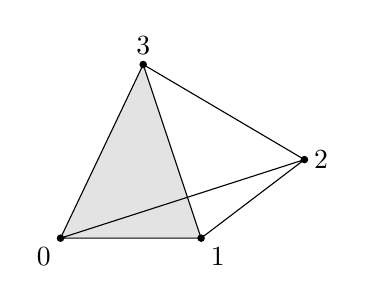
\begin{tikzpicture}[scale=1.05]
\coordinate (A) at (0,0); \coordinate (B) at (1.7,0); \coordinate (C) at (2.95,0.95); \coordinate (D) at (1.0,2.1);
\fill[gray!22] (A)--(B)--(D)--cycle;
\draw (A)--(B)--(C)--cycle;
\draw (A)--(D); \draw (B)--(D); \draw (C)--(D);
\foreach \P in {A,B,C,D} {\fill (\P) circle (1.3pt);}
\node[below left] at (A) {0}; \node[below right] at (B) {1};
\node[right] at (C) {2}; \node[above] at (D) {3};
\end{tikzpicture}
\par\smallskip{\small 图 1\quad 3-单形 $\Delta^{3}$}
\end{center}

\begin{exercise}\label{L3-4.3}
设 $\Delta^{1}\times\Delta^{1}$ 是 $\Set_{\Delta}$ 中的乘积。找出 $\Delta^{1}\times\Delta^{1}$ 中所有非退化单形。
\end{exercise}

\begin{center}
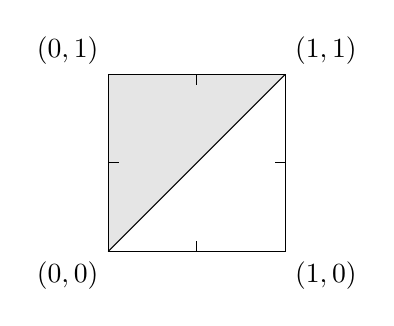
\begin{tikzpicture}[scale=1.5]
\fill[gray!20] (0,0)--(1.5,1.5)--(0,1.5)--cycle;
\draw (0,0) rectangle (1.5,1.5);
\draw (0,0)--(1.5,1.5);
\draw (0.75,0)--(0.75,0.09); \draw (0.75,1.5)--(0.75,1.41);
\draw (0,0.75)--(0.09,0.75); \draw (1.5,0.75)--(1.41,0.75);
\node[below left] at (0,0) {$(0,0)$};
\node[below right] at (1.5,0) {$(1,0)$};
\node[above right] at (1.5,1.5) {$(1,1)$};
\node[above left] at (0,1.5) {$(0,1)$};
\end{tikzpicture}
\par\smallskip{\small 图 2\quad 乘积 $\Delta^{1}\times\Delta^{1}$}
\end{center}

\begin{exercise}\label{L3-4.4}
在上例中，若在单纯集的定义中不允许退化，即把 $\Delta$ 换成 $\Delta_{\mathrm{inj}}$，会发生什么？
\end{exercise}

\begin{example}\label{L3-4.5}
令
\[
\partial\Delta^{n}\defeq\mathrm{sk}_{n-1}(\Delta^{n})
\]
为 $\Delta^{n}$ 的 $(n-1)$-骨架。我们称它为 $\Delta^{n}$ 的\textbf{边界}。
\end{example}

\begin{center}
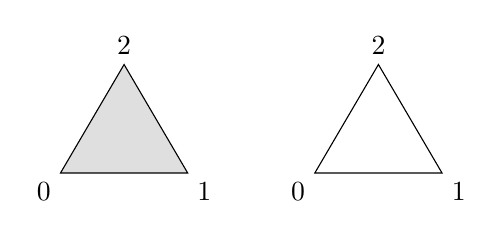
\begin{tikzpicture}[scale=0.95]
\fill[gray!25] (0,0)--(1.7,0)--(0.85,1.45)--cycle;
\draw (0,0)--(1.7,0)--(0.85,1.45)--cycle;
\node[below left] at (0,0) {0}; \node[below right] at (1.7,0) {1}; \node[above] at (0.85,1.45) {2};
\begin{scope}[xshift=3.4cm]
\draw (0,0)--(1.7,0)--(0.85,1.45)--cycle;
\node[below left] at (0,0) {0}; \node[below right] at (1.7,0) {1}; \node[above] at (0.85,1.45) {2};
\end{scope}
\end{tikzpicture}
\par\smallskip{\small 图 3\quad 2-单形 $\Delta^{2}$ 及其边界 $\partial\Delta^{2}$}
\end{center}

\begin{example}\label{L3-4.6}
令 $\Lambda^{n}_{i}$ 为 $\Delta^{n}$ 的不包含唯一非退化 $n$-单形的第 $i$ 个面的最大单纯子集。我们称它为 $\Delta^{n}$ 的第 $i$ 个\textbf{角}。
\end{example}

\begin{center}
\begin{tikzpicture}[scale=0.85]
\begin{scope}
\draw (0,0)--(1.5,0); \draw (0,0)--(0.75,1.25);
\node[below left] at (0,0) {0}; \node[below right] at (1.5,0) {1}; \node[above] at (0.75,1.25) {2};
\node[below] at (0.75,-0.75) {$\Lambda^{2}_{0}$};
\end{scope}
\begin{scope}[xshift=2.6cm]
\draw (0,0)--(1.5,0); \draw (1.5,0)--(0.75,1.25);
\node[below left] at (0,0) {0}; \node[below right] at (1.5,0) {1}; \node[above] at (0.75,1.25) {2};
\node[below] at (0.75,-0.75) {$\Lambda^{2}_{1}$};
\end{scope}
\begin{scope}[xshift=5.2cm]
\draw (0,0)--(0.75,1.25); \draw (1.5,0)--(0.75,1.25);
\node[below left] at (0,0) {0}; \node[below right] at (1.5,0) {1}; \node[above] at (0.75,1.25) {2};
\node[below] at (0.75,-0.75) {$\Lambda^{2}_{2}$};
\end{scope}
\end{tikzpicture}
\par\smallskip{\small 图 4\quad 角 $\Lambda^{2}_{0},\Lambda^{2}_{1},\Lambda^{2}_{2}$}
\end{center}

\nitem\label{L3-4.7}
读者可以用下述练习自娱，以检验对定义的理解。

\begin{exercise}\label{L3-4.8}
分类 $\Delta^{2}$ 的所有单纯商集，即在 $\Set_{\Delta}$ 中配有满射 $\Delta^{2}\to X$ 的单纯集 $X$。提示：共有 31 个。
\end{exercise}

\begin{center}
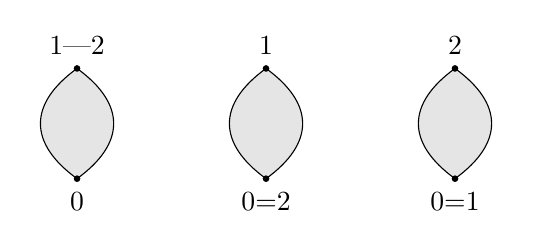
\begin{tikzpicture}[scale=1.0]
\begin{scope}
\fill[gray!20] (0,0) .. controls (-0.62,0.45) and (-0.62,0.95) .. (0,1.4) .. controls (0.62,0.95) and (0.62,0.45) .. (0,0);
\draw (0,0) .. controls (-0.62,0.45) and (-0.62,0.95) .. (0,1.4) .. controls (0.62,0.95) and (0.62,0.45) .. (0,0);
\fill (0,0) circle (1.2pt); \fill (0,1.4) circle (1.2pt);
\node[below] at (0,-0.05) {0}; \node[above] at (0,1.45) {1\text{—}2};
\end{scope}
\begin{scope}[xshift=2.4cm]
\fill[gray!20] (0,0) .. controls (-0.62,0.45) and (-0.62,0.95) .. (0,1.4) .. controls (0.62,0.95) and (0.62,0.45) .. (0,0);
\draw (0,0) .. controls (-0.62,0.45) and (-0.62,0.95) .. (0,1.4) .. controls (0.62,0.95) and (0.62,0.45) .. (0,0);
\fill (0,0) circle (1.2pt); \fill (0,1.4) circle (1.2pt);
\node[below] at (0,-0.05) {0=2}; \node[above] at (0,1.45) {1};
\end{scope}
\begin{scope}[xshift=4.8cm]
\fill[gray!20] (0,0) .. controls (-0.62,0.45) and (-0.62,0.95) .. (0,1.4) .. controls (0.62,0.95) and (0.62,0.45) .. (0,0);
\draw (0,0) .. controls (-0.62,0.45) and (-0.62,0.95) .. (0,1.4) .. controls (0.62,0.95) and (0.62,0.45) .. (0,0);
\fill (0,0) circle (1.2pt); \fill (0,1.4) circle (1.2pt);
\node[below] at (0,-0.05) {0=1}; \node[above] at (0,1.45) {2};
\end{scope}
\end{tikzpicture}
\par\smallskip{\small 图 5\quad $\Delta^{2}$ 的某些商}
\end{center}

\section{单纯集与拓扑空间}

\nitem\label{L3-5.1}
单纯范畴 $\Delta$ 可以如下实现为 $\Top$ 的子范畴。

\begin{construction}\label{L3-5.2}
令
\[
|\Delta^{n}|\defeq\{(x_{0},\dots,x_{n})\in\R^{n+1}_{\ge 0}\mid x_{0}+\cdots+x_{n}=1\}
\]
为标准（拓扑）$n$-单形。我们有函子
\begin{equation}\label{L3-eq5.1}
\Delta\to\Top,\qquad [n]\mapsto|\Delta^{n}|
\end{equation}
它把函子 $f\colon[m]\to[n]$ 送到连续映射
\[
|\Delta^{m}|\to|\Delta^{n}|,\qquad
(y_{0},\dots,y_{m})\mapsto\Bigl(\sum_{j\in f^{-1}(0)}y_{j},\dots,\sum_{j\in f^{-1}(n)}y_{j}\Bigr).
\]
\end{construction}

\begin{proposition}\label{L3-5.3}
我们通过 Yoneda 嵌入把 $\Delta$ 视为 $\Set_{\Delta}$ 的全子范畴。则函子~\eqref{L3-eq5.1} 可以延拓为保余极限的函子
\[
|-|\colon\Set_{\Delta}\to\Top,
\]
它在唯一等价的意义下唯一。我们称它为\textbf{几何实现}函子。

该函子有右伴随，由
\[
\Sing\colon\Top\to\Set_{\Delta},\qquad X\mapsto\Hom_{\Top}(|\Delta^{\bullet}|,X)
\]
给出。我们称它为\textbf{奇异单纯复形}函子\footnote{更好的名字是奇异单纯集函子，因为我们允许退化。}。
\end{proposition}

\nitem\label{L3-5.4}
伴随对
\[
|-|\colon\Set_{\Delta}\rightleftarrows\Top:\Sing
\]
属于范畴论中的下述范式。

\begin{exercise}\label{L3-5.5}
设 $\cC_{0}$ 是小范畴。定义 $\cC_{0}$ 上的\textbf{预层范畴}为
\[
\mathrm{PShv}(\cC_{0})\defeq\Fun(\cC_{0}^{\op},\Set).
\]
\begin{enumerate}[label=(\arabic*),leftmargin=2.4em,itemsep=0.1em]
\item 证明 $\mathrm{PShv}(\cC_{0})$ 是由 $\cC_{0}$ 在小余极限下自由生成的范畴。换言之，对任意含全体小余极限的范畴 $\cD$，Yoneda 嵌入 $\cC_{0}\to\mathrm{PShv}(\cC_{0})$ 诱导等价
\[
\mathrm{LFun}(\mathrm{PShv}(\cC_{0}),\cD)\simeq\Fun(\cC_{0},\cD),
\]
其中 $\mathrm{LFun}(-,-)\subset\Fun(-,-)$ 由保余极限的函子组成。
\item 设 $F\colon\mathrm{PShv}(\cC_{0})\to\cD$ 是延拓 $F_{0}\colon\cC_{0}\to\cD$ 的保余极限函子。证明 $F$ 有右伴随，由
\[
G\colon\cD\to\mathrm{PShv}(\cC_{0}),\qquad d\mapsto\Hom_{\cD}(F_{0}(-),d)
\]
给出。
\end{enumerate}
\end{exercise}

\begin{exercise}\label{L3-5.6}
挑战：对函子 $\Delta\to\Cat$ 应用上述范式，构造伴随对 $L\colon\Set_{\Delta}\rightleftarrows\Cat:R$。描述 §4 中的单纯集在该函子下的像。
\end{exercise}

\nitem\label{L3-5.7}
与脉函子 $\mathbf{N}_{\bullet}\colon\Cat\to\Set_{\Delta}$ 不同，函子 $\Sing\colon\Top\to\Set_{\Delta}$ 不是全忠实的。因此我们无法把拓扑空间的理论嵌入单纯集的理论。尽管如此，下述由 Quillen 在 1960 年代建立的结果（见 [Qui67]）说，二者的同伦论是相同的。

\begin{theorem}[Quillen]\label{L3-5.8}
伴随对
\[
|-|\colon\Set_{\Delta}\rightleftarrows\Top:\Sing
\]
诱导拓扑空间与单纯集的同伦论之间的等价。
\end{theorem}

\section{$\Set_{\Delta}$ 上的经典模型结构}

\nitem\label{L3-6.1}
为解释 Quillen 的结果，我们需要先定义 $\Set_{\Delta}$ 上的模型结构。

\begin{theoremdef}\label{L3-6.2}
$\Set_{\Delta}$ 上存在一个模型结构，由以下给出：
\begin{itemize}[leftmargin=3.4em,itemsep=0.15em]
\item [(W)] \textbf{弱同伦等价}是态射 $f\colon X\to Y$，使得
$|f|\colon|X_{\bullet}|\to|Y_{\bullet}|$ 是弱同伦等价。
\item [(C)] \textbf{上纤维化}是单态射。
\item [(F)] \textbf{Kan 纤维化}是态射 $f\colon X\to Y$，它对所有角包含 $\Lambda^{n}_{i}\to\Delta^{n}$（$0\le i\le n$、$n\ge 2$）具有右提升性质：
\begin{center}
\begin{tikzcd}[column sep=3.4em,row sep=2.6em]
\Lambda^{n}_{i}\arrow[r]\arrow[d,hook]\arrow[dr,dashed] & X\arrow[d,"f"]\\
\Delta^{n}\arrow[r] & Y.
\end{tikzcd}
\end{center}
\end{itemize}
我们称它为 $\Set_{\Delta}$ 上的\textbf{经典}模型结构，或 \textbf{Kan--Quillen 模型结构}。

该模型范畴中的纤维对象称为 \textbf{Kan 复形}。令 $\Kan\subset\Set_{\Delta}$ 为由 Kan 复形构成的全子范畴。
\end{theoremdef}

\begin{exercise}\label{L3-6.3}
找出 $\Delta^{1}$ 的一个纤维替换，即一个弱同伦等价 $\Delta^{1}\to X$，其中 $X$ 是 Kan 复形。
\end{exercise}

\begin{exercise}\label{L3-6.4}
找出 $\partial\Delta^{2}$ 的一个纤维替换。
\end{exercise}

\begin{exercise}\label{L3-6.5}
挑战：对 Kan 复形 $X$，在 $\Set_{\Delta}[W^{-1}]$ 中构造 $X$ 与 $X^{\op}$ 之间的典范同构。提示：扭曲箭头。
\end{exercise}

\begin{remark}\label{L3-6.6}
可以不用几何实现函子来定义单纯集之间的弱同伦等价。我们这样定义：
\begin{itemize}[leftmargin=3.4em,itemsep=0.15em]
\item [(W)] \textbf{弱同伦等价}是态射 $f\colon X\to Y$，使得对任意 Kan 复形 $Z$，映射
\[
[Y,Z]\to[X,Z]
\]
是双射，其中集合 $[X,Z]$ 是
\[
\Hom_{\Set_{\Delta}}(X\times\Delta^{1},Z)\rightrightarrows\Hom_{\Set_{\Delta}}(X,Z)
\]
的余等化子。
\end{itemize}
由 Quillen 定理~\ref{L3-5.8}（其精确形式见定理~\ref{L3-8.1}）与 Yoneda 引理，这两个定义事后是等价的。然而，选这一个定义还是那一个，会显著影响检验模型范畴公理与证明 Quillen 定理的方式。对本课程而言，这些证明被当作黑箱，读者不妨把两种陈述都当作定义。
\end{remark}

\section{同伦论之间的等价}

\nitem\label{L3-7.1}
本节解释两个同伦论之间等价的意义。设 $F\colon\cC\rightleftarrows\cD:G$ 是模型范畴之间的伴随对\footnote{我们不要求 $F$ 或 $G$ 保持 (W) 或 (C) 或 (F)。}。我们需要回答下述问题：
\begin{center}
\emph{这个伴随对何时诱导 $\cC$ 与 $\cD$ 底层的同伦论之间的等价？}
\end{center}
答案将是
\begin{itemize}[leftmargin=2.2em,itemsep=0.1em]
\item 伴随对 $F\colon\cC\rightleftarrows\cD:G$ 应诱导伴随对
\[
F^{\prime}\colon\cC[W^{-1}]\rightleftarrows\cD[W^{-1}]:G^{\prime},
\]
使得 $F^{\prime}$ 与 $G^{\prime}$ 互为逆\footnote{经典术语是拟逆（quasi-inverse），即要求 $\id\to G^{\prime}\circ F^{\prime}$ 与 $F^{\prime}\circ G^{\prime}\to\id$ 是等价而非相等。后一要求违背等价原则，因而在高阶范畴论中没有意义。因此我们省去前缀“拟”。}。
\end{itemize}
然而，要让它有意义，我们需要说清函子 $F^{\prime}$ 与 $G^{\prime}$ 的定义。这样一个定义的试金石是下述来自同调代数的例子。

\begin{example}\label{L3-7.2}
设 $A_{i}$ 是 Abel 范畴，使得 $\Ch^{\le 0}(A_{i})$ 上的投射模型结构有良好定义（见第 2 讲例 2.7）。我们有
\[
\Ch^{\le 0}(A_{i})[W^{-1}]\simeq\mathrm{D}^{\le 0}(A_{i}),
\]
其中 $\mathrm{D}^{\le 0}(A_{i})$ 是 $A_{i}$ 的导出范畴的连通（＝非正）部分。设 $F_{0}\colon A_{1}\to A_{2}$ 是加性函子，并考虑由 $F_{0}$ 诱导的函子
\[
F\colon\Ch^{\le 0}(A_{1})\to\Ch^{\le 0}(A_{2}).
\]
则我们希望 $F^{\prime}$ 是\textbf{左导出函子} $\mathbb{L}F$，它可由
\[
\mathbb{L}F(M^{\bullet})\simeq F(P^{\bullet})
\]
计算，其中 $P^{\bullet}\to M^{\bullet}$ 是 $M^{\bullet}$ 的上纤维替换，亦即投射消解。

需要对函子 $F_{0}$ 作额外假设，才能保证 $F(P^{\bullet})\in\mathrm{D}^{\le 0}(A_{2})$ 不依赖 $P^{\bullet}$ 的选取。
\end{example}

\begin{example}\label{L3-7.3}
对偶地，对单射模型范畴 $\Ch^{\ge 0}(A_{i})$，我们希望恢复\textbf{右导出函子}的定义。
\end{example}

\nitem\label{L3-7.4}
注意在上例中，函子 $F$ 不保持拟同构（因为 $F_{0}$ 不正合）。因此在 §7.1 的一般框架下，我们不应当要求 $F$ 或 $G$ 保持\emph{所有}对象之间的弱等价。特别地，我们不能指望下述图交换：
\begin{center}
\begin{tikzcd}[column sep=4.6em,row sep=2.4em]
\cC\arrow[r]\arrow[d,"F"'] & \cC[W^{-1}]\arrow[d,"F^{\prime}"]\\
\cD\arrow[r] & \cD[W^{-1}]
\end{tikzcd}
\end{center}
不过，在同调代数中，导出函子给出了这种交换方形的最佳逼近。为解释其含义，我们需要一些定义。

\begin{definition}\label{L3-7.5}
设 $\pi\colon\cC\to\cC^{\prime}$ 是范畴之间的函子。对任意范畴 $\cE$，我们有函子
\[
\pi^{*}\colon\Fun(\cC^{\prime},\cE)\to\Fun(\cC,\cE),
\]
由沿 $\pi$ 前复合给出。该函子的左（相应地，右）伴随（当存在时）称为沿 $\pi$ 的\textbf{左（相应地，右）Kan 扩张}，并记作
\[
\mathrm{LKE}_{\pi}\colon\Fun(\cC,\cE)\to\Fun(\cC^{\prime},\cE),\qquad
\mathrm{RKE}_{\pi}\colon\Fun(\cC,\cE)\to\Fun(\cC^{\prime},\cE).
\]
\end{definition}

\begin{exercise}\label{L3-7.6}
设 $f\colon\cC\to\cE$ 是函子，找出刻画函子 $\mathrm{LKE}_{\pi}f$ 与 $\mathrm{RKE}_{\pi}f$ 的泛性质。提示：
\begin{center}
\begin{tikzcd}[column sep=2.4em,row sep=1.7em]
& \cC^{\prime}\arrow[dr,dotted,"{\mathrm{LKE}_{\pi}f}"'] & \\
\cC\arrow[ur,"\pi"']\arrow[rr,"f"'] & ?\arrow[u,dotted] & \cD
\end{tikzcd}
\qquad
\begin{tikzcd}[column sep=2.4em,row sep=1.7em]
& \cC^{\prime}\arrow[dr,dotted,"{\mathrm{RKE}_{\pi}f}"']\arrow[d,dotted] & \\
\cC\arrow[ur,"\pi"']\arrow[rr,"f"'] & ? & \cD
\end{tikzcd}
\end{center}
最接近交换。
\end{exercise}

\begin{example}\label{L3-7.7}
设 $F_{0}\colon A_{1}\to A_{2}$ 同例~\ref{L3-7.2}。则左导出函子
\[
\mathbb{L}F\colon\mathrm{D}^{\le 0}(A_{1})\to\mathrm{D}^{\le 0}(A_{2})
\]
定义为函子
\[
\Ch^{\le 0}(A_{1})\xrightarrow{F}\Ch^{\le 0}(A_{2})\xrightarrow{\pi_{2}}\mathrm{D}^{\le 0}(A_{2})
\]
沿
\[
\Ch^{\le 0}(A_{1})\xrightarrow{\pi_{1}}\mathrm{D}^{\le 0}(A_{1})
\]
的右 Kan 扩张\footnote{这种手性的反转虽令人不快，却无法避免。}。用图表示：
\begin{equation}\label{L3-eq7.1}
\begin{tikzcd}[column sep=5.2em,row sep=2.8em]
\Ch^{\le 0}(A_{1})\arrow[r,"\pi_{1}"]\arrow[d,"F"'] & \mathrm{D}^{\le 0}(A_{1})\arrow[d,"{\mathbb{L}F\defeq\mathbb{R}\mathrm{KE}_{\pi_{1}}(\pi_{2}\circ F)}"]\\
\Ch^{\le 0}(A_{2})\arrow[r,"\pi_{2}"']\arrow[ur,dotted] & \mathrm{D}^{\le 0}(A_{2}).
\end{tikzcd}
\end{equation}
类似地，右导出函子定义为左 Kan 扩张。
\end{example}

\begin{exercise}\label{L3-7.8}
通过把~\eqref{L3-eq7.1} 作用在复形 $M^{\bullet}$ 上，说服自己左导出函子应当是右 Kan 扩张而不是左 Kan 扩张。
\end{exercise}

\nitem\label{L3-7.9}
受上述内容启发，我们可以在同伦代数中定义导出函子。

\begin{definition}\label{L3-7.10}
设 $F\colon\cC\to\cD$ 是模型范畴之间的（普通）函子。$F$ 的\textbf{左导出函子}
\[
\mathbb{L}F\colon\cC[W^{-1}]\to\cD[W^{-1}]
\]
定义为下述右 Kan 扩张
\begin{equation}\label{L3-eq7.2}
\begin{tikzcd}[column sep=4.6em,row sep=2.8em]
\cC\arrow[r]\arrow[d,"F"'] & \cC[W^{-1}]\arrow[d,"{\mathbb{L}F\defeq\mathbb{R}\mathrm{KE}}"]\\
\cD\arrow[r]\arrow[ur,dotted] & \cD[W^{-1}].
\end{tikzcd}
\end{equation}
类似地，右导出函子定义为左 Kan 扩张。
\end{definition}

\begin{remark}\label{L3-7.11}
我们可以滥用记号，把自然变换~\eqref{L3-eq7.2} 写成 $\cD[W^{-1}]$ 中的态射
\[
\mathbb{L}F(X)\to F(X),
\]
这些态射对 $X$ 在 $\cC$ 中函子化。

类似地，对函子 $G\colon\cD\to\cC$，我们有 $\cC[W^{-1}]$ 中的态射
\[
G(Y)\to\mathbb{R}G(Y),
\]
它们对 $Y$ 在 $\cD$ 中函子化。
\end{remark}

\nitem\label{L3-7.12}
注意导出函子的定义没有用到上纤维化与纤维化这两类态射。下述结果提供了用这些态射计算导出函子的便利工具。参见 [DS95, §9]。

\begin{theorem}\label{L3-7.13}
设 $F\colon\cC\to\cD$ 与 $G\colon\cD\to\cC$ 是模型范畴之间的函子。
\begin{enumerate}[label=(\arabic*),leftmargin=2.4em,itemsep=0.1em]
\item 假设 $F$ 把上纤维对象之间的弱等价送到弱等价。则左导出函子 $\mathbb{L}F$ 存在。此外，对 $\cC$ 中任意上纤维对象 $X$，有 $\mathbb{L}F(X)\xrightarrow{\ \simeq\ }F(X)$。
\item 假设 $G$ 把纤维对象之间的弱等价送到弱等价。则右导出函子 $\mathbb{R}G$ 存在。此外，对 $\cD$ 中任意纤维对象 $Y$，有 $G(Y)\xrightarrow{\ \simeq\ }\mathbb{R}G(Y)$。
\end{enumerate}
\end{theorem}

\begin{exercise}\label{L3-7.14}
解释如何用上纤维/纤维替换计算左/右导出函子。对例~\ref{L3-7.2} 你会得到什么？
\end{exercise}

\nitem\label{L3-7.15}
受上述内容启发，我们作下述定义。

\begin{proposition}\label{L3-7.16}
设 $F\colon\cC\rightleftarrows\cD:G$ 是模型范畴之间的伴随对。下述条件等价：
\begin{enumerate}[label=(\roman*),leftmargin=2.4em,itemsep=0.1em]
\item $F$ 保持上纤维化与无环上纤维化；
\item $G$ 保持纤维化与无环纤维化；
\item $F$ 保持上纤维化，且 $G$ 保持纤维化；
\item $F$ 保持无环上纤维化，且 $G$ 保持无环纤维化。
\end{enumerate}
当这些条件成立时，我们说 $F\colon\cC\rightleftarrows\cD:G$ 是 \textbf{Quillen 伴随}，并称 $F$（相应地，$G$）为左（相应地，右）\textbf{Quillen 函子}。
\end{proposition}

\begin{exercise}\label{L3-7.17}
设 $F\colon\cC\rightleftarrows\cD:G$ 是 Quillen 伴随。证明定理~\ref{L3-7.13} 中的条件成立。
\end{exercise}

\begin{proposition}\label{L3-7.18}
设 $F\colon\cC\rightleftarrows\cD:G$ 是 Quillen 伴随。我们有自然的伴随
\[
\mathbb{L}F\colon\cC[W^{-1}]\rightleftarrows\cD[W^{-1}]:\mathbb{R}G.
\]
\end{proposition}

\nitem\label{L3-7.19}
我们终于可以给同伦论之间的等价一个精确定义。

\begin{definition}\label{L3-7.20}
Quillen 伴随 $F\colon\cC\rightleftarrows\cD:G$ 称为 \textbf{Quillen 等价}，若诱导的伴随
\[
\mathbb{L}F\colon\cC[W^{-1}]\rightleftarrows\cD[W^{-1}]:\mathbb{R}G
\]
是范畴之间的等价。
\end{definition}

\section{结论}

\begin{theorem}[Quillen]\label{L3-8.1}
伴随对
\[
|-|\colon\Set_{\Delta}\rightleftarrows\Top:\Sing
\]
是两侧经典模型结构之间的 Quillen 等价。
\end{theorem}

\nitem\label{L3-8.2}
上述定理连同同伦假设，为下述定义提供了依据。

\begin{definition}\label{L3-8.3}
记
\[
\hGrpd_{\infty}\defeq\Set_{\Delta}[W^{-1}],\qquad h\Spc\defeq\Set_{\Delta}[W^{-1}],
\]
并分别称它们为 $\infty$-群胚的同伦范畴与空间的同伦范畴\footnote{我们引入新记号 $h\Spc$ 而不用 $\hTop$，是因为在后续几讲中我们将构造空间的 $\infty$-范畴 $\Spc$，它需要与拓扑空间的普通范畴 $\Top$ 相区分。}。
\end{definition}

\yizhu{定义中 $\hGrpd_{\infty}$ 与 $h\Spc$ 取同一个局部化范畴，这正是同伦假设的断言：$\infty$-群胚的同伦论就是空间的同伦论；两个名字只是强调同一对象的两面。\textbf{[来源：I]}}

\begin{remark}\label{L3-8.4}
在上述定义中，我们用 $\Set_{\Delta}[W^{-1}]$ 而不用 $h\Set_{\Delta}$，理由有二。

第一条理由是实用的。我们不想为每个 $\infty$-群胚指定一个具体的 Kan 复形。这会带来不便，因为许多关于 Kan 复形的构造只在典范弱等价的意义下良好定义\footnote{比较：我们也不想为 $\mathrm{D}^{\le 0}(A)$ 中每个对象指定一个具体的投射对象复形。}。

第二条理由是审美上的。局部化范畴 $\Set_{\Delta}[W^{-1}]$ 能以模型无关的方式升级为 $\infty$-范畴，因为定义它的泛性质对 $\infty$-范畴有意义。这给出了小 $\infty$-群胚的 $\infty$-范畴 $\Grpd_{\infty}$ 的一个构造。另一方面，任何已知的 $h\Set_{\Delta}$ 到 $\infty$-范畴的升级都依赖于 $\infty$-范畴模型的选择。
\end{remark}

\nitem\label{L3-8.5}
在后续几讲中，我们将构造 Quillen 等价
\[
\mathfrak{C}\colon\Set^{Joyal}_{\Delta}\rightleftarrows\Cat_{\Delta}:\mathfrak{N},
\]
其中
\begin{itemize}[leftmargin=2.2em,itemsep=0.1em]
\item $\Set^{Joyal}_{\Delta}$ 是单纯集范畴上的 \textbf{Joyal 模型结构}；
\item $\Cat_{\Delta}$ 是小\textbf{单纯范畴}的范畴，即以 $\Set_{\Delta}$ 充实的范畴。我们将给它配备由 $\Set_{\Delta}$ 上\textbf{经典}模型结构诱导的模型结构。
\end{itemize}
这将识别这些模型范畴底层的同伦论。另一方面，Quillen 定理~\ref{L3-8.1} 蕴含 $\Cat_{\Delta}$ 与 $\Cat_{\Top}$ 的同伦论等价。结合同伦假设（[第 2 讲口号 0.1]），我们将得到下述命题的有力证据：
\begin{center}
\emph{$(\infty,1)$-范畴的理论 $=$ $\Set^{Joyal}_{\Delta}$ 底层的同伦论。}
\end{center}

\appendixsection{再论 Quillen 伴随}

\begin{exercise}\label{L3-A.1}
设 $\cC$ 与 $\cD$ 是模型范畴。假设有伴随对 $F^{\prime}\colon\cC[W^{-1}]\rightleftarrows\cD[W^{-1}]:G^{\prime}$，是否总能把它提升为 Quillen 伴随？Quillen 等价又如何？
\end{exercise}

\nitem\label{L3-A.2}
\textbf{建议阅读}：\quad [DS09]。

\appendixsection{Quillen 的余切复形}

\begin{exercise}\label{L3-B.1}
人们说：
\begin{center}
\emph{余切复形函子是 Kähler 微分函子的左导出函子。}
\end{center}
请用模型范畴的导出函子让这句话有意义。
\end{exercise}

\nitem\label{L3-B.2}
\textbf{建议阅读}。[And67]、[And74]、[Qui70]（原始文献）与 [Iye07]（较近的文献）。

\subsection*{参考文献}
\par\noindent\hangindent=5.2em\hangafter=1 [And67]\hspace{0.6em}Michel Andr\'e. \emph{M\'ethode simpliciale en alg\`ebre homologique et alg\`ebre commutative}, volume 32. Springer, 1967.
\par\noindent\hangindent=5.2em\hangafter=1 [And74]\hspace{0.6em}Michel Andr\'e. \emph{Homologie des algebres commutatives}, volume 206. Springer, 1974.
\par\noindent\hangindent=5.2em\hangafter=1 [DS95]\hspace{0.6em}William G Dwyer and Jan Spalinski. Homotopy theories and model categories. \emph{Handbook of algebraic topology}, 73(126):21, 1995.
\par\noindent\hangindent=5.2em\hangafter=1 [DS09]\hspace{0.6em}Daniel Dugger and Brooke Shipley. A curious example of triangulated-equivalent model categories which are not Quillen equivalent. \emph{Algebraic \& Geometric Topology}, 9(1):135--166, 2009.
\par\noindent\hangindent=5.2em\hangafter=1 [Iye07]\hspace{0.6em}Srikanth Iyengar. Andr\'e--Quillen homology of commutative algebras. \emph{Contemporary Mathematics}, 436:203, 2007.
\par\noindent\hangindent=5.2em\hangafter=1 [Qui67]\hspace{0.6em}Daniel G Quillen. \emph{Homotopical algebra}. Lecture Notes in Mathematics, 1967.
\par\noindent\hangindent=5.2em\hangafter=1 [Qui70]\hspace{0.6em}Daniel Quillen. On the (co-) homology of commutative rings. In \emph{Proc. Symp. Pure Math}, volume 17, pages 65--87, 1970.
}{}
\IfFileExists{chunks/lec04.tex}{% =============================================================================
%  lec04.tex —— 第 4 讲 拟范畴（底本 PDF 第 28–38 页）
% =============================================================================
\lecture{4}{拟范畴}
\begin{center}\small\color{black!55}（底本 PDF 第 28–38 页）\end{center}

就本课程的目的而言，本讲不给出证明，也不按逻辑顺序陈述结论。

\section{拟范畴}

\nitem\label{L4-1.1} 上次课我们构造了 Quillen 等价
\[
|{-}|\colon \Set_\Delta \rightleftarrows \Top \colon \Sing.
\]
由此可得：
\begin{itemize}[leftmargin=2.2em,itemsep=0.1em]
\item 任何 $\infty$-群胚——由同伦假设，它可以等同于一个同伦型——也可以实现为 $\Set_\Delta$ 中的双纤维对象，即 Kan 复形。
\item $\infty$-群胚之间的任何函子都可以实现为相应 Kan 复形之间态射的同伦类。这里，两个态射 $f,g\colon X\to Y$ 同伦，当且仅当存在态射 $H\colon X\times\Delta^1\to Y$，使得 $H(-,0)=f$ 且 $H(-,1)=g$。
\end{itemize}

\nitem\label{L4-1.2} 回顾：单纯集 $X$ 是 Kan 复形，当且仅当它对所有 $n\ge 2$ 的角嵌入
\[
\begin{tikzcd}[column sep=3.4em,row sep=2.6em]
\Lambda^n_i \arrow[r] \arrow[d] & X \\
\Delta^n \arrow[ur, dashed] &
\end{tikzcd}
\]
具有右提升性质。下面我们用高阶范畴论的语言，考察不同 $(n,i)$ 选择下的这些提升性质。

\nitem\label{L4-1.3} 当 $n=2$、$i=0$ 时，提升性质说的是：给定态射 $f\colon x_0\to x_1$，任何形如 $x_0\to x_2$ 的态射都可以通过 $f$ 分解。当 $n=3$、$i=0$ 时，提升性质说的是：给定态射 $f\colon x_0\to x_1$，任何交换图
\[
\begin{tikzcd}[column sep=3.2em,row sep=2.2em]
& x_2 \arrow[dr] & \\
x_0 \arrow[ur] \arrow[rr] & & x_3
\end{tikzcd}
\]
——或者更确切地说，见证这样一个图的可逆 $2$-态射——都可以通过 $f$ 分解。这意味着上述 $2$-态射等价于一个 $2$-态射
\[
\begin{tikzcd}[column sep=3.2em,row sep=2.2em]
& x_2 \arrow[dr] & \\
x_1 \arrow[ur] \arrow[rr] & & x_3
\end{tikzcd}
\]
与恒等 $2$-态射 $\id_f$ 的横复合。

\nitem\label{L4-1.4} 对偶地，$i=n$ 时的提升性质说的是：给定态射 $f\colon x\to y$，任何以 $y$ 为末顶点的同伦连贯图都可以通过 $f$ 分解。同样，这是 $\infty$-群胚而非一般 $\infty$-范畴的特征：它蕴含给定的态射 $f$ 有右逆。

\nitem\label{L4-1.5} 另一方面，$0<i<n$ 时的提升性质说的是：给定对象 $x$，可以把任何以 $x$ 为末顶点的同伦连贯图与另一个以 $x$ 为首顶点的同伦连贯图复合起来。任何像范畴的数学实体都应当满足这一要求。

\nitem\label{L4-1.6} 上述讨论促使我们作如下定义：

\begin{definition}\label{L4-1.7}
（Boardman--Vogt，1973）单纯集 $X$ 称为\textbf{拟范畴}（quasi-category），若它对内角嵌入
\[
\begin{tikzcd}[column sep=3.4em,row sep=2.6em]
\Lambda^n_i \arrow[r] \arrow[d] & X \\
\Delta^n \arrow[ur, dashed] &
\end{tikzcd}
\qquad (0<i<n)
\]
具有右提升性质。
\end{definition}

\yizhu{拟范畴又称弱 Kan 复形：这一概念由 Boardman 与 Vogt 在 1973 年引入，1980 年代由 Joyal 系统发展，并命名为拟范畴（quasi-category）；Joyal 于 2002 年证明了拟范畴正是 $(\infty,1)$-范畴的一类模型。\textbf{[来源：A：Boardman--Vogt, \emph{Homotopy Invariant Algebraic Structures on Topological Spaces}, 1973；Joyal, \emph{Quasi-categories and Kan complexes}, 2002]}}

设 $X$ 是拟范畴。我们把 $0$-单形 $x\in X_0$ 称为 $X$ 的\textbf{对象}，把 $1$-单形 $e\in X_1$ 称为从 $d^1_0(e)$ 到 $d^1_1(e)$ 的\textbf{态射}。

设 $X$ 与 $Y$ 是拟范畴，我们把 $\Set_\Delta$ 中的态射 $F\colon X\to Y$ 称为从 $X$ 到 $Y$ 的\textbf{函子}。

设 $\mathrm{QCat}\subset\Set_\Delta$ 为拟范畴构成的全子范畴。

\begin{example}\label{L4-1.8}
Kan 复形是拟范畴。
\end{example}

\begin{exercise}\label{L4-1.9}
范畴的脉是拟范畴。
\end{exercise}

\begin{exercise}\label{L4-1.10}
拟范畴的反范畴 $X^{\op}$ 是拟范畴。（见第 3 讲构造 1.14。）
\end{exercise}

\nitem\label{L4-1.11} 1980 年代，Joyal 提出：
\begin{center}
\emph{拟范畴是 $(\infty,1)$-范畴的模型。}
\end{center}
本讲把上述提法当作既定事实，并用它来发展关于 $(\infty,1)$-范畴的基本语言。我们将在下一讲为这一提法提供依据。

\section{态射的复合}

\begin{definition}\label{L4-2.1}
设 $\cC$ 是拟范畴。对形如
\[
\begin{tikzcd}[column sep=3.4em,row sep=2.4em]
& y \arrow[dr, "g"] & \\
x \arrow[ur, "f"] \arrow[rr, "h"'] & & z
\end{tikzcd}
\]
的 $2$-单形 $\sigma$，我们说 $\sigma$ \textbf{见证} $h$ 是 $f$ 与 $g$ 的复合。
\end{definition}

\begin{remark}\label{L4-2.2}
注意在上述定义中，态射 $h$ 不由 $f$ 与 $g$ 决定，$\sigma$ 也不由 $f$、$g$ 与 $h$ 决定。我们可以说：
\begin{center}
拟范畴中态射的复合不是具体的。
\end{center}
尽管如此，我们很快就会看到：只要正确理解“良定义”，由 $\cC$ 表示的 $\infty$-范畴中态射的复合就是良定义的。
\end{remark}

\section{态射之间的同伦}

\begin{definition}\label{L4-3.1}
设 $\cC$ 是拟范畴。对形如
\[
\begin{tikzcd}[column sep=3.4em,row sep=2.4em]
& y \arrow[dr, "\id"] & \\
x \arrow[ur, "f"] \arrow[rr, "g"'] & & y
\end{tikzcd}
\]
的 $2$-单形 $\sigma$，我们说 $\sigma$ 是从 $f$ 到 $g$ 的\textbf{左掐同伦}\footnote{此术语非标准。例如 [Rez22] 称之为右同伦。}，或\textbf{左掐 $2$-态射}。

对偶地，形如
\[
\begin{tikzcd}[column sep=3.4em,row sep=2.4em]
& x \arrow[dr, "f"] & \\
x \arrow[ur, "\id"] \arrow[rr, "g"'] & & y
\end{tikzcd}
\]
的 $2$-单形称为从 $f$ 到 $g$ 的\textbf{右掐同伦}，或\textbf{右掐 $2$-态射}。
\end{definition}

\yizhu{“掐”（pinched）取单形一端被捏合之意：左掐（右掐）$2$-单形的两条边中有一条是恒等态射，于是单形的两个顶点被掐合在一起。作者已注明此术语非标准，Rezk 称左掐同伦为右同伦，故阅读文献时须注意对应关系。\textbf{[译者按（无外部依据）]}}

\begin{exercise}\label{L4-3.2}
下列条件等价：
\begin{itemize}[leftmargin=2.2em,itemsep=0.1em]
\item 存在从 $f$ 到 $g$ 的左掐同伦；
\item 存在从 $f$ 到 $g$ 的右掐同伦。
\end{itemize}
此外，这些条件在从 $x$ 到 $y$ 的态射集合上定义了一个等价关系。提示：角嵌入 $\Lambda^3_1\to\Delta^3$ 与 $\Lambda^3_2\to\Delta^3$。
\end{exercise}

\begin{definition}\label{L4-3.3}
设 $\cC$ 是拟范畴，$f,g\colon x\to y$ 是态射。若它们满足上述练习中的条件，则称 $f$ \textbf{同伦于} $g$。
\end{definition}

\section{同伦范畴}

\begin{exercise}\label{L4-4.1}
设 $\cC$ 是拟范畴。证明下列构造定义了一个范畴 $h\cC$：
\begin{itemize}[leftmargin=2.2em,itemsep=0.1em]
\item $h\cC$ 的对象是 $\cC$ 的对象；
\item $h\cC$ 的态射是 $\cC$ 中态射的同伦类；
\item 在 $h\cC$ 中 $[f]$ 与 $[g]$ 的复合等于 $[h]$，当且仅当 $h$ 是 $\cC$ 中 $f$ 与 $g$ 的复合。
\end{itemize}
\end{exercise}

\begin{definition}\label{L4-4.2}
设 $\cC$ 是拟范畴。我们把上述练习中的范畴称为 $\cC$ 的\textbf{同伦范畴}，记作 $h\cC$。
\end{definition}

\begin{exercise}\label{L4-4.3}
我们有伴随对
\[
h\colon \mathrm{QCat} \rightleftarrows \Cat \colon N_{\bullet}.
\]
\end{exercise}

\begin{remark}\label{L4-4.4}
上述练习说明，$h\cC$ 是把由 $\cC$ 表示的 $\infty$-范畴中所有高阶态射强制为恒等态射后得到的范畴。注意这与放弃所有高阶态射并不相同。后一种构造是\textbf{邪恶的}，因为它违反同构原则。
\end{remark}

\nitem\label{L4-4.5} 顾名思义，拟范畴的同伦范畴与模型范畴的同伦范畴有关。我们将在以后的讲次中解释这种联系。

\section{同构}

\begin{definition}\label{L4-5.1}
设 $\cC$ 是拟范畴。若 $h\cC$ 中的态射 $[f]$ 是同构，则称态射 $f$ 是\textbf{同构}。
\end{definition}

\nitem\label{L4-5.2} 换言之，$f\colon x\to y$ 是同构，当且仅当存在态射 $g\colon y\to x$，使得 $g\circ f$ 同伦于 $\id_x$ 且 $f\circ g$ 同伦于 $\id_y$。

\begin{exercise}\label{L4-5.3}
拟范畴是 Kan 复形，当且仅当它的所有态射都是同构。
\end{exercise}

\begin{exercise}\label{L4-5.4}
对拟范畴 $\cC$，存在唯一的 Kan 复形 $\cC^{\simeq}\subset\cC$，称为 $\cC$ 的\textbf{核心}，它包含 $\cC$ 的全部同构。所得函子 $(-)^{\simeq}\colon\mathrm{QCat}\to\Kan$ 是嵌入函子 $\Kan\to\mathrm{QCat}$ 的右伴随。
\end{exercise}

\section{态射空间：想法}

\nitem\label{L4-6.1} 作为对 Joyal 提法的一次合理性检验，对拟范畴 $\cC$ 中的一对对象 $x,y$，我们应当构造一个 $\infty$-群胚 $\mathrm{Maps}_{\cC}(x,y)$，使得：
\begin{itemize}[leftmargin=2.2em,itemsep=0.1em]
\item $\mathrm{Maps}_{\cC}(x,y)$ 中的对象是从 $x$ 到 $y$ 的态射；
\item $\mathrm{Maps}_{\cC}(x,y)$ 中的态射是从 $x$ 到 $y$ 的态射之间的 $2$-态射；
\item $\cdots$
\end{itemize}
本讲给出三个代表这个 $\infty$-群胚的 Kan 复形构造（“代表”的含义见第 3 讲定义 8.3）。这三个 Kan 复形彼此弱同伦等价，但互不同构。

\nitem\label{L4-6.2} 在一个模型无关的、或公理化的 $(\infty,1)$-范畴理论\footnote{我并不知道这样的理论是否存在，因此下面的讨论仅起启发作用。}中，这三个构造应分别对应下述 $\infty$-群胚：
\begin{itemize}[leftmargin=2.6em,itemsep=0.15em,label={}]
\item[(B)] 纤维积
\[
\{x\}\times_{\Fun(\{0\},\cC)}\Fun([1],\cC)\times_{\Fun(\{1\},\cC)}\{y\},
\]
其中 $\Fun(\cD,\cC)$ 是从 $\cD$ 到 $\cC$ 的 $(\infty,1)$-范畴。
\item[(L)] 纤维积
\[
\cC_{x/}\times_{\cC}\{y\},
\]
其中 $\cC_{x/}$ 是 $\cC$ 在 $x$ 下的余切片 $(\infty,1)$-范畴。
\item[(R)] 纤维积
\[
\{x\}\times_{\cC}\cC_{/y},
\]
其中 $\cC_{/y}$ 是 $\cC$ 在 $y$ 上的切片 $(\infty,1)$-范畴。
\end{itemize}

\begin{exercise}\label{L4-6.3}
请说服自己：上述三个 $\infty$-群胚应当典范等价。
\end{exercise}

\section{函子拟范畴}

\nitem\label{L4-7.1} 为了用拟范畴实现 (B)，我们需要定义两个拟范畴之间的函子拟范畴。

\begin{definition}\label{L4-7.2}
称范畴 $\cC$ 是\textbf{笛卡尔闭}的，若它满足下列条件：
\begin{enumerate}[label=(\arabic*),leftmargin=2.4em,itemsep=0.1em]
\item $\cC$ 中有限积存在；
\item 对 $\cC$ 中任意对象 $X$ 与 $Y$，函子
\[
\Hom(X\times -,Y)\colon \cC^{\op}\to\Set
\]
余可表示，即存在对象 $Y^{X}$，称为\textbf{指数对象}，满足如下泛性质：
\[
\Hom(X\times Z,Y)\simeq\Hom(Z,Y^{X}).
\]
\end{enumerate}
\end{definition}

\begin{remark}\label{L4-7.3}
条件 (2) 等价于

(2$'$) 对任意对象 $X$，函子 $X\times -\colon \cC\to\cC$ 有右伴随。

事实上，这个右伴随由 $(-)^{X}\colon\cC\to\cC$ 给出。
\end{remark}

\begin{theoremdef}\label{L4-7.4}
范畴 $\Set_\Delta$ 是笛卡尔闭的。对单纯集 $X$ 与 $Y$，我们把指数对象记作
\[
\Fun(X,Y)\defeq Y^{X}\in\Set_\Delta.
\]
\end{theoremdef}

\begin{exercise}\label{L4-7.5}
$\Fun(X^{\op},Y^{\op})\simeq\Fun(X,Y)^{\op}$。
\end{exercise}

\begin{exercise}\label{L4-7.6}
证明脉函子 $N_{\bullet}\colon\Cat\to\Set_\Delta$ 与积和指数相容，即
\[
N_{\bullet}(\cC\times\cD)\xrightarrow{\ \simeq\ }N_{\bullet}(\cC)\times N_{\bullet}(\cD),
\qquad
N_{\bullet}(\Fun(\cC,\cD))\xrightarrow{\ \simeq\ }\Fun(N_{\bullet}(\cC),N_{\bullet}(\cD)).
\]
\end{exercise}

\begin{proposition}\label{L4-7.7}
（Ker.00TN）对 $X\in\Set_\Delta$ 与 $Y\in\Kan$，有 $\Fun(X,Y)\in\Kan$。
\end{proposition}

\begin{proposition}\label{L4-7.8}
（Ker.0066）对 $X\in\Set_\Delta$ 与 $Y\in\mathrm{QCat}$，有 $\Fun(X,Y)\in\mathrm{QCat}$。
\end{proposition}

\begin{corollary}\label{L4-7.9}
范畴 $\mathrm{QCat}$ 是笛卡尔闭的。
\end{corollary}

\begin{theoremdef}\label{L4-7.10}
（Ker.01JC）设 $\cC$ 是拟范畴，$x,y$ 是 $\cC$ 中的对象。则单纯集
\[
\Hom^{B}_{\cC}(x,y)\defeq\{x\}\times_{\Fun(\{0\},\cC)}\Fun(\Delta^1,\cC)\times_{\Fun(\{1\},\cC)}\{y\}
\]
是 Kan 复形，称为从 $x$ 到 $y$ 的\textbf{平衡态射复形}\footnote{此术语非标准。例如 Lurie 称之为态射空间。}。
\end{theoremdef}

\nitem\label{L4-7.11} 按定义，对检验单纯集 $K$，下述两个集合之间存在双射：
\begin{itemize}[leftmargin=2.2em,itemsep=0.1em]
\item 态射 $K\to\Hom^{B}_{\cC}(x,y)$；
\item 在 $K\times\{0\}$ 上取常值 $x$、在 $K\times\{1\}$ 上取常值 $y$ 的态射 $K\times\Delta^1\to\cC$。
\end{itemize}

\nitem\label{L4-7.12} 特别地，$\Hom^{B}_{\cC}(x,y)$ 中的一个 $1$-单形对应一个形如
\[
\begin{tikzcd}[column sep=3.2em,row sep=2.6em]
x \arrow[r, "f"] \arrow[d, "\id"'] \arrow[dr, dashed] & y \arrow[d, "\id"] \\
x \arrow[r, "g"'] & y
\end{tikzcd}
\]
的图 $\Delta^1\times\Delta^1\to\cC$。我们把这样的图称为从 $f$ 到 $g$ 的\textbf{平衡同伦}\footnote{此术语非标准。}，或\textbf{平衡 $2$-态射}。

\begin{exercise}\label{L4-7.13}
设 $\cC$ 是拟范畴，$f,g\colon x\to y$ 是态射。证明：$f$ 同伦于 $g$，当且仅当存在从 $f$ 到 $g$ 的平衡同伦。
\end{exercise}

\begin{exercise}\label{L4-7.14}
构造典范同构
\[
\Hom^{B}_{\cC}(x,y)^{\op}\xrightarrow{\ \simeq\ }\Hom^{B}_{\cC^{\op}}(y,x).
\]
\end{exercise}

\section{切片与余切片}

\nitem\label{L4-8.1} 为了用拟范畴实现 (L) 与 (R)，我们需要把切片/余切片范畴推广到拟范畴。

\begin{definition}\label{L4-8.2}
设 $\cC$ 与 $\cD$ 是范畴。$\cC$ 与 $\cD$ 的\textbf{联}（join）记作 $\cC\star\cD$，是如下定义的范畴：
\[
\Ob(\cC\star\cD)\defeq\Ob(\cC)\sqcup\Ob(\cD),
\]
\[
\Hom_{\cC\star\cD}(x,y)\defeq
\begin{cases}
\Hom_{\cC}(x,y), & x,y\in\cC,\\
\Hom_{\cD}(x,y), & x,y\in\cD,\\
\{\ast\}, & x\in\cC,\ y\in\cD,\\
\varnothing, & x\in\cD,\ y\in\cC.
\end{cases}
\]
\end{definition}

\begin{example}\label{L4-8.3}
$[i]\star[n-i-1]\simeq[n]$。
\end{example}

\nitem\label{L4-8.4} 上述定义可以推广到单纯集。

\begin{definition}\label{L4-8.5}
设 $X$ 与 $Y$ 是单纯集。$X$ 与 $Y$ 的\textbf{联}记作 $X\star Y$，是如下定义的单纯集：
\[
(X\star Y)([n])\defeq\bigsqcup_{-1\le i\le n}\bigl(X([i])\times Y([n-i-1])\bigr),
\]
其中我们采用约定 $[-1]=\varnothing$，从而 $X[-1]=Y[-1]=\{\ast\}$。在上述定义中，对 $[n]$ 的函子性由等价 $[i]\star[n-i-1]\simeq[n]$ 提供。
\end{definition}

\begin{example}\label{L4-8.6}
$\Delta^i\star\Delta^{n-i-1}\simeq\Delta^n$。
\end{example}

\begin{proposition}\label{L4-8.7}
（Ker.02QV）设 $X$ 与 $Y$ 是拟范畴。则联 $X\star Y$ 也是拟范畴。
\end{proposition}

\begin{definition}\label{L4-8.8}
设 $X$ 是单纯集。定义 $X$ 的\textbf{左锥}与\textbf{右锥}为
\[
X^{\triangleleft}\defeq\Delta^0\star X,
\qquad
X^{\triangleright}\defeq X\star\Delta^0.
\]
\end{definition}

\begin{definition}\label{L4-8.9}
设 $X$ 是单纯集，$x$ 是 $X$ 中的 $0$-单形。$X$ 在 $x$ 上的\textbf{切片单纯集}是如下定义的单纯集 $X_{/x}$：
\[
\Hom(Y,X_{/x})\simeq\Hom(Y^{\triangleright},X)\times_{\Hom(\Delta^0,X)}\{x\}.
\]
对偶地，$X$ 在 $x$ 下的\textbf{余切片单纯集}定义为满足如下泛性质的单纯集 $X_{x/}$：
\[
\Hom(Y,X_{x/})\simeq\Hom(Y^{\triangleleft},X)\times_{\Hom(\Delta^0,X)}\{x\}.
\]
\end{definition}

\begin{exercise}\label{L4-8.10}
证明：若 $X$ 是拟范畴，则 $X_{x/}$ 与 $X_{/x}$ 也是拟范畴。
\end{exercise}

\nitem\label{L4-8.11} 嵌入 $Y\to Y^{\triangleleft}$ 与 $Y\to Y^{\triangleright}$ 诱导遗忘态射
\[
X_{x/}\to X,
\qquad
X_{/x}\to X.
\]

\begin{theoremdef}\label{L4-8.12}
（Ker.01L0）设 $\cC$ 是拟范畴，$x,y$ 是 $\cC$ 中的对象。单纯集\footnote{下文中，$\{x\}$ 表示一个单纯集 $\Delta^0$，其 $0$-单形标为 $x$。}
\[
\Hom^{L}_{\cC}(x,y)\defeq\cC_{x/}\times_{\cC}\{y\},
\qquad
\Hom^{R}_{\cC}(x,y)\defeq\{x\}\times_{\cC}\cC_{/y}
\]
是 Kan 复形，称为从 $x$ 到 $y$ 的\textbf{左/右掐态射复形}。
\end{theoremdef}

\nitem\label{L4-8.13} 按定义，对检验单纯集 $K$，下述两个集合之间存在双射：
\begin{itemize}[leftmargin=2.2em,itemsep=0.1em]
\item 态射 $K\to\Hom^{L}_{\cC}(x,y)$；
\item 在顶点 $\Delta^0\subset K^{\triangleleft}$ 上取 $x$、在底 $K\subset K^{\triangleleft}$ 上取常值 $y$ 的态射 $K^{\triangleleft}\to\cC$。
\end{itemize}
对偶地，下述两个集合之间也存在双射：
\begin{itemize}[leftmargin=2.2em,itemsep=0.1em]
\item 态射 $K\to\Hom^{R}_{\cC}(x,y)$；
\item 在顶点 $\Delta^0\subset K^{\triangleright}$ 上取 $y$、在底 $K\subset K^{\triangleright}$ 上取常值 $x$ 的态射 $K^{\triangleright}\to\cC$。
\end{itemize}
特别地，$\Hom^{L}_{\cC}(x,y)$ 与 $\Hom^{R}_{\cC}(x,y)$ 中的态射分别代表 $\cC$ 中的左/右掐 $2$-态射。

\begin{exercise}\label{L4-8.14}
构造典范同构
\[
\Hom^{L}_{\cC}(x,y)^{\op}\xrightarrow{\ \simeq\ }\Hom^{R}_{\cC^{\op}}(y,x).
\]
\end{exercise}

\section{态射空间}

\nitem\label{L4-9.1} 对检验单纯集 $K$，有自然映射
\[
K^{\triangleleft}\leftarrow K\times\Delta^1\to K^{\triangleright},
\]
其中向左（相应地，向右）的态射把 $K\times\{0\}$（相应地，$K\times\{1\}$）坍缩到左（相应地，右）锥的顶点。由 \S\ref{L4-8.13} 与 \S\ref{L4-7.11}，我们得到态射
\begin{equation}\label{L4-9.1eq}
\Hom^{L}_{\cC}(x,y)\to\Hom^{B}_{\cC}(x,y)\leftarrow\Hom^{R}_{\cC}(x,y).
\end{equation}

\begin{proposition}\label{L4-9.2}
（Ker.01L5）\eqref{L4-9.1eq} 中的态射是弱同伦等价。
\end{proposition}

\nitem\label{L4-9.3} 由此可见，由 \eqref{L4-9.1eq} 中 Kan 复形所代表的 $\infty$-群胚/空间典范等价。

\begin{definition}\label{L4-9.4}
设 $\cC$ 是拟范畴，$x,y$ 是 $\cC$ 中的对象。设
\[
\mathrm{Maps}_{\cC}(x,y)\in\hGrpd_\infty\defeq\Set_\Delta[W^{-1}]
\]
是由 \eqref{L4-9.1eq} 代表的对象\footnote{其确切含义见 \S11。}。我们称它为从 $x$ 到 $y$ 的\textbf{映射空间}。
\end{definition}

\yizhu{这里的 $W$ 指 $\Set_\Delta$ 的 Quillen 模型结构中的弱等价类，$\Set_\Delta[W^{-1}]$ 是把 $W$ 形式可逆化所得的同伦范畴，即 $\infty$-群胚的范畴（见第 3 讲）。\textbf{[来源：B]}}

\nitem\label{L4-9.5} 不管下面这句话是什么意思，我们把 $\infty$-群胚 $\mathrm{Maps}_{\cC}(x,y)$ 中的态射称为由 $\cC$ 表示的 $\infty$-范畴中的 \textbf{$2$-态射}。

\begin{exercise}\label{L4-9.6}
构造典范同构
\[
\mathrm{Maps}_{\cC}(x,y)\xrightarrow{\ \simeq\ }\mathrm{Maps}_{\cC^{\op}}(x,y).
\]
提示：第 3 讲练习 6.5。
\end{exercise}

\section{$\infty$-范畴中的复合}

\nitem\label{L4-10.1} 下述结果属于 Joyal，它是组合性的，但很基本。证明见 Ker.0079。

\begin{theorem}\label{L4-10.2}
单纯集 $X$ 是拟范畴，当且仅当
\[
\Fun(\Delta^2,X)\to\Fun(\Lambda^2_1,X)
\]
是 $\Set_\Delta$ 中的无环 Kan 纤维化。
\end{theorem}

\nitem\label{L4-10.3} 设 $\cC$ 是拟范畴。按定义，$\Fun(\Lambda^2_1,\cC)$ 中的一个 $0$-单形是 $\cC$ 中的一对可复合态射：
\[
\begin{tikzcd}[column sep=3.4em,row sep=2.4em]
& y \arrow[dr, "g"] & \\
x \arrow[ur, "f"] \arrow[rr] & & z
\end{tikzcd}
\]
而把这个 $0$-单形提升到 $\Fun(\Delta^2,\cC)$ 的一个提升，就是一个 $2$-单形 $\sigma$
\begin{equation}\label{L4-10.1eq}
\begin{tikzcd}[column sep=3.4em,row sep=2.4em]
& y \arrow[dr, "g"] & \\
x \arrow[ur, "f"] \arrow[rr, "h"'] & & z
\end{tikzcd}
\end{equation}
见证 $h$ 是 $f$ 与 $g$ 的复合。现在，上述定理说明这种提升构成的单纯集是弱可缩的 Kan 复形。换言之，$f$ 与 $g$ 的复合——当理解为一个 $2$-单形时——在可缩的选择空间意义下良定义。由下面的口号~\ref{L4-11.4}，我们可以说：
\begin{center}
\emph{复合 $g\circ f$ 作为映射 $\infty$-群胚 $\mathrm{Maps}_{\cC}(x,y)$ 中的对象是良定义的。}
\end{center}

\yizhu{原文 \S10.3 与 \S11.1 两处均把复合 $g\circ f$（$x\to y\to z$）说成 $\mathrm{Maps}_{\cC}(x,y)$ 中的对象，\S10.7 第 (1) 小问又写作 $\Fun(\Lambda^2_1,X)$；按上下文应分别为 $\mathrm{Maps}_{\cC}(x,z)$ 与 $\Fun(\Lambda^2_1,\cC)$。译文均照录原文。\textbf{[译者按（无外部依据）]}}

\nitem\label{L4-10.4} 为得到上述结果，关键是把见证 $2$-单形作为复合的数据的一部分纳入进来。我们可以说：

\begin{slogan}\label{L4-10.5}\centering\par
在 $\infty$-范畴中，复合是结构而非性质。
\end{slogan}

\nitem\label{L4-10.6} 由于这一点相当重要，我们换一种说法重述。在 $\infty$-范畴中，当我们说 $h$ 是 $f$ 与 $g$ 的复合时，我们总是指我们给出了一个交换图 \eqref{L4-10.1eq}。否则，“复合”一词没有意义。

\begin{exercise}\label{L4-10.7}
另一种为上述断言提供依据的方式如下。设 $\cC$ 是拟范畴。
\begin{enumerate}[label=(\arabic*),leftmargin=2.4em,itemsep=0.1em]
\item 用定理~\ref{L4-10.2} 推出
\[
\Fun(\Delta^2,\cC)\times_{\cC^{\times 3}}\{(x,y,z)\}\to\Fun(\Lambda^2_1,X)\times_{\cC^{\times 3}}\{(x,y,z)\}
\]
是 $\Set_\Delta$ 中的无环 Kan 纤维化。
\item 把上述态射的目标等同于
\[
\Hom^{B}_{\cC}(x,y)\times\Hom^{B}_{\cC}(y,z).
\]
\item 在 $\Set_\Delta$ 中构造态射
\[
\Fun(\Delta^2,\cC)\times_{\cC^{\times 3}}\{(x,y,z)\}\to\Hom^{B}_{\cC}(x,z).
\]
\item 在 $\hGrpd_\infty\defeq\Set_\Delta[W^{-1}]$ 中构造态射
\[
\Hom^{B}_{\cC}(x,y)\times\Hom^{B}_{\cC}(y,z)\to\Hom^{B}_{\cC}(x,z).
\]
\item 证明 (4) 中的复合满足严格的单位律与结合律公理。
\end{enumerate}
\end{exercise}

\begin{exercise}\label{L4-10.8}
在 $\infty$-范畴 $\cC$ 中，与同构复合会诱导映射空间之间的等价。换言之，对拟范畴 $\cC$：
\begin{enumerate}[label=(\arabic*),leftmargin=2.4em,itemsep=0.1em]
\item 若 $f\colon x\to y$ 是同构，则它诱导 Kan 复形之间的弱同伦等价
\[
-\circ f\colon\Hom^{B}_{\cC}(y,z)\xrightarrow{\ \sim\ }\Hom^{B}_{\cC}(x,z).
\]
\item 若 $g\colon y\to z$ 是同构，则它诱导 Kan 复形之间的弱同伦等价
\[
g\circ -\colon\Hom^{B}_{\cC}(x,y)\xrightarrow{\ \sim\ }\Hom^{B}_{\cC}(x,z).
\]
\end{enumerate}
\end{exercise}

\section{对象何时良定义？}

\nitem\label{L4-11.1} 本节旨在回答下述问题：
\begin{center}
\emph{为什么 $g\circ f$ 作为 $\infty$-群胚 $\mathrm{Maps}_{\cC}(x,y)$ 中的对象是良定义的？}
\end{center}

\nitem\label{L4-11.2} 首先说明：我们并不断言 $g\circ f$ 是拟范畴 $\cC$ 中良定义的 $1$-单形，也不断言它是 \eqref{L4-9.1eq} 中任何一个 Kan 复形中良定义的 $0$-单形。我们断言的是：它作为由 $\cC$ 建模的 $\infty$-范畴中的态射是良定义的，等价地，作为由 \eqref{L4-9.1eq} 建模的 $\infty$-群胚中的对象是良定义的。既然我们已在练习~\ref{L4-10.7} 中勾画了这一断言的数学证明，下面我们给出一个更具形而上学/观念形态色彩的论证。

\nitem\label{L4-11.3} 在经典范畴论中，\textbf{构造}常常意味着
\begin{itemize}[leftmargin=2.2em,itemsep=0.1em]
\item 指定给定集合中的一个元素。
\end{itemize}
然而在 $\infty$-范畴论中，我们希望追踪对象之间的自同构，以及自同构之间的自同构，等等。因此构造应当意味着
\begin{itemize}[leftmargin=2.2em,itemsep=0.1em]
\item 指定给定 $\infty$-群胚中的一个对象，
\end{itemize}
或等价地，
\begin{itemize}[leftmargin=2.2em,itemsep=0.1em]
\item 指定一个同伦型中的一个点。
\end{itemize}
注意我们无法区分一个点的同伦型与任何可缩空间的同伦型。因此我们可以说：

\begin{slogan}\label{L4-11.4}\centering\par
在 $\infty$-群胚中，一个对象是良定义的，如果它在可缩的选择空间意义下良定义\footnote{这一哲学的极端推论是所谓的数学的单值基础。}。
\end{slogan}

\nitem\label{L4-11.5} 从现在起，
\begin{center}
本质唯一 $=$ 在可缩的选择空间意义下唯一。
\end{center}

\appendixsection{逆态射}

\nitem\label{L4-A.1} \S\ref{L4-1.3} 中的提升性质实际上蕴含 $f$ 是同构（而不只是有左逆），只要单纯集是拟范畴。更确切地说：

\begin{exercise}\label{L4-A.2}
设 $\cC$ 是拟范畴，$f$ 是态射。假设图
\[
\begin{tikzcd}[column sep=3.4em,row sep=2.6em]
\Lambda^n_0 \arrow[r, "\phi"] \arrow[d] & X \\
\Delta^n \arrow[ur, dashed] &
\end{tikzcd}
\qquad n\ge 2
\]
对任何满足 $\phi|_{\Delta^{\{0,1\}}}=f$ 的 $\phi$ 都有解。证明 $f$ 是同构。
\end{exercise}

\nitem\label{L4-A.3} 下述练习说明：同构 $f$ 的左逆、右逆与逆都是良定义的，即在可缩的选择空间意义下定义。不过，须小心这些词的含义。

\begin{exercise}\label{L4-A.4}
设 $\cC$ 是拟范畴，$f$ 是态射。找出下列说法的正确含义：
\begin{itemize}[leftmargin=2.2em,itemsep=0.1em]
\item $2$-单形 $\sigma$ 见证 $g$ 是 $f$ 的左/右逆。
\end{itemize}
若 $f$ 是同构，仿照 \S10 证明 $f$ 的左/右逆是良定义的。
\end{exercise}

\begin{exercise}\label{L4-A.5}
设 $\cC$ 是拟范畴，$f$ 是同构。求一个单纯集 $I$，使得下述说法
\begin{itemize}[leftmargin=2.2em,itemsep=0.1em]
\item 态射 $I\to\cC$ 见证 $g$ 是 $f$ 的逆
\end{itemize}
是正确的概念。仿照 \S10 证明 $f$ 的逆是良定义的。提示：$I$ 应当是某个普通范畴的脉。
\end{exercise}

\begin{exercise}\label{L4-A.6}
请为下述说法赋予意义：在 $\infty$-范畴中，同构的左逆与右逆典范等价。
\end{exercise}

\subsection*{参考文献}
\par\noindent\hangindent=5.2em\hangafter=1 [Rez22]\hspace{0.6em}Charles Rezk. \emph{Introduction to quasicategories}. Lecture Notes for course at University of Illinois at Urbana-Champaign, 2022.
}{}
\IfFileExists{chunks/lec05.tex}{% =============================================================================
%  lec05.tex —— 第 5 讲 拟范畴的拟范畴（底本 PDF 第 39–49 页）
% =============================================================================
\lecture{5}{拟范畴的拟范畴}
\begin{center}\small\color{black!55}（底本 PDF 第 39–49 页）\end{center}

本讲定义小拟范畴构成的拟范畴 $\mathcal{Q}\mathrm{Cat}$，它建模小 $\infty$-范畴构成的 $\infty$-范畴 $\Cat_\infty$。

\section{构造的想法}

\nitem\label{L5-1.1} 上次课，对拟范畴 $\cC$ 与 $\cD$，我们构造了它们之间函子构成的拟范畴 $\Fun(\cC,\cD)$。设 $\Fun(\cC,\cD)^{\simeq}$ 为这个拟范畴的核心 Kan 复形，它可以看作从 $\Fun(\cC,\cD)$ 中丢弃全部不可逆自然变换而得到。

\nitem\label{L5-1.2} 利用这些 Kan 复形，我们可以把\textbf{普通}范畴 $\mathrm{QCat}$ 以 $\Set_\Delta$ 充实，得到一个单纯（充实）范畴 $\mathcal{Q}\mathrm{Cat}$。同伦假设提示：$\mathcal{Q}\mathrm{Cat}$ 已经是 $\Cat_\infty$ 的一个模型。

\nitem\label{L5-1.3} 为了把这件事翻译成严格的数学，我们将构造模型范畴之间的一个 Quillen 等价
\[
\mathfrak{C}\colon\Set^{\mathrm{Joyal}}_\Delta\rightleftarrows\Cat_\Delta:\mathfrak{N}_{\bullet},
\]
即单纯集的 Joyal 模型范畴与小单纯范畴的标准模型范畴之间的 Quillen 等价。单纯范畴 $\mathcal{Q}\mathrm{Cat}$ 是 $\Cat_\Delta$ 中的纤维对象\footnote{\linespread{1.45}\selectfont 严格说来，$\mathcal{Q}\mathrm{Cat}$ 不是 $\Cat_\Delta$ 中的对象，因为它不是小的。因此我们需要把小的单纯范畴构成的大模型范畴 $\Cat_\Delta$ 换成大的单纯范畴构成的非常大模型范畴 $\widetilde{\Cat}_\Delta$，并类似地把 $\Set^{\mathrm{Joyal}}_\Delta$ 换成大的单纯集构成的非常大的 Joyal 模型范畴 $\widetilde{\Set}^{\mathrm{Joyal}}_\Delta$。这里可以用 Grothendieck 宇宙给上述大小条件赋予确切含义。在真正遇到与之相关的问题之前，我们将忽略这些集合论问题。}，因为它以 $\Set_\Delta$ 中的纤维对象充实。Joyal 模型结构的设计使得（双）纤维对象恰好是拟范畴。因此
\[
\mathcal{Q}\mathrm{Cat}\defeq\mathfrak{N}_{\bullet}(\mathcal{Q}\mathrm{Cat})
\]
是 $\Set^{\mathrm{Joyal}}_\Delta$ 中的纤维对象，即一个拟范畴。

\section{拟范畴的同伦范畴}

\nitem\label{L5-2.1} 所希望的拟范畴 $\mathcal{Q}\mathrm{Cat}$ 的同伦范畴，按第 4 讲定义 4.2 的意义，可以容易地定义。它同时也会是所希望的模型范畴 $\Set^{\mathrm{Joyal}}_\Delta$ 的同伦范畴，按第 2 讲定义 2.19 的意义。它建模所希望的 $\infty$-范畴 $\Cat_\infty$ 的同伦范畴 $\mathrm{h}\Cat_\infty$。

\begin{definition}\label{L5-2.2}
设 $F_1,F_2\colon\cC\to\cD$ 是拟范畴之间的函子。我们把拟范畴 $\Fun(\cC,\cD)$ 中的态射 $\alpha\colon F_1\to F_2$ 称为从 $F_1$ 到 $F_2$ 的\textbf{自然变换}。

若 $\alpha$ 是 $\Fun(\cC,\cD)$ 中的同构，则称 $\alpha$ 是\textbf{可逆的}，或说 $\alpha$ 是一个\textbf{等价}。
\end{definition}

\begin{theorem}\label{L5-2.3}（Ker.01DK）
设 $F_1,F_2\colon\cC\to\cD$ 是拟范畴之间的函子。自然变换 $\alpha\colon F_1\to F_2$ 可逆，当且仅当它在任意对象 $x\in\cC$ 处的取值是同构，即 $\alpha(x)\colon F_1(x)\xrightarrow{\ \simeq\ }F_2(x)$。
\end{theorem}

\begin{exercise}\label{L5-2.4}
证明下述构造定义了一个普通范畴 $\mathrm{h}\mathcal{Q}\mathrm{Cat}$：
\begin{itemize}[leftmargin=2.2em,itemsep=0.1em]
\item $\mathrm{h}\mathcal{Q}\mathrm{Cat}$ 的对象是小拟范畴；
\item $\mathrm{h}\mathcal{Q}\mathrm{Cat}$ 的态射是拟范畴之间函子的等价类：
\[
\Hom_{\mathrm{h}\mathcal{Q}\mathrm{Cat}}(\cC,\cD)\defeq\pi_0(\Fun(\cC,\cD)^{\simeq});
\]
\item 复合由 $[G]\circ[F]\defeq[G\circ F]$ 给出。
\end{itemize}
\end{exercise}

\section{拟范畴之间的等价}

\nitem\label{L5-3.1} 注意我们有函子 $\mathcal{Q}\mathrm{Cat}\to\mathrm{h}\mathcal{Q}\mathrm{Cat}$。与第 4 讲定义 5.1 类似，我们作如下定义。

\begin{definition}\label{L5-3.2}
设 $F\colon\cC\to\cD$ 是拟范畴之间的函子，即 $\mathcal{Q}\mathrm{Cat}$ 中的态射。若 $F$ 在 $\mathrm{h}\mathcal{Q}\mathrm{Cat}$ 中的像 $[F]$ 是同构，则称 $F$ 是一个\textbf{等价}。
\end{definition}

\begin{remark}\label{L5-3.3}
换言之，$F\colon\cC\to\cD$ 是等价，当且仅当存在函子 $G\colon\cD\to\cX$，使得 $G\circ F$ 等价于 $\id_{\cC}$，且 $F\circ G$ 等价于 $\id_{\cD}$。
\end{remark}

\yizhu{原文此处的 $G\colon\cD\to\cX$ 中出现未加定义的记号 $\cX$，按上下文应为 $G\colon\cD\to\cC$；译文照录原文，未作改动。\textbf{[来源：I]}}

\begin{theorem}\label{L5-3.4}（Ker.01JX）
设 $F\colon\cC\to\cD$ 是拟范畴之间的函子。则 $F$ 是等价，当且仅当
\begin{enumerate}[label=(\arabic*),leftmargin=2.4em,itemsep=0.1em]
\item $F$ 是\textbf{全忠实的}：对任意对象 $x,y\in\cC$，函子 $\mathrm{Maps}_{\cC}(x,y)\to\mathrm{Maps}_{\cD}(Fx,Fy)$ 是 $\infty$-群胚之间的等价。
\item $F$ 是\textbf{本质满的}：映射 $\pi_0(\cC^{\simeq})\to\pi_0(\cD^{\simeq})$ 是满射。换言之，对任意对象 $d\in\cD$，存在 $c\in\cC$ 与同构 $F(c)\xrightarrow{\ \simeq\ }d$。
\end{enumerate}
\end{theorem}

\begin{exercise}\label{L5-3.5}
本质满性可以在同伦范畴的层面上检验。即：$F\colon\cC\to\cD$ 本质满，当且仅当 $\mathrm{h}F\colon\mathrm{h}\cC\to\mathrm{h}\cD$ 本质满。
\end{exercise}

\begin{exercise}\label{L5-3.6}
全忠实性不能在同伦范畴的层面上检验。
\end{exercise}

\begin{remark}\label{L5-3.7}
设 $F\colon\cC\to\cD$ 是拟范畴之间的函子。到目前为止，$F$ 上至少有四条与等价类似的条件：
\begin{enumerate}[label=(\alph*),leftmargin=2.4em,itemsep=0.1em]
\item $F$ 是 $\Set_\Delta$ 中的同构。
\item $F$ 是拟范畴之间的等价。
\item $F$ 是 Kan--Quillen 模型范畴 $\Set^{\mathrm{KQ}}_\Delta$ 中的弱同伦等价。
\item $F$ 诱导普通范畴之间的等价：$\mathrm{h}F\colon\mathrm{h}\cC\to\mathrm{h}\cD$。
\end{enumerate}
这些概念之间的关系是
\[
\begin{tikzcd}[column sep=3.4em,row sep=2.4em]
(a) \arrow[r, Rightarrow] & (b) \arrow[r, Rightarrow] \arrow[d, Rightarrow] & (c)\\
& (d) &
\end{tikzcd}
\]
\end{remark}

\begin{exercise}\label{L5-3.8}
上述蕴含关系都不可逆。
\begin{enumerate}[label=(\arabic*),leftmargin=2.4em,itemsep=0.1em]
\item $N_{\bullet}(\{\bullet\rightleftarrows\bullet\})\to\Delta^0$ 满足 (b) 但不满足 (a)。
\item $\Delta^1\to\Delta^0$ 满足 (c) 但不满足 (b) 与 (d)。
\item $\Sing(S^2)\to\Delta^0$ 满足 (d) 但不满足 (b) 与 (c)。
\end{enumerate}
\end{exercise}

\begin{remark}\label{L5-3.9}
设 $\mathrm{F}\colon\mathrm{C}\to\mathrm{D}$ 是由 $F\colon\cC\to\cD$ 建模的 $\infty$-范畴之间的函子。上述条件翻译为：
\begin{enumerate}[label=(\alph*),leftmargin=2.4em,itemsep=0.1em]
\item 这个条件没有意义，因为它是邪恶的。
\item $\mathrm{F}$ 是 $\infty$-范畴之间的等价。
\item 在把 $\mathrm{C}$ 与 $\mathrm{D}$ 中所有态射形式地变成可逆之后，$\mathrm{F}$ 成为 $\infty$-群胚之间的等价。
\item 在形式地迫使 $\mathrm{C}$ 与 $\mathrm{D}$ 中所有不可逆的高阶态射成为恒等之后，$\mathrm{F}$ 成为普通范畴之间的等价。
\end{enumerate}
\end{remark}

\begin{remark}\label{L5-3.10}
设 $\mathrm{C}$ 是 $\infty$-范畴。记 $\mathrm{C}^{\sharp}$ 为把 $\mathrm{C}$ 中所有态射形式地变成可逆而得到的 $\infty$-群胚。注意这不是核心 $\infty$-群胚 $\mathrm{C}^{\simeq}$——后者是丢弃所有不可逆态射而得到的（见第 4 讲练习 5.3）。我们有
\[
\mathrm{C}^{\simeq}\to\mathrm{C}\to\mathrm{C}^{\sharp}.
\]
\end{remark}

\section{Joyal 模型结构}

\nitem\label{L5-4.1} $\Set^{\mathrm{Joyal}}_\Delta$ 的类 (W) 中的态射将称为单纯集之间的\textbf{范畴等价}（categorical equivalence）\footnote{Joyal 称它们为弱范畴等价。我们这里沿用 Lurie 的术语。}。当限制到双纤维对象即拟范畴上时，它们应当建模底层的 $\infty$-范畴之间的等价。换言之：
\begin{center}
\emph{拟范畴之间的范畴等价，应当是定义~\ref{L5-3.2} 意义下的等价。}
\end{center}
因此主要任务是定义一般单纯集之间的范畴等价。

\nitem\label{L5-4.2} 回顾：在定义 $\Set_\Delta$ 上的经典模型结构时（见第 3 讲定理—定义 6.2），我们把单纯集之间的弱同伦等价宣告为这样的映射 $f\colon X\to Y$：$|f|\colon|X|\to|Y|$ 是 $\Top$ 中的弱同伦等价。用类似的方式定义 $\Set^{\mathrm{Joyal}}_\Delta$ 中的范畴等价是可能的。即：我们可以先定义 $\Cat_\Delta$ 中的弱等价，然后通过函子 $\mathfrak{C}\colon\Set_\Delta\to\Cat_\Delta$\footnote{这是 Lurie 的 HTT.2.2.5 中采用的做法，它与 Joyal 著作中的做法不同（见 [Joy08]）。更多信息见 HTT.2.2.5.9 与 HTT.2.2.5.10。}把它们搬运过来。然而，我觉得函子 $\mathfrak{C}$ 的构造不够直观，无法提供关于范畴等价的实际感受。因此我们将遵循 Joyal 的定义（见 [Joy08]）。

\nitem\label{L5-4.3} Joyal 的定义由下述观察所驱动：

\begin{exercise}\label{L5-4.4}
设 $\cC$ 是模型范畴，且其中每个对象都是上纤维的。则态射 $f\colon X\to Y$ 属于 (W)，当且仅当对任意纤维对象 $Z$，映射
\[
(\Hom_{\cC}(Y,Z)/{\sim})\to(\Hom_{\cC}(X,Z)/{\sim})
\]
是双射。这里“$\sim$”表示态射之间的同伦关系，见第 2 讲命题—定义 2.18。

提示：Yoneda 引理；函子 $\cC\to\cC[W^{-1}]$ 检测所有弱等价。
\end{exercise}

\begin{theoremdef}\label{L5-4.5}
设 $f\colon X\to Y$ 是 $\Set_\Delta$ 中的态射。下述条件等价：
\begin{enumerate}[label=(\arabic*),leftmargin=2.4em,itemsep=0.1em]
\item 对任意拟范畴 $Z$，映射
\[
\pi_0(\Fun(Y,Z)^{\simeq})\to\pi_0(\Fun(X,Z)^{\simeq})
\]
是集合之间的双射。
\item 对任意拟范畴 $Z$，函子
\[
\Fun(Y,Z)^{\simeq}\to\Fun(X,Z)^{\simeq}
\]
是 Kan 复形之间的弱等价。
\item 对任意拟范畴 $Z$，函子
\[
\Fun(Y,Z)\to\Fun(X,Z)
\]
是拟范畴之间的等价。
\end{enumerate}
若 $f$ 满足上述条件，则称 $f$ 是\textbf{范畴等价}。
\end{theoremdef}

\begin{proposition}\label{L5-4.6}（[Joy08, Corollary 2.29]）
任意内角嵌入 $\Lambda^n_i\to\Delta^n$（$0<i<n$）都是范畴等价。
\end{proposition}

\begin{exercise}\label{L5-4.7}
请说服自己：上述断言并不能由拟范畴的定义直接推出。
\end{exercise}

\begin{exercise}\label{L5-4.8}
范畴等价是弱同伦等价。

提示：第 3 讲 \S6.5。
\end{exercise}

\begin{exercise}\label{L5-4.9}（Ker.01EG）
无环 Kan 纤维化是范畴等价。
\end{exercise}

\begin{theoremdef}\label{L5-4.10}（[Joy08, Theorem 6.12]）
$\Set_\Delta$ 上存在一个模型结构，由以下各项给出：
\begin{itemize}[leftmargin=2.2em,itemsep=0.1em,label={}]
\item[(W)] 范畴等价构成的类；
\item[(C)] 单态射构成的类；
\item[(F)] 对 $(C\cap W)$ 具有右提升性质的态射构成的类。
\end{itemize}
我们称它为 $\Set_\Delta$ 上的\textbf{Joyal 模型结构}，并把这个模型范畴记作 $\Set^{\mathrm{Joyal}}_\Delta$。

这个模型范畴中的纤维对象恰好是拟范畴。
\end{theoremdef}

\nitem\label{L5-4.11} 下述结果是同义反复：

\begin{exercise}\label{L5-4.12}
函子 $\mathcal{Q}\mathrm{Cat}\to\Set_\Delta$ 诱导等价\footnote{事实上，它是同构。}$\mathrm{h}\mathcal{Q}\mathrm{Cat}\to\mathrm{h}\Set^{\mathrm{Joyal}}_\Delta$。特别地，$\Set^{\mathrm{Joyal}}_\Delta[W^{-1}]$ 也建模 $\mathrm{h}\Cat_\infty$。
\end{exercise}

\begin{definition}\label{L5-4.13}
$\Set^{\mathrm{Joyal}}_\Delta$ 中的纤维化称为\textbf{范畴纤维化}。
\end{definition}

\begin{proposition}\label{L5-4.14}
恒等函子给出一个 Quillen 伴随
\[
\Set^{\mathrm{Joyal}}_\Delta\rightleftarrows\Set^{\mathrm{KQ}}_\Delta.
\]
\end{proposition}

\begin{exercise}\label{L5-4.15}
设 $L\colon\Set^{\mathrm{Joyal}}_\Delta[W^{-1}]\rightleftarrows\Set^{\mathrm{KQ}}_\Delta[W^{-1}]:R$ 是上述 Quillen 伴随的导出伴随。把它解释为 $\mathrm{h}\Cat_\infty\rightleftarrows\mathrm{h}\Grpd_\infty$ 之间的一个伴随。
\end{exercise}

\begin{remark}\label{L5-4.16}
按定义，$\Set^{\mathrm{Joyal}}_\Delta$ 中的范畴纤维化 $p\colon X\to Y$ 对所有内角嵌入满足右提升性质。满足这些性质的态射称为\textbf{内纤维化}。注意当 $Y=\Delta^0$ 时，$Y$ 上的内纤维化就是范畴纤维化。然而，包含关系
\begin{center}
内纤维化 $\subset$ 范畴纤维化
\end{center}
一般而言是严格的。更多信息见 HTT.2.4.6.5。
\end{remark}

\section{单纯范畴}

\nitem\label{L5-5.1} 本节我们在小单纯范畴构成的范畴 $\Cat_\Delta$ 上定义一个模型结构。

\nitem\label{L5-5.2} 单纯范畴之间的弱等价，其定义与拓扑范畴之间的弱等价类似。见第 2 讲 \S3。

\begin{definition}\label{L5-5.3}
设 $\cC$ 是单纯范畴。它的\textbf{同伦范畴} $\pi_0\cC$ 由下式定义：
\[
\Ob(\pi_0\cC)\defeq\Ob(\cC),\qquad \Hom_{\pi_0\cC}(x,y)\defeq\pi_0(|\Hom_{\cC}(x,y)|).
\]
\end{definition}

\begin{definition}\label{L5-5.4}
设 $F\colon\cC\to\cD$ 是单纯范畴之间的函子。若满足以下两条，则称 $F$ 是\textbf{弱等价}：
\begin{itemize}[leftmargin=2.2em,itemsep=0.1em]
\item 它诱导等价 $\pi_0 F\colon\pi_0\cC\to\pi_0\cD$。
\item 对任意 $x,y\in\Ob(\cC)$，态射 $\Hom_{\cC}(x,y)\to\Hom_{\cD}(Fx,Fy)$ 是 $\Set^{\mathrm{KQ}}_\Delta$ 中的弱等价。
\end{itemize}
\end{definition}

\begin{theorem}\label{L5-5.5}（HTT.A.3.2）
$\Cat_\Delta$ 上存在一个典范模型结构，使得：
\begin{itemize}[leftmargin=2.2em,itemsep=0.1em]
\item 弱等价如定义~\ref{L5-5.4} 所述。
\item 纤维对象恰好是那些 $\Hom_{\cC}(-,-)$ 为 Kan 复形的单纯范畴 $\cC$。
\end{itemize}
我们称它为 $\Cat_\Delta$ 上的\textbf{经典}或\textbf{Bergner 模型结构}。
\end{theorem}

\begin{remark}\label{L5-5.6}
$\Cat_\Delta$ 中的纤维化与上纤维对象不容易描述，因此我们不打算描述它们。注意第 2 讲练习 3.6 有单纯模拟，它提示许多自然定义的单纯范畴不是上纤维的。
\end{remark}

\section{拟范畴与单纯范畴}

\nitem\label{L5-6.1} 本节我们构造所希望的 Quillen 等价
\[
\mathfrak{C}\colon\Set^{\mathrm{Joyal}}_\Delta\rightleftarrows\Cat_\Delta:\mathfrak{N}_{\bullet}.
\]
与 $|{-}|\colon\Set^{\mathrm{KQ}}_\Delta\rightleftarrows\Top:\Sing$ 的构造一样，我们只需沿 Yoneda 嵌入 $\Delta\to\Set_\Delta\defeq\Fun(\Delta^{\op},\Set)$ 找到限制 $\mathfrak{C}|_\Delta\colon\Delta\to\Cat_\Delta$ 的正确定义。整个函子 $\mathfrak{C}$ 将是唯一（在唯一等价意义下）扩张 $\mathfrak{C}|_\Delta$ 的余极限保持函子，而函子 $\mathfrak{N}_{\bullet}$ 将是它的右伴随。

\nitem\label{L5-6.2} 换言之，我们需要构造带有面映射与退化映射的单纯范畴 $\mathfrak{C}[\Delta^n]\in\Cat_\Delta$。为给这个构造提供动机，我们看下述问题：
\begin{center}
\emph{设 $\cC\in\Cat_\Delta$ 是纤维单纯范畴。函子 $\mathfrak{C}[\Delta^n]\to\cC$ 是什么？}
\end{center}
由于我们期望模型范畴 $\Cat_\Delta$ 建模 $\Cat_\infty$，又由于 $\mathfrak{C}[\Delta^n]$ 是上纤维的（因为我们期望 $\mathfrak{C}$ 是左 Quillen 函子），我们得到
\begin{center}
\emph{函子 $\mathfrak{C}[\Delta^n]\to\cC$ 应当建模相应 $\infty$-范畴之间的函子 $[n]\to\cC$。}
\end{center}

\nitem\label{L5-6.3} 例如，当 $n=2$ 时，它应当是见证 $\cC$ 中下述交换图的可逆 $2$-态射：
\[
\begin{tikzcd}[column sep=3.8em,row sep=2.4em]
& y \arrow[dl, "f"'] \arrow[dr, "g"] & \\
x \arrow[rr, "h"'] & & z.
\end{tikzcd}
\]
注意在单纯范畴 $\cC$ 中，复合是具体的：对 $0$-单形 $f\in\Hom_{\cC}(x,y)_0$ 与 $g\in\Hom_{\cC}(y,z)_0$，我们有良定义的单纯形 $g\circ f\in\Hom_{\cC}(x,z)_0$。因此上述可逆 $2$-态射对应于 $\Hom_{\cC}(x,z)_1$ 中的一个 $1$-单形 $g\circ f\to h$\footnote{也可以改用 $h\to g\circ f$。由于关于 $\Hom_{\cC}(x,z)$ 的纤维性假设，实际数据是一样的。但所得的函子 $\mathfrak{C}$ 会相差 $\Set_\Delta\to\Set_\Delta$、$X\mapsto X^{\op}$ 这个对合。这里我们遵循 Kerodon 中的约定（见 Ker.00KN），它与 HTT 中的约定相反（见 HTT.1.1.5.1）。}。

因此我们应当把 $\mathfrak{C}[\Delta^2]$ 定义为
\begin{itemize}[leftmargin=2.2em,itemsep=0.1em]
\item 它有三个对象，标号为 $0$、$1$ 与 $2$。
\item 态射单纯集为
\[
\Hom_{\mathfrak{C}[\Delta^2]}(i,j)\defeq
\begin{cases}
\varnothing, & \text{若 } i>j,\\
\Delta^1, & \text{若 } i=0,\ j=2,\\
\Delta^0, & \text{其他}.
\end{cases}
\]
\item 唯一不明显的复合是
\[
\Hom_{\mathfrak{C}[\Delta^2]}(0,1)\times\Hom_{\mathfrak{C}[\Delta^2]}(1,2)\to\Hom_{\mathfrak{C}[\Delta^2]}(0,2),
\]
即
\[
\Delta^0\times\Delta^0\to\Delta^1,
\]
它由 $0$-单形 $0\in\Delta^1$ 给出。
\end{itemize}

\nitem\label{L5-6.4} 上述研究可以对一般的 $n$ 进行。即：对任意 $\infty$-范畴，由于 $[n]$ 来自一个线性序集\footnote{另一方面，第 1 讲第 3 节中讨论的同伦连贯交换图超出了我们的能力范围，因为它们不是由（偏）序集给出的。}，我们知道函子 $[n]\to\mathrm{C}$ 的正确含义。例如，$\Hom_{\mathfrak{C}[\Delta^n]}(0,n)$ 中的 $0$-单形应当是包含 $0$ 与 $n$ 的子集 $I\subset[n]$；而每个链 $I_0\supset\cdots\supset I_m$ 对应于一个 $m$-单形。

用公式写出，我们定义：

\begin{definition}\label{L5-6.5}
设 $J$ 是任意线性序集。我们如下定义一个单纯范畴 $\mathfrak{C}[\Delta^J]$：
\begin{itemize}[leftmargin=2.2em,itemsep=0.1em]
\item 对象是 $J$ 中的元素；
\item 态射单纯集为
\[
\Hom_{\mathfrak{C}[\Delta^J]}(x,y)\defeq
\begin{cases}
\varnothing, & \text{若 } x>y,\\
\mathfrak{N}_{\bullet}(P_{x,y}), & \text{若 } x\le y,
\end{cases}
\]
其中 $P_{x,y}\defeq\{I\subset[x,y]\mid x,y\in I\}$ 配备偏序 $\supset$，而 $\mathfrak{N}_{\bullet}(P_{x,y})$ 是相应范畴的脉；
\item 态射按下式诱导：
\[
(I\subset[x,y],\ I'\subset[y,z])\mapsto(I\cup I'\subset[x,z]).
\]
\end{itemize}
\end{definition}

\nitem\label{L5-6.6} 上述构造对 $J$ 是函子性的，因此我们有函子
\[
\Delta\to\Cat_\Delta,\qquad [n]\mapsto\mathfrak{C}[\Delta^n]\defeq\mathfrak{C}[\Delta^{[n]}].
\]
注意 $\mathfrak{C}[\Delta^n]$ 不是纤维的。这一点在 $n=2$ 时已经可以看出。设
\[
\mathfrak{C}\colon\Set_\Delta\to\Cat_\Delta
\]
是本质唯一地扩张上述函子的余极限保持函子。

\begin{exercise}\label{L5-6.7}
$\mathfrak{C}[\Lambda^2_1]$ 是什么？
\end{exercise}

\begin{theoremdef}\label{L5-6.8}（HTT.2.2.5.1, HTT.2.2.5.8）
函子 $\mathfrak{C}\colon\Set_\Delta\to\Cat_\Delta$ 有右伴随，称为\textbf{单纯脉函子}
\[
\mathfrak{N}_{\bullet}\colon\Cat_\Delta\to\Set_\Delta.
\]
伴随对
\[
\mathfrak{C}\colon\Set^{\mathrm{Joyal}}_\Delta\rightleftarrows\Cat_\Delta:\mathfrak{N}_{\bullet}
\]
是 Quillen 等价。
\end{theoremdef}

\yizhu{原书在不同处混用罗马体 $N_{\bullet}$ 与花体 $\mathfrak{N}_{\bullet}$，二者同指单纯脉函子（见定理—定义~\ref{L5-6.8}）；译文照录原文的字体区分。\textbf{[来源：I]}}

\nitem\label{L5-6.9} 注意 $\mathfrak{C}[\Delta^0]\simeq\{\ast\}$。因此我们可以
\begin{itemize}[leftmargin=2.2em,itemsep=0.1em]
\item 对任意单纯集 $X$，把 $X_0$ 与 $\Ob(\mathfrak{C}(X))$ 等同；
\item 对任意单纯范畴 $\cC$，把 $\Ob(\cC)$ 与 $\mathfrak{N}_{\bullet}(\cC)_0$ 等同。
\end{itemize}
从现在起，我们将滥用记号，把它们看作同一个集合。

\nitem\label{L5-6.10} 为了说明 $\Set^{\mathrm{Joyal}}_\Delta$ 与 $\Cat_\Delta$ 中相应的双纤维对象确实建模同一个 $\infty$-范畴，我们需要下述结果。

\begin{theorem}\label{L5-6.11}（Ker.01LE）
设 $\cC\in\Cat_\Delta$ 是纤维单纯范畴。则 Kan 复形之间存在典范弱同伦等价
\[
\Hom_{\cC}(x,y)\xrightarrow{\ \simeq\ }\Hom^{L}_{\mathfrak{N}_{\bullet}(\cC)}(x,y).
\]
\end{theorem}

\begin{corollary}\label{L5-6.12}
设 $\cC\in\Cat_\Delta$ 是纤维单纯范畴。则存在典范等价 $\mathrm{h}\cC\xrightarrow{\ \simeq\ }\mathrm{h}\mathfrak{N}_{\bullet}(\cC)$\footnote{事实上，这个结果要初等得多。见 Ker.00M4。}。
\end{corollary}

\section{拟范畴的拟范畴}

\nitem\label{L5-7.1} 本节的文字是 \S1 的逐字重复。

\begin{definition}\label{L5-7.2}
设 $\mathcal{Q}\mathrm{Cat}$ 是由以下各项定义的单纯范畴：
\begin{itemize}[leftmargin=2.2em,itemsep=0.1em]
\item 对象是拟范畴；
\item 对拟范畴 $\cC$ 与 $\cD$，
\[
\Hom_{\mathcal{Q}\mathrm{Cat}}(\cC,\cD)\defeq\Fun(\cC,\cD)^{\simeq};
\]
\item 复合
\[
\Fun(\cC,\cD)\times\Fun(\cD,\cE)\to\Fun(\cC,\cE)
\]
由 $\Fun(-,-)$ 的泛性质给出。
\end{itemize}
\end{definition}

\begin{definition}\label{L5-7.3}
\textbf{小拟范畴构成的拟范畴}定义为
\[
\mathcal{Q}\mathrm{Cat}\defeq\mathfrak{N}_{\bullet}(\mathcal{Q}\mathrm{Cat}).
\]
设 $\Cat_\infty$ 是由它建模的 $\infty$-范畴\footnote{用严格的数学语言，我们应当把 $\infty$-范畴定义为拟范畴。然而，我确实希望读者把拟范畴视为 $\infty$-范畴的模型。}。我们称它为\textbf{小 $\infty$-范畴构成的 $\infty$-范畴}。
\end{definition}

\yizhu{原书用两种字体区分两个不同的对象：黑板体的 $\mathcal{Q}\mathrm{Cat}$ 是小拟范畴构成的（单纯）范畴，花体的 $\mathcal{Q}\mathrm{Cat}$ 是由它得到的拟范畴（见定义~\ref{L5-7.2}、\ref{L5-7.3}）。附录标题“QCat vs. QCat”正指这两者，译文沿用这一区分。\textbf{[来源：I]}}

\begin{exercise}\label{L5-7.4}
设 $\cC$ 与 $\cD$ 是拟范畴。Kan 复形之间存在典范弱同伦等价
\[
\Fun(\cC,\cD)^{\simeq}\xrightarrow{\ \simeq\ }\Hom^{L}_{\mathcal{Q}\mathrm{Cat}}(\cC,\cD).
\]
换言之，$\Fun(\cC,\cD)^{\simeq}$ 如所愿地建模 $\infty$-\textbf{群胚} $\mathrm{Maps}_{\Cat_\infty}(\cC,\cD)$。
\end{exercise}

\begin{variant}\label{L5-7.5}
类似地，我们定义\textbf{小 Kan 复形构成的拟范畴}
\[
\mathcal{K}\mathrm{an}\defeq\mathfrak{N}_{\bullet}(\mathbb{K}\mathrm{an}),
\]
其中 $\mathbb{K}\mathrm{an}\subset\mathcal{Q}\mathrm{Cat}$ 是由 Kan 复形构成的全单纯子范畴。与之前一样，拟范畴 $\mathcal{K}\mathrm{an}$ 建模小 $\infty$-群胚构成的 $\infty$-范畴 $\Grpd_\infty$。
\end{variant}

\begin{exercise}\label{L5-7.6}
证明 $\mathcal{Q}\mathrm{Cat}$ 的同伦范畴确实等价于练习~\ref{L5-2.4} 中的 $\mathrm{h}\mathcal{Q}\mathrm{Cat}$。
\end{exercise}

\section{单纯范畴中的交换图}

\nitem\label{L5-8.1} 由前面的讨论，在 $\infty$-范畴论中，对任意单纯集 $S$，以 $S$ 为指标的交换图在单纯范畴 $\cC$ 中的正确概念，是函子 $\mathfrak{C}[S]\to\cC$。我们把这样的图称为 $\cC$ 中以 $S$ 为指标的\textbf{同伦连贯交换图}。

\nitem\label{L5-8.2} 在大多数情形下，图的形状是一个普通范畴 $\cD$，那时我们也滥用语言，把函子 $\mathfrak{C}[N_{\bullet}(\cD)]\to\cC$ 称为 $\cC$ 中以 $\cD$ 为指标的同伦连贯交换图。这个概念在标准的 $\infty$-范畴构造下表现良好。

人们也可以要求图\textbf{严格交换}，即要求一个函子 $\cD\to\cC$，其中 $\cD$ 被看作以离散单纯集充实。在实践中，构造这样的图是困难的，但大多数非形式计算最终会把人们引向这一领域\footnote{我的个人经验：真正的非形式计算非常少。}。

人们也可以要求图\textbf{同伦交换}，即要求一个函子 $\cD\to\mathrm{h}\cC$。这本质上是普通范畴论中的概念。

\nitem\label{L5-8.3} 我们有：
\begin{center}
严格交换 $\Rightarrow$ 同伦连贯交换 $\Rightarrow$ 同伦交换。
\end{center}

\begin{exercise}\label{L5-8.4}
把上述讨论应用于 $\cC\defeq\mathcal{Q}\mathrm{Cat}$，得到拟范畴的交换图的三种概念。
\end{exercise}

\section{什么是 $\infty$-范畴？}

\nitem\label{L5-9.1} 在这些讲义中，我们采取下述观点：
\begin{itemize}[leftmargin=2.2em,itemsep=0.1em]
\item 一个 $\infty$-范畴由一个拟范畴建模，而两个拟范畴之间的任何等价都给出它们所建模的 $\infty$-范畴之间的一个等同。
\end{itemize}
然而注意，这样的等同并不唯一，而且等同之间还可以有等同，等等。

特别地，我们不把某个特定的拟范畴指派给一个 $\infty$-范畴\footnote{然而注意，在 Lurie 的书中，$\infty$-范畴就是拟范畴。}。例如，谈论 $\infty$-范畴中对象的集合是没有意义的。相反，人们可以谈论对象的 $\infty$-群胚（因为 $\infty$-群胚是在同样的哲学下定义的\footnote{见第 4 讲注 8.4。}），从而谈论对象的等价类的集合。

\nitem\label{L5-9.2} 为了用更严格的语言描述上述哲学，我们作如下定义。

\begin{definition}\label{L5-9.3}
设 $\cC$ 是拟范畴，$W$ 是 $\cC$ 中一族态射。若对任意拟范畴 $\cE$，函子
\[
\Fun(\cD,\cE)\to\Fun(\cC,\cE)
\]
是全忠实的，且其本质像恰好包含把 $W$ 中的态射送到同构的函子 $\cC\to\cE$，则称函子 $\cC\to\cD$ 把 $\cD$ 实现为 $\cC$ 关于 $W$ 的\textbf{拟范畴局部化}。
\end{definition}

\nitem\label{L5-9.4} 可以证明拟范畴局部化本质唯一，即在可缩的选择空间意义下唯一（见 HTT.3.1）。我们将用 $\cC[W^{-1}]$ 表示 $\cC$ 关于 $W$ 的拟范畴局部化。由定理~\ref{L5-A.3}，我们有典范等价
\[
\mathfrak{N}_{\bullet}(\mathcal{Q}\mathrm{Cat})[W^{-1}]\xrightarrow{\ \simeq\ }\mathcal{Q}\mathrm{Cat},
\]
其中 $W$ 是范畴等价构成的族。

\nitem\label{L5-9.5} 现在我们作如下定义：
\begin{itemize}[leftmargin=2.2em,itemsep=0.1em]
\item 一个 $\infty$-范畴是 $\mathfrak{N}_{\bullet}(\mathcal{Q}\mathrm{Cat})[W^{-1}]$ 关于范畴等价的拟范畴局部化中的一个对象。
\item 对拟范畴 $\cC\in\mathcal{Q}\mathrm{Cat}$，由 $\cC$ 建模的 $\infty$-范畴是它在 $\mathfrak{N}_{\bullet}(\mathcal{Q}\mathrm{Cat})\to\mathfrak{N}_{\bullet}(\mathcal{Q}\mathrm{Cat})[W^{-1}]$ 下的像。
\end{itemize}
在上文中，我们不对 $\mathfrak{N}_{\bullet}(\mathcal{Q}\mathrm{Cat})[W^{-1}]$ 作具体选择，而本讲义中关于 $\infty$-范畴的任何陈述都不会依赖于这样的选择。特别地，我们不把 $\infty$-范畴看作 $\mathcal{Q}\mathrm{Cat}$ 中的 $0$-单形。

模去脚注 1 中的问题，$\mathfrak{N}_{\bullet}(\mathcal{Q}\mathrm{Cat})[W^{-1}]$ 本身建模一个 $\infty$-范畴，它称为\textbf{（小）$\infty$-范畴构成的 $\infty$-范畴}，记作 $\Cat_\infty$。

\nitem\label{L5-9.6} 在实践中，上述哲学导致下述原则。要作关于 $\infty$-范畴的定义或构造，我们可以：
\begin{enumerate}[label=(\roman*),leftmargin=2.4em,itemsep=0.1em]
\item 通过拟范畴来作，并证明所得结果在范畴等价下不变。
\item 组合已有的关于 $\infty$-范畴的定义或构造，而不提及拟范畴。
\end{enumerate}
当两种方法都可用时，我们偏爱第二种，因为它允许我们把定义与构造翻译到 $\infty$-范畴论的其他进路中。

\appendixsection{$\mathcal{Q}\mathrm{Cat}$ 与 $\mathcal{Q}\mathrm{Cat}$}

\begin{exercise}\label{L5-A.1}
设 $\cC$ 是普通范畴。构造同构 $N_{\bullet}(\cC)\cong\mathfrak{N}_{\bullet}(\cC)$，其中右端把 $\cC$ 看作以离散单纯集充实。
\end{exercise}

\begin{exercise}\label{L5-A.2}
构造函子 $\mathfrak{N}_{\bullet}(\mathcal{Q}\mathrm{Cat})\to\mathcal{Q}\mathrm{Cat}$，使其建模 $\mathcal{Q}\mathrm{Cat}\to\Cat_\infty$。
\end{exercise}

\begin{theorem}\label{L5-A.3}
函子 $\mathfrak{N}_{\bullet}(\mathcal{Q}\mathrm{Cat})\to\mathcal{Q}\mathrm{Cat}$ 把 $\mathcal{Q}\mathrm{Cat}$ 实现为 $\mathfrak{N}_{\bullet}(\mathcal{Q}\mathrm{Cat})$ 关于范畴等价类的拟范畴局部化。
\end{theorem}

\nitem\label{L5-A.4} \textbf{建议阅读。} [DK80c]、[DK80a]、[DK80b]（原始文献）与 [Hin16]（较新）。

\subsection*{参考文献}
\par\noindent\hangindent=5.2em\hangafter=1 [DK80a]\hspace{0.6em}William G Dwyer and Daniel M Kan. Calculating simplicial localizations. \emph{Journal of Pure and Applied Algebra}, 18(1):17--35, 1980.
\par\noindent\hangindent=5.2em\hangafter=1 [DK80b]\hspace{0.6em}William G Dwyer and Daniel M Kan. Function complexes in homotopical algebra. \emph{Topology}, 19(4):427--440, 1980.
\par\noindent\hangindent=5.2em\hangafter=1 [DK80c]\hspace{0.6em}William G Dwyer and Daniel M Kan. Simplicial localizations of categories. \emph{Journal of pure and applied algebra}, 17(3):267--284, 1980.
\par\noindent\hangindent=5.2em\hangafter=1 [Hin16]\hspace{0.6em}Vladimir Hinich. Dwyer--kan localization revisited. \emph{Homology, Homotopy and Applications}, 18(1):27--48, 2016.
\par\noindent\hangindent=5.2em\hangafter=1 [Joy08]\hspace{0.6em}Andr\'e Joyal. The theory of quasi-categories and its applications. 2008.
}{}
\IfFileExists{chunks/lec06.tex}{% =============================================================================
%  lec06.tex —— 第 6 讲 极限与余极限：定义（底本 PDF 第 50–57 页）
% =============================================================================
\lecture{6}{极限与余极限：定义}
\begin{center}\small\color{black!55}（底本 PDF 第 50–57 页）\end{center}

本讲我们定义 $\infty$-(余)极限，即 $\infty$-范畴中的（余）极限。

\section{定义的想法}

\nitem\label{L6-1.1} 在经典范畴论中，我们有如下极限的刻画：
\begin{center}
\emph{一个图 $\bar u\colon K^{\triangleleft}\to\cC$ 是极限图，当且仅当它对应于切片范畴 $\cC_{/u}$ 中的一个终对象，其中 $u\colon K\to\cC$。}
\end{center}
只要完成下面两件事，我们就将用完全相同的方式定义 $\infty$-极限：
\begin{enumerate}[label=(\arabic*),leftmargin=2.4em,itemsep=0.1em]
\item 在 $\infty$-范畴中定义终对象与始对象；
\item 定义切片与余切片 $\infty$-范畴。
\end{enumerate}

\section{终对象与始对象}

\nitem\label{L6-2.1} 回忆：$\infty$-群胚是\textbf{可缩的}（contractible），是指它等价于 $[0]$。

\begin{definition}\label{L6-2.2}
设 $\cC$ 是 $\infty$-范畴，$x\in\cC$ 是对象。
\begin{itemize}[leftmargin=2.2em,itemsep=0.1em]
\item 若对任意对象 $y\in\cC$，$\infty$-群胚 $\operatorname{Maps}_{\cC}(y,x)$ 可缩，则称 $x\in\cC$ 为\textbf{终对象}（final object）；
\item 若对任意对象 $y\in\cC$，$\infty$-群胚 $\operatorname{Maps}_{\cC}(x,y)$ 可缩，则称 $x\in\cC$ 为\textbf{始对象}（initial object）。
\end{itemize}
\end{definition}

\yizhu{原文用 final object，另一些文献用 terminal object，二者同义；本书一律作 final object，中译统一为“终对象”。相应地，initial object 统一为“始对象”。\textbf{[来源：B]}}

\nitem\label{L6-2.3} 注意 $x\in\cC$ 是始对象，当且仅当它在 $\cC^{\op}$ 中对应的对象是终对象。因此下面我们集中讨论终对象。

\begin{exercise}\label{L6-2.4}
是终对象这一性质在等价下不变：
\begin{enumerate}[label=(\arabic*),leftmargin=2.4em,itemsep=0.1em]
\item 若 $x\to y$ 是 $\cC$ 中的同构，则 $x$ 是终对象当且仅当 $y$ 是终对象；
\item 若 $F\colon\cC\to\cC'$ 是 $\infty$-范畴之间的等价，则 $x\in\cC$ 是终对象当且仅当 $F(x)\in\cC'$ 是终对象。
\end{enumerate}
\end{exercise}

\begin{exercise}\label{L6-2.5}
$C^{\triangleright}$ 的顶点是终对象。
\end{exercise}

\begin{example}\label{L6-2.6}
空范畴在 $\Cat_\infty$ 中是始对象；单点 $[0]$ 在 $\Cat_\infty$ 中是终对象。
\end{example}

\begin{proposition}\label{L6-2.7}
$\infty$-范畴 $\cC$ 中由全体终对象构成的全子 $\infty$-范畴，或者为空，或者是可缩的 $\infty$-群胚。换言之，$\infty$-范畴 $\cC$ 中的终对象若存在，则本质唯一。
\end{proposition}

\begin{proof}
我们可以把 $\cC$ 换成由全体终对象构成的全子 $\infty$-范畴，并假设 $\cC$ 中每个对象都是终对象。我们要证明 $\cC$ 或者为空，或者是可缩的 $\infty$-群胚。事实上，若 $\cC$ 非空，则函子 $\cC\to[0]$ 全忠实且本质满。
\end{proof}

\begin{exercise}\label{L6-2.8}
设 $\cC$ 是 $\infty$-范畴，$x$ 是对象。若 $x$ 是终对象，则它在 $\cC\to\mathrm{h}\cC$ 下的像也是终对象。若 $\cC$ 有终对象，则逆命题成立。
\end{exercise}

\begin{warning}\label{L6-2.9}
一般来说，函子 $\cC\to\mathrm{h}\cC$ 无法探测终对象。例如，下述命题表明：不可缩的 $\infty$-群胚 $\cC$ 没有终对象，但当 $\cC$ 单连通时 $\mathrm{h}\cC\simeq[0]$。
\end{warning}

\begin{proposition}\label{L6-2.10}
$\infty$-群胚 $\cC$ 含有终对象 $x$，当且仅当 $\cC$ 可缩。
\end{proposition}

\begin{proof}[证明梗概]
\textbf{梗概 1.}\quad 对带基点的空间 $X$，$\pi_n(\Omega X)\simeq\pi_{n+1}(X)$。

\textbf{梗概 2.}\quad 函子 $[0]\xrightarrow{x}\cC$ 全忠实且本质满。
\end{proof}

\nitem\label{L6-2.11} 事实上，我们有下述结果，它将在 §4 中证明。

\begin{proposition}\label{L6-2.12}
若 $\infty$-范畴 $\cC$ 含有终对象 $x$，则它是弱可缩的\footnote{换言之，把 $\cC$ 中所有态射形式地可逆化之后，$\cC$ 成为可缩的 $\infty$-群胚。见第 5 讲 §3.7--3.10。}。
\end{proposition}

\section{切片与余切片：一般情形}

\nitem\label{L6-3.1} 在第 4 讲 §8 中，对拟范畴 $\cC$ 与对象 $x\in\cC$，我们定义了切片与余切片拟范畴 $\cC_{/x}$ 与 $\cC_{x/}$。本节把这一构造推广到 $\infty$-范畴 $\cC$ 中的一般图 $u\colon K\to\cC$，以定义 $\infty$-范畴 $\cC_{/u}$ 与 $\cC_{u/}$。

\nitem\label{L6-3.2} 我们先通过拟范畴来定义它们。

\begin{definition}\label{L6-3.3}
设 $u\colon K\to X$ 是 $\Set_\Delta$ 中的态射。$X$ 在 $u$ 上的\textbf{切片单纯集}是如下定义的单纯集 $X_{/u}$\footnote{联 $Y\star K$ 的定义见第 4 讲定义 8.5。}：
\[
\Hom(Y,X_{/u})\simeq\Hom(Y\star K,X)\underset{\Hom(K,X)}{\times}\{u\}.
\]
对偶地，$X$ 在 $u$ 下的\textbf{余切片单纯集}是如下定义的单纯集 $X_{u/}$：
\[
\Hom(Y,X_{u/})\simeq\Hom(K\star Y,X)\underset{\Hom(K,X)}{\times}\{u\}.
\]
\end{definition}

\nitem\label{L6-3.4} 注意 $(X_{u/})^{\op}\simeq (X^{\op})_{/u^{\op}}$。因此下面我们集中讨论切片构造。

\begin{proposition}\label{L6-3.5}
（Ker.018F）设 $u\colon K\to\cC$ 是 $\Set_\Delta$ 中的态射，且 $\cC$ 是拟范畴。则 $\cC_{/u}$ 是拟范畴。
\end{proposition}

\begin{proposition}\label{L6-3.6}
（Ker.02GL, 02NC, 02NR）切片构造在等价下不变：
\begin{enumerate}[label=(\arabic*),leftmargin=2.4em,itemsep=0.1em]
\item 若 $F\colon\cC\to\cC'$ 是拟范畴之间的等价，则对任意图 $u\colon K\to\cC$，诱导函子 $\cC_{/u}\to\cC'_{/F\circ u}$ 是等价；
\item 若 $v\colon K'\to K$ 是单纯集之间的范畴等价（categorical equivalence），则对拟范畴 $\cC$ 中的任意图 $u\colon K\to\cC$，限制函子 $\cC_{/u}\to\cC_{/u\circ v}$ 是等价。
\end{enumerate}
\end{proposition}

\yizhu{categorical equivalence 译“范畴等价”，指 $\Set_\Delta$ 中 Joyal 模型结构下的弱等价，即（在同伦意义下）可逆到某个范畴的态射；它与“$\infty$-范畴的等价”（equivalence of $\infty$-categories，即函子之间的等价）不在同一层次上。\textbf{[来源：B]}}

\nitem\label{L6-3.7} 由第 5 讲 §9 的哲学，对 $\infty$-范畴 $\cC$ 中的图 $u\colon K\to\cC$，存在良定义的 $\infty$-范畴 $\cC_{/u}$ 与 $\cC_{u/}$；并且当 $K$ 换成 $\infty$-范畴时同样成立。

我们称它们为 $\cC$ 关于 $u$ 的\textbf{切片/余切片 $\infty$-范畴}。

\begin{exercise}\label{L6-3.8}
设 $u\colon K\to\cC$ 是 $\infty$-范畴 $\cC$ 中的图，$v\colon J\to\cC_{/u}$ 是 $\cC_{/u}$ 中的图。证明 $(\cC_{/u})_{/v}\simeq\cC_{/w}$，其中 $w\colon J\star K\to\cC$ 是对应于 $v$ 的图。
\end{exercise}

\begin{construction}\label{L6-3.9}
设 $u\colon K\to X$ 是 $\Set_\Delta$ 中的态射。由 Yoneda 引理，态射 $Y\to Y\star K$ 诱导出态射 $X_{/u}\to X$，称为从 $X_{/u}$ 到 $X$ 的\textbf{遗忘态射}。

设 $u\colon K\to\cC$ 是 $\infty$-范畴 $\cC$ 中的图。上述构造给出遗忘函子 $\cC_{/u}\to\cC$。
\end{construction}

\nitem\label{L6-3.10} 我们将在 §5 中证明下述结果。

\begin{proposition}\label{L6-3.11}
对 $\infty$-范畴 $\cC$ 中的任意图 $u\colon K\to\cC$，遗忘函子 $\cC_{/u}\to\cC$ 是\textbf{保守的}（conservative）\footnote{这是指：$\cC_{/u}$ 中的态射是同构，当且仅当它在 $\cC$ 中的像是同构。}。
\end{proposition}

\begin{proposition}\label{L6-3.12}
（Ker.018F, Ker.00TE）设 $u\colon K\to\cC$ 是 $\infty$-范畴 $\cC$ 中的图。对 $\cC$ 中的态射 $f\colon x\to y$ 以及 $y$ 的提升 $\tilde y\in\cC_{/u}$，存在本质唯一的态射 $\tilde x\to\tilde y$ 提升 $f$。
\end{proposition}

\begin{remark}\label{L6-3.13}
该命题的确切含义是：
\begin{enumerate}[label=(\arabic*),leftmargin=2.4em,itemsep=0.1em]
\item 函子
\[
\Fun([1],\cC_{/u})\to\Fun(\{1\},\cC_{/u})\underset{\Fun(\{1\},\cC)}{\times}\Fun([1],\cC)
\]
是 $\infty$-范畴之间的等价。

这里纤维积是在 $\infty$-范畴 $\Cat_\infty$ 中计算的，后者将在下一节定义。

或者，我们可以把 $\cC$ 实现为拟范畴 $\cC$，此时该命题说的是\footnote{为这些讲义的目的，我们尽可能把 Lurie 书中的结果翻译成不依赖模型的表述。因此，本讲义中陈述的内容与所引文献中的陈述并不完全相同；要比较它们，人们往往需要关于模型范畴 $\Set^{\mathrm{Joyal}}_{\Delta}$ 的额外知识。例如，要从（2）推出（1），需要知道（1）中的纤维积可以实现为（2）中的纤维积。由 HTT.4.2.4.1（将在以后的讲中讨论），前者可以计算为单纯模型范畴 $\Set^{\mathrm{Joyal}}_{\Delta}$ 中相应的同伦纤维积；由 HTT.A.2.4.4（的对偶），该同伦纤维积与朴素纤维积一致，因为 $\Fun(\Delta^1,\cC)\to\Fun(\{1\},\cC)$ 是范畴纤维化（HTT.2.4.6.5），且三个项在 $\Set^{\mathrm{Joyal}}_{\Delta}$ 中都是纤维性的。}\label{fn:L6-4}：
\item 函子
\[
\Fun(\Delta^1,\cC_{/u})\to\Fun(\{1\},\cC_{/u})\underset{\Fun(\{1\},\cC)}{\times}\Fun(\Delta^1,\cC)
\]
是无环 Kan 纤维化（acyclic Kan fibration）。

这里纤维积是在通常范畴 $\mathrm{QCat}$ 中计算的。
\end{enumerate}
满足命题~\ref{L6-3.12} 中提升性质的函子 $\cD\to\cC$（例如 $\cC_{/u}\to\cC$）称为\textbf{右纤维化}（right fibration）\footnote{更确切地说，这类函子由拟范畴之间的右纤维化建模。}。对偶地，$\cC_{u/}\to\cC$ 是\textbf{左纤维化}（left fibration）。我们将在以后的讲中系统地研究这些纤维化。
\end{remark}

\nitem\label{L6-3.14} 下面讨论切片构造关于 $u$ 的函子性。

\nitem\label{L6-3.15}\textbf{命题—构造}\quad 设 $K$ 是单纯集，$\cC$ 是 $\infty$-范畴。设 $u_0\to u_1$ 是 $\Fun(K,\cC)$ 中的态射，$u\colon K\times\Delta^1\to\cC$ 是相应的图。考虑函子
\[
\cC_{/u_0}\leftarrow\cC_{/u}\to\cC_{/u_1},
\]
它们由沿 $K\rightrightarrows K\times\Delta^1$ 的限制得到。
\begin{enumerate}[label=(\arabic*),leftmargin=2.4em,itemsep=0.1em]
\item 函子 $\cC_{/u_0}\leftarrow\cC_{/u}$ 是等价。
\item 若 $u_0\to u_1$ 是 $\Fun(K,\cC)$ 中的同构，则函子 $\cC_{/u}\to\cC_{/u_1}$ 是等价。
\end{enumerate}
将等价 $\cC_{/u_0}\leftarrow\cC_{/u}$ 可逆化，我们得到与到 $\cC$ 的遗忘函子相容的典范函子 $\cC_{/u_0}\to\cC_{/u_1}$。

\begin{proof}
（1）留作下一讲的练习。为证明（2），考虑拟范畴 $\cI\coloneqq\mathrm{N}_{\bullet}(I)$，其中 $I$ 是满足下述条件的通常范畴：
\begin{itemize}[leftmargin=2.2em,itemsep=0.1em]
\item $I$ 中有两个对象；
\item 对 $x,y\in\Ob(I)$，存在唯一的态射 $x\to y$。
\end{itemize}
由于 $u_0\to u_1$ 是同构，我们可以找到态射 $v$ 使下图交换：
\begin{center}
\begin{tikzcd}[column sep=3.6em,row sep=2.8em]
K\times\Delta^1 \arrow[r,"u"] \arrow[d, hook, "\subset"'] & \cC \\
K\times\cI \arrow[ur, dashed, "v"] &
\end{tikzcd}
\end{center}
于是我们有下述交换图
\begin{center}
\begin{tikzcd}[column sep=3.4em,row sep=3.0em]
& \cC_{/v} \arrow[dl,"{p'}"'] \arrow[d,"r"] \arrow[dr,"{q'}"] & \\
\cC_{/u_0} & \cC_{/u} \arrow[l,"p"'] \arrow[r,"q"] & \cC_{/u_1}
\end{tikzcd}
\end{center}
由（1），$p$ 是等价。由命题~\ref{L6-3.6}(2)，$p'$ 与 $q'$ 都是等价。由此 $r$、从而 $q$ 是等价。
\end{proof}

\begin{exercise}\label{L6-3.16}
设 $K$ 是单纯集，$\cC$ 是拟范畴。你能构造一个函子 $\Fun(K,\cC)\to\mathrm{QCat}$，$u\mapsto\cC_{/u}$ 吗？这里 $\mathrm{QCat}$ 是拟范畴的通常范畴。
\end{exercise}

\section{终对象与切片构造}

\begin{proposition}\label{L6-4.1}
（Ker.02J2）设 $\cC$ 是 $\infty$-范畴，$f\colon x\to y$ 是态射。则下述条件等价：
\begin{itemize}[leftmargin=2.2em,itemsep=0.1em]
\item $f$ 是同构；
\item 由 $f$ 给出的 $\cC_{x/}$ 中的对象是始对象；
\item 由 $f$ 给出的 $\cC_{/y}$ 中的对象是终对象。
\end{itemize}
\end{proposition}

\begin{proposition}\label{L6-4.2}
设 $\cC$ 是 $\infty$-范畴，$x\in\cC$ 是对象。则下述条件等价：
\begin{enumerate}[label=(\arabic*),leftmargin=2.4em,itemsep=0.1em]
\item 对象 $x$ 是终对象；
\item 函子 $\cC_{/x}\to\cC$ 是等价；
\item 函子 $\cC_{/x}\to\cC$ 是平凡 Kan 纤维化（当把 $\cC$ 实现为拟范畴时）。
\end{enumerate}
\end{proposition}

\begin{proof}
（1）$\Leftarrow$（2）$\Leftarrow$（3）显然。（1）$\Rightarrow$（3）即 Ker.02HF。
\end{proof}

\begin{proof}[命题~\ref{L6-2.12} 的证明]
按定义，我们只需证明：对任意 $\infty$-群胚 $\cD$，函子
\[
-\circ\pi\colon\Fun([0],\cD)\to\Fun(\cC,\cD)
\]
是等价，其中 $\pi\colon\cC\to[0]$ 是投影函子。注意该函子有显然的左逆
\[
-\circ x\colon\Fun(\cC,\cD)\to\Fun([0],\cD),
\]
它由函子 $x\colon[0]\to\cC$ 诱导。于是只需构造从
\begin{equation}\label{L6-eq-4.1}
\Fun(\cC,\cD)\xrightarrow{\id}\Fun(\cC,\cD)
\end{equation}
到
\begin{equation}\label{L6-eq-4.2}
\Fun(\cC,\cD)\xrightarrow{-\circ x}\Fun([0],\cD)\xrightarrow{-\circ\pi}\Fun(\cC,\cD)
\end{equation}
的可逆自然变换。

我们断言：任何这样的自然变换都自动可逆。为证明该断言，注意 $\Fun(\cC,\cD)$ 是 $\infty$-群胚，因为 $\cD$ 是 $\infty$-群胚。因此
\[
\Fun(\Fun(\cC,\cD),\Fun(\cC,\cD))
\]
也是 $\infty$-群胚，这蕴含该断言。

剩下要构造从~\eqref{L6-eq-4.1} 到~\eqref{L6-eq-4.2} 的自然变换。为此，只需构造从 $\id_{\cC}$ 到复合 $\cC\xrightarrow{\pi}[0]\xrightarrow{x}\cC$ 的自然变换。考虑显然的函子
\[
\cC\leftarrow\cC_{/x}\to\Fun([1],\cC).
\]
由命题~\ref{L6-4.2}，向左的函子是等价。于是可以将其可逆化，得到函子 $\cC\to\Fun([1],\cC)$，它对应于函子 $[1]\to\Fun(\cC,\cC)$。展开定义，这给出从 $\id_{\cC}$ 到 $\cC\xrightarrow{\pi}[0]\xrightarrow{x}\cC$ 的自然变换。
\end{proof}

\section{钝联}

\nitem\label{L6-5.1} 为证明命题~\ref{L6-3.11}，我们需要切片 $\infty$-范畴的下述等价构造。设 $u\colon K\to\cC$ 是拟范畴 $\cC$ 中的图。如同第 4 讲 §9.1，我们有典范函子
\begin{equation}\label{L6-eq-5.1}
\cC_{/u}\to\cC\underset{\Fun(K\times\{0\},\cC)}{\times}\Fun(K\times\Delta^1,\cC)\underset{\Fun(K\times\{1\},\cC)}{\times}\{u\}.
\end{equation}
在对象层面，该函子把图 $\bar u\colon K^{\triangleleft}\to\cC$ 送到复合 $K\times\Delta^1\to K^{\triangleleft}\to\cC$，它对应于自然变换 $\underline{x}\to u$，其中 $\underline{x}\colon K\to\cC$ 是取值 $x\coloneqq\bar u(\ast)$ 的常函子。

为简化记号，我们作如下定义。

\begin{definition}\label{L6-5.2}
设 $J$ 与 $K$ 是单纯集。定义 $J$ 与 $K$ 的\textbf{钝联}（blunt join）为
\[
J\Diamond K\coloneqq J\underset{J\times K\times\{0\}}{\sqcup}(J\times K\times\Delta^1)\underset{J\times K\times\{1\}}{\sqcup}K.
\]
\end{definition}

\yizhu{“钝联”译自 blunt join，原文未加解释。就其定义而言，它把 $J$ 与 $K$ 之间原本由单形联 $J\star K$ 逐层粘合出的部分，整体替换为 $J\times K\times\Delta^1$，故名“钝”；记号 $\Diamond$ 也特意区别于通常的联 $\star$。\textbf{[来源：B]}}

\begin{warning}\label{L6-5.3}
拟范畴的钝联未必是拟范畴。
\end{warning}

\begin{exercise}\label{L6-5.4}
证明 $\Delta^0\Diamond\Delta^1$ 不是拟范畴。
\end{exercise}

\nitem\label{L6-5.5} 利用上述记号，函子~\eqref{L6-eq-5.1} 可以改写为
\begin{equation}\label{L6-eq-5.2}
\cC_{/u}\to\Fun(\Delta^0\Diamond K,\cC)\underset{\Fun(K,\cC)}{\times}\{u\}=:\cC\underset{\Fun(K,\cC)}{\overset{\to}{\times}}\{u\}=:\cC^{/u}.
\end{equation}
对偶地，我们有典范函子
\begin{equation}\label{L6-eq-5.3}
\cC_{u/}\to\{u\}\underset{\Fun(K,\cC)}{\times}\Fun(K\Diamond\Delta^0,\cC)=:\{u\}\underset{\Fun(K,\cC)}{\overset{\to}{\times}}\cC=:\cC^{u/}.
\end{equation}

\begin{exercise}\label{L6-5.6}
存在唯一的态射 $J\Diamond K\to J\star K$ 使下图交换：
\begin{center}
\begin{tikzcd}[column sep=4.2em,row sep=2.8em]
& J\Diamond K \arrow[dr, dashed] & \\
J\sqcup K \arrow[ur] \arrow[rr] & & J\star K
\end{tikzcd}
\end{center}
\end{exercise}

\begin{proposition}\label{L6-5.7}
（Ker.01HU, 01HV, 01HW）函子 $-\star-$ 与 $-\Diamond-$ 在两边都保持范畴等价，且态射 $J\Diamond K\to J\star K$ 是范畴等价。
\end{proposition}

\begin{remark}\label{L6-5.8}
因此，我们在 $\infty$-范畴上得到一个良定义的二元运算，它可以由 $-\star-$ 建模。
\end{remark}

\begin{exercise}\label{L6-5.9}
设 $\cC$ 与 $\cD$ 是 $\infty$-范畴。用泛性质刻画 $\cC\star\cD$。
\end{exercise}

\begin{proposition}\label{L6-5.10}
（Ker.01KU）函子~\eqref{L6-eq-5.2} 与~\eqref{L6-eq-5.3} 可逆。
\end{proposition}

\begin{remark}\label{L6-5.11}
可以证明，\eqref{L6-eq-5.2} 中在 $\mathrm{QCat}$ 中取的纤维积，同时也计算 $\Set^{\mathrm{Joyal}}_{\Delta}$ 中的同伦纤维积，从而也计算 $\mathrm{QCat}$ 中的纤维积（见脚注~\ref{fn:L6-4}）。因此，对 $\infty$-范畴中的图 $u\colon K\to\cC$，我们有典范等价
\begin{equation}\label{L6-eq-5.4}
\cC_{/u}\xrightarrow{\simeq}\Fun(\Delta^0\Diamond K,\cC)\underset{\Fun(K,\cC)}{\times}\{u\}\xleftarrow{\simeq}\Fun(\Delta^0\star K,\cC)\underset{\Fun(K,\cC)}{\times}\{u\}.
\end{equation}
\end{remark}

\begin{proof}[命题~\ref{L6-3.11} 的证明]
我们只需对 $\cC^{/u}$ 证明类似的断言。按定义，该拟范畴中的态射是函子 $F_1,F_2\colon K\times\Delta^1\to\cC$ 之间的自然变换 $\alpha\colon F_1\to F_2$，使得
\begin{enumerate}[label=(\arabic*),leftmargin=2.4em,itemsep=0.1em]
\item $\alpha|_{K\times\{0\}}$ 是两个常函子 $\underline{x}_1,\underline{x}_2\colon K\to\cC$ 之间的常自然变换；
\item $\alpha|_{K\times\{1\}}$ 是函子 $u\colon K\to\cC$ 处的恒等自然变换。
\end{enumerate}
注意遗忘函子 $\cC^{/u}\to\cC$ 把 $\alpha$ 送到 (1) 中的态射 $x_1\to x_2$。由第 5 讲定理 2.3，$\alpha$ 可逆当且仅当 $x_1\to x_2$ 可逆。
\end{proof}

\begin{exercise}\label{L6-5.12}
设 $\tilde u\colon J\times K\to\cC$ 是拟范畴 $\cC$ 中的图。将 $\Fun(K,\cC)$ 中相应的图记作 $u\colon J\to\Fun(K,\cC)$。构造典范同构
\begin{equation}\label{L6-eq-5.5}
\cC^{/\tilde u}\xrightarrow{\simeq}\Fun(K,\cC)^{/u}\underset{\Fun(K,\cC)}{\times}\cC.
\end{equation}
\end{exercise}

\section{极限与余极限的定义}

\begin{definition}\label{L6-6.1}
设 $K$ 是单纯集，$\cC$ 是 $\infty$-范畴。若图 $\bar u\colon K^{\triangleleft}\to\cC$ 对应的 $\cC_{/u}$ 中的对象是终对象，则称 $\bar u$ 是\textbf{极限图}（limit diagram），其中 $u\coloneqq\bar u|_K$ 是 $\bar u$ 在 $K$ 上的限制。此时也称 $\bar u$ 把 $\bar u(\ast)$ 实现为图 $u\colon K\to\cC$ 的\textbf{极限}（limit）。

对偶地，若图 $\bar u\colon K^{\triangleright}\to\cC$ 对应的 $\cC_{u/}$ 中的对象是始对象，则称 $\bar u$ 是\textbf{余极限图}（colimit diagram）。此时也称 $\bar u$ 把 $\bar u(\ast)$ 实现为图 $u\colon K\to\cC$ 的\textbf{余极限}（colimit）。
\end{definition}

\nitem\label{L6-6.2} 注意图 $\bar u\colon K^{\triangleright}\to\cC$ 是余极限图，当且仅当 $\bar u^{\op}\colon(K^{\op})^{\triangleleft}\to\cC^{\op}$ 是极限图。因此下面我们集中讨论极限图。

\begin{remark}\label{L6-6.3}
对图 $\bar u\colon K^{\triangleleft}\to\cC$ 而言，是极限图是一个性质。然而，对对象 $x$ 而言，是给定图 $u\colon K\to\cC$ 的极限则是一个结构。
\end{remark}

\begin{exercise}\label{L6-6.4}
空图的极限是终对象。
\end{exercise}

\nitem\label{L6-6.5} 命题~\ref{L6-2.7} 允许我们谈论图 $u\colon K\to\cC$ 的\textbf{极限对象}，只要我们把它延拓后的图 $\bar u$ 作为定义中数据的一部分。极限对象有各种标准记号：
\[
\lim u,\qquad \lim_K u,\qquad \lim_{y\in K} u(y),\ \cdots
\]
使用这些记号时，我们总把它看作 $\cC$ 中的对象，并配以沿遗忘函子 $\cC_{/u}\to\cC$ 的典范提升。

特别地，有典范态射
\[
\mathrm{ev}_y\colon \lim u\to u(y),\quad y\in K,
\]
称为\textbf{求值态射}（evaluating morphisms）。对偶地，我们有\textbf{插入态射}（inserting morphisms）
\[
\mathrm{ins}_y\colon u(y)\to\colim u,\quad y\in K.
\]

\appendixsection{扭箭头}

\begin{exercise}\label{L6-A.1}
设 $\cC$ 是通常的范畴。构造一个范畴 $\mathrm{Tw}(\cC)$，使得
\begin{itemize}[leftmargin=2.2em,itemsep=0.1em]
\item $\mathrm{Tw}(\cC)$ 的对象是 $\cC$ 中的态射 $x\to y$；
\item 指派 $(x\to y)\mapsto x$ 是反变的，即由一个函子 $\mathrm{Tw}(\cC)\to\cC^{\op}$ 给出；
\item 指派 $(x\to y)\mapsto y$ 是协变的，即由一个函子 $\mathrm{Tw}(\cC)\to\cC$ 给出。
\end{itemize}
我们称它为 $\cC$ 中的\textbf{扭箭头范畴}（category of twisted arrows）。
\end{exercise}

\begin{exercise}\label{L6-A.2}
把上述构造推广到 $\infty$-范畴。
\end{exercise}

\begin{exercise}\label{L6-A.3}
构造一个函子 $\mathrm{Tw}(\Cat_\infty)\to\Cat_\infty$，它把扭箭头 $K\xrightarrow{u}\cC$ 送到 $\cC_{/u}$。
\end{exercise}

\nitem\label{L6-A.4} \textbf{建议阅读}\quad Ker.03GB。
}{}
\IfFileExists{chunks/lec07.tex}{% =============================================================================
%  lec07.tex —— 第 7 讲 极限与余极限：函子性（底本 PDF 第 58–65 页）
% =============================================================================
\lecture{7}{极限与余极限：函子性}
\begin{center}\small\color{black!55}（底本 PDF 第 58–65 页）\end{center}

上一讲定义了 $\infty$-范畴中的极限与余极限。本讲研究它们的函子性。

\section{对 $u$ 的函子性}

\begin{construction}\label{L7-1.1}
设 $K$ 是单纯集，$\cC$ 是 $\infty$-范畴。对 $\Fun(K,\cC)$ 中的态射 $\alpha\colon u_0\to u_1$，有典范函子
\[
\cC_{/u_0}\to\cC_{/u_1},
\]
它与到 $\cC$ 的遗忘函子相容（见第 6 讲命题—构造 3.15）。利用这个函子，我们把 $\lim u_0\in\cC$ 典范地提升到 $\cC_{/u_1}$。由终对象的定义，存在本质唯一的态射
\[
\lim u_0\to\lim u_1,
\]
它与二者在 $\cC_{/u_1}$ 中的提升相容。

对偶地，存在本质唯一的态射
\[
\colim u_0\to\colim u_1,
\]
它与二者在 $\cC_{u_1/}$ 中的提升相容。

由同前所引，若 $\alpha$ 可逆，则这些态射也可逆。
\end{construction}

\nitem\label{L7-1.2} 在以后的讲次中，我们会把上述构造升级为函子
\[
\lim\colon\Fun(K,\cC)'\to\cC,
\]
其中 $\Fun(K,\cC)'\subset\Fun(K,\cC)$ 是由使 $\lim u$ 存在的图 $u\colon K\to\cC$ 构成的全子 $\infty$-范畴。

\section{对 $\cC$ 的函子性}

\begin{construction}\label{L7-2.1}
设 $F\colon\cC\to\cC'$ 是 $\infty$-范畴之间的函子，$u\colon K\to\cC$ 是图。有显然的函子
\[
\cC_{/u}\to\cC'_{/F\circ u},
\]
它借助遗忘函子与 $F$ 相容。利用这个函子，我们把 $F(\lim u)\in\cC'$ 典范地提升到 $\cC'_{/F\circ u}$。由终对象的定义，存在本质唯一的态射
\[
F(\lim u)\to\lim(F\circ u),
\]
它与二者在 $\cC'_{/F\circ u}$ 中的提升相容。

对偶地，存在本质唯一的态射
\[
\colim(F\circ u)\to F(\colim u),
\]
它与二者在 $\cC'_{F\circ u/}$ 中的提升相容。
\end{construction}

\begin{definition}\label{L7-2.2}
设 $F\colon\cC\to\cC'$ 是 $\infty$-范畴之间的函子。若极限图 $\overline u\colon K^{\lhd}\to\cC$ 的复合 $F\circ\overline u\colon K^{\lhd}\to\cC'$ 仍是极限图，则称该极限图被 $F$ \textbf{保持}（preserve）；此时也说 $\lim u$ 被 $F$ 保持。
\yizhu{原书用 $K^{\lhd}$ 记在 $K$ 的末端接上一个终对象所得的锥（即扩张图 $K^{\lhd}\to\cC$ 以新加的点为锥顶）。不少文献把这种“右锥”记作 $K^{\triangleright}$，而把 $\Delta^0\star K$ 记作 $K^{\lhd}$；译文照原书记号，不改。\textbf{[来源：B]}}
\end{definition}

\begin{exercise}\label{L7-2.3}
证明：$F$ 保持 $\lim u$ 当且仅当 $F(\lim u)\to\lim(F\circ u)$ 是同构。
\end{exercise}

\begin{exercise}\label{L7-2.4}
证明：若两个函子 $F,G\colon\cC\to\cC'$ 彼此等价，则一个极限被 $F$ 保持当且仅当被 $G$ 保持。
\end{exercise}

\begin{exercise}\label{L7-2.5}
可逆函子保持所有存在的极限。
\end{exercise}

\nitem\label{L7-2.6} 尽管我们尚未引入 $\infty$-范畴之间的伴随函子，还是先记下下述结果：

\begin{theorem}\label{L7-2.7}
设 $F\colon\cC\rightleftarrows\cD\colon G$ 是 $\infty$-范畴之间的伴随。则
\begin{enumerate}[label=(\arabic*),leftmargin=2.4em,itemsep=0.1em]
\item 函子 $F$ 保持所有存在的余极限。
\item 函子 $G$ 保持所有存在的极限。
\end{enumerate}
\end{theorem}

\begin{definition}\label{L7-2.8}
设 $F_i\colon\cC\to\cD_i$ 是一族 $\infty$-范畴之间的函子。对图 $u\colon K\to\cC$，若只要 $F_i\circ\overline u\colon K^{\lhd}\to\cD_i$ 都是极限图，就有扩张图 $\overline u\colon K^{\lhd}\to\cC$ 是极限图，则称 $\{F_i\}$ \textbf{检测}（detect）$u$ 的极限。
\end{definition}

\begin{warning}\label{L7-2.9}
上述定义中，我们并不先验地假定 $\lim u$ 存在。
\end{warning}

\nitem\label{L7-2.10} 尽管我们尚未定义可表函子，还是先记下下述结果：

\begin{theorem}\label{L7-2.11}
余可表函子保持并检测所有极限。
\end{theorem}

\begin{remark}\label{L7-2.12}
下面把该定理说得更具体些。在以后的讲次中，我们会构造典范函子\footnote{我们在第 4 讲第 10 节只构造了函子 $\cC^{\op}\times\cC\to\hGrpd_\infty$。}
\[
\Map(-,-)\colon\cC^{\op}\times\cC\to\Grpd_\infty.
\]
于是该定理说的是：
\begin{enumerate}[label=(\arabic*),leftmargin=2.4em,itemsep=0.1em]
\item 图 $\overline u\colon K^{\lhd}\to\cC$ 是极限图，当且仅当对任意对象 $x\in\cC$，协变函子 $\Map(x,-)$ 把它送到 $\Grpd_\infty$ 中的极限图。
\item 图 $\overline u\colon K^{\lhd}\to\cC^{\op}$ 是极限图，当且仅当对任意对象 $x\in\cC$，反变函子 $\Map(-,x)$ 把它送到 $\Grpd_\infty$ 中的极限图。
\end{enumerate}
\end{remark}

\begin{warning}\label{L7-2.13}
若把 $\Grpd_\infty$ 换成 $\hGrpd_\infty$，类似的断言会不成立。
\end{warning}

\begin{theorem}\label{L7-2.14}
（Ker.02X9）设 $\cC$ 是 $\infty$-范畴，$B$ 是任意单纯集。则 $\Fun(B,\cC)$ 中的（余）极限可以逐点计算。
\end{theorem}

\begin{remark}\label{L7-2.15}
上述定理的确切含义如下。设 $u\colon K\to\Fun(B,\cC)$ 是任意图。若对 $B$ 中任意 $0$-单形 $b$，图
\[
u|_b\colon K\to\Fun(B,\cC)\xrightarrow{ev_b}\cC
\]
有极限，则 $\lim u$ 存在，且被函子族 $ev_b\colon\Fun(B,\cC)\to\cC$ 保持并检测。特别地，有
\[
(\lim u)|_b\xrightarrow{\ \simeq\ }\lim u|_b.
\]
注意这个断言并非平凡，因为函子 $B\to\cC$，$b\mapsto\lim u|_b$ 的构造并不平凡。见第 1 节。
\end{remark}

\begin{proposition}\label{L7-2.16}
全忠实函子检测所有（余）极限。
\end{proposition}

\begin{exercise}\label{L7-2.17}
上述命题的证明以下述练习的形式给出梗概。设 $F\colon\cC\to\cC'$ 是函子。证明：
\begin{enumerate}[label=(\arabic*),leftmargin=2.4em,itemsep=0.1em]
\item 函子 $F$ 全忠实，当且仅当它可由拟范畴之间的单态射 $F\colon\cC\to\cC'$ 表示，并且 $\cC'$ 的一个 $n$-单形落在 $F$ 的像中，当且仅当该单形的所有顶点都具有同一性质（即落在 $F$ 的像中）。
\item 若 $F$ 全忠实，则对任意单纯集 $K$，$\Fun(K,\cC)\to\Fun(K,\cC')$ 全忠实。
\item 若 $F$ 全忠实，则对任意图 $u\colon K\to\cC$，$\cC_{/u}\to\cC'_{/F\circ u}$ 全忠实。
\item 若 $F$ 全忠实，则它检测极限。
\end{enumerate}
\end{exercise}

\begin{warning}\label{L7-2.18}
全忠实函子未必保持极限。例如：$[0]\xrightarrow{0}[1]$ 不保持空极限，即终对象。
\end{warning}

\section{对 $K$ 的函子性}

\begin{construction}\label{L7-3.1}
设 $v\colon K'\to K$ 是 $\Set_\Delta$ 中的态射，$u\colon K\to\cC$ 是 $\infty$-范畴 $\cC$ 中的图。有限制函子
\[
\cC_{/u}\to\cC_{/u\circ v},
\]
它与到 $\cC$ 的遗忘函子相容。利用这个函子，我们把 $\lim_K u\in\cC$ 典范地提升到 $\cC_{/u\circ v}$。由终对象的定义，存在本质唯一的态射
\[
\lim_K u\to\lim_{K'}(u\circ v),
\]
它与二者在 $\cC_{/u\circ v}$ 中的提升相容。

对偶地，存在本质唯一的态射
\[
\colim_{K'}(u\circ v)\to\colim_K u,
\]
它与二者在 $\cC_{u\circ v/}$ 中的提升相容。
\end{construction}

\begin{definition}\label{L7-3.2}
设 $v\colon K'\to K$ 是 $\Set_\Delta$ 中的态射。若对任意 $\infty$-范畴 $\cC$ 与任意图 $u\colon K\to\cC$，限制函子 $\cC_{/u}\to\cC_{/u\circ v}$ 都是 $\infty$-范畴之间的等价\footnote{由 Ker.02NR，这个定义与 Joyal 和 Lurie 著作中的定义等价（见 Ker.02N1）。}，则称 $v$ 是\textbf{初始的}\footnote{文献中的其他术语：op-cofinal、left cofinal。}。

对偶地，若对任意 $\infty$-范畴 $\cC$ 与任意图 $u\colon K\to\cC$，限制函子 $\cC_{u/}\to\cC_{u\circ v/}$ 都是 $\infty$-范畴之间的等价，则称 $v\colon K'\to K$ 是\textbf{终结的}\footnote{文献中的其他术语：cofinal、right cofinal。}。
\end{definition}

\nitem\label{L7-3.3} 显然，若 $v$ 初始，则对任意图 $u\colon K\to\cC$，$\lim_K u\to\lim_{K'}(u\circ v)$ 可逆。事实上，逆命题也成立（命题~\ref{L7-3.12}）。

\nitem\label{L7-3.4} 注意 $v\colon K'\to K$ 初始，当且仅当 $v^{\op}\colon(K')^{\op}\to K^{\op}$ 终结。因此下面我们只讨论初始态射。

\begin{proposition}\label{L7-3.5}
（Ker.02NN，02NP）对 $\Set_\Delta$ 中的态射，“初始”这一性质在等价下不变。
\end{proposition}

\nitem\label{L7-3.6} 由此，我们得到 $\infty$-范畴之间初始函子的概念。

\begin{warning}\label{L7-3.7}
普通范畴之间的初始函子\footnote{关于其含义，见 [Sta24, Tag 09WN]。}未必是 $\infty$-范畴之间的初始函子。
\end{warning}

\begin{proposition}\label{L7-3.8}
（Ker.043E）拟范畴之间的函子 $x\colon\Delta^0\to K$ 初始，当且仅当 $x$ 是 $K$ 中的始对象。
\end{proposition}

\begin{warning}\label{L7-3.9}
一般地，
\begin{itemize}[leftmargin=2.2em,itemsep=0.1em]
\item 初始态射 $v\colon K'\to K$ 未必是 $\Fun(K',K)$ 中的始对象。例如：$\id\colon\Delta^1\to\Delta^1$。
\item $\Fun(K',K)$ 中的始对象未必是初始态射 $v\colon K'\to K$。例如：$K'\to\Delta^0$，其中 $K'$ 不是弱可缩的。见下面的命题~\ref{L7-3.19}。
\end{itemize}
\end{warning}

\nitem\label{L7-3.10} 作为一个应用，我们得到下述有用的极限判据。

\begin{proposition}\label{L7-3.11}
设 $\overline u\colon K^{\lhd}\to\cC$ 是 $\infty$-范畴 $\cC$ 中的图。记 $u\coloneqq\overline u|_K$。考虑限制函子
\[
\cC_{/\overline u(*)}\leftarrow\cC_{/\overline u}\to\cC_{/u}.
\]
\begin{enumerate}[label=(\arabic*),leftmargin=2.4em,itemsep=0.1em]
\item 函子 $\cC_{/\overline u(*)}\leftarrow\cC_{/\overline u}$ 是等价。
\item 函子 $\cC_{/\overline u}\to\cC_{/u}$ 是等价，当且仅当 $\overline u$ 是极限图。
\end{enumerate}
特别地，只要 $\lim u$ 存在，就得到等价 $\cC_{/\lim u}\xrightarrow{\ \simeq\ }\cC_{/u}$。
\end{proposition}

\begin{proof}
（1）由锥顶 $\Delta^0\to K^{\lhd}$ 初始（命题~\ref{L7-3.8}）可得。只需再证（2）。由第 6 讲练习 3.8，有典范等价 $\cC_{/\overline u}\simeq(\cC_{/u})_{/\overline u(*)}$。于是断言由第 6 讲命题 4.2 推出。
\end{proof}

\begin{proposition}\label{L7-3.12}
设 $v\colon K'\to K$ 是 $\Set_\Delta$ 中的态射。下列条件等价：
\begin{enumerate}[label=(\arabic*),leftmargin=2.4em,itemsep=0.1em]
\item 态射 $v$ 是初始的。
\item 对 $\infty$-范畴 $\cC$ 中的任意图 $u\colon K\to\cC$，都有：
\begin{itemize}[leftmargin=2.2em,itemsep=0.1em]
\item $u$ 的极限存在，当且仅当 $u\circ v$ 的极限存在；
\item 态射 $\lim_K u\to\lim_{K'}(u\circ v)$ 可逆。
\end{itemize}
\end{enumerate}
\end{proposition}

\begin{proof}
（1）$\Rightarrow$（2）显然。现设 $v$ 满足（2）。

设 $\cC$ 是任意 $\infty$-范畴，要证 $\cC_{/u}\to\cC_{/u\circ v}$ 是等价。在以后的讲次中我们会证明，存在全忠实函子 $\cC\to\cD$，使得 $\cD$ 具有所有以 $K$ 为指标的极限\footnote{只要 $K$ 与 $\cC$ 都小，Yoneda 嵌入 $\cC\to\Fun(\cC,\Grpd_\infty)^{\op}$ 就是这样的一个选择。}。考虑复合 $w\colon K\xrightarrow{u}\cC\to\cD$。我们断言
\begin{itemize}[leftmargin=2.2em,itemsep=0.1em]
\item 若 $\cD_{/w}\to\cD_{/w\circ v}$ 可逆，则 $\cC_{/u}\to\cC_{/u\circ v}$ 也可逆。
\end{itemize}
事实上，在此假设下，有交换图
\begin{center}
\begin{tikzcd}[column sep=4.6em,row sep=2.8em]
\cC_{/u} \arrow[r] \arrow[d] & \cC_{/u\circ v} \arrow[d] \\
\cD_{/w} \arrow[r, "\simeq"] & \cD_{/w\circ v}
\end{tikzcd}
\end{center}
由练习~\ref{L7-2.17}(3)，竖直函子全忠实，且借助底部的等价容易识别它们的本质像。由此形式地推出，顶部函子如所愿是等价。

于是只需证明 $\cD_{/w}\to\cD_{/w\circ v}$ 可逆。换言之，可以假定 $\cC$ 具有所有以 $K$ 为指标的极限。利用命题~\ref{L7-3.11}，容易构造交换图
\begin{center}
\begin{tikzcd}[column sep=5em,row sep=3em]
\cC_{/\lim u} \arrow[r, "\simeq"] \arrow[d, "\simeq"] & \cC_{/\lim(u\circ v)} \arrow[d, "\simeq"] \\
\cC_{/u} \arrow[r] & \cC_{/u\circ v},
\end{tikzcd}
\end{center}
它蕴含所要的断言。
\end{proof}

\begin{exercise}\label{L7-3.13}
设 $I\xrightarrow{f}J\xrightarrow{g}K$ 是 $\Set_\Delta$ 中的态射。设 $f$ 初始。则 $g$ 初始，当且仅当 $g\circ f$ 初始。
\end{exercise}

\begin{warning}\label{L7-3.14}
初始态射的集合不具有三选二性质。
\end{warning}

\begin{exercise}\label{L7-3.15}
考虑 $\Set_\Delta$ 中的下图
\begin{center}
\begin{tikzcd}[column sep=3.4em,row sep=2.8em]
& \Delta^1 \arrow[dr] & \\
\Delta^0 \arrow[ur, "1"] \arrow[rr] & & \Delta^0.
\end{tikzcd}
\end{center}
证明：三个态射中恰有两个是初始的。
\end{exercise}

\begin{proposition}\label{L7-3.16}
（Ker.02NK）终结（相应地，初始）态射的集合对有限积封闭。
\end{proposition}

\begin{remark}\label{L7-3.17}
一旦有了极限的分配律，上述命题便可确立。分配律说：对图 $u\colon J\times K\to\cC$，
\[
\lim_{J\times K}u\xrightarrow{\ \simeq\ }\lim_{j\in J}\Big[\lim_K u(j,-)\Big].
\]
然而这个断言并非平凡，因为函子 $J\to\cC$，$j\mapsto\lim_K u(j,-)$ 的构造并不平凡。见第 1 节。
\end{remark}

\nitem\label{L7-3.18} 第 6 讲命题 2.10 与命题 2.12 有下述推广：

\begin{proposition}\label{L7-3.19}
（Ker.02N5）设 $v\colon K'\to K$ 是 $\Set_\Delta$ 中的态射。
\begin{enumerate}[label=(\arabic*),leftmargin=2.4em,itemsep=0.1em]
\item 若 $K$ 是 Kan 复形，则 $v$ 初始（相应地，终结），当且仅当它是弱同伦等价。
\item 若 $v$ 初始（相应地，终结），则 $v$ 是弱同伦等价。
\end{enumerate}
\end{proposition}

\begin{exercise}\label{L7-3.20}
设 $K$ 是弱可缩单纯集，$\cC$ 是 $\infty$-范畴。对对象 $x\in\cC$，考虑取值 $x$ 的常值图 $K\to\cC$。证明：
\[
\colim_K x\to x\to\lim_K x
\]
都是同构。
\end{exercise}

\begin{exercise}\label{L7-3.21}
证明：对 $\cC\coloneqq\Grpd_\infty$，上述练习的断言对一般的 $K$ 会不成立。
\end{exercise}

\begin{proposition}\label{L7-3.22}
（Ker.02N9）若函子 $F\colon\cC\to\cD$ 把 $\cD$ 实现为 $\cC$ 关于其中一族态射的 $\infty$-范畴局部化，则 $F$ 既初始又终结。
\end{proposition}

\begin{exercise}\label{L7-3.23}
设 $u\colon K\to\cC$ 是 $\infty$-范畴 $\cC$ 中的图，且其像包含在 $\cC^{\simeq}$ 中。设 $K$ 弱可缩，证明：对任意 $i\in K$，
\[
u(i)\to\colim_K u,\qquad \lim_K u\to u(i)
\]
都是同构。
\end{exercise}

\nitem\label{L7-3.24} 我们再把下述结果记录下来：

\begin{theorem}\label{L7-3.25}
设 $F\colon\cC\rightleftarrows\cD\colon G$ 是 $\infty$-范畴之间的伴随。则
\begin{enumerate}[label=(\arabic*),leftmargin=2.4em,itemsep=0.1em]
\item 函子 $F$ 初始。
\item 函子 $G$ 终结。
\end{enumerate}
\end{theorem}

\section{Quillen 定理 A}

下述结果称为 $\infty$-范畴的 Quillen 定理 A，最早由 Joyal 证明。我们将在以后的讲次中证明它。

\begin{theorem}\label{L7-4.1}
设 $v\colon K'\to K$ 是单纯集之间的态射。设 $K$ 是拟范畴，则：
\begin{enumerate}[label=(\arabic*),leftmargin=2.4em,itemsep=0.1em]
\item $v$ 初始，当且仅当对任意对象 $x\in K$，$\Set_\Delta$ 中的纤维积 $K'\times_K K_{/x}$ 弱可缩。
\item $v$ 终结，当且仅当对任意对象 $x\in K$，$\Set_\Delta$ 中的纤维积 $K'\times_K K_{x/}$ 弱可缩。
\end{enumerate}
\end{theorem}

\begin{remark}\label{L7-4.2}
当 $K'=\Delta^0$ 时，定理退化为命题~\ref{L7-3.8}。这源于如下事实：$\Hom^L_K(x,y)\coloneqq\{y\}\times_K K_{x/}$ 是 $\infty$-群胚 $\Map_K(x,y)$ 的一个模型。
\end{remark}

\begin{remark}\label{L7-4.3}
当 $K=\Delta^0$ 时，定理退化为命题~\ref{L7-3.19}(1)。
\end{remark}

\begin{remark}\label{L7-4.4}
当 $K'$ 也是拟范畴时，在普通范畴 $\Set_\Delta$ 中取的纤维积 $K'\times_K K_{/x}$ 也计算拟范畴 $\mathrm{QCat}$ 中相应的纤维积（见第 6 讲脚注 4）。于是得到上述定理的 $\infty$-范畴版本：对 $\infty$-范畴之间的函子 $v\colon K'\to K$，
\begin{enumerate}[label=(\arabic*),leftmargin=2.4em,itemsep=0.1em]
\item $v$ 初始，当且仅当对任意对象 $x\in K$，纤维积 $K'\times_K K_{/x}$ 弱可缩。
\item $v$ 终结，当且仅当对任意对象 $x\in K$，纤维积 $K'\times_K K_{x/}$ 弱可缩。
\end{enumerate}
\end{remark}

\begin{remark}\label{L7-4.5}
在以后的讲次中，我们将证明：
\begin{enumerate}[label=(\arabic*),leftmargin=2.4em,itemsep=0.1em]
\item 函子 $v\colon K'\to K$ 有右伴随，当且仅当对任意对象 $x\in K$，纤维积 $K'\times_K K_{/x}$ 有终对象。
\item 函子 $v\colon K'\to K$ 有左伴随，当且仅当对任意对象 $x\in K$，纤维积 $K'\times_K K_{x/}$ 有始对象。
\end{enumerate}
\end{remark}

于是定理~\ref{L7-3.25}可由定理~\ref{L7-4.1}与第 6 讲命题 2.12 推出。

\begin{exercise}\label{L7-4.6}
设 $\Delta_{\mathrm{inj}}$ 是 $\Delta$ 的如下子范畴：
\begin{itemize}[leftmargin=2.2em,itemsep=0.1em]
\item 对象是 $[n]$，$n\ge 0$；
\item 态射是单的不减映射 $[m]\to[n]$。
\end{itemize}
证明 $N_{\bullet}(\Delta_{\mathrm{inj}})\to N_{\bullet}(\Delta)$ 初始。
\end{exercise}

\appendixsection{所有函子保持的极限}

\nitem\label{L7-A.1} 某些极限被所有函子保持。

\begin{construction}\label{L7-A.2}
考虑如下定义的普通范畴 $\mathrm{Idem}$：
\begin{itemize}[leftmargin=2.2em,itemsep=0.1em]
\item 只有一个对象 $\ast$；
\item $\Hom(\ast,\ast)\coloneqq\{\id,e\}$，其中 $e\circ e=e$。
\end{itemize}
\end{construction}

\begin{exercise}\label{L7-A.3}
找出 $\mathrm{Idem}$ 的脉的全部非退化单形。
\end{exercise}

\begin{exercise}\label{L7-A.4}
证明下述定理：
\end{exercise}

\begin{theorem}\label{L7-A.5}
以 $\mathrm{Idem}$ 为指标的极限与余极限被 $\infty$-范畴之间的任意函子保持。
\end{theorem}

\begin{construction}\label{L7-A.6}
设 $\Delta_{\mathrm{aug}}$ 是如下定义的普通范畴：
\begin{itemize}[leftmargin=2.2em,itemsep=0.1em]
\item 对象是 $[n]$，$n\ge -1$，其中 $[-1]\coloneqq\varnothing$；
\item 态射是不减映射 $[m]\to[n]$。
\end{itemize}
设 $\Delta_{\mathrm{split}}$ 是如下定义的普通范畴：
\begin{itemize}[leftmargin=2.2em,itemsep=0.1em]
\item 对象是 $[n]\sqcup\{-\infty\}$，$n\ge -1$；
\item 态射是把 $-\infty$ 送到 $-\infty$ 的不减映射 $[m]\sqcup\{-\infty\}\to[n]\sqcup\{-\infty\}$。
\end{itemize}
有显然的函子
\[
\Delta\to\Delta_{\mathrm{aug}}\to\Delta_{\mathrm{split}}.
\]
\end{construction}

\begin{exercise}\label{L7-A.7}
证明 $\Delta_{\mathrm{aug}}$ 可与 $\Delta^{\lhd}$ 等同。
\end{exercise}

\begin{theorem}\label{L7-A.8}
证明：若图 $u\colon\Delta^{\lhd}\to\cC$ 能扩张为图 $u'\colon\Delta_{\mathrm{split}}\to\cC$，则 $u$ 是极限图。此时称该极限为\textbf{分裂余单纯极限}。
\end{theorem}

\begin{exercise}\label{L7-A.9}
推出：分裂余单纯极限被任意函子保持。
\end{exercise}

\nitem\label{L7-A.10} \textbf{建议阅读}\quad Ker.03Y9，HA.4.7.2。

\appendixsection{$\Grpd_\infty$ 中的常值（余）极限}

\begin{exercise}\label{L7-B.1}
设 $K\in\Set_\Delta$，$\underline X\colon K\to\Kan$ 是常值 $X\in\Kan$ 的图。你能否把它扩张为图 $K^{\lhd}\to\Kan$，使得锥顶的取值是 $\Fun(K,X)$？
\end{exercise}

\begin{exercise}\label{L7-B.2}
设 $K\in\Set_\Delta$，$X,Y\in\Kan$。考虑常值函子 $\underline X,\underline Y\in\Fun(K,\Kan)$。构造 $\Kan$ 复形之间的下述弱等价：
\begin{align*}
\Fun(Y,\Fun(K,X)) &\simeq \Fun(K,\Fun(Y,X)) \simeq \Fun(K,\Hom^{\mathrm{L}}_{\Kan}(Y,X)) \\
&\simeq \Fun(K,\Hom^{\mathrm{B}}_{\Kan}(Y,X)) \simeq \Hom^{\mathrm{B}}_{\Fun(K,\Kan)}(\underline Y,\underline X).
\end{align*}
由此推出
\[
\lim_K \underline X\simeq\Fun(K,X).
\]
\end{exercise}

\begin{exercise}\label{L7-B.3}
设 $K\in\Set_\Delta$，$\underline X\colon K\to\Kan$ 是取值 $X\in\Kan$ 的常值函子。设 $K$ 是 Kan 复形，证明
\[
\colim_K \underline X\simeq K\times X.
\]
\end{exercise}

\subsection*{参考文献}
\par\noindent\hangindent=5.2em\hangafter=1 [Sta24]\hspace{0.6em}The Stacks project authors. The stacks project. \url{https://stacks.math.columbia.edu}, 2024.
}{}
\IfFileExists{chunks/lec08.tex}{% =============================================================================
%  lec08.tex —— 第 8 讲 极限与余极限：模型范畴（底本 PDF 第 66–72 页）
% =============================================================================
\lecture{8}{极限与余极限：模型范畴}
\begin{center}\small\color{black!55}（底本 PDF 第 66–72 页）\end{center}

本讲用模型范畴来计算极限与余极限。

\section{$\infty$-极限作为同伦极限}

\nitem\label{L8-1.1} 回忆我们有 Quillen 等价
\[
\fC\colon \Set_\Delta^{\mathrm{Joyal}}\rightleftarrows \Cat_\Delta : N_\bullet .
\]
本节将解释下述结果：

\begin{theorem}[HTT.4.2.4.1]\label{L8-1.2}
设 $\cC$ 是组合单纯模型范畴。则对小的纤维单纯范畴 $\cJ$，图
\[
\cJ^{\triangleleft}\to \cC^{\circ}
\]
是 $\cC$ 中的同伦极限图，当且仅当相应的图
\[
N_\bullet(\cJ)^{\triangleleft}\to N_\bullet(\cC^{\circ})
\]
是拟范畴 $N_\bullet(\cC^{\circ})$ 中的极限图。
\end{theorem}

\begin{variant}\label{L8-1.3}
对偶地，图 $\cJ^{\triangleright}\to \cC^{\circ}$ 是同伦余极限图，当且仅当 $N_\bullet(\cJ)^{\triangleright}\to N_\bullet(\cC^{\circ})$ 是极限图。
\end{variant}

\yizhu{原文此句末作“is a limit diagram”。按对偶，同伦余极限图所对应的应是 $N_\bullet(\cC^{\circ})$ 中的余极限图，此处疑为笔误；译文照录原文。\textbf{[来源：A]}（HTT.4.2.4.1 的对偶陈述）}

\nitem\label{L8-1.4} 我们很快就会给出定理~\ref{L8-1.2} 中未定义概念的准确定义。眼下，先满足于下面这些非正式的说法。

\textbf{单纯模型范畴}是配有相容单纯充实的模型范畴 $\cC$。这里的相容性条件保证：
\begin{enumerate}[label=(\arabic*),leftmargin=2.4em,itemsep=0.2em]
\item 有典范等价
\[
h\cC\simeq \pi_0\cC,
\]
其中 $h\cC$ 是模型范畴 $\cC$ 的同伦范畴（见第 2 讲定义 2.20），而 $\pi_0\cC$ 是单纯范畴 $\cC$ 的同伦范畴（见第 5 讲定义 5.3）。
\item 对双纤维性的对象 $x,y\in\cC$，单纯集 $\Hom_{\cC}(x,y)$ 是 Kan 复形。换言之，$\cC^{\circ}$ 是 $\Cat_\Delta$ 中的纤维对象。
\end{enumerate}

对模型范畴而言，组合性是一个技术性的集合论大小条件，眼下可以忽略。

对单纯模型范畴 $\cC$，图 $u\colon \cJ\to\cC$ 的\textbf{同伦极限}是朴素极限函子的右导出函子的取值。换言之，
\[
\holim u\coloneqq \R\lim(u),
\]
其中函子 $\lim$ 是 Quillen 伴随
\[
\mathrm{const}\colon \cC\rightleftarrows \Fun(\cJ,\cC) : \lim
\]
中的右伴随。这里 $\Fun(\cJ,\cC)$ 是从 $\cJ$ 到 $\cC$ 的单纯充实函子范畴，配有由 $\cC$ 上模型结构诱导的适当模型结构。

\nitem\label{L8-1.5} 回忆 $\Set_\Delta$ 是笛卡尔闭的，因此带有由 $\Fun(-,-)$ 给出的自然单纯充实。这个充实与 Kan--Quillen 模型结构相容。我们把所得的单纯模型范畴记为 $\Set^{\mathrm{KQ}}_\Delta$。在定理~\ref{L8-1.2} 中可取 $\cC\coloneqq \Set^{\mathrm{KQ}}_\Delta$。注意 $\cC^{\circ}=\Kan$ 就是第 5 讲 §7 中定义的单纯范畴。于是得到：

\begin{corollary}\label{L8-1.6}
设 $\cJ$ 是小的纤维单纯范畴。则 $\Kan\subset \Set^{\mathrm{KQ}}_\Delta$ 中 $\cJ$-指标图的同伦（余）极限，计算拟范畴
\[
\Kan \coloneqq N_\bullet(\Kan)
\]
中相应的 $N_\bullet(\cJ)$-指标图的（余）极限。
\end{corollary}

\begin{remark}\label{L8-1.7}
注意后者建模了 $\infty$-范畴 $\Grpd_\infty$ 中的（余）极限，而它们本质上控制任意 $\infty$-范畴中的（余）极限（第 7 讲定理 2.11）。
\end{remark}

\begin{remark}\label{L8-1.8}
上述推论给出了计算 $\infty$-群胚的小（余）极限的模型范畴算法。我们以第二种情形为例。设 $u\colon K\to \Grpd_\infty$ 是 $K\in\Set_\Delta$ 上的小图。
\begin{enumerate}[label=(\roman*),leftmargin=2.8em,itemsep=0.2em]
\item 选取 $\Cat_\Delta$ 中的弱等价 $\fC(K)\to \cJ$。
\item 找函子 $w\colon \cJ\to \Kan$，使得复合
\[
K\to N_\bullet(\cJ)\to N_\bullet(\Kan)\eqqcolon \Kan
\]
表示 $u$。由 HTT.4.2.4.4，这样的 $w$ 总存在。
\item 把 $w$ 视为模型范畴 $\Fun(\cJ,\Set^{\mathrm{KQ}}_\Delta)$ 中的对象。通过求 $w$ 的（上）纤维替换，计算导出（余）极限
\[
\R\lim(w),\ \mathbb{L}\colim(w)\in \Set^{\mathrm{KQ}}_\Delta[W^{-1}].
\]
\end{enumerate}
由推论~\ref{L8-1.6}，所得的 $\Set^{\mathrm{KQ}}_\Delta[W^{-1}]\simeq \hGrpd_\infty$ 中的对象典范同构于 $\lim u$ 与 $\colim u$。
\end{remark}

\begin{exercise}\label{L8-1.9}
证明：当 $\fC(K)\to \cJ$ 是上纤维化时，步骤 (ii) 中的函子 $w$ 存在。
\end{exercise}

\begin{remark}\label{L8-1.10}
在注~\ref{L8-1.8} 中，当 $K=N_\bullet(J)$ 是普通范畴的脉时，可以取 $\cJ\coloneqq J$，即把 $J$ 视为带离散充实的单纯范畴。此时 $\Fun(J,\Set^{\mathrm{KQ}}_\Delta)$ 就是普通范畴之间的函子范畴 $J\to\Set_\Delta$，而未导出的函子 $\lim$ 就是普通范畴的极限函子。

事实上，上述讨论本质上涵盖了所有情形：因为对任意单纯集 $K$，都存在初始态射 $N_\bullet(J)\to K$，其中 $J$ 是普通范畴，甚至可以是偏序集。见 HTT.4.2.3.14。
\end{remark}

\begin{remark}\label{L8-1.11}
在注~\ref{L8-1.8} 中，所得对象落在同伦范畴 $\hGrpd_\infty$ 中，而不是 $\Grpd_\infty$ 中。换言之，上述算法只把 $\lim u$ 计算到同伦为止。特别地，它既不能给出整个极限图，也不能给出 $\lim u$ 在 $(\Grpd_\infty)_{/u}$ 中的典范提升。

为补救这一点，可以尝试找扩张图 $\overline{w}\colon \cJ^{\triangleleft}\to \Kan$，它把 $\overline{w}(\ast)$ 展示为 $w$ 的同伦极限（见下文定义~\ref{L8-2.18}）。于是定理~\ref{L8-1.2} 说，相应的图
\[
N_\bullet(\cJ)^{\triangleleft}\to N(\Kan)\eqqcolon \Kan
\]
也是极限图。现在，沿范畴等价 $K^{\triangleleft}\to N_\bullet(\cJ)^{\triangleleft}$ 作限制，就得到极限图，它扩张 $v\colon K\to\Kan$。

对一般的 $w$，上述扩张 $\overline{w}$ 可能不存在\footnote{例如，考虑 $\Sing_\bullet(\{0\}\to[0,1]\leftarrow\{1\})$。}。

然而，我们可以把 $w$ 换成它的任意纤维替换，因为它们在 $\Grpd_\infty$ 中表示同一个图。在这个附加假设下，这样的扩张 $\overline{w}$ 存在，并且在唯一等价的意义下唯一，因为它必须是扩张 $w$ 的极限图。
\end{remark}

\begin{remark}\label{L8-1.12}
在以后的讲次中我们会看到，任意可表现 $\infty$-范畴都可实现为某个组合单纯模型范畴 $\cC$ 的 $N_\bullet(\cC^{\circ})$。这给出了计算任意可表现 $\infty$-范畴中小（余）极限的模型范畴算法。
\end{remark}

\section{同伦极限的定义}

\nitem\label{L8-2.1} 本节给出定理~\ref{L8-1.2} 中所用概念的准确定义。

\begin{definition}\label{L8-2.2}
设 $\cC$ 是单纯范畴。
\begin{enumerate}[label=(\arabic*),leftmargin=2.4em,itemsep=0.2em]
\item 若对任意 $S\in\Set_\Delta$ 与 $X\in\cC$，函子
\[
\Fun(S,\Hom_{\cC}(X,-))\colon \cC\to \Set_\Delta
\]
可由 $\cC$ 中的某个对象表示，则称 $\cC$ 在 $\Set_\Delta$ 上\textbf{张量}（tensored），并把该表示对象记为 $S\otimes X$。
\item 若对任意 $S\in\Set_\Delta$ 与 $Y\in\cC$，函子
\[
\Fun(S,\Hom_{\cC}(-,Y))\colon \cC^{\op}\to \Set_\Delta
\]
可由 $\cC$ 中的某个对象表示，则称 $\cC$ 在 $\Set_\Delta$ 上\textbf{余张量}（cotensored），并把该表示对象记为 $\Fun(S,Y)$。
\end{enumerate}
\end{definition}

\begin{theoremdef}[HTT.A.3.1.5, A.3.1.6]\label{L8-2.3}
设 $\cC$ 是配有单纯充实、且在 $\Set_\Delta$ 上既张量又余张量的模型范畴。则下列条件等价：
\begin{enumerate}[label=(\roman*),leftmargin=2.8em,itemsep=0.2em]
\item 给定 $\cC$ 中任意上纤维化 $j\colon X\to X'$ 与任意纤维化 $k\colon Y\to Y'$，态射
\[
\Hom_{\cC}(X',Y)\to \Hom_{\cC}(X',Y')\times_{\Hom_{\cC}(X,Y')}\Hom_{\cC}(X,Y)
\]
是 $\Set^{\mathrm{KQ}}_\Delta$ 中的纤维化，且当 $j$ 或 $k$ 是弱等价时它也是弱等价。
\item 给定 $\Set^{\mathrm{KQ}}_\Delta$ 与 $\cC$ 中分别的上纤维化 $i\colon S\to S'$ 与 $j\colon X\to X'$，态射
\[
(S'\otimes X)\sqcup_{S\otimes X}(S\otimes X')\to S'\otimes X'
\]
是 $\cC$ 中的上纤维化，且当 $i$ 或 $j$ 是弱等价时它也是弱等价。
\item 给定 $\Set^{\mathrm{KQ}}_\Delta$ 中的上纤维化 $i\colon S\to S'$ 与 $\cC$ 中的纤维化 $k\colon Y\to Y'$，态射
\[
\Fun(S',Y)\to \Fun(S',Y')\times_{\Fun(S,Y')}\Fun(S,Y)
\]
是 $\cC$ 中的纤维化，且当 $i$ 或 $k$ 是弱等价时它也是弱等价。
\end{enumerate}
若上述条件满足，则称 $\cC$ 是\textbf{单纯模型范畴}。
\end{theoremdef}

\begin{exercise}\label{L8-2.4}
设 $\cC$ 是单纯模型范畴。证明：若 $X$ 上纤维且 $Y$ 纤维，则 $\Hom_{\cC}(X,Y)$ 是 Kan 复形。
\end{exercise}

\begin{exercise}\label{L8-2.5}
你能把 $\Set^{\mathrm{Joyal}}_\Delta$ 变成单纯模型范畴吗？
\end{exercise}

\begin{exercise}\label{L8-2.6}
设 $\cC$ 是单纯模型范畴。构造典范等价 $h\cC\simeq \pi_0\cC$。
\end{exercise}

\nitem\label{L8-2.7} 我们还需要下述技术性大小条件。

\begin{definition}[HTT.A.2.6.1]\label{L8-2.8}
设 $\cC$ 是模型范畴。若下列条件满足，则称 $\cC$ 是\textbf{组合的}：
\begin{enumerate}[label=(\alph*),leftmargin=2.4em,itemsep=0.1em]
\item 范畴 $\cC$ 可表现。
\item 作为弱饱和的态射类，$(C)$ 由一个集合生成。
\item 作为弱饱和的态射类，$(C\cap W)$ 由一个集合生成。
\end{enumerate}
\end{definition}

\begin{example}\label{L8-2.9}
配有单纯充实 $\Fun(-,-)$ 的模型范畴 $\Set^{\mathrm{KQ}}_\Delta$ 是组合单纯模型范畴。
\end{example}

\begin{theoremdef}[HTT.A.3.3.2]\label{L8-2.10}
设 $\cC$ 是组合单纯模型范畴，$\cJ$ 是小单纯范畴。则 $\Fun(\cJ,\cC)$ 上有两个组合模型结构：
\begin{enumerate}[label=(\arabic*),leftmargin=2.4em,itemsep=0.3em]
\item \textbf{投射模型结构}，记为 $\Fun(\cJ,\cC)_{\mathrm{proj}}$，其中
\begin{itemize}[leftmargin=2.8em,itemsep=0.1em]
\item[(W)] 弱等价是逐点弱等价的自然变换。
\item[(F)] 投射纤维化是逐点纤维化的自然变换。
\item[(C)] 投射上纤维化的类由 $(C\cap W)$ 决定。
\end{itemize}
\item \textbf{内射模型结构}，记为 $\Fun(\cJ,\cC)_{\mathrm{inj}}$，其中
\begin{itemize}[leftmargin=2.8em,itemsep=0.1em]
\item[(W)] 弱等价是逐点弱等价的自然变换。
\item[(C)] 内射上纤维化是逐点上纤维化的自然变换。
\item[(F)] 内射纤维化的类由 $(F\cap W)$ 决定。
\end{itemize}
\end{enumerate}
\end{theoremdef}

\begin{example}\label{L8-2.11}
当 $\cJ=[0]$ 是单点时，两个模型结构都与 $\cC$ 上给定的模型结构重合。
\end{example}

\begin{proposition}[HTT.A.3.3.6]\label{L8-2.12}
设
\[
F\colon \cA\rightleftarrows \cB : G
\]
是组合单纯模型范畴之间的 Quillen 伴随。则对任意小单纯范畴 $\cJ$，它诱导 Quillen 伴随
\[
F\circ -\colon \Fun(\cJ,\cA)_{?}\rightleftarrows \Fun(\cJ,\cB)_{?} : G\circ -,
\]
其中 $?$ 可以是 proj 或 inj。若 $F\colon \cA\rightleftarrows \cB : G$ 是 Quillen 等价，则它们也是 Quillen 等价。
\end{proposition}

\begin{proposition}[HTT.A.3.3.7, A.3.3.8]\label{L8-2.13}
设 $\iota\colon \cJ\to\cJ'$ 是小单纯充实范畴之间的函子。对组合单纯模型范畴 $\cC$，我们有 Quillen 伴随
\[
\mathrm{LKE}_{\iota}\colon \Fun(\cJ,\cC)_{\mathrm{proj}}\rightleftarrows \Fun(\cJ',\cC)_{\mathrm{proj}} : \iota\circ -;
\]
\[
\iota\circ -\colon \Fun(\cJ',\cC)_{\mathrm{inj}}\rightleftarrows \Fun(\cJ,\cC)_{\mathrm{inj}} : \mathrm{RKE}_{\iota};
\]
若 $\iota\colon \cJ\to\cJ'$ 是模型范畴 $\Cat_\Delta$ 中的弱等价（见第 5 讲定义 5.4），则它们是 Quillen 等价。
\end{proposition}

\begin{definition}\label{L8-2.14}
我们把
\[
\mathrm{RKE}_{\iota}\colon \Fun(\cJ,\cC)_{\mathrm{inj}}\to \Fun(\cJ',\cC)_{\mathrm{inj}}
\]
的右导出函子称为\textbf{同伦右 Kan 扩张函子}，并记作
\[
\ho\mathrm{RKE}_{\iota}\colon \Fun(\cJ,\cC)[W^{-1}]\to \Fun(\cJ',\cC)[W^{-1}].
\]
当 $\cJ'=[0]$ 是单点时，得到\textbf{同伦极限函子}
\[
\holim\colon \Fun(\cJ,\cC)[W^{-1}]\to \cC[W^{-1}],
\]
它是
\[
\lim\colon \Fun(\cJ,\cC)_{\mathrm{inj}}\to \cC
\]
的右导出函子。

对偶地，我们定义\textbf{同伦左 Kan 扩张函子}与\textbf{同伦余极限函子}。
\end{definition}

\begin{warning}\label{L8-2.15}
注意
\[
\Fun(\cJ,\cC)[W^{-1}]\neq \Fun(\cJ,\cC[W^{-1}]).
\]
因此同伦极限并不是关于 $\cC[W^{-1}]$ 中图的函子性构造。
\end{warning}

\begin{remark}\label{L8-2.16}
事实上，定理~\ref{L8-1.2} 表明 $\infty$-极限的理论可作为经典同伦极限理论非函子性的补救。也就是说，人们不应考虑映入普通同伦范畴 $\cC[W^{-1}]$ 的图，而应考虑映入由拟范畴 $N_\bullet(\cC^{\circ})$ 建模的 $\infty$-范畴的图。事实上，后者可典范地等同于拟范畴局部化 $N_\bullet(\cC)[W^{-1}]$。更多信息见第 5 讲 A.5。
\end{remark}

\begin{construction}\label{L8-2.17}
设 $\overline{w}\colon \cJ^{\triangleleft}\to\cC$ 是函子，$w\colon \cJ\to\cC$ 是它的限制。$\Fun(\cJ,\cC)$ 中有从常值函子 $\overline{w}(\ast)$ 到 $w$ 的显然态射。由伴随性，我们得到典范态射
\[
\overline{w}(\ast)\to \lim w.
\]
\end{construction}

\begin{definition}\label{L8-2.18}
设 $\overline{w}\colon \cJ^{\triangleleft}\to\cC$ 是函子，$w\colon \cJ\to\cC$ 是它的限制。若对任意（等价地，对每个）纤维替换 $w\to w'$，复合
\[
\overline{w}(\ast)\to \lim w\to \lim w'
\]
是同构，则称 $\overline{w}$ 把 $\overline{w}(\ast)$ \textbf{展示}为 $w$ 的同伦极限。
\end{definition}

\yizhu{原文此处作“for any/all fibrant replacement”，意为：只要该条件对某个纤维替换成立，就对一切纤维替换成立，故与替换的选取无关。\textbf{[来源：I]}}

\section{同伦（余）极限的例子}

\nitem\label{L8-3.1} 本节的 $\cC$ 始终是组合单纯模型范畴。

\begin{exercise}\label{L8-3.2}
设 $\cJ$ 是集合。证明：
\begin{enumerate}[label=(\arabic*),leftmargin=2.4em,itemsep=0.1em]
\item 函子 $w\colon \cJ\to\cC$ 在 $\Fun(\cJ,\cC)_{\mathrm{inj}}$ 中纤维，当且仅当对任意 $j\in\cJ$，$w(j)\in\cC$ 纤维。
\item 函子 $w\colon \cJ\to\cC$ 在 $\Fun(\cJ,\cC)_{\mathrm{proj}}$ 中上纤维，当且仅当对任意 $j\in\cJ$，$w(j)\in\cC$ 上纤维。
\end{enumerate}
由此推出：（上）纤维对象的同伦（余）积可由朴素（余）积计算。
\end{exercise}

\begin{exercise}\label{L8-3.3}
设 $\cJ\coloneqq \{a_0\xrightarrow{f_0} b\xleftarrow{f_1} a_1\}$ 是拉回的指标范畴。证明：函子 $w\colon \cJ\to\cC$ 在 $\Fun(\cJ,\cC)_{\mathrm{inj}}$ 中纤维，当且仅当 $w(b)\in\cC$ 纤维且 $w(f_i)$ 都是纤维化。由此推出 $\cC$ 中同伦拉回图的一个充分条件。
\end{exercise}

\begin{remark}\label{L8-3.4}
注意上述条件比第 1 讲练习 A.1 中的那些条件更强。原因在于：后者是借助 $\Fun(\cJ,\cC)$ 上另一个模型结构得到的，即所谓的 Reedy 模型结构。更多信息见 HTT.A.2.9。
\end{remark}

\begin{exercise}\label{L8-3.5}
设 $\cJ\coloneqq \{a\rightrightarrows b\}$ 是等化子的指标范畴。证明：函子 $w\colon \cJ\to\cC$ 在 $\Fun(\cJ,\cC)_{\mathrm{inj}}$ 中纤维，当且仅当 $w(b)\in\cC$ 纤维且 $w(a)\to w(b\times b)$ 是纤维化。由此推出 $\cC$ 中同伦等化子图的一个充分条件。
\end{exercise}

\begin{exercise}\label{L8-3.6}
设 $\cJ\coloneqq \{\cdots<-2<-1<0\}$ 是序列极限的指标范畴。证明：函子 $w\colon \cJ\to\cC$ 在 $\Fun(\cJ,\cC)_{\mathrm{inj}}$ 中纤维，当且仅当 $w(0)\in\cC$ 纤维且 $w(-n)\to w(-n+1)$ 是纤维化。由此推出 $\cC$ 中同伦序列极限图的一个充分条件。
\end{exercise}

\begin{exercise}\label{L8-3.7}
你能为 $\cC$ 中的同伦序列极限图找到更弱的必要条件吗？
\end{exercise}

\begin{exercise}\label{L8-3.8}
设 $\cJ$ 是 $\Cat_\Delta$ 中的纤维对象，$\underline{X}\colon \cJ\to\cC$ 是取值为 $X$ 的常值函子。利用第 7 讲附录 B 的结果证明：
\[
\holim \underline{X}\simeq \Fun(N_\bullet(\cJ),X),\qquad
\hocolim \underline{X}\simeq N_\bullet(\cJ)\otimes X.
\]
\end{exercise}

\appendixsection{标记单纯集}

\begin{definition}\label{L8-A.1}
设 $\Set^+_\Delta$ 是由下述方式定义的普通范畴：
\begin{itemize}[leftmargin=2.2em,itemsep=0.1em]
\item 对象是二元组 $(X,E)$，其中 $X$ 是单纯集，$E\subset X_1$ 是 $X$ 中一族 $1$-单形，称为\textbf{带标记的 $1$-单形}集。
\item 从 $(X,E)$ 到 $(X',E')$ 的态射是 $\Set_\Delta$ 中的态射 $X\to X'$，使得 $E$ 被映入 $E'$。
\end{itemize}
我们称之为\textbf{标记单纯集}的范畴。
\end{definition}

\begin{construction}\label{L8-A.2}
有函子
\[
(-)^\flat\colon \Set_\Delta\to \Set^+_\Delta ,
\]
使得 $X^\flat$ 中的带标记 $1$-单形由 $X$ 中退化的 $1$-单形给出。

有函子
\[
(-)^\sharp\colon \Set_\Delta\to \Set^+_\Delta ,
\]
使得 $X$ 中每个 $1$-单形都是 $X^\sharp$ 中的带标记 $1$-单形。

有函子
\[
(-)^\natural\colon \mathrm{QCat}\to \Set^+_\Delta ,
\]
使得 $X^\natural$ 中的带标记 $1$-单形由 $X$ 中的同构给出。
\end{construction}

\begin{exercise}\label{L8-A.3}
设 $X$ 与 $Y$ 是 $\Set^+_\Delta$ 中的对象。证明函子
\[
\Hom_{\Set^+_\Delta}((-)^\flat\times Y,-)\colon \Set_\Delta^{\op}\to \Set
\]
可由 $\Set_\Delta$ 中的某个对象表示，我们把它记为 $\Fun^\flat(X,Y)$。

类似地，证明函子
\[
\Hom_{\Set^+_\Delta}((-)^\sharp\times Y,-)\colon \Set_\Delta^{\op}\to \Set
\]
可由 $\Set_\Delta$ 中的某个对象表示，我们把它记为 $\Fun^\sharp(X,Y)$。
\end{exercise}

\begin{exercise}\label{L8-A.4}
在 $\Set^+_\Delta$ 上构造典范模型结构，使得
\begin{itemize}[leftmargin=2.2em,itemsep=0.1em]
\item 任意态射都是上纤维化；
\item 双纤维性对象恰为 $X^\natural$，其中 $X\in\mathrm{QCat}$；
\item 双纤维性对象之间的弱等价由拟范畴之间的范畴等价给出；
\item 该模型结构与 $\Fun^\sharp(-,-)$ 给出的单纯充实相容。
\end{itemize}
\end{exercise}

\nitem\label{L8-A.5} \textbf{建议阅读}\quad HTT.3.1。
}{}
\IfFileExists{chunks/lec09.tex}{% =============================================================================
%  lec09.tex —— 第 9 讲 极限与余极限：Kan 扩张（底本 PDF 第 73–79 页）
% =============================================================================
\lecture{9}{极限与余极限：Kan 扩张}
\begin{center}\small\color{black!55}（底本 PDF 第 73–79 页）\end{center}

本讲引入 $\infty$-范畴的 Kan 扩张，并利用它们得到若干用于计算（余）极限的有用工具。

\section{Kan 扩张的定义}

\nitem\label{L9-1.1} 设 $\delta\colon K_0\to K$ 是 $\Set_\Delta$ 中的态射。对 $\infty$-范畴 $\cC$，考虑函子
\[
\Fun(K,\cC)\xrightarrow{\ -\circ\delta\ }\Fun(K_0,\cC).
\]
设 $F\colon K\to\cC$。若 $F$ 是 $F_0\colon K_0\to\cC$ 在上述函子的\textbf{部分定义的}左（相应地，右）伴随下的像，则称 $F$ 是 $F_0$ 的左（相应地，右）Kan 扩张。更确切地说，我们作如下定义。

\yizhu{原文此处称“对 $\infty$-范畴 $D$”，但所考虑的函子写作 $\Fun(K,C)\to\Fun(K_0,C)$，$C$ 且此前未引入；$D$ 当为 $C$ 之笔误。译文统一作 $C$。\textbf{[译者按（无外部依据）]}}

\begin{definition}\label{L9-1.2}
设 $\delta\colon K_0\to K$ 是 $\Set_\Delta$ 中的态射，$F_0\colon K_0\to\cC$ 是 $\infty$-范畴 $\cC$ 中的图。给定图 $F\colon K\to\cC$ 与自然变换 $\beta\colon F_0\to F\circ\delta$，
\begin{center}
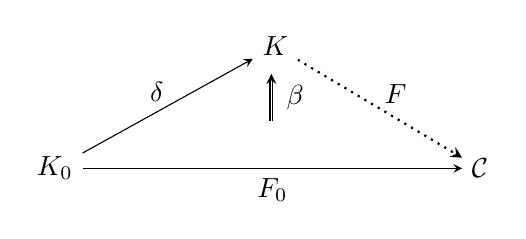
\begin{tikzpicture}[>=stealth]
  \node (K) at (2.8,1.55) {$K$};
  \node (K0) at (0,0) {$K_0$};
  \node (CC) at (5.4,0) {$\cC$};
  \draw[->] (K0) -- (K) node[midway,above left=-2pt] {$\delta$};
  \draw[->,dotted,thick] (K) -- (CC) node[midway,above right=-2pt] {$F$};
  \draw[->] (K0) -- (CC) node[midway,below] {$F_0$};
  \draw[double,->] (2.75,0.6) -- (2.75,1.2) node[midway,right=2pt] {$\beta$};
\end{tikzpicture}
\end{center}
若对任意图 $F'\colon K\to\cC$，
\[
\operatorname{Maps}_{\Fun(K,\cC)}(F,F')\to\operatorname{Maps}_{\Fun(K_0,\cC)}(F\circ\delta,F'\circ\delta)\to\operatorname{Maps}_{\Fun(K_0,\cC)}(F_0,F'\circ\delta)
\]
是 $\infty$-群胚之间的等价，则称 $\beta$ \textbf{展示 $F$ 为 $F_0$ 沿 $\delta$ 的左 Kan 扩张}。

对偶地，给定自然变换 $\beta\colon F\circ\delta\to F_0$，
\begin{center}
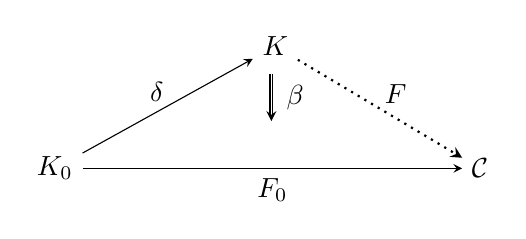
\begin{tikzpicture}[>=stealth]
  \node (K) at (2.8,1.55) {$K$};
  \node (K0) at (0,0) {$K_0$};
  \node (CC) at (5.4,0) {$\cC$};
  \draw[->] (K0) -- (K) node[midway,above left=-2pt] {$\delta$};
  \draw[->,dotted,thick] (K) -- (CC) node[midway,above right=-2pt] {$F$};
  \draw[->] (K0) -- (CC) node[midway,below] {$F_0$};
  \draw[double,->] (2.75,1.2) -- (2.75,0.6) node[midway,right=2pt] {$\beta$};
\end{tikzpicture}
\end{center}
若对任意函子 $F'\colon K\to\cC$，
\begin{equation}\label{L9-eq1.1}
\operatorname{Maps}_{\Fun(K,\cC)}(F',F)\to\operatorname{Maps}_{\Fun(K_0,\cC)}(F'\circ\delta,F\circ\delta)\to\operatorname{Maps}_{\Fun(K_0,\cC)}(F'\circ\delta,F_0)
\end{equation}
是 $\infty$-群胚之间的等价，则称 $\beta$ \textbf{展示 $F$ 为 $F_0$ 沿 $\delta$ 的右 Kan 扩张}。
\end{definition}

\nitem\label{L9-1.3} 可以证明：$\beta$ 展示 $F$ 为 $F_0$ 沿 $\delta$ 的右 Kan 扩张，当且仅当
\begin{equation}\label{L9-eq1.2}
(F,\beta)\in\Fun(K,\cC)\times_{\Fun(K_0,\cC)}\Fun(K_0,\cC)_{/F_0}
\end{equation}
是终对象\footnote{证明梗概：从 $(F',\beta')$ 到 $(F,\beta)$ 的映射空间等价于 \eqref{L9-eq1.1} 在 $\beta'$ 处的同伦纤维。Kan 复形之间的态射是弱同伦等价，当且仅当该态射的每个同伦纤维都弱可缩。}。特别地，这样的对 $(F,\beta)$ 本质唯一。因此，只要把自然变换 $\beta$ 作为其定义的一部分数据，我们就可以谈论 $F_0$ 沿 $\delta$ 的\textbf{右/左 Kan 扩张}。我们把相应的图记为
\[
\mathrm{RKE}_\delta F_0,\qquad \mathrm{LKE}_\delta F_0.
\]
在写 $\mathrm{RKE}_\delta F_0$ 时，我们总把它视为 $\Fun(K,\cC)$ 中的对象，并带有到纤维积 \eqref{L9-eq1.2} 的\textbf{典范}提升。

\nitem\label{L9-1.4} 注意
\[
(\mathrm{LKE}_\delta F_0)^{\op}\simeq\mathrm{RKE}_{\delta^{\op}}F_0^{\op}.
\]
因此下文集中讨论右 Kan 扩张。

\nitem\label{L9-1.5} 与经典范畴论一样，可以证明取伴随函子与复合相容。因此有如下结果。

\begin{proposition}\label{L9-1.6}
设 $K_0\xrightarrow{\delta}K_1\xrightarrow{\theta}K_2$ 是 $\Set_\Delta$ 中的态射，$F_0\colon K_0\to\cC$ 是 $\infty$-范畴 $\cC$ 中的图。假设 $\mathrm{RKE}_\delta F_0$ 存在。则有典范等价
\[
\mathrm{RKE}_\theta(\mathrm{RKE}_\delta F_0)\xrightarrow{\ \simeq\ }\mathrm{RKE}_{\theta\circ\delta}F_0,
\]
其中源存在当且仅当靶存在。
\end{proposition}

\begin{remark}\label{L9-1.7}
上述等价的确切含义如下。设 $\beta\colon F_1\circ\delta\to F_0$ 展示 $F_1$ 为 $F_0$ 沿 $\delta$ 的右 Kan 扩张，$\gamma\colon F_2\circ\theta\to F_1$ 展示 $F_2$ 为 $F_1$ 沿 $\theta$ 的右 Kan 扩张，则
\[
F_2\circ\theta\circ\delta\xrightarrow{\gamma(\delta)}F_1\circ\delta\xrightarrow{\beta}F_0
\]
展示 $F_2$ 为 $F_0$ 沿 $\theta\circ\delta$ 的右 Kan 扩张。
\end{remark}

\begin{theorem}\label{L9-1.8}
设 $\delta\colon K_0\to K$ 是 $\Set_\Delta$ 中的态射，$F_0\colon K_0\to\cC$ 是 $\infty$-范畴 $\cC$ 中的图。假设：
\begin{itemize}[leftmargin=2.2em,itemsep=0.1em]
\item $K$ 是拟范畴；
\item 对任意对象 $x\in K$，图\footnote{纤维积 $K_0\times_K K_{x/}$ 在普通范畴 $\Set_\Delta$ 中取。由于 $K_{x/}\to K$ 是范畴纤维化，它同时也计算 $\Set_\Delta^{\mathrm{Joyal}}$ 中的同伦纤维积。特别地，当 $K_0$ 也是拟范畴时，可以把上述纤维积视为在拟范畴 $\mathrm{QCat}$ 中取。因此，我们可以纯粹用 $\infty$-范畴的语言来陈述上述命题。}
\[
K_0\times_K K_{x/}\xrightarrow{p^x}K_0\xrightarrow{F_0}\cC
\]
的极限存在。
\end{itemize}
则 $\mathrm{RKE}_\delta F_0$ 存在，且有典范同构
\begin{equation}\label{L9-eq1.3}
(\mathrm{RKE}_\delta F_0)(x)\simeq\lim_{K_0\times_K K_{x/}}(F_0\circ p_x).
\end{equation}
\end{theorem}

\begin{definition}\label{L9-1.9}
若 $\delta$ 与 $F_0$ 满足定理~\ref{L9-1.8} 中的假设，则称 $\mathrm{RKE}_\delta F_0$ 是\textbf{点态的}\footnote{并非所有右 Kan 扩张都是点态的。此外，Lurie 定义（见 Ker.02Y9）右 Kan 扩张为 $x\mapsto\lim_{K_0\times_K K_{x/}}(F_0\circ p_x)$，并证明（见 Ker.0309）它满足定义~\ref{L9-1.2} 中的泛性质。因此，Lurie 的右 Kan 扩张应当就是本讲义中的\textbf{点态}右 Kan 扩张。}。
\end{definition}

\begin{remark}\label{L9-1.10}
注意，构造 $x\mapsto K_0\times_K K_{x/}$ 是（反变地）函子性的，而朴素的构造 $x\mapsto K\times_{\cC}\{x\}$ 不是函子性的。
\end{remark}

\begin{remark}\label{L9-1.11}
同构 \eqref{L9-eq1.3} 可以如下非形式地得到。固定函子 $F\colon K\to\cC$ 与自然变换 $\beta\colon F\circ\delta\to F_0$。对对象 $(y,f)\in K_0\times_K K_{x/}$，其中 $y\in K_0$ 而 $f\colon x\to\delta(y)$ 是 $\cC$ 中的态射，考虑复合
\begin{equation}\label{L9-eq1.4}
F(x)\xrightarrow{F(f)}F\circ\delta(y)\xrightarrow{\beta(y)}F_0(y).
\end{equation}
该构造对 $(y,f)$ 是函子性的，因此只要靶存在，就对应一个态射
\begin{equation}\label{L9-eq1.5}
F(x)\to\lim_{(y,f)\in K_0\times_K K_{x/}}F_0(y).
\end{equation}
现在命题断言：\eqref{L9-eq1.5} 对任意 $x$ 可逆，当且仅当 $\beta$ 展示 $F$ 为 $F_0$ 沿 $\delta$ 的右 Kan 扩张。换言之，自然变换 $\beta$ 完全编码在态射 \eqref{L9-eq1.4} 及其高阶函子性之中。
\end{remark}

\begin{remark}\label{L9-1.12}
为把上述构造翻译成同伦连贯的语言，首先注意存在一个显然的自然变换，从常值函子 $\underline{x}\colon K_{x/}\to K$ 到遗忘函子 $\mathrm{oblv}$。与投影函子 $K_0\times_K K_{x/}\to K_{x/}$ 前复合，便得到下图中的左自然变换：
\begin{center}
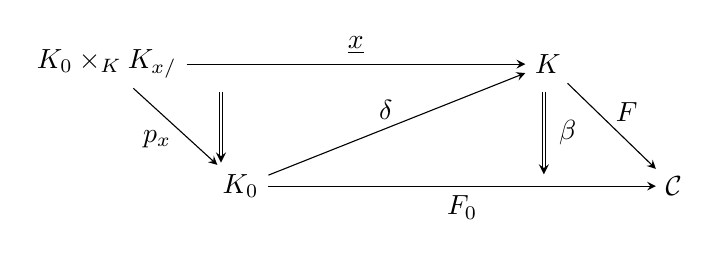
\begin{tikzpicture}[>=stealth]
\node (A) at (0,1.55) {$K_0\times_K K_{x/}$};
\node (K) at (5.6,1.55) {$K$};
\node (K0) at (1.7,0) {$K_0$};
\node (CC) at (7.2,0) {$\cC$};
\draw[->] (A) -- (K) node[midway,above] {$\underline{x}$};
\draw[->] (A) -- (K0) node[midway,below left=-2pt] {$p_x$};
\draw[->] (K0) -- (K) node[midway,above left=-2pt] {$\delta$};
\draw[->] (K0) -- (CC) node[midway,below] {$F_0$};
\draw[->] (K) -- (CC) node[midway,above right=-2pt] {$F$};
\draw[double,->] (1.45,1.2) -- (1.45,0.3);
\draw[double,->] (5.55,1.2) -- (5.55,0.15) node[midway,right=2pt] {$\beta$};
\end{tikzpicture}
\end{center}
与 $\beta$ 复合，得到自然变换 $F(x)\to F_0\circ p_x$；按定义，它对应于 $F(x)$ 沿
\[
\cC^{/F_0\circ p_x}\to\cC
\]
的一个提升，其中源 $\cC^{/F_0\circ p_x}$ 是第 6 讲第 5 节中的另一种切片范畴。现在命题断言：上述提升对任意 $x\in K$ 都是终对象（假定存在），当且仅当 $\beta$ 展示 $F$ 为 $F_0$ 沿 $\delta$ 的右 Kan 扩张。
\end{remark}

\begin{exercise}\label{L9-1.13}
对 $\pi\colon K\to\Delta^0$，证明 $\mathrm{RKE}_\pi u$ 存在当且仅当 $\lim u$ 存在。此外还有
\[
(\mathrm{RKE}_\pi u)(\ast)\simeq\lim u.
\]
如何找出 $(\mathrm{RKE}_\pi u)(\ast)$ 在 $\cC_{/u}$ 中的典范提升？
\end{exercise}

\begin{warning}\label{L9-1.14}
注意，纤维积 $K_0\times_K K_{x/}$ 也出现在 Quillen 定理 A 的陈述中。该定理断言下述两个条件等价：
\begin{enumerate}[label=(\roman*),leftmargin=2.6em,itemsep=0.1em]
\item 态射 $K_0\to K$ 是终的。
\item 对任意 $x\in K$，纤维积 $K_0\times_K K_{x/}$ 弱可缩。
\end{enumerate}
但请注意：(i) 与余极限因而与左 Kan 扩张有关，而定理~\ref{L9-1.8} 与右 Kan 扩张有关。我不知道如何联系这两个结果。
\end{warning}

\begin{exercise}\label{L9-1.15}
证明：右 Kan 扩张 $\mathrm{RKE}_\delta F_0$ 是点态的，当且仅当它被任意可表函子 $\operatorname{Maps}_{\cC}(c,-)\colon\cC\to\Grpd_\infty$ 保持。
\end{exercise}

\begin{proposition}\label{L9-1.16}
设 $\iota\colon K_0\to K$ 是 $\infty$-范畴之间的全忠实函子，$F_0\colon K_0\to\cC$ 是任意函子。假设点态右 Kan 扩张 $\mathrm{RKE}_\iota F_0$ 存在\footnote{这是指该右 Kan 扩张存在并且是点态的。}，则典范自然变换
\[
(\mathrm{RKE}_\iota F_0)\circ\iota\to F_0
\]
可逆。
\end{proposition}

\begin{proof}[证明梗概]
我们只需对任意 $x_0\in K_0$ 与 $x\coloneqq\iota(x_0)$，证明求值态射
\[
\lim_{K_0\times_K K_{x/}}(F_0\circ p_x)\to F_0(x_0)
\]
可逆。而这只需证明 $(x_0,\ x\xrightarrow{=}\iota(x_0))\in K_0\times_K K_{x/}$ 是始对象。这由显然的等价 $(K_0)_{x_0/}\to K_0\times_K K_{x/}$ 推出。
\end{proof}

\begin{exercise}\label{L9-1.17}
对 $\infty$-范畴 $K$，考虑显然的嵌入 $\iota\colon K\to K^{\triangleleft}$。证明：点态右 Kan 扩张 $\mathrm{RKE}_\iota u$ 存在，当且仅当 $u\colon K\to\cC$ 的极限存在。此外，$\mathrm{RKE}_\iota u$ 是延拓 $u$ 的极限图。
\end{exercise}

\begin{exercise}\label{L9-1.18}
证明：任意函子沿 $K^{\triangleleft}\to\Delta^0$ 的点态右 Kan 扩张总存在，且由在该函子于顶元 $\ast\in K^{\triangleleft}$ 处的取值给出。
\end{exercise}

\section{极限与极限交换}

\nitem\label{L9-2.1} 从现在起，$u\colon K_1\times K_2\to\cC$ 是 $\infty$-范畴之间的函子\footnote{事实上，这些结果可以推广到 $K_1$ 与 $K_2$ 是单纯集的情形。不过需要稍作修改构造与陈述。例子见 HTT.5.5.2.3。}。设 $\mathrm{pr}_i\colon K_1\times K_2\to K_i$ 与 $\pi_i\colon K_i\to[0]$ 是投影。

\begin{exercise}\label{L9-2.2}
点态右 Kan 扩张 $\mathrm{RKE}_{\mathrm{pr}_1}u$ 存在，当且仅当对任意 $x\in K_1$，$\lim_{K_2}u(x,-)$ 存在。此外，对任意 $x$，有典范同构
\[
(\mathrm{RKE}_{\mathrm{pr}_1}u)(x)\simeq\lim_{K_2}u(x,-).
\]
\end{exercise}

\nitem\label{L9-2.3} 作为推论，我们得到前几讲所承诺的构造
\[
K_1\to\cC,\qquad x\mapsto\lim_{K_2}u(x,-).
\]
结合命题~\ref{L9-1.6}，便得到\textbf{极限的分配律}。

\yizhu{“极限的分配律”指 $\lim_{K_1\times K_2}u\simeq\lim_{x\in K_1}\lim_{K_2}u(x,-)$，即乘积指标上的极限可以逐个因子计算（见推论~\ref{L9-2.4}）。此处的“分配”只是与环的分配律形式相仿，并非同一概念。\textbf{[来源：I]}}

\begin{corollary}\label{L9-2.4}
假设对任意 $x\in K_1$，$\lim_{K_2}u(x,-)$ 存在。则有典范同构
\[
\lim_{K_1\times K_2}u\xrightarrow{\ \simeq\ }\lim_{x\in K_1}\lim_{K_2}u(x,-).
\]
其中源存在当且仅当靶存在。
\end{corollary}

\begin{corollary}\label{L9-2.5}
假设：
\begin{itemize}[leftmargin=2.2em,itemsep=0.1em]
\item 对任意 $x\in K_1$，$\lim_{K_2}u(x,-)$ 存在；
\item 对任意 $y\in K_2$，$\lim_{K_1}u(-,y)$ 存在。
\end{itemize}
则有典范同构
\[
\lim_{x\in K_1}\lim_{K_2}u(x,-)\simeq\lim_{y\in K_2}\lim_{K_1}u(-,y).
\]
其中左端存在当且仅当右端存在。
\end{corollary}

\nitem\label{L9-2.6} 作为应用，我们得到下述关于 $\infty$-范畴的极限的结果。

\begin{theorem}\label{L9-2.7}
设 $u\colon K\to\Cat_\infty$，$i\mapsto\cC_i$，是 $\infty$-范畴的图。考虑求值函子
\[
\mathrm{ev}_i\colon\lim_{i\in K}\cC_i\to\cC_i.
\]
则有 $\infty$-群胚之间的典范等价
\begin{equation}\label{L9-eq2.1}
\operatorname{Maps}_{\lim_{i\in K}\cC_i}(x,y)\xrightarrow{\ \simeq\ }\lim_{i\in K}\operatorname{Maps}_{\cC_i}(\mathrm{ev}_i(x),\mathrm{ev}_i(y)).
\end{equation}
\end{theorem}

\begin{proof}[证明梗概]
按定义，
\[
\operatorname{Maps}_{\cC}(x,y)\simeq\{x\}\times_{\Fun(\{0\},\cC)}\Fun(\Delta^1,\cC)\times_{\Fun(\{1\},\cC)}\{y\}
\]
可以写成极限。于是定理由推论~\ref{L9-2.5} 以及 $\Fun(J,-)$ 保持极限这一事实推出。
\end{proof}

\begin{remark}\label{L9-2.8}
注意我们还有
\begin{equation}\label{L9-eq2.2}
\left(\lim_{i\in K}\cC_i\right)^{\simeq}\xrightarrow{\ \simeq\ }\lim_{i\in K}\cC_i^{\simeq},
\end{equation}
因为取核心是右伴随。实践中，关于 $\lim_{i\in K}\cC_i$ 的绝大多数（如果不是全部）结果都是用 \eqref{L9-eq2.1} 与 \eqref{L9-eq2.2} 证明的。
\end{remark}

\yizhu{“核心”即 $\infty$-范畴的 $\simeq$-群胚 $(-)^{\simeq}$，由把每个态射都视为可逆得到；勿与 t-结构的心（heart）相混。\textbf{[来源：B]}}

\section{如何使极限与余极限交换？}

\nitem\label{L9-3.1} 为简便起见，假设 $\cC$ 允许 $K_1$-指标的极限与 $K_2$-指标的余极限。特别地，练习~\ref{L9-2.2} 及其对偶蕴含下面所有的 LKE 与 RKE 都存在。

\begin{construction}\label{L9-3.2}
我们有一个显然的交换图
\begin{center}
\begin{tikzcd}[column sep=5.2em,row sep=3.4em]
\Fun(K_1\times K_2,\cC) & \Fun(K_1,\cC) \arrow[l, "-\circ \mathrm{pr}_1"] \\
\Fun(K_2,\cC) \arrow[u, "-\circ \mathrm{pr}_2"] & \Fun([0],\cC) \arrow[l, "-\circ \pi_2"] \arrow[u, "-\circ \pi_1"]
\end{tikzcd}
\end{center}
\end{construction}

与经典范畴论一样，我们可以沿水平方向取左伴随，得到一个自然变换\footnote{我们将在以后的讲中详细解释这一点。}
\begin{equation}\label{L9-eq3.1}
\begin{tikzcd}[column sep=5.2em,row sep=3.4em]
\Fun(K_1\times K_2,\cC) \arrow[rr, "\mathrm{LKE}_{\mathrm{pr}_1}"] \arrow[Rightarrow, from=1-1, to=2-3, shorten <=1.2em, shorten >=1.6em] & & \Fun(K_1,\cC) \\
\Fun(K_2,\cC) \arrow[u, "-\circ \mathrm{pr}_2"] \arrow[rr, "\mathrm{LKE}_{\pi_2}"] & & \Fun([0],\cC) \arrow[u, "-\circ \pi_1"]
\end{tikzcd}
\end{equation}

\begin{lemma}\label{L9-3.3}
自然变换 \eqref{L9-eq3.1} 可逆。
\end{lemma}

\begin{proof}[证明梗概]
设 $x\in K_1$ 是对象，$v\in\Fun(K_2,\cC)$ 是图。我们需要证明
\[
\mathrm{LKE}_{\mathrm{pr}_1}(v\circ\mathrm{pr}_2)(x)\to\mathrm{LKE}_{\pi_2}v(\pi_1(x))
\]
可逆。该态射可以等同于
\[
\colim_{(K_1)_{/x}\times_{K_1}(K_1\times K_2)}v'\to\colim_{K_2}v,
\]
其中 $v'$ 是复合 $(K_1)_{/x}\times_{K_1}(K_1\times K_2)\to K_2\xrightarrow{v}\cC$。因此我们只需证明态射 $(K_1)_{/x}\times_{K_1}(K_1\times K_2)\to K_2$ 是终的，这由 [第 7 讲，命题 3.15] 推出。
\end{proof}

\begin{construction}\label{L9-3.4}
由上述引理，我们有交换图
\begin{center}
\begin{tikzcd}[column sep=5.2em,row sep=3.4em]
\Fun(K_1\times K_2,\cC) \arrow[rr, "\mathrm{LKE}_{\mathrm{pr}_1}"] & & \Fun(K_1,\cC) \\
\Fun(K_2,\cC) \arrow[u, "-\circ \mathrm{pr}_2"] \arrow[rr, "\mathrm{LKE}_{\pi_2}"] & & \Fun([0],\cC) \arrow[u, "-\circ \pi_1"]
\end{tikzcd}
\end{center}
然后可以沿竖直方向取右伴随，得到自然变换
\begin{equation}\label{L9-eq3.2}
\begin{tikzcd}[column sep=5.2em,row sep=3.4em]
\Fun(K_1\times K_2,\cC) \arrow[rr, "\mathrm{LKE}_{\mathrm{pr}_1}"] \arrow[dd, "\mathrm{RKE}_{\mathrm{pr}_2}"'] & & \Fun(K_1,\cC) \arrow[dd, "\mathrm{RKE}_{\pi_1}"] \\
& & \\
\Fun(K_2,\cC) \arrow[rr, "\mathrm{LKE}_{\pi_2}"] \arrow[Rightarrow, from=3-1, to=1-3, "{\alpha}"', shorten <=1.4em, shorten >=1.6em] & & \Fun([0],\cC)
\end{tikzcd}
\end{equation}
特别地，对任意 $u\colon K_1\times K_2\to\cC$，我们得到典范态射
\[
\colim_{y\in K_2}\lim_{K_1}u(-,y)\to\lim_{x\in K_1}\colim_{K_2}u(x,-).
\]
\end{construction}

\begin{definition}\label{L9-3.5}
若 \eqref{L9-eq3.2} 可逆，则称 $\cC$ 中 $K_1$-指标的极限与 $K_2$-指标的余极限\textbf{交换}。
\end{definition}

\nitem\label{L9-3.6} 下一讲我们将解释下述结果。

\begin{theorem}\label{L9-3.7}
在 $\Grpd_\infty$ 中，滤过余极限与有限极限交换。
\end{theorem}

\begin{remark}\label{L9-3.8}
一旦引入了紧生成的 $\infty$-范畴，就容易推出上述定理在任何这样的 $\infty$-范畴中成立。
\end{remark}

\begin{warning}\label{L9-3.9}
滤过或有限指标 $\infty$-范畴的定义是微妙的。例如，有限的普通范畴可能不是有限的 $\infty$-范畴。
\end{warning}

\begin{theorem}\label{L9-3.10}
在 $\Grpd_\infty$ 中，筛余极限与有限积交换。
\end{theorem}

\begin{theorem}\label{L9-3.11}
在 $\Grpd_\infty$ 中，小余极限被基变换保持。
\end{theorem}

\appendixsection{图的分解}

\begin{exercise}\label{L9-A.1}
设 $K$ 是单纯集，$K_1,K_2\subset K$ 是 $K$ 的单纯子集，使得
\[
K_1\sqcup_{K_1\cap K_2}K_2\to K
\]
是同构。设 $u\colon K\to\cC$ 是 $\infty$-范畴中的图。证明有典范同构
\[
\lim_K u\xrightarrow{\ \simeq\ }\lim_{K_1}u\times_{\lim_{K_1\cap K_2}u}\lim_{K_2}u.
\]
其中若靶存在，则源存在。
\end{exercise}

\begin{exercise}\label{L9-A.2}
证明 $x\rightrightarrows y$ 的等化子同构于 $x\times_{x\times y}x$。
\end{exercise}

\begin{exercise}\label{L9-A.3}
设 $K$ 是单纯集，$\mathrm{Sub}(K)$ 是 $K$ 的单纯子集构成的部分序集，视为普通范畴。设 $I\to\mathrm{Sub}(K)$，$i\mapsto K_i$ 是普通范畴之间的函子。求一个充分条件，使得对任意图 $u\colon K\to\cC$，都有典范同构
\[
\lim_K u\xrightarrow{\ \simeq\ }\lim_{i\in I}\lim_{K_i}u.
\]
\end{exercise}

\nitem\label{L9-A.4} \textbf{建议阅读}\quad HTT.4.2.3, Ker.03CY.
}{}
\IfFileExists{chunks/lec10.tex}{% =============================================================================
%  lec10.tex —— 第 10 讲 极限与余极限：交换性（底本 PDF 第 80–87 页）
% =============================================================================
\lecture{10}{极限与余极限：交换性}
\begin{center}\small\color{black!55}（底本 PDF 第 80–87 页）\end{center}

上一讲中，对图 $u\colon K_1\times K_2\to\cC$，我们在假定两侧均存在时构造了典范态射
\[
\colim_{y\in K_2}\lim_{K_1}u(-,y)\to\lim_{x\in K_1}\colim_{K_2}u(x,-).
\]
本讲讨论上述态射可逆的若干情形。

\section{有限图}

\begin{definition}\label{L10-1.1}
若单纯集 $K$ 只有有限多个非退化单形，则称 $K$ 为\textbf{有限的}。

若 $\infty$-范畴 $K$ 可由一个作为有限单纯集的拟范畴表示，则称 $K$ 为\textbf{本质有限的}。
\end{definition}

\nitem\label{L10-1.2} 回忆：我们称普通范畴 $K$ 本质有限，当且仅当 $K$ 中对象的等价类构成的集合与 $K$ 中态射构成的集合都有限。

\begin{exercise}\label{L10-1.3}
设 $K$ 是本质有限的 $\infty$-范畴。证明 $hK$ 是本质有限的普通范畴。
\end{exercise}

\begin{exercise}\label{L10-1.4}
设 $K$ 是普通范畴。若 $K$ 作为 $\infty$-范畴是本质有限的，则它作为普通范畴是本质有限的。
\end{exercise}

\begin{warning}\label{L10-1.5}
逆命题不成立：即便是有限的普通范畴，也可能作为 $\infty$-范畴不是本质有限的。
\end{warning}

\begin{exercise}\label{L10-1.6}
设 $\mathrm{Idem}$ 是由下述条件定义的普通范畴：
\begin{itemize}[leftmargin=2.2em,itemsep=0.1em]
\item 有唯一的对象 $\ast$；
\item $\Hom(\ast,\ast)\coloneqq\{\id,e\}$，其中 $e\circ e=e$。
\end{itemize}
证明 $N_{\bullet}(\mathrm{Idem})$ 不等价于一个有限的拟范畴。
\end{exercise}

\begin{exercise}\label{L10-1.7}
设 $\mathbb{B}(\Z/2\Z)$ 是由下述条件定义的普通范畴：
\begin{itemize}[leftmargin=2.2em,itemsep=0.1em]
\item 有唯一的对象 $\ast$；
\item $\Hom(\ast,\ast)\coloneqq\{\id,f\}$，其中 $f\circ f=\id$。
\end{itemize}
证明 $N_{\bullet}(\mathbb{B}(\Z/2\Z))$ 不等价于一个有限的拟范畴。
\end{exercise}

\nitem\label{L10-1.8} 不过，对有限偏序集而言，上述异常现象不会出现。

\begin{exercise}\label{L10-1.9}
设 $J$ 是有限偏序集，视为普通范畴。证明 $N_{\bullet}(J)$ 是有限单纯集。
\end{exercise}

\begin{proposition}\label{L10-1.10}
（Ker.02NB）对任意单纯集 $K$，存在偏序集 $J$ 与初始态射 $N_{\bullet}(J)\to K$。若 $K$ 有限，则可取 $J$ 有限。
\end{proposition}

\nitem\label{L10-1.11}\textbf{推论—定义}\quad 设 $\cC$ 是 $\infty$-范畴。下列条件等价：
\begin{itemize}[leftmargin=2.2em,itemsep=0.1em]
\item $\cC$ 容许以有限单纯集为指标的极限。
\item $\cC$ 容许以本质有限的 $\infty$-范畴为指标的极限。
\item $\cC$ 容许以有限偏序集为指标的极限。
\end{itemize}
若 $\cC$ 满足上述条件，则称 $\cC$ \textbf{容许有限极限}。

设 $F\colon\cC\to\cD$ 是 $\infty$-范畴之间的函子，且 $\cC$ 容许有限极限。下列条件等价：
\begin{itemize}[leftmargin=2.2em,itemsep=0.1em]
\item $F$ 保持以有限单纯集为指标的极限。
\item $F$ 保持以本质有限的 $\infty$-范畴为指标的极限。
\item $F$ 保持以有限偏序集为指标的极限。
\end{itemize}
若 $F$ 满足上述条件，则称 $F$ 是\textbf{左正合的}。

对偶地，设 $F\colon\cC\to\cD$ 是 $\infty$-范畴之间的函子，且 $\cC$ 容许有限余极限。若 $F$ 保持有限余极限，则称 $F$ 是\textbf{右正合的}。

\begin{warning}\label{L10-1.12}
设 $\cC$ 是容许有限极限的 $\infty$-范畴。它未必容许以有限普通范畴为指标的极限。例如，$\cC$ 可能不是幂等完备的。
\end{warning}

\begin{proposition}\label{L10-1.13}
设 $\cC$ 是 $\infty$-范畴。下列条件等价：
\begin{enumerate}[label=(\roman*),leftmargin=2.4em,itemsep=0.1em]
\item $\cC$ 容许有限极限。
\item $\cC$ 容许纤维积与终对象。
\item $\cC$ 容许有限积与等化子。
\end{enumerate}
对左正合函子，我们也有类似的结果。
\end{proposition}

\begin{proof}[证明梗概]
蕴含 (i)$\Rightarrow$(ii)$\Leftrightarrow$(iii) 是标准的。为证明 (ii)$\Rightarrow$(i)，设 $u\colon K\to\cC$ 是有限图。我们需要证明 $\lim u$ 存在。当 $K=\varnothing$ 时，这就是 $\cC$ 的终对象。若 $K$ 非空，我们可在 $\Set_\Delta$ 中找到推挤方块
\begin{center}
\begin{tikzcd}[column sep=3.2em,row sep=2.8em]
\partial\Delta^n \arrow[r] \arrow[d,"{\subset}"{sloped=false}] & K' \arrow[d,"{\subset}"{sloped=false}] \\
\Delta^n \arrow[r,"{\subset}"{sloped=false}] & K
\end{tikzcd}
\end{center}
注意这同时也是 $\Set^{\mathrm{Joyal}}_\Delta$ 中的同伦推挤方块。由图的分解定理（Ker.03DB），我们有
\[
\lim u\xrightarrow{\ \simeq\ }\lim u|_{K'}\times_{\lim u|_{\partial\Delta^n}}\lim u|_{\Delta^n},
\]
其中若靶存在，则源存在。由归纳，我们归约为证明 $K=\Delta^n$ 时的断言，而这由 $\Delta^0\to\Delta^n$ 是初始态射这一事实得到。
\end{proof}

\nitem\label{L10-1.14} 事实上，对上述论证加以细化便可得：

\begin{proposition}\label{L10-1.15}
（HTT.4.4.2.6, 4.4.3.2）设 $\cC$ 是 $\infty$-范畴。下列条件等价：
\begin{enumerate}[label=(\roman*),leftmargin=2.4em,itemsep=0.1em]
\item $\cC$ 容许小极限。
\item $\cC$ 容许纤维积与小积。
\item $\cC$ 容许小积与等化子。
\end{enumerate}
对保持小极限的函子，我们也有类似的结果。
\end{proposition}

\section{滤过的 $\infty$-范畴}

\begin{definition}\label{L10-2.1}
若任意有限图 $u\colon K\to\cC$ 都能扩张为图 $K^{\triangleright}\to\cC$，则称 $\infty$-范畴 $\cC$ 是\textbf{滤过的}（filtered）。

对偶地，若任意有限图 $u\colon K\to\cC$ 都能扩张为图 $K^{\triangleleft}\to\cC$，则称 $\cC$ 是\textbf{余滤过的}。
\end{definition}

\nitem\label{L10-2.2} 注意 $\cC$ 滤过当且仅当 $\cC^{\op}$ 余滤过。因此下文集中讨论滤过的 $\infty$-范畴。

\begin{exercise}\label{L10-2.3}
滤过性在等价下不变。
\end{exercise}

\nitem\label{L10-2.4} 一个归纳论证（它与命题~\ref{L10-1.13} 的证明类似，但更为精细）给出下述结果：

\begin{lemma}\label{L10-2.5}
（Ker.02Q0）$\infty$-范畴 $\cC$ 滤过，当且仅当任意图 $u\colon\partial\Delta^n\to\cC$（$n\ge 0$\footnote{按定义，$\partial\Delta^0=\varnothing$。}）都能扩张为图 $(\partial\Delta^n)^{\triangleright}\to\cC$。
\end{lemma}

\begin{remark}\label{L10-2.6}
注意 $(\partial\Delta^n)^{\triangleright}\simeq\Lambda^{n+1}_{n+1}$。
\end{remark}

\nitem\label{L10-2.7} 回忆：我们称普通范畴 $\cC$ 滤过，若
\begin{enumerate}[label=(\arabic*),leftmargin=2.4em,itemsep=0.1em,start=0]
\item 它非空。
\item 对任意对象 $x_1,x_2\in\cC$，存在带态射 $x_i\to x$ 的对象 $x$。
\item 对 $\cC$ 中任意图 $x\rightrightarrows y$，存在 $y\to z$，使得两个复合 $x\rightrightarrows y\to z$ 相等。
\end{enumerate}
注意条件 $(i)$ 对应 $K=\partial\Delta^i$ 时的扩张问题。

\begin{proposition}\label{L10-2.8}
（Ker.02PS）$\infty$-范畴 $\cC$ 滤过，当且仅当它满足下述条件：
\begin{enumerate}[label=(\arabic*),leftmargin=2.4em,itemsep=0.1em,start=0]
\item 它非空。
\item 对任意对象 $x_1,x_2\in\cC$，存在带态射 $x_i\to x$ 的对象 $x$。
\item 对 $\cC$ 中任意对象 $x,y$ 与任意图 $\partial\Delta^n\to\operatorname{Maps}(x,y)$（$n\ge 1$），存在态射 $y\to z$，使得复合
\[
\partial\Delta^n\to\operatorname{Maps}(x,y)\to\operatorname{Maps}(x,z)
\]
零伦，即等价于常值图\footnote{练习：对 Kan 复形 $K$，态射 $\partial\Delta^n\to K$ 零伦当且仅当它通过 $\Delta^n$ 分解。}。
\end{enumerate}
\end{proposition}

\begin{remark}\label{L10-2.9}
粗略地说，对 $n\ge 2$，扩张问题
\begin{center}
\begin{tikzcd}[column sep=3.6em,row sep=3.0em]
\partial\Delta^n \arrow[r,"u"] \arrow[d] & \cC \\
\Delta^n \arrow[ur,dotted,-{Latex}] &
\end{tikzcd}
\end{center}
对应于扩张问题
\begin{center}
\begin{tikzcd}[column sep=4.8em,row sep=3.0em]
\partial\Delta^{n-1} \arrow[r] \arrow[d] & \operatorname{Maps}(x,y) \\
\Delta^{n-1} \arrow[ur,dotted,-{Latex}] &
\end{tikzcd}
\end{center}
其中 $x=u(0)$、$y=u(n)$。
\end{remark}

\begin{exercise}\label{L10-2.10}
设 $\cC$ 是滤过的 $\infty$-范畴。证明 $h\cC$ 是滤过的普通范畴。
\end{exercise}

\begin{exercise}\label{L10-2.11}
设 $\cC$ 是普通范畴。证明：$\cC$ 作为普通范畴滤过，当且仅当它作为 $\infty$-范畴滤过。
\end{exercise}

\begin{example}\label{L10-2.12}
若 $\infty$-范畴 $\cC$ 含有终对象，则它滤过。
\end{example}

\begin{example}\label{L10-2.13}
若 $\infty$-范畴 $\cC$ 容许有限余极限，则它滤过。
\end{example}

\begin{exercise}\label{L10-2.14}
范畴 $\mathrm{Idem}$ 滤过。
\end{exercise}

\section{滤过余极限与有限极限}

\begin{theorem}\label{L10-3.1}
（Ker.05XS）设 $\cC$ 是小 $\infty$-范畴。则 $\cC$ 滤过，当且仅当函子
\[
\colim\colon\Fun(\cC,\Grpd_\infty)\to\Grpd_\infty
\]
保持有限极限。
\end{theorem}

\begin{warning}\label{L10-3.2}
若把 $\Grpd_\infty$ 换成一般的 $\infty$-范畴，该结论可能不成立。
\end{warning}

\begin{exercise}\label{L10-3.3}
考虑离散拓扑空间 $\Z$ 及其单点紧化 $\Z\cup\{\infty\}$\footnote{$\Z\cup\{\infty\}$ 的闭子集要么有限，要么包含 $\infty$。}。考虑由 $\Z\cup\{\infty\}$ 的闭子集构成的偏序集 $\cP$。证明 $\cP$ 中的滤过余极限未必与有限极限交换。
\end{exercise}

\begin{corollary}\label{L10-3.4}
设 $F\colon\cC\to\cD$ 是 $\infty$-范畴之间的终结函子。若 $\cC$ 滤过，则 $\cD$ 也滤过。
\end{corollary}

\begin{challenge}\label{L10-3.5}
你能给出上述推论的一个证明而不使用定理~\ref{L10-3.1} 吗？
\end{challenge}

\nitem\label{L10-3.6} 回忆：偏序集 $J$ 称为\textbf{有向的}，若它的任意有限子集都在 $J$ 中有上界。

\begin{proposition}\label{L10-3.7}
（Ker.02QA）设 $\cC$ 是 $\infty$-范畴。下列条件等价：
\begin{itemize}[leftmargin=2.2em,itemsep=0.1em]
\item $\cC$ 滤过。
\item 存在有向偏序集 $J$ 与终结函子 $J\to\cC$。
\end{itemize}
\end{proposition}

\begin{proposition}\label{L10-3.8}
设 $\cC$ 是滤过的 $\infty$-范畴，$u\colon K\to\cC$ 是任意有限图。则遗忘函子 $\cC_{u/}\to\cC$ 终结。
\end{proposition}

\begin{proof}
由 Quillen 定理 A，我们只需证明对任意 $x\in\cC$，$\cC_{u/}\times_\cC\cC_{x/}$ 弱可缩。我们有
\[
\cC_{u/}\times_\cC\cC_{x/}\simeq\cC_{u\sqcup x/},
\]
其中 $u\sqcup x\colon K\sqcup\Delta^0\to\cC$ 是 $u$ 与 $x$ 的不交并。现在断言由下面两个练习推出。
\end{proof}

\begin{exercise}\label{L10-3.9}
滤过的 $\infty$-范畴弱可缩。提示：$K\times\Delta^1\to K^{\triangleright}$。
\end{exercise}

\begin{proposition}\label{L10-3.10}
设 $\cC$ 是 $\infty$-范畴。下列条件等价：
\begin{enumerate}[label=(\roman*),leftmargin=2.4em,itemsep=0.1em]
\item $\cC$ 滤过。
\item 对任意有限图 $u\colon K\to\cC$，$\infty$-范畴 $\cC_{u/}$ 滤过。
\item 对任意有限图 $u\colon K\to\cC$，$\infty$-范畴 $\cC_{u/}$ 弱可缩。
\item 对任意有限 $K\in\Set_\Delta$，对角函子 $\cC\to\Fun(K,\cC)$，$x\mapsto\underline{x}$ 终结。
\end{enumerate}
\end{proposition}

\begin{proof}[证明梗概]
蕴含 (i)$\Rightarrow$(ii)$\Rightarrow$(iii)$\Rightarrow$(i) 留作练习。我们将证明 (ii)$\Leftrightarrow$(iii)。由 Quillen 定理 A，(ii) 等价于：对任意 $u\colon K\to\cC$，纤维积
\[
\cC\times_{\Fun(K,\cC)}\Fun(K,\cC)^{u/}
\]
弱可缩。容易看出上述纤维积等价于 $\cC^{u/}$，这就推出断言。
\end{proof}

\section{筛图}

\begin{definition}\label{L10-4.1}
设 $K$ 是单纯集。若对任意有限集 $I$，对角态射 $K\to K^I$ 终结，则称 $K$ 是\textbf{筛的}（sifted）。

对偶地，若对任意有限集 $I$，对角态射 $K\to K^I$ 初始，则称 $K$ 是\textbf{余筛的}。
\end{definition}

\yizhu{术语 sifted 本义为“筛过的”，此处译作“筛的”，其后简称“筛”；相应地 sifted colimit 译作“筛余极限”，与 filtered（滤过的）相区分。\textbf{[来源：B]}}

\nitem\label{L10-4.2} 注意 $\cC$ 筛当且仅当 $\cC^{\op}$ 余筛。因此下文集中讨论筛的 $\infty$-范畴。

\begin{exercise}\label{L10-4.3}
滤过性在等价下不变。
\end{exercise}

\yizhu{练习 4.3 的原文为“Being filtered is invariant under equivalences”，与练习 2.3 逐字重复；按本节主题（筛性）以及它与练习 2.3 的对应关系，此处原文当作“Being sifted”。译文照录原文。\textbf{[来源：I]}}

\begin{example}\label{L10-4.4}
任意滤过的 $\infty$-范畴都是筛的。
\end{example}

\begin{exercise}\label{L10-4.5}
证明单纯集 $K$ 筛，当且仅当它非空且 $K\to K\times K$ 终结。提示：若 $K\to K\times K$ 是弱同伦等价且 $K\neq\varnothing$，则 $K$ 弱可缩。
\end{exercise}

\begin{corollary}\label{L10-4.6}
$\infty$-范畴 $\cC$ 筛，当且仅当它非空，且对任意一对对象 $x,y\in\cC$，$\cC_{x/}\times_\cC\cC_{y/}$ 弱可缩。
\end{corollary}

\begin{warning}\label{L10-4.7}
在经典范畴论中，普通范畴 $\cC$ 称为筛的，若它非空，且对任意一对对象 $x,y\in\cC$，$\cC_{x/}\times_\cC\cC_{y/}$ 连通。筛的普通范畴作为 $\infty$-范畴可能不筛。
\end{warning}

\begin{exercise}\label{L10-4.8}
设 $\Delta_{\le 1}\subset\Delta$ 是由 $[0]$ 与 $[1]$ 构成的全子范畴。证明 $\Delta_{\le 1}^{\op}$ 作为普通范畴筛，但作为 $\infty$-范畴不筛。
\end{exercise}

\begin{exercise}\label{L10-4.9}
证明 $\Delta^{\op}$ 作为 $\infty$-范畴筛。
\end{exercise}

\begin{definition}\label{L10-4.10}
$\Delta^{\op}$-指标图的余极限称为该图的\textbf{几何实现}。$\Delta$-指标图的极限称为该图的\textbf{全化}。
\end{definition}

\nitem\label{L10-4.11} 众所周知，几何实现与滤过余极限几乎生成全部的筛图。见 §A.10。

\begin{proposition}\label{L10-4.12}
设 $F\colon\cC\to\cD$ 是 $\infty$-范畴之间的终结函子。若 $\cC$ 筛，则 $\cD$ 也筛。
\end{proposition}

\begin{proof}
对任意有限集 $I$，考虑交换图
\begin{center}
\begin{tikzcd}[column sep=3.8em,row sep=3.2em]
\cC \arrow[r,"F"] \arrow[d,"\delta_1"'] & \cD \arrow[d,"\delta_2"] \\
\cC^I \arrow[r,"F^I"'] & \cD^I
\end{tikzcd}
\end{center}
由于 $F$ 终结，$F^I$ 也终结（第 7 讲命题 3.16）。由于 $\cC$ 筛，$\delta_1$ 终结。于是 $\delta_2$ 也终结，如所愿望（第 7 讲练习 3.13）。
\end{proof}

\begin{exercise}\label{L10-4.13}
设 $K$ 是筛的单纯集。设 $\cC$、$\cD$、$\cE$ 是容许 $K$-指标余极限的 $\infty$-范畴，$F\colon\cC\times\cD\to\cE$ 是在每个变量上都保持 $K$-指标余极限的函子\footnote{即对任意 $c\in\cC$ 与 $d\in\cD$，$F(c,-)$ 与 $F(-,d)$ 都保持 $K$-指标余极限。}。证明 $F$ 保持 $K$-指标余极限。
\end{exercise}

\section{筛余极限与有限积}

\begin{theorem}\label{L10-5.1}
（HTT.5.5.8.11, Ker.05XM）设 $\cC$ 是小 $\infty$-范畴。则 $\cC$ 筛，当且仅当函子
\[
\colim\colon\Fun(\cC,\Grpd_\infty)\to\Grpd_\infty
\]
保持有限积。
\end{theorem}

\section{余极限的泛性}

\begin{construction}\label{L10-6.1}
设 $\cC$ 是容许纤维积的 $\infty$-范畴。设 $X\to Y$ 是 $\Grpd_\infty$ 中的函子。与经典范畴论一样，我们有伴随
\begin{equation}\label{L10-6.1eq}
(\Grpd_\infty)_{/X}\rightleftarrows(\Grpd_\infty)_{/Y},
\end{equation}
其中：
\begin{itemize}[leftmargin=2.2em,itemsep=0.1em]
\item 左伴随与遗忘函子相容；
\item 右伴随由 $-\times_Y X$ 给出。
\end{itemize}
\end{construction}

\begin{remark}\label{L10-6.2}
或者，上述右伴随可通过单纯模型范畴 $\Set^{\mathrm{KQ}}_\Delta$ 构造。
\end{remark}

\begin{theorem}\label{L10-6.3}
（Ker.05V5）函子
\[
-\times_Y X\colon(\Grpd_\infty)_{/Y}\to(\Grpd_\infty)_{/X}
\]
保持小余极限。
\end{theorem}

\begin{exercise}\label{L10-6.4}
设 $u\colon K\to\Grpd_\infty$，$i\mapsto X_i$ 是小图，记 $X\coloneqq\colim u$。证明存在典范同构
\[
\colim_{i\in K}(X_i\times_X Y)\simeq Y.
\]
\end{exercise}

\appendixsection{滤过余极限}

\begin{proposition}\label{L10-A.1}
设 $\cC$ 是小滤过普通范畴。则任意余极限图 $\bar u\colon\cC^{\triangleright}\to\Set_\Delta$ 也是 $\Set^{\mathrm{Joyal}}_\Delta$ 中的同伦余极限图。
\end{proposition}

\nitem\label{L10-A.2} 我们介绍命题~\ref{L10-A.1} 的两个应用。第一个应用是 $\infty$-范畴的滤过余极限的一个描述。

\begin{exercise}\label{L10-A.3}
函子 $\mathrm{QCat}\to\Cat_\infty$ 保持小的滤过 $\infty$-余极限。
\end{exercise}

\begin{exercise}\label{L10-A.4}
设 $K$ 是小滤过 $\infty$-范畴，$K\to\Cat_\infty$，$i\mapsto\cC_i$ 是图。证明 $\cC\coloneqq\colim_K\cC_i$ 中的任意对象都等价于某个 $i\in K$、$x\in\cC_i$ 的 $\mathrm{ins}_i(x)$。
\end{exercise}

\begin{exercise}\label{L10-A.5}
设 $K$ 是小滤过 $\infty$-范畴，$K\to\Cat_\infty$，$i\mapsto\cC_i$ 是图。对 $i,j\in K$ 与 $x\in\cC_i$、$y\in\cC_j$，证明
\[
\operatorname{Maps}_\cC(\mathrm{ins}_i(x),\mathrm{ins}_j(y))\xleftarrow{\ \simeq\ }\colim_{k\in K_{(i,j)/}}\operatorname{Maps}_{\cC_k}(x_k,y_k),
\]
其中
\begin{itemize}[leftmargin=2.2em,itemsep=0.1em]
\item $K_{(i,j)/}$ 是关于 $\Delta^0\sqcup\Delta^0\xrightarrow{(i,j)}K$ 的余切片 $\infty$-范畴；
\item 对 $k\in K_{(i,j)/}$，$x_k$ 是 $x$ 在函子 $\cC_i\to\cC_k$ 下的像，$y_k$ 类似。
\end{itemize}
\end{exercise}

\nitem\label{L10-A.6} 第二个应用是把一般的余极限分解为有限余极限的滤过余极限。

\begin{exercise}\label{L10-A.7}
设 $K$ 是任意单纯集。证明 $K$ 的有限单纯子集构成的偏序集 $\mathrm{Fin}(K)$ 滤过，且
\[
K\simeq\hocolim_{J\in\mathrm{Fin}(K)}J.
\]
\end{exercise}

\begin{exercise}\label{L10-A.8}
对任意图 $u\colon K\to\cC$，有典范等价
\[
\colim_{J\in\mathrm{Fin}(K)}\colim_J u|_J\xrightarrow{\ \simeq\ }\colim_K u,
\]
其中右端在左端存在时存在。
\end{exercise}

\begin{corollary}\label{L10-A.9}
$\infty$-范畴 $\cC$ 容许小余极限，当且仅当它容许小的滤过余极限与有限余极限。对这样的 $\cC$，函子 $F\colon\cC\to\cD$ 保持小余极限，当且仅当它保持滤过余极限与有限余极限。
\end{corollary}

\nitem\label{L10-A.10} 上述结果说明
\[
\text{small colimits}=\text{small filtered colimits}+\text{finite colimits}.
\]
事实上，我们还有：
\[
\text{small colimits}=\text{small sifted colimits}+\text{finite coproducts}.
\]
\[
\text{small colimits}=\text{small filtered colimits}+\text{geometric realization}+\text{finite coproducts}.
\]
见 HA.1.3.3.10。

\nitem\label{L10-A.11} \textbf{建议阅读}\quad Ker.03DD.

\appendixsection{余极限的强泛性}

\begin{theorem}\label{L10-B.1}
设 $K\to\Grpd_\infty$，$i\mapsto X_i$ 是小图。考虑 $X\coloneqq\colim_{i\in K}X_i$。则存在典范等价
\begin{equation}\label{L10-B.1eq}
(\Grpd_\infty)_{/X}\to\lim_{i\in K}(\Grpd_\infty)_{/X_i},
\end{equation}
其中每个求值函子是
\[
-\times_X X_i\colon(\Grpd_\infty)_{/X}\to(\Grpd_\infty)_{/X_i}.
\]
\end{theorem}

\begin{exercise}\label{L10-B.2}
利用定理~\ref{L10-6.3} 证明 \eqref{L10-B.1eq} 全忠实。
\end{exercise}

\begin{exercise}\label{L10-B.3}
证明：若把 $\Grpd_\infty$ 换成 $\Set$，定理~\ref{L10-6.3} 仍然成立，但定理~\ref{L10-B.1} 将不成立。
\end{exercise}

\nitem\label{L10-B.4} \textbf{建议阅读}\quad Ker.05SB.
}{}
\IfFileExists{chunks/lec11.tex}{% =============================================================================
%  lec11.tex —— 第 11 讲 Yoneda 引理（底本 PDF 第 88–96 页）
% =============================================================================
\lecture{11}{Yoneda 引理}
\begin{center}\small\color{black!55}（底本 PDF 第 88–96 页）\end{center}

本讲讨论 $\infty$-范畴的 Yoneda 引理。

\section{可表函子}

\begin{definition}\label{L11-1.1}
设 $\cC$ 是 $\infty$-范畴，$F\colon\cC^{\op}\to\Grpd_\infty$ 是函子。若对任意对象 $y$，复合
\begin{equation}\label{L11-eq1.1}
\mathrm{Maps}_{\cC^{\op}}(x,y)\to\mathrm{Maps}_{\Grpd_\infty}(F(x),F(y))\xrightarrow{\ \mathrm{ev}_\eta\ }F(y)
\end{equation}
是 $\infty$-群胚之间的等价，则称对象 $\eta\in F(x)$ 展示 $F$ 被对象 $x\in\cC$ 表示。若这样的 $x$ 与 $\eta$ 存在，则称 $F$ 是\textbf{可表的}。

对偶地，设 $G\colon\cC\to\Grpd_\infty$ 是函子。若对任意对象 $y$，复合
\[
\mathrm{Maps}_{\cC}(x,y)\to\mathrm{Maps}_{\Grpd_\infty}(G(x),G(y))\xrightarrow{\ \mathrm{ev}_\eta\ }G(y)
\]
是 $\infty$-群胚之间的等价，则称对象 $\eta\in G(x)$ 展示 $G$ 被对象 $x\in\cC^{\op}$ 余表示。若这样的 $x$ 与 $\eta$ 存在，则称 $G$ 是\textbf{余可表的}。
\end{definition}

\nitem\label{L11-1.2} 注意，$\eta\in F(x)$ 展示 $F\colon\cC^{\op}\to\Grpd_\infty$ 被 $x\in\cC$ 表示，当且仅当同一对象展示 $F$ 被对应的对象 $x\in\cC^{\op}$ 余表示。因此我们将专注于可表函子。

\begin{remark}\label{L11-1.3}
复合 \eqref{L11-eq1.1} 只定义到同伦为止。但注意，等价在同伦下不变。
\end{remark}

\begin{remark}\label{L11-1.4}
复合 \eqref{L11-eq1.1} 把 $\id_x$ 送到 $\eta\in F(x)$。
\end{remark}

\nitem\label{L11-1.5} 容易看出，定义~\ref{L11-1.1} 在等价下不变。具体地说：
\begin{enumerate}[label=(\arabic*),leftmargin=2.4em,itemsep=0.1em]
\item 设 $\eta_1,\eta_2\in F(x)$ 同构，则 $\eta_1$ 展示 $F$ 被 $x$ 表示，当且仅当 $\eta_2$ 如此。
\item 设 $f\colon x\to x'$ 是同构，则 $\eta\in F(x)$ 展示 $F$ 被 $x$ 表示，当且仅当 $F(f)(\eta)\in F(x')$ 展示 $F$ 被 $x'$ 表示。
\end{enumerate}

\begin{warning}\label{L11-1.6}
可能出现 $\eta_1$ 与 $\eta_2$ 都展示 $F$ 被 $x$ 表示、但彼此不同构的情形。也就是说，若 $\eta_1$ 展示 $F$ 被 $x$ 表示，则任意自同构 $f\colon x\to x$ 都给出一个满足同一性质的对象 $F(f)(\eta_1)$。可以证明：$\eta_1$ 与 $F(f)(\eta_1)$ 同构，当且仅当 $f$ 同伦于 $\id_x$。
\end{warning}

\begin{exercise}\label{L11-1.7}
设 $F\colon\cC^{\op}\to\Grpd_\infty$ 是任意函子。证明：存在函子 $\pi_0F\colon h\cC^{\op}\to\Set$，它在唯一等价的意义下唯一，并使下图交换：
\begin{center}
\begin{tikzcd}[column sep=4.4em,row sep=3em]
\cC^{\op}\arrow[r,"F"]\arrow[d] & \Grpd_\infty\arrow[d,"\pi_0"]\\
h\cC^{\op}\arrow[r,"\pi_0F"'] & \Set
\end{tikzcd}
\end{center}
并证明：若 $F$ 可表，则 $\pi_0F$ 作为普通范畴之间的函子可表。
\end{exercise}

\begin{warning}\label{L11-1.8}
练习~\ref{L11-1.7} 的逆命题不成立。换言之，在定义~\ref{L11-1.1} 中，我们不能把 \eqref{L11-eq1.1} 换成映射
\[
\pi_0\mathrm{Maps}_{\cC^{\op}}(x,y)\to\pi_0\mathrm{Maps}_{\Grpd_\infty}(F(x),F(y))\xrightarrow{\ \mathrm{ev}_\eta\ }\pi_0F(y).
\]
\end{warning}

\begin{exercise}\label{L11-1.9}
考虑取值 $\{\ast\}$ 的常值函子 $F\colon\cC^{\op}\to\Grpd_\infty$。$F(x)$ 中的唯一对象展示 $F$ 被 $x$ 表示，当且仅当 $x$ 在 $\cC$ 中是终对象。但注意，$\pi_0F$ 可表，当且仅当 $h\cC$ 有终对象。
\end{exercise}

\nitem\label{L11-1.10} 然而，我们还有下述结果：

\begin{proposition}\label{L11-1.11}
设 $F\colon\cC^{\op}\to\Grpd_\infty$ 是可表函子。则 $\eta\in F(x)$ 展示 $F$ 被 $x\in\cC$ 表示，当且仅当对任意对象 $y$，$\eta$ 诱导集合之间的双射
\[
\pi_0\mathrm{Maps}_{\cC^{\op}}(x,y)\to\pi_0F(y).
\]
\end{proposition}

\begin{proof}
按假设，存在 $\eta'\in F(x')$ 展示 $F$ 被 $x'$ 表示。于是按定义，对象 $\eta\in F(x)$ 对应 $\cC$ 中的态射 $x'\xleftarrow{\ \alpha\ }x$，使得 $F(x')\to F(x)$ 把 $\eta'$ 送到与 $\eta$ 同构的对象。由此得到交换图
\begin{center}
\begin{tikzcd}[column sep=5.2em,row sep=3em]
\pi_0\mathrm{Maps}_{\cC^{\op}}(x,y)\arrow[r]\arrow[d,"-\circ\alpha"'] & \pi_0F(y)\arrow[d,equal]\\
\pi_0\mathrm{Maps}_{\cC^{\op}}(x',y)\arrow[r,"\simeq"'] & \pi_0F(y).
\end{tikzcd}
\end{center}
展开定义，我们得到：
\begin{center}
\begin{tabular}{ll}
$\eta$ 展示 $F$ 被 $x$ 表示 & $\Leftrightarrow$ $\alpha$ 是 $\cC^{\op}$ 中的同构\\
 & $\Leftrightarrow$ $\alpha$ 是 $h\cC^{\op}$ 中的同构\\
 & $\Leftrightarrow$ 对任意 $y$，左侧竖直映射是双射\\
 & $\Leftrightarrow$ 对任意 $y$，上方的水平映射是双射。
\end{tabular}
\end{center}
\end{proof}

\begin{remark}\label{L11-1.12}
普通范畴 $h\cC$ 自然地（严格地）充实于普通对称幺半范畴 $\hGrpd_\infty$（见第 4 讲第 10 节），至少当 $\cC$ 局部小时如此。把这个 $\hGrpd_\infty$-充实范畴\footnote{警告：在 HTT 中，Lurie 只用 $h\cC$ 记它，这与普通同伦范畴的符号相同。}记为 $\overline{h}\cC$。类似地，可以定义可表的 $\hGrpd_\infty$-充实函子 $\overline{h}\cC^{\op}\to\hGrpd_\infty$ 这一概念。于是按定义即知：函子 $F\colon\cC^{\op}\to\Grpd_\infty$ 可表，当且仅当充实函子 $\overline{h}F$ 可表。
\end{remark}

\section{可表函子作为左 Kan 扩张}

\nitem\label{L11-2.1} 注意，二元组 $(F,\eta)$ 可以看成一个图：
\begin{equation}\label{L11-eq2.1}
\begin{tikzpicture}[>=stealth,baseline=(current bounding box.center)]
\node (D) at (0,0) {$\Delta^0$};
\node (C) at (2.8,2.6) {$\cC^{\op}$};
\node (G) at (6,0) {$\Grpd_\infty$};
\draw[->] (D) -- (C) node[midway,above left=-2pt] {$x$};
\draw[->] (D) -- (G) node[midway,below] {$\{\ast\}$};
\draw[->,dotted] (C) -- (G) node[midway,above right=-2pt] {$F$};
\draw[double,->,dotted] (1.7,0.12) -- (1.7,1.5) node[midway,left=2pt] {$\eta$};
\end{tikzpicture}
\end{equation}

\begin{proposition}\label{L11-2.2}
设 $\cC$ 是 $\infty$-范畴，$(F,\eta)$ 如上。则 $\eta$ 展示 $F$ 被 $x$ 表示，当且仅当
\begin{enumerate}[label=(\roman*),leftmargin=2.6em,itemsep=0.1em]
\item 对每个 $y\in\cC^{\op}$，$\infty$-群胚 $\mathrm{Maps}_{\cC^{\op}}(x,y)$ 本质小；
\item 在 \eqref{L11-eq2.1} 中，$\eta$ 展示 $F$ 为常值函子 $\{\ast\}\colon\Delta^0\to\Grpd_\infty$ 沿 $x\colon\Delta^0\to\cC^{\op}$ 的左 Kan 扩张。
\end{enumerate}
\end{proposition}

\begin{proof}[证明梗概]
首先注意，若 $F$ 被 $x$ 表示，则每个 $\mathrm{Maps}_{\cC^{\op}}(x,y)$ 都等价于 $F(y)\in\Grpd_\infty$，因而本质小。于是我们可以只考虑 (i) 成立的情形。按定义，
\[
(\cC^{\op})_{/y}\times_{\cC^{\op}}\Delta^0\simeq\mathrm{Maps}_{\cC^{\op}}(x,y).
\]
由此
\begin{equation}\label{L11-eq2.2}
(\mathrm{LKE}_x\{\ast\})(y)\simeq\colim_{\mathrm{Maps}_{\cC^{\op}}(x,y)}\{\ast\}\simeq\mathrm{Maps}_{\cC^{\op}}(x,y).
\end{equation}
现在 (ii) 等价于：
\begin{itemize}[leftmargin=2.2em,itemsep=0.1em]
\item 由 $\eta$ 诱导的自然变换 $\mathrm{LKE}_x\{\ast\}\to F$ 可逆。
\end{itemize}
这又等价于
\begin{itemize}[leftmargin=2.2em,itemsep=0.1em]
\item 对任意 $y\in\cC^{\op}$，由 $\eta$ 诱导的态射 $(\mathrm{LKE}_x\{\ast\})(y)\to F(y)$ 可逆。
\end{itemize}
展开定义，上述态射同伦于 \eqref{L11-eq1.1} 与 \eqref{L11-eq2.2} 的复合，这就推出所需断言。
\end{proof}

\begin{corollary}\label{L11-2.3}
设 $\cC$ 是 $\infty$-范畴，$x\in\cC$ 是满足大小条件 (i) 的固定对象。则使 $\eta$ 展示 $F$ 被 $x$ 表示的那些二元组 $(F,\eta\in F(x))$ 本质唯一。
\end{corollary}

\begin{remark}\label{L11-2.4}
上述推论的确切含义如下。二元组 $(F,\eta\in F(x))$ 由下述 $\infty$-范畴的纤维积分类：
\begin{center}
\begin{tikzcd}[column sep=4.8em,row sep=2.8em]
& (\Grpd_\infty)_{\{\ast\}/}\arrow[d] &\\
\Fun(\cC^{\op},\Grpd_\infty)\arrow[r,"\mathrm{ev}_x"'] & \Grpd_\infty
\end{tikzcd}
\end{center}
现在命题断言：该纤维积中由满足可表性条件的二元组构成的全子 $\infty$-范畴等价于 $[0]$。
\end{remark}

\nitem\label{L11-2.5} 由上述推论，在放大 $\Grpd_\infty$ 中对象的大小界之后，只要把对象 $\eta$ 作为其定义的一部分数据纳入，我们就可以谈论由对象 $x\in\cC$ 表示的函子 $\cC^{\op}\to\Grpd_\infty$。我们把这个函子记为 $h_x$。使用这些记号时，我们总把它视为 $\Fun(\cC^{\op},\Grpd_\infty)$ 中的对象，并配以 $h_x(x)$ 中的一个典范对象。由于注~\ref{L11-1.4}，我们常把这个对象记为 $\id_x$。现在命题~\ref{L11-2.2} 可以非形式地写成
\[
h_x\xleftarrow{\ \simeq\ }\mathrm{LKE}_x\{\ast\}.
\]
对偶地，被 $x$ 余表示的函子记为 $h^x$。

\begin{exercise}\label{L11-2.6}
把余可表函子 $h^x$ 描述为左 Kan 扩张。
\end{exercise}

\section{Yoneda 引理}

\begin{theorem}\label{L11-3.1}
设 $\cC$ 是 $\infty$-范畴，$h_x\colon\cC^{\op}\to\Grpd_\infty$ 是被 $x$ 表示的函子。则对任意函子 $G\colon\cC^{\op}\to\Grpd_\infty$，复合
\[
\mathrm{Maps}_{\Fun(\cC^{\op},\Grpd_\infty)}(h_x,G)\to\mathrm{Maps}_{\Grpd_\infty}(h_x(x),G(x))\xrightarrow{\ \mathrm{ev}_{\id_x}\ }G(x)
\]
是 $\infty$-范畴之间的等价。
\end{theorem}

\begin{proof}
通过等价 $h_x\xleftarrow{\ \simeq\ }\mathrm{LKE}_x\{\ast\}$，该复合为
\begin{multline*}
\mathrm{Maps}_{\Fun(\cC^{\op},\Grpd_\infty)}(\mathrm{LKE}_x\{\ast\},G)\to\mathrm{Maps}_{\Fun(\Delta^0,\Grpd_\infty)}((\mathrm{LKE}_x\{\ast\})\big|_{x},G\big|_{x})\\
\to\mathrm{Maps}_{\Fun(\Delta^0,\Grpd_\infty)}(\{\ast\},G\big|_{x})\simeq G(x),
\end{multline*}
由 LKE 的定义，它是等价。
\end{proof}

\begin{exercise}\label{L11-3.2}
证明警告~\ref{L11-1.6} 中的最后一项断言。
\end{exercise}

\nitem\label{L11-3.3} 由命题~\ref{L11-2.2}，函子 $h_x$ 由定理~\ref{L11-2.2} 的结论刻画。事实上，下述更强的结果成立。

\yizhu{原文此处称“定理 2.2”，但第 2 节只有命题 2.2，所指应为命题 2.2；译文照录原文。\textbf{[译者按（无外部依据）]}}

\begin{proposition}\label{L11-3.4}
设 $\cC$ 是 $\infty$-范畴，$x\in\cC$ 是满足大小条件 (i) 的对象。设 $F\colon\cC^{\op}\to\Grpd_\infty$ 是函子，$\eta\in F(x)$。则下列条件等价：
\begin{enumerate}[label=(\arabic*),leftmargin=2.4em,itemsep=0.15em]
\item $\eta$ 展示 $F$ 是被 $x$ 表示的函子；
\item 对任意函子 $G\colon\cC^{\op}\to\Grpd_\infty$，$\eta$ 诱导 $\infty$-范畴之间的等价
\[
\mathrm{Maps}_{\Fun(\cC^{\op},\Grpd_\infty)}(F,G)\to G(x);
\]
\item 对任意函子 $G\colon\cC^{\op}\to\Grpd_\infty$，$\eta$ 诱导集合之间的等价
\[
\pi_0\mathrm{Maps}_{\Fun(\cC^{\op},\Grpd_\infty)}(F,G)\to\pi_0G(x).
\]
\end{enumerate}
\end{proposition}

\begin{proof}
只需证明 (3)$\Rightarrow$(1)。大小假设蕴含 $h_x$ 存在。由定理~\ref{L11-3.1}，存在自然变换 $\alpha\colon h_x\to F$，把 $\id_x\in h_x(x)$ 送到与 $\eta\in F(x)$ 同构的对象。由此得到交换图
\begin{center}
\begin{tikzcd}[column sep=6.2em,row sep=3.2em]
\pi_0\mathrm{Maps}_{\Fun(\cC^{\op},\Grpd_\infty)}(F,G)\arrow[r,"\simeq"]\arrow[d,"-\circ\alpha"'] & \pi_0G(x)\arrow[d,equal]\\
\pi_0\mathrm{Maps}_{\Fun(\cC^{\op},\Grpd_\infty)}(h_x,G)\arrow[r,"\simeq"'] & \pi_0G(x).
\end{tikzcd}
\end{center}
这蕴含 $\alpha$ 是 $h\Fun(\cC^{\op},\Grpd_\infty)$ 中的同构，从而是 $\Fun(\cC^{\op},\Grpd_\infty)$ 中的同构，而这蕴含 (1)。
\end{proof}

\begin{remark}\label{L11-3.5}
在本注中，我们比较命题~\ref{L11-1.11} 与命题~\ref{L11-3.4}。

一旦发展了部分定义的伴随函子的理论，我们就能把定义~\ref{L11-1.1} 与命题~\ref{L11-1.11} 中的条件分别改述为
\begin{enumerate}[label=(\alph*),leftmargin=2.6em,itemsep=0.2em]
\item $\eta$ 展示 $x$ 为 $\{\ast\}\in\Grpd_\infty$ 在函子 $F\colon\cC^{\op}\to\Grpd_\infty$ 的左伴随函子下的可能取值。
\item[(a$'$)] $\eta$ 展示 $x$ 为 $\{\ast\}\in\hGrpd_\infty$ 在函子 $\overline{h}F\colon\overline{h}\cC^{\op}\to\hGrpd_\infty$ 的左伴随函子下的可能取值。
\end{enumerate}
命题~\ref{L11-1.11} 说的是：若 $F$ 的部分定义左伴随在 $\{\ast\}$ 处有定义，则其取值可由同伦范畴检测。

类似地，我们可以把命题~\ref{L11-3.4} 中的 (2) 与 (3) 分别改述为：
\begin{enumerate}[label=(\alph*),leftmargin=2.6em,itemsep=0.2em,start=2]
\item $\eta$ 展示 $F$ 为 $\{\ast\}\in\Grpd_\infty$ 在函子 $\mathrm{ev}_x\colon\Fun(\cC^{\op},\Grpd_\infty)\to\Grpd_\infty$ 的左伴随函子下的可能取值。
\item[(b$'$)] $\eta$ 展示 $F$ 为 $\{\ast\}\in\hGrpd_\infty$ 在函子 $\overline{h}(\mathrm{ev}_x)\colon\overline{h}\Fun(\cC^{\op},\Grpd_\infty)\to\hGrpd_\infty$ 的左伴随函子下的可能取值。
\end{enumerate}
命题~\ref{L11-3.4} 说的是：若 $\mathrm{ev}_x$ 的部分定义左伴随在 $\{\ast\}$ 处有定义，则其取值可由同伦范畴检测。

事实上，对任意函子的部分定义伴随函子，类似的断言都成立。
\end{remark}

\begin{exercise}\label{L11-3.6}
将上述范式应用于 $\infty$-范畴中的终对象。与第 6 讲练习 2.8 比较。
\end{exercise}

\begin{exercise}\label{L11-3.7}
找出下述论证中的错误。
\begin{itemize}[leftmargin=2.2em,itemsep=0.1em]
\item 错误断言：若图 $u\colon K\to\cC$ 的极限存在，则它可以在同伦范畴 $h\cC$ 中计算。
\item 虚假证明：极限可以写成一个 LKE，而 LKE 是某个部分定义左伴随的取值。
\end{itemize}
\end{exercise}

\section{Yoneda 嵌入}

\nitem\label{L11-4.1} 本节给出函子
\[
\mathrm{Maps}_{\cC}(-,-)\colon\cC^{\op}\times\cC\to\Grpd_\infty
\]
的一个构造，方式是经由单纯范畴。在以后的讲次中，我们会利用左纤维化理论给出一个纯拟范畴的构造。

\begin{construction}\label{L11-4.2}
设 $\cC$ 是局部小的\footnote{这意指对任意对象 $x$ 与 $y$，$\mathrm{Maps}_{\cC}(x,y)$ 是小。}拟范畴，并考虑单纯范畴 $\mathbb{C}\coloneqq\mathfrak{C}(\cC)$。设 $\mathbb{C}\to\mathbb{C}'$ 是纤维替换。考虑单纯函子的复合：
\[
\mathfrak{C}(\cC^{\op}\times\cC)\to\mathfrak{C}(\cC^{\op})\times\mathfrak{C}(\cC)\simeq\mathbb{C}^{\op}\times\mathbb{C}\to(\mathbb{C}')^{\op}\times\mathbb{C}'\to\Kan,
\]
其中最后一个函子由 $\Hom_{\mathbb{C}'}(-,-)$ 给出。由伴随性，我们得到函子
\[
\cC^{\op}\times\cC\to N_{\bullet}(\Kan)\eqqcolon\Kan.
\]
\end{construction}

\begin{exercise}\label{L11-4.3}
所得函子 $\cC^{\op}\times\cC\to\Kan$ 的等价类不依赖 $\mathbb{C}'$ 的选取。换言之，我们得到
\[
\pi_0(\Fun(\cC^{\op}\times\cC,\Kan)^{\simeq})
\]
中的一个良定义元素。
\end{exercise}

\begin{exercise}\label{L11-4.4}
上述等价类在 $\cC$ 的等价下不变。换言之，对等价 $\cC\to\cD$，映射
\[
\pi_0(\Fun(\cD^{\op}\times\cD,\Kan)^{\simeq})\to\pi_0(\Fun(\cC^{\op}\times\cC,\Kan)^{\simeq})
\]
保持相应的元素。
\end{exercise}

\nitem\label{L11-4.5} 作为推论，对局部小的 $\infty$-范畴 $\cC$，我们得到函子
\[
\mathrm{Maps}_{\cC}(-,-)\colon\cC^{\op}\times\cC\to\Grpd_\infty,
\]
其等价类不依赖任何选取。

\begin{exercise}\label{L11-4.6}
在相差等价的意义下，上述函子提升第 4 讲第 10 节中构造的函子 $\cC^{\op}\times\cC\to\hGrpd_\infty$。
\end{exercise}

\begin{exercise}\label{L11-4.7}
对任意对象 $x\in\cC$，态射 $f\in\mathrm{Maps}_{\cC}(y,x)$ 展示函子
\[
\mathrm{Maps}_{\cC}(-,x)\colon\cC^{\op}\to\Grpd_\infty
\]
被 $y$ 表示，当且仅当 $f$ 可逆。特别地，态射 $\id_x$ 给出典范等价
\[
\mathrm{Maps}_{\cC}(-,x)\simeq h_x.
\]
对偶地，有典范等价
\[
\mathrm{Maps}_{\cC}(x,-)\simeq h^x.
\]
\end{exercise}

\begin{corollary}\label{L11-4.8}
设 $\cC$ 是局部小的 $\infty$-范畴。函子
\[
\cC\to\Fun(\cC^{\op},\Grpd_\infty),\qquad x\mapsto\mathrm{Maps}_{\cC}(-,x)
\]
全忠实，且其本质像由可表函子组成。
\end{corollary}

\begin{definition}\label{L11-4.9}
设 $\cC$ 是局部小的 $\infty$-范畴。
\begin{itemize}[leftmargin=2.2em,itemsep=0.1em]
\item 一个（协变）\textbf{Yoneda 嵌入}是与 $x\mapsto\mathrm{Maps}_{\cC}(-,x)$ 等价的函子 $\cC\to\Fun(\cC^{\op},\Grpd_\infty)$。
\item 一个（反变）\textbf{Yoneda 嵌入}是与 $x\mapsto\mathrm{Maps}_{\cC}(x,-)$ 等价的函子 $\cC^{\op}\to\Fun(\cC,\Grpd_\infty)$。
\end{itemize}
\end{definition}

\begin{definition}\label{L11-4.10}
设 $\cC$ 是本质小的 $\infty$-范畴。记
\[
\mathrm{PShv}(\cC)\coloneqq\Fun(\cC^{\op},\Grpd_\infty),
\]
并称之为 $\cC$ 上的\textbf{预层 $\infty$-范畴}。
\end{definition}

\begin{remark}\label{L11-4.11}
在上述定义中，我们要求 $\cC$ 本质小而非局部小，以保证 $\mathrm{PShv}(\cC)$ 局部小。但注意，$\mathrm{PShv}(\cC)$ 几乎从不是小的。
\end{remark}

\nitem\label{L11-4.12} 设 $\cC$ 是本质小的 $\infty$-范畴。回忆 $\mathrm{PShv}(\cC)\coloneqq\Fun(\cC^{\op},\Grpd_\infty)$ 具有所有小极限与小余极限，且可以逐点计算（第 7 讲定理 2.14）。

下述结果等价于第 7 讲定理 2.11。用单纯范畴的证明见 HTT.5.1.3.2。

\begin{theorem}\label{L11-4.13}
设 $\cC$ 是本质小的 $\infty$-范畴。则 Yoneda 嵌入 $\cC\to\mathrm{PShv}(\cC)$ 保持并检测所有极限。
\end{theorem}

\begin{warning}\label{L11-4.14}
小图 $u\colon K\to\cC$ 的极限可能不存在。这发生当且仅当 $K\to\cC\to\mathrm{PShv}(\cC)$ 的极限不是可表预层。
\end{warning}

\section{余完备化}

\begin{definition}\label{L11-5.1}
设 $\cC$ 是 $\infty$-范畴。若下述条件成立，则称函子 $\cC\to\widehat{\cC}$ 展示 $\widehat{\cC}$ 为 $\cC$ 的\textbf{余完备化}：
\begin{itemize}[leftmargin=2.2em,itemsep=0.1em]
\item $\infty$-范畴 $\widehat{\cC}$ 具有小余极限；
\item 对任意具有小余极限的 $\infty$-范畴 $\cD$，限制函子
\[
\mathrm{LFun}(\widehat{\cC},\cD)\to\Fun(\cC,\cD)
\]
是等价，其中 $\mathrm{LFun}(\widehat{\cC},\cD)\subset\Fun(\widehat{\cC},\cD)$ 是由保持小余极限的函子构成的全子 $\infty$-范畴。
\end{itemize}
\end{definition}

\begin{theorem}[Ker.04BE]\label{L11-5.2}
设 $\cC$ 是本质小的 $\infty$-范畴。Yoneda 嵌入 $\iota\colon\cC\to\mathrm{PShv}(\cC)$ 展示 $\mathrm{PShv}(\cC)$ 为 $\cC$ 的余完备化。
\end{theorem}

\begin{proof}[证明思路]
我们只需证明限制函子
\begin{equation}\label{L11-eq5.1}
-\circ\iota\colon\mathrm{LFun}(\mathrm{PShv}(\cC),\cD)\to\Fun(\cC,\cD)
\end{equation}
是等价。我们断言 $\mathrm{LKE}_\iota$ 存在，并诱导函子
\begin{equation}\label{L11-eq5.2}
\mathrm{LKE}_\iota\colon\Fun(\cC,\cD)\to\mathrm{LFun}(\mathrm{PShv}(\cC),\cD),
\end{equation}
它与上述限制函子互逆。

事实上，对任意 $F\colon\cC\to\cD$，逐点 LKE $\mathrm{LKE}_\iota F\colon\mathrm{PShv}(\cC)\to\cD$ 存在，因为
\begin{equation}\label{L11-eq5.3}
\cC_{/M}\coloneqq\mathrm{PShv}(\cC)_{/M}\times_{\mathrm{PShv}(\cC)}\cC
\end{equation}
本质小\footnote{正是在这一步，我们用到 $\cC$ 本质小而不只是局部小（Ker.03WG）。在后者这一更弱的假设下，该定理会失效（Ker.03WF）。}，从而
\[
(\mathrm{LKE}_\iota F)(M)\simeq\colim_{(h_x\to M)\in\cC_{/M}}F(x).
\]
可以证明 $\cC_{/\colim M_i}\simeq\colim\cC_{/M_i}$，并利用图的分解证明函子 $\mathrm{LKE}_\iota F$ 保持小余极限。

剩下要证明所得函子 \eqref{L11-eq5.2} 是 \eqref{L11-eq5.1} 的逆。它是右逆，因为 $\iota$ 全忠实。为证明它是左逆，我们需要证明任意保持余极限的 $G\colon\mathrm{PShv}(\cC)\to\cD$ 满足
\begin{equation}\label{L11-eq5.4}
\mathrm{LKE}_\iota(G\circ\iota)\xrightarrow{\ \simeq\ }G.
\end{equation}
\end{proof}

由于 $G$ 保持余极限，且上述 LKE 是逐点的，我们只需处理 $G=\mathrm{Id}$ 的万有情形。由于 $\mathrm{PShv}(\cC)$ 中的小余极限被 $h^{\op}_{\cM}\colon\mathrm{PShv}(\cC)\to\Grpd^{\op}_\infty$ 保持并检测，我们只需处理 $G=h^{\op}_{\cM}$ 的情形。

换言之，我们需要证明交换图
\begin{center}
\begin{tikzcd}[column sep=5.2em,row sep=3.4em]
& \mathrm{PShv}(\cC)^{\op}\arrow[dr,dotted,"h_{\cM}"] &\\
\cC^{\op}\arrow[ur,"\iota^{\op}"]\arrow[rr,"\cM"'] & & \Grpd_\infty
\end{tikzcd}
\end{center}
诱导出
\[
h_{\cM}\xrightarrow{\ \simeq\ }\mathrm{RKE}_{\iota^{\op}}\cM.
\]
这里等价 $\cM\simeq h_{\cM}\circ\iota^{\op}$ 来自 $\cC$ 的 Yoneda 引理。我们只需对任意 $N\in\mathrm{PShv}(\cC)^{\op}$ 证明
\[
h_{\cM}(N)\xrightarrow{\ \simeq\ }(\mathrm{RKE}_{\iota^{\op}}\cM)(N).
\]
对 $\mathrm{PShv}(\cC)$ 应用 Yoneda 引理，我们只需证明\footnote{奇迹就发生在这里。在一般情形下，要检验函子 $T\colon\cU^{\op}\to\cV$ 是 $\cU_0^{\op}\to\cV$ 的 RKE，需要用\emph{所有}函子 $S\colon\cU^{\op}\to\cV$ 作为检验函子并计算 $\mathrm{Maps}(S,T)$。然而当 $\cV=\Grpd_\infty$ 时，上述论证说明只需用可表函子作为检验函子。}
\[
h_{\cM}(N)\xrightarrow{\ \simeq\ }\mathrm{Maps}(h_N,\mathrm{RKE}_{\iota^{\op}}\cM).
\]
展开定义，该函子可以等同于
\[
h_{\cM}(N)\simeq\mathrm{Maps}(N,\cM)\simeq\mathrm{Maps}(h_N\circ\iota^{\op},\cM)\simeq\mathrm{Maps}(h_N,\mathrm{RKE}_{\iota^{\op}}\cM),
\]
其中最后一个等价用到 RKE 的泛性质。

\nitem\label{L11-5.3} 在上述证明中，我们实际上证明了：

\begin{corollary}\label{L11-5.4}
设 $\cC$ 是本质小的 $\infty$-范畴。则 $\mathrm{PShv}(\cC)$ 由 $\iota\colon\cC\to\mathrm{PShv}(\cC)$ 的像在小余极限下生成。
\end{corollary}

\begin{remark}\label{L11-5.5}
上述推论的确切含义是：$\mathrm{PShv}(\cC)$ 中任意对象 $M\in\mathrm{PShv}(\cC)$ 都同构于 $\iota$ 的像中对象的小余极限。事实上，对 $G\coloneqq\mathrm{Id}$ 应用 \eqref{L11-eq5.4}，我们有
\[
M\simeq\colim_{(h_x\to M)\in\cC_{/M}}\iota(x).
\]
\end{remark}

\appendixsection{完全紧对象}

\begin{definition}\label{L11-A.1}
设 $\cD$ 是局部小且具有小余极限的 $\infty$-范畴。若函子
\[
\mathrm{Maps}_{\cD}(d,-)\colon\cD\to\Grpd_\infty
\]
保持小余极限，则称对象 $d\in\cD$ 是\textbf{完全紧的}。
\end{definition}

\yizhu{“完全紧”比第 13 讲的“紧对象”更强：后者只要求 $\mathrm{Maps}_{\cD}(d,-)$ 保持小滤过余极限（第 13 讲定义 2.1），而完全紧要求它保持一切小余极限。\textbf{[来源：B]}}

\begin{exercise}\label{L11-A.2}
设 $d$ 在 $\cD$ 中完全紧。证明 $d$ 的任意收缩也完全紧。这里回忆，若 $\id_c$ 分解为 $c\to d\to c$，则称 $c$ 是 $d$ 的\textbf{收缩}。
\end{exercise}

\begin{exercise}\label{L11-A.3}
设 $\cC$ 是本质小的 $\infty$-范畴。证明可表预层 $h_x\in\mathrm{PShv}(\cC)$ 是完全紧的。
\end{exercise}

\begin{theorem}[HTT.5.1.6.8]\label{L11-A.4}
设 $\cC$ 是本质小的 $\infty$-范畴。则预层 $M\in\mathrm{PShv}(\cC)$ 完全紧，当且仅当它是某个可表预层的收缩。
\end{theorem}

\nitem\label{L11-A.5} \textbf{建议阅读}\quad HTT.5.1.6.
}{}
\IfFileExists{chunks/lec12.tex}{% =============================================================================
%  lec12.tex —— 第 12 讲 伴随函子（底本 PDF 第 97–103 页）
% =============================================================================
\lecture{12}{伴随函子}
\begin{center}\small\color{black!55}（底本 PDF 第 97–103 页）\end{center}

本讲介绍 $\infty$-范畴之间的伴随函子。

\section{定义}

\nitem\label{L12-1.1} 回忆普通范畴论中的下述定义。

\begin{definition}\label{L12-1.2}
设 $F\colon\cC\rightleftarrows\cD:G$ 是普通范畴之间的函子。$F$ 与 $G$ 之间的一个\textbf{伴随}（adjunction）是一族双射
\[
\rho_{x,y}\colon\Hom_{\cD}(F(x),y)\xrightarrow{\ \simeq\ }\Hom_{\cC}(x,G(y)),
\]
它们对 $x\in\cC^{\op}$ 与 $y\in\cD$ 具有函子性。我们也说构造 $(x,y)\mapsto\rho_{x,y}$ \textbf{展示 $F$ 为 $G$ 的左伴随}。
\end{definition}

\nitem\label{L12-1.3} 对偶地，我们也说 $(x,y)\mapsto\rho_{x,y}$ \textbf{展示 $G$ 为 $F$ 的右伴随}。

\nitem\label{L12-1.4} 上文中，双射 $\rho_{x,y}$ 可以编码为下图从顺时针弧到逆时针弧的可逆自然变换：
\[
\begin{tikzcd}[column sep=4.2em,row sep=3.2em]
\cC^{\op}\times\cD \arrow[r,"{(F^{\op},\id)}"] \arrow[d,"{(\id,G)}"'] & \cD^{\op}\times\cD \arrow[d,"{\Hom_{\cD}(-,-)}"] \\
\cC^{\op}\times\cC \arrow[r,"{\Hom_{\cC}(-,-)}"'] & \Set.
\end{tikzcd}
\]
但请注意，在 $\infty$-范畴的情形，函子 $\operatorname{Maps}_{\cC}(-,-)\colon\cC^{\op}\times\cC\to\Grpd_{\infty}$ 的构造要复杂得多。因此我们宁愿用另一种方式来编码 $\rho_{\bullet,\bullet}$。

\begin{definition}\label{L12-1.5}
设 $F\colon\cC\rightleftarrows\cD:G$ 是 $\infty$-范畴之间的函子。
\begin{enumerate}[label=(\arabic*),leftmargin=2.4em,itemsep=0.4em]
\item 设 $\mu\colon\id_{\cC}\to G\circ F$ 是自然变换。若对任意对象 $x\in\cC$ 与 $y\in\cD$，复合
\begin{equation}\label{L12-eq1.1}
\operatorname{Maps}_{\cD}(F(x),y)\xrightarrow{G(-)}\operatorname{Maps}_{\cC}(G\circ F(x),G(y))\xrightarrow{-\circ\mu(x)}\operatorname{Maps}_{\cC}(x,G(y))
\end{equation}
可逆，则称 $\mu$ \textbf{展示 $F$ 为 $G$ 的左伴随}。
\item 设 $\kappa\colon F\circ G\to\id_{\cD}$ 是自然变换。若对任意对象 $x\in\cC$ 与 $y\in\cD$，复合
\begin{equation}\label{L12-eq1.2}
\operatorname{Maps}_{\cC}(x,G(y))\xrightarrow{F(-)}\operatorname{Maps}_{\cD}(F(x),F\circ G(y))\xrightarrow{\kappa(y)\circ-}\operatorname{Maps}_{\cD}(F(x),y)
\end{equation}
可逆，则称 $\kappa$ \textbf{展示 $F$ 为 $G$ 的左伴随}。
\end{enumerate}
\end{definition}

\begin{definition}\label{L12-1.6}
设 $F\colon\cC\rightleftarrows\cD:G$ 是 $\infty$-范畴之间的函子。若一对自然变换 $\mu\colon\id_{\cC}\to G\circ F$ 与 $\kappa\colon F\circ G\to\id_{\cD}$ 满足下述两个条件，则称它们\textbf{在同伦意义下相容}（compatible up to homotopy）：
\begin{enumerate}[label=(\roman*),leftmargin=2.6em,itemsep=0.3em]
\item 复合
\[
F\xrightarrow{\id_F\circ\mu}F\circ G\circ F\xrightarrow{\kappa\circ\id_F}F
\]
在 $\Fun(\cC,\cD)$ 中同伦于 $\id_F$。
\item 复合
\[
G\xrightarrow{\mu\circ\id_G}G\circ F\circ G\xrightarrow{\id_G\circ\kappa}G
\]
在 $\Fun(\cC,\cD)$ 中同伦于 $\id_F$。
\end{enumerate}
\end{definition}

\yizhu{条件 (ii) 中的复合是 $G\to G$，原文却写作“在 $\Fun(\cC,\cD)$ 中同伦于 $\id_F$”。按上下文，此处应为“在 $\Fun(\cD,\cD)$ 中同伦于 $\id_G$”。译文照录原文。\textbf{[译者按（无外部依据）]}}

\begin{warning}\label{L12-1.7}
上述定义中，我们\textbf{并不}提供 2-单形
\[
\begin{tikzcd}[column sep=2.8em,row sep=2.4em]
& F\circ G\circ F \arrow[dl,"\id\circ\mu"'] \arrow[dr,"\kappa\circ\id"] & \\
F \arrow[rr, Rightarrow] & & F
\end{tikzcd}
\qquad
\begin{tikzcd}[column sep=2.8em,row sep=2.4em]
& G\circ F\circ G \arrow[dl,"\mu\circ\id"'] \arrow[dr,"\id\circ\kappa"] & \\
G \arrow[rr, Rightarrow] & & G
\end{tikzcd}
\]
来见证这些同伦。
\end{warning}

\begin{definition}\label{L12-1.8}
我们说：
\begin{enumerate}[label=(\arabic*),leftmargin=2.4em,itemsep=0.2em]
\item 设 $\mu$ 是上面的自然变换。若存在与它同伦相容的 $\kappa$，则称 $\mu$ 是 $F$ 与 $G$ 之间伴随的\textbf{单位}（unit）。
\item 设 $\kappa$ 是上面的自然变换。若存在与它同伦相容的 $\mu$，则称 $\kappa$ 是 $F$ 与 $G$ 之间伴随的\textbf{余单位}（counit）。
\end{enumerate}
\end{definition}

\begin{proposition}\label{L12-1.9}（Ker.02FX）
设 $F\colon\cC\rightleftarrows\cD:G$ 是 $\infty$-范畴之间的函子，$\mu\colon\id_{\cC}\to G\circ F$ 是自然变换。则下述条件等价：
\begin{itemize}[leftmargin=2.2em,itemsep=0.1em]
\item $\mu$ 是 $F$ 与 $G$ 之间伴随的单位。
\item $\mu$ 展示 $F$ 为 $G$ 的左伴随。
\end{itemize}
对偶地，对 $\kappa\colon F\circ G\to\id_{\cD}$，下述条件等价：
\begin{itemize}[leftmargin=2.2em,itemsep=0.1em]
\item $\kappa$ 是 $F$ 与 $G$ 之间伴随的余单位。
\item $\kappa$ 展示 $F$ 为 $G$ 的左伴随。
\end{itemize}
\end{proposition}

\begin{remark}\label{L12-1.10}
$\Rightarrow$ 方向很容易。假设 $(\mu,\kappa)$ 同伦相容，则我们有下述交换图：
\[
\begin{tikzcd}[column sep=3.2em,row sep=2.8em]
{[Fx,y]} \arrow[r,"G"] \arrow[d,equal] & {[GFx,Gy]} \arrow[r,"-\circ\mu(x)"] \arrow[d,"F"] & {[x,Gy]} \arrow[d,"F"] \\
{[Fx,y]} \arrow[r,"FG"] \arrow[d,"\id_{\cD}"'] & {[FGFx,FGy]} \arrow[r,"-\circ\mu(Fx)"] \arrow[d,"\kappa(y)\circ-"] & {[Fx,FGy]} \arrow[d,"\kappa(y)\circ-"] \\
{[Fx,y]} \arrow[r,"-\circ\kappa(Fx)"'] & {[FGFx,y]} \arrow[r,"-\circ\mu(Fx)"'] & {[Fx,y].}
\end{tikzcd}
\]
现在定义~\ref{L12-1.6} 中的公理 (i) 说明底部的水平复合同伦于恒等函子。由此可知，顶部水平函子与右侧竖直函子的复合，即 $\eqref{L12-eq1.2}\circ\eqref{L12-eq1.1}$，同伦于恒等函子。对偶地，公理 (ii) 说明 $\eqref{L12-eq1.1}\circ\eqref{L12-eq1.2}$ 同伦于恒等函子。因此 \eqref{L12-eq1.1} 与 \eqref{L12-eq1.2} 都可逆。

$\Leftarrow$ 方向可以这样证明：只要能为 (1.6) 指定一个足够函子性的逆，以诱导出自然变换 $\kappa$。
\end{remark}

\yizhu{本节只有 \eqref{L12-eq1.1} 与 \eqref{L12-eq1.2} 两个编号公式，原文此处引用的 (1.6) 并不存在；按上下文，它应指 \eqref{L12-eq1.1}。译文照录原文。\textbf{[译者按（无外部依据）]}}

\nitem\label{L12-1.11} \textbf{推论—定义}\quad 设 $F\colon\cC\to\cD$ 是 $\infty$-范畴之间的函子。下述条件等价：
\begin{itemize}[leftmargin=2.2em,itemsep=0.1em]
\item 存在 $G\colon\cD\to\cC$ 与 $\mu\colon\id_{\cC}\to G\circ F$，使得 $\mu$ 展示 $G$ 为 $F$ 的右伴随。
\item 存在 $G\colon\cD\to\cC$ 与 $\kappa\colon F\circ G\to\id_{\cD}$，使得 $\kappa$ 展示 $G$ 为 $F$ 的右伴随。
\item 存在 $G\colon\cD\to\cC$ 以及如上的一对 $(\mu,\kappa)$，它在同伦意义下相容。
\end{itemize}
若 $F$ 满足上述条件，则说 $F$ \textbf{有右伴随}，或称 $F$ \textbf{右可伴随}。对偶地，我们定义\textbf{左可伴随}函子的概念。

\nitem\label{L12-1.12} 实践中，伴随数据（adjunction datum）更适于形式证明。下述练习给出一个例子。

\begin{exercise}\label{L12-1.13}
设 $F\colon\cC\rightleftarrows\cD:G$ 是由其单位或余单位展示的伴随。设 $\cE$ 是任意 $\infty$-范畴，证明：
\begin{enumerate}[label=(\arabic*),leftmargin=2.4em,itemsep=0.2em]
\item 我们有伴随
\[
F\circ-\colon\Fun(\cE,\cC)\rightleftarrows\Fun(\cE,\cD):G\circ-,
\]
它由同一类型的数据展示。
\item 我们有伴随
\[
-\circ G\colon\Fun(\cD,\cE)\rightleftarrows\Fun(\cC,\cE):-\circ F,
\]
它由同一类型的数据展示。
\end{enumerate}
\end{exercise}

\section{可伴随性判据}

\begin{proposition}\label{L12-2.1}
我们有：
\begin{enumerate}[label=(\arabic*),leftmargin=2.4em,itemsep=0.2em]
\item 若 $G\colon\cD\to\cC$ 有左伴随，则 $G$ 保持 $\cD$ 中存在的所有小极限。
\item 若 $F\colon\cC\to\cD$ 有右伴随，则 $F$ 保持 $\cD$ 中存在的所有小余极限。
\end{enumerate}
\end{proposition}

\yizhu{第 (2) 条中的“$\cD$ 中”按对偶应作“$\cC$ 中”，因为 $F$ 的定义域是 $\cC$。译文照录原文。\textbf{[译者按（无外部依据）]}}

\begin{proof}[证明梗概]
我们可以假定 $\cC$ 与 $\cD$ 都是本质小的。则
\[
\begin{aligned}
\operatorname{Maps}_{\cC}(x,G(\lim y_i))&\simeq\operatorname{Maps}_{\cD}(F(x),\lim y_i)\simeq\lim\operatorname{Maps}_{\cD}(F(x),y_i)\simeq\\
&\simeq\lim\operatorname{Maps}_{\cD}(x,G(y_i))\simeq\operatorname{Maps}_{\cD}(x,\lim G(y_i)).
\end{aligned}
\]
这表明 $G(\lim y_i)\simeq\lim G(y_i)$。
\end{proof}

\begin{exercise}\label{L12-2.2}
把上述梗概改写为严格的证明。
\end{exercise}

\begin{remark}\label{L12-2.3}
在以后的讲次中，我们会看到：若 $\cC$ 与 $\cD$ 可表现，则该命题的逆命题成立。
\end{remark}

\begin{proposition}\label{L12-2.4}
设 $G\colon\cD\to\cC$ 是 $\infty$-范畴之间的函子。下述条件等价：
\begin{enumerate}[label=(\roman*),leftmargin=2.6em,itemsep=0.2em]
\item 函子 $G$ 有左伴随。
\item 对任意 $x\in\cC$，函子 $\operatorname{Maps}_{\cC}(x,G(-))\colon\cD\to\Grpd_{\infty}$ 余可表示\footnote{我们选取 $\Grpd_{\infty}$ 中对象的大小界，使得 $\cC$ 与 $\cD$ 相对于它是局部小的。}。
\item 对任意 $x\in\cC$，纤维积 $\cD\times_{\cC}\cC_{x/}$ 有始对象。
\end{enumerate}
此外，在这些条件下，逐点的 $\mathrm{RKE}_{G}\id_{\cD}$ 存在，且
\[
\begin{tikzcd}[column sep=5em,row sep=3.4em]
& \cC \arrow[dl,"G"'] \arrow[dr,dotted,"F"] \arrow[d,dotted,Rightarrow,"{\kappa}"'] & \\
\cD \arrow[rr,"\id_{\cD}"'] & \phantom{\cD} & \cD
\end{tikzcd}
\]
展示 $F$ 为该 RKE，当且仅当它展示 $F$ 为 $G$ 的左伴随。
\end{proposition}

\begin{proof}[证明梗概]
(i)$\Rightarrow$(ii)：设 $F$ 是由 $\mu\colon\id_{\cC}\to G\circ F$ 展示的 $G$ 的左伴随。则 $\mu(x)\in\operatorname{Maps}_{\cC}(x,G\circ F(x))$ 展示 $\operatorname{Maps}_{\cC}(x,G(-))$ 由 $F(x)$ 余表示。

(ii)$\Rightarrow$(iii)：设 $e\in\operatorname{Maps}_{\cC}(x,G(y))$ 展示 $\operatorname{Maps}_{\cC}(x,G(-))$ 由 $y$ 余表示。则 $(y,e)$ 是 $\cD\times_{\cC}\cC_{x/}$ 中的始对象。

（然后可以验证 $\mathrm{RKE}_{G}\id_{\cD}$ 确实是 $G$ 的左伴随。）
\end{proof}

\begin{exercise}\label{L12-2.5}
补全上述梗概的细节。
\end{exercise}

\begin{exercise}\label{L12-2.6}
叙述上述命题的对偶版本。
\end{exercise}

\begin{warning}\label{L12-2.7}
逐点 $\mathrm{RKE}_{G}\id_{\cD}$ 的存在性并不蕴涵 $G$ 的左伴随存在。
\end{warning}

\begin{exercise}\label{L12-2.8}
设 $G\colon\cD\to\cC$ 是任意函子，其中 $\cD\defeq[0]$。证明 $\mathrm{RKE}_{G}\id_{\cD}$ 总存在，而 $G$ 有左伴随当且仅当 $G$ 是终的。
\end{exercise}

\begin{exercise}\label{L12-2.9}
设 $F\colon\cC\rightleftarrows\cD:G$ 是 $\infty$-范畴之间的函子，并考虑同伦范畴之间诱导的函子 $hF\colon h\cC\rightleftarrows h\cD:hG$。假设 $G$ 左可伴随。证明：$\mu$（相应地，$\kappa$）展示 $F$ 为 $G$ 的左伴随，当且仅当 $h\mu$（相应地，$h\kappa$）展示 $hF$ 为 $hG$ 的左伴随。
\end{exercise}

\begin{exercise}\label{L12-2.10}
设 $G\colon\cD\to\cC$ 是 $\infty$-范畴之间的函子。证明：$x\in\cC$ 满足命题~\ref{L12-2.4} 中的 (ii)，当且仅当它满足其中的 (iii)。
\end{exercise}

\begin{exercise}\label{L12-2.11}
上文中，设 $\cC_0\subset\cC$ 是由这些对象构成的全子 $\infty$-范畴。\textbf{挑战：}构造函子 $F_0\colon\cC_0\to\cD$，使得 $F_0(x)$ 余表示 $\operatorname{Maps}_{\cC}(x,G(-))$。
\end{exercise}

\begin{exercise}\label{L12-2.12}
设 $G\colon\cD\to\cC$ 是 $\infty$-范畴之间的函子，$\iota\colon\cC_0\to\cC$ 是全忠实函子。为下述概念找出正确的定义：自然变换 $\mu_0\colon\iota\to G\circ F_0$ 展示 $F_0$ 为 $G$ 的\textbf{部分定义的左伴随}（partially defined left adjoint）。
\end{exercise}

\section{唯一性}

\nitem\label{L12-3.1} 命题~\ref{L12-2.4} 蕴涵：对左可伴随函子 $G$，使得 $\kappa$ 展示 $F$ 为 $G$ 的左伴随的数据 $(F,\kappa)$ 本质唯一。事实上，我们有下述更强的结果，遗憾的是它尚未被文献记载\footnote{留意 Ker.02F4 中缺失的标签。关于 (1)、(1$^{\prime}$)、(2) 与 (2$^{\prime}$) 的同伦范畴之间的等价，见 Ker.02D4。}。

\begin{claim}\label{L12-3.2}
设 $\cC$ 与 $\cD$ 是 $\infty$-范畴。下述数据被等价的 $\infty$-范畴分类：
\begin{itemize}[leftmargin=3.2em,itemsep=0.3em,label={}]
\item[(1)] 右可伴随函子 $F\colon\cC\to\cD$ 的数据。
\item[(1$^{\prime}$)] 左可伴随函子 $G\colon\cD\to\cC$ 的数据。
\item[(2)] $(F,G,\mu)$ 的数据，其中 $\mu\colon\id_{\cC}\to G\circ F$ 是伴随的单位。
\item[(2$^{\prime}$)] $(F,G,\kappa)$ 的数据，其中 $\kappa\colon F\circ G\to\id_{\cD}$ 是伴随的余单位。
\item[(3)] $(F,G,\mu,\kappa,\sigma)$ 的数据，其中 $\mu$ 与 $\kappa$ 同伦相容，且 $\sigma$ 是 2-单形
\[
\begin{tikzcd}[column sep=2.8em,row sep=2.2em]
& F\circ G\circ F \arrow[dl,"\id\circ\mu"'] \arrow[dr,"\kappa\circ\id"] & \\
F \arrow[rr, Rightarrow] & & F
\end{tikzcd}
\]
它见证定义~\ref{L12-1.6} 中的公理 (i)。
\item[(3$^{\prime}$)] $(F,G,\mu,\kappa,\tau)$ 的数据，其中 $\mu$ 与 $\kappa$ 同伦相容，且 $\tau$ 是 2-单形
\[
\begin{tikzcd}[column sep=2.8em,row sep=2.2em]
& G\circ F\circ G \arrow[dl,"\mu\circ\id"'] \arrow[dr,"\id\circ\kappa"] & \\
G \arrow[rr, Rightarrow] & & G
\end{tikzcd}
\]
它见证定义~\ref{L12-1.6} 中的公理 (ii)。
\end{itemize}
\[\cdots\]
\end{claim}

\begin{exercise}\label{L12-3.3}
把上述断言与[第 4 讲，附录 A]相比较。
\end{exercise}

\begin{warning}\label{L12-3.4}
注意，下述数据并未列在上述层级中：
\begin{itemize}[leftmargin=2.2em,itemsep=0.1em]
\item 使得 $F$ 与 $G$ 之间存在伴随的 $(F,G)$ 的数据。
\item 使得 $\mu$ 与 $\kappa$ 同伦相容的 $(F,G,\mu,\kappa)$ 的数据。
\item 使得 …… 的 $(F,G,\mu,\kappa,\sigma,\tau)$ 的数据。
\item ……
\end{itemize}
\end{warning}

\begin{exercise}\label{L12-3.5}
把上述警告与下述事实相比较：$\mathbb{S}^{1},\mathbb{S}^{2},\mathbb{S}^{3},\dots$ 不可缩，而 $\mathbb{D}^{0},\mathbb{D}^{1},\mathbb{D}^{2},\dots$ 可缩。
\end{exercise}

\begin{warning}\label{L12-3.6}
断言~\ref{L12-3.2} 所指的 $\infty$-范畴并不是朴素的那些。例如，若 (1) 中的态射由 $F_1\to F_2$ 给出，则 (1$^{\prime}$) 中相应的态射由 $G_1\leftarrow G_2$ 给出。更糟的是，(2) 中相应的态射由下述交换图给出：
\[
\begin{tikzcd}[column sep=4.5em,row sep=3.2em]
\id_{\cC} \arrow[r,"\mu_1"] \arrow[d,"\mu_2"'] & G_1\circ F_1 \arrow[d] \\
G_2\circ F_2 \arrow[r] & G_1\circ F_2.
\end{tikzcd}
\]
这些可从下述构造看出。
\end{warning}

\begin{construction}\label{L12-3.7}
设 $F_1,F_2\colon\cC\to\cD$ 是 $\infty$-范畴之间的函子，$\alpha\colon F_1\to F_2$ 是自然变换。假设
\begin{itemize}[leftmargin=2.2em,itemsep=0.1em]
\item $\mu_1\colon\id_{\cC}\to G_1\circ F_1$ 展示 $G_1$ 为 $F_1$ 的右伴随。
\item $\kappa_2\colon F_2\circ G_2\to\id_{\cD}$ 展示 $G_2$ 为 $F_2$ 的右伴随。
\end{itemize}
则我们有按下述复合构造的自然变换 $G_2\to G_1$：
\[
G_2\xrightarrow{\mu_1\circ\id}G_1\circ F_1\circ G_2\xrightarrow{\id\circ\alpha\circ\id}G_1\circ F_2\circ G_2\xrightarrow{\id\circ\kappa_2}G_1.
\]
\end{construction}

\nitem\label{L12-3.8} 设 $\cC$ 与 $\cD$ 是 $\infty$-范畴。我们把 $\Fun(\cC,\cD)$ 中由有右伴随的函子构成的全子 $\infty$-范畴记为\footnote{当所引处的 $\cC$ 本质小时，此记号与[第 11 讲，定义 5.1]相容；这由注~\ref{L12-2.3} 推出。}
\[
\mathrm{LFun}(\cC,\cD)\subset\Fun(\cC,\cD).
\]
对偶地，我们把 $\Fun(\cD,\cC)$ 中由有左伴随的函子构成的全子 $\infty$-范畴记为
\[
\mathrm{RFun}(\cD,\cC)\subset\Fun(\cD,\cC).
\]
于是断言~\ref{L12-3.2} 中 (1) 与 (1$^{\prime}$) 之间的等价可写成：

\begin{proposition}\label{L12-3.9}（HTT.5.2.6.5）
存在典范等价
\[
\mathrm{LFun}(\cC,\cD)\simeq\mathrm{RFun}(\cD,\cC)^{\op}.
\]
\end{proposition}

\nitem\label{L12-3.10} 设 $F$ 是右可伴随函子。由断言~\ref{L12-3.2}，只要我们把 $\mu$ 或 $\kappa$ 作为其定义中数据的一部分，就可以谈论 $F$ 的右伴随。我们把这个右伴随函子记为 $F^{R}$。

对偶地，我们把左可伴随函子 $G$ 的左伴随记为 $G^{L}$。

\section{全忠实函子与伴随}

\begin{exercise}\label{L12-4.1}
设 $F\colon\cC\rightleftarrows\cD:G$ 是伴随\footnote{这样说时，我们把 $\mu$ 或 $\kappa$ 视为数据的一部分。}。证明：
\begin{enumerate}[label=(\arabic*),leftmargin=2.4em,itemsep=0.2em]
\item $F$ 全忠实，当且仅当单位自然变换 $\mu\colon\id_{\cC}\to G\circ F$ 可逆。
\item $G$ 全忠实，当且仅当余单位自然变换 $\kappa\colon F\circ G\to\id_{\cD}$ 可逆。
\end{enumerate}
并推出：$F$ 与 $G$ 互为逆，当且仅当 $F$ 与 $G$ 都全忠实。
\end{exercise}

\begin{exercise}\label{L12-4.2}
证明上文中，我们实际上只需一个函子全忠实、另一个函子保守。
\end{exercise}

\begin{exercise}\label{L12-4.3}
设 $F\colon\cC\to\cD$ 是有全忠实右伴随的函子。证明：对任意 $\cE$，函子
\[
-\circ F\colon\Fun(\cD,\cE)\to\Fun(\cC,\cE)
\]
全忠实。并推出：$F$ 展示 $\cD$ 为 $\cC[W^{-1}]$，其中 $W$ 是态射 $\mu(x)\colon x\to F^{R}\circ F(x)$ 构成的类。
\end{exercise}

\begin{warning}\label{L12-4.4}
包括 Lurie 在内的一些作者，把有全忠实右伴随的函子 $F\colon\cC\to\cD$ 称为\textbf{局部化函子}（localization functor）。但要注意，对一般的 $W$，函子 $\cC\to\cC[W^{-1}]$ 可能没有任何伴随。
\end{warning}

\section{Beck–Chevalley 自然变换}

\begin{construction}\label{L12-5.1}
设
\begin{equation}\label{L12-eq5.1}
\begin{tikzcd}[column sep=4.5em,row sep=3.2em]
\cC_1 \arrow[r,"f"] \arrow[d,"p"'] & \cC_2 \arrow[d,"q"] \\
\cD_1 \arrow[r,"g"'] & \cD_2
\end{tikzcd}
\end{equation}
是 $\infty$-范畴的交换图，且 $f^{R}$ 与 $g^{R}$ 存在。我们可以构造自然变换
\begin{equation}\label{L12-eq5.2}
\begin{tikzcd}[column sep=5em,row sep=3.8em]
\cC_1 \arrow[d,"p"'] & \cC_2 \arrow[l,"f^{R}"'] \arrow[d,"q"] \arrow[dl,Rightarrow,shift left=1.6pt,shorten <=0.9em,shorten >=0.9em] \arrow[dl,Rightarrow,shift right=1.6pt,shorten <=0.9em,shorten >=0.9em] \\
\cD_1 & \cD_2 \arrow[l,"g^{R}"']
\end{tikzcd}
\end{equation}
如下述复合：
\[
p\circ f^{R}\xrightarrow{\mu\circ\id}g^{R}\circ g\circ p\circ f^{R}\simeq g^{R}\circ q\circ f\circ f^{R}\xrightarrow{\id\circ\kappa}g^{R}\circ q.
\]
我们称它为从 (5.1) 得到的\textbf{（右）Beck–Chevalley 自然变换}，或\textbf{（右）基变换自然变换}。
\end{construction}

\begin{exercise}\label{L12-5.2}
上文中，假设 $p^{L}$ 与 $q^{L}$ 也存在。构造左 Beck–Chevalley 自然变换
\begin{equation}\label{L12-eq5.3}
\begin{tikzcd}[column sep=5em,row sep=3.8em]
\cC_1 \arrow[r,"f"] & \cC_2 \\
\cD_1 \arrow[u,"p^{L}"'] \arrow[r,"g"'] \arrow[ur,Rightarrow,shift left=1.6pt,shorten <=0.9em,shorten >=0.9em] \arrow[ur,Rightarrow,shift right=1.6pt,shorten <=0.9em,shorten >=0.9em] & \cD_2 \arrow[u,"q^{L}"']
\end{tikzcd}
\end{equation}
证明：(5.3) 与 (5.2) 作为 $\mathrm{LFun}(\cD_1,\cC_2)\simeq\mathrm{RFun}(\cC_2,\cD_1)^{\op}$ 中的态射相互对应。
\end{exercise}

\begin{remark}\label{L12-5.3}
Beck–Chevalley 自然变换的高阶函子性可以用 $(\infty,2)$-范畴理论描述。遗憾的是，我未能找到令人满意的参考文献。
\end{remark}

\appendixsection{对偶与伴随}

\begin{exercise}\label{L12-A.1}
在任意 $(\infty,2)$-范畴中定义伴随的概念，使得对小 $\infty$-范畴构成的 $(\infty,2)$-范畴，可恢复本讲中的伴随概念。
\end{exercise}

\begin{exercise}\label{L12-A.2}
设 $\cB$ 是只有一个对象的 $(\infty,2)$-范畴。用 $\infty$-范畴 $\cA\defeq\operatorname{Maps}_{\cB}(*,*)$ 及其上的乘法结构，描述态射 $f$ 与 $g$ 之间伴随的含义。
\end{exercise}

\nitem\label{L12-A.3} \textbf{建议阅读}\quad Ker.02CA.
}{}
\IfFileExists{chunks/lec13.tex}{% =============================================================================
%  lec13.tex —— 第 13 讲 可表现 ∞-范畴（底本 PDF 第 104–109 页）
% =============================================================================
\lecture{13}{可表现 ∞-范畴}
\begin{center}\small\color{black!55}（底本 PDF 第 104–109 页）\end{center}

本讲引入可表现 $\infty$-范畴。

\section{Ind-完备化}

\nitem\label{L13-1.1} 设 $\cC$ 是本质小的 $\infty$-范畴，
\[
\iota\colon\cC\to\mathrm{PShv}(\cC)\defeq\Fun(\cC^{\op},\Grpd_\infty)
\]
是 Yoneda 嵌入。回忆：可以把 $\mathrm{PShv}(\cC)$ 视为在 $\cC$ 上自由添加小余极限所得的 $\infty$-范畴。本节考虑在 $\cC$ 上自由添加小滤过余极限所得的 $\infty$-范畴。

\begin{definition}\label{L13-1.2}
设 $\cC$ 是小 $\infty$-范畴。定义 $\Ind(\cC)\subset\mathrm{PShv}(\cC)$ 为 $\mathrm{PShv}(\cC)$ 中由 $\iota(\cC)\subset\mathrm{PShv}(\cC)$ 在小滤过余极限下生成的全子 $\infty$-范畴。称其为 $\cC$ 的\textbf{Ind-完备化}。$\Ind(\cC)$ 中的对象称为 $\cC$ 中的\textbf{ind-对象}。

我们滥用记号，把所得的满忠实函子
\[
\iota\colon\cC\to\Ind(\cC)
\]
仍称为 Yoneda 嵌入。
\end{definition}

\yizhu{“Ind-完备化”与“ind-对象”保留了拉丁词干 ind（inductive 的缩写），因为该词已与“归纳（极限）”脱钩：Ind-完备化是自由添加小滤过余极限，而非添加归纳极限。相应地，对偶构造记作 Pro-完备化。\textbf{[来源：B]}}

\nitem\label{L13-1.3} 按定义，$\Ind(\cC)$ 中的任意对象都可以非唯一地写成
\[
\colim_{i\in I}\iota(x_i),
\]
其中 $I\to\cC$，$i\mapsto x_i$ 是 $\cC$ 中的小滤过图。我们常用记号
\[
\text{“$\colim_{i\in I}x_i$”}\defeq\colim_{i\in I}\iota(x_i)
\]
来表示这样的对象。

\begin{exercise}\label{L13-1.4}
证明
\[
\mathrm{Maps}_{\Ind(\cC)}\Big(\text{“$\colim_{i\in I}x_i$”},\text{“$\colim_{j\in J}y_j$”}\Big)\simeq\lim_{i\in I}\colim_{j\in J}\mathrm{Maps}_{\cC}(x_i,y_j).
\]
\end{exercise}

\nitem\label{L13-1.5} 回忆：$\mathrm{PShv}(\cC)$ 中的任意对象 $\mathcal{F}$ 都可以写成 $\iota(\cC)$ 中一个显式图的余极限：
\[
\mathcal{F}\simeq\colim_{x\in\cC_{/\mathcal{F}}}\iota(x),
\]
其中
\[
\cC_{/\mathcal{F}}\defeq\cC\times_{\mathrm{PShv}(\cC)}\mathrm{PShv}(\cC)_{/\mathcal{F}}
\]
是分类“$x\in\cC$ 连同态射 $\iota(x)\to\mathcal{F}$”的 $\infty$-范畴。

\begin{proposition}[HTT.5.3.5.4]\label{L13-1.6}
设 $\cC$ 是本质小的 $\infty$-范畴，$\mathcal{F}\in\mathrm{PShv}(\cC)$。则下述条件等价：
\begin{enumerate}[label=(\roman*),leftmargin=2.4em,itemsep=0.1em]
\item 对象 $\mathcal{F}$ 含于 $\Ind(\cC)$；
\item $\infty$-范畴 $\cC_{/\mathcal{F}}$ 是滤过的。
\end{enumerate}
此外，若 $\cC^{\op}$ 允许有限极限，则上述条件还等价于
\begin{enumerate}[label=(\roman*),leftmargin=2.4em,itemsep=0.1em,start=3]
\item 函子 $\mathcal{F}\colon\cC^{\op}\to\Grpd_\infty$ 保持有限极限。
\end{enumerate}
\end{proposition}

\begin{proposition}\label{L13-1.7}
设 $\cC$ 是本质小的 $\infty$-范畴。则 Yoneda 嵌入 $\iota\colon\cC\to\Ind(\cC)$ 保持并检测有限余极限。
\end{proposition}

\begin{proof}[证明梗概]
设 $I\to\cC$，$i\mapsto x_i$ 是允许余极限的有限图。则对任意对象“$\colim_{j\in J}y_j$”$\in\Ind(\cC)$，有
\[
\begin{aligned}
&\mathrm{Maps}_{\Ind(\cC)}\Big(\iota\big(\colim_{i\in I}x_i\big),\text{“$\colim_{j\in J}y_j$”}\Big)\\
&\qquad\simeq\colim_{j\in J}\mathrm{Maps}_{\cC}\Big(\colim_{i\in I}x_i,y_j\Big)\\
&\qquad\simeq\colim_{j\in J}\lim_{i\in I}\mathrm{Maps}_{\cC}(x_i,y_j)\\
&\qquad\simeq\lim_{i\in I}\colim_{j\in J}\mathrm{Maps}_{\cC}(x_i,y_j)\\
&\qquad\simeq\lim_{i\in I}\mathrm{Maps}_{\Ind(\cC)}\Big(\iota(x_i),\text{“$\colim_{j\in J}y_j$”}\Big)\\
&\qquad\simeq\mathrm{Maps}_{\Ind(\cC)}\Big(\colim_{i\in I}\iota(x_i),\text{“$\colim_{j\in J}y_j$”}\Big).
\end{aligned}
\]
其中第一个与第四个等价来自练习~\ref{L13-1.4}。第二个与第五个等价来自可表函子保持极限这一事实。第三个等价来自滤过余极限与有限极限交换这一事实。
\end{proof}

\begin{exercise}\label{L13-1.8}
证明 $\iota\colon\cC\to\Ind(\cC)$ 保持并检测所有极限。
\end{exercise}

\nitem\label{L13-1.9} 回忆：$\infty$-范畴 $\mathrm{PShv}(\cC)$ 是 $\cC$ 的余完备化，意即它由下述泛性质刻画：
\[
\mathrm{LFun}(\mathrm{PShv}(\cC),\cD)\xrightarrow{\ \simeq\ }\Fun(\cC,\cD),
\]
其中左端是保持小余极限的函子 $\mathrm{PShv}(\cC)\to\cD$ 构成的 $\infty$-范畴。$\infty$-范畴 $\Ind(\cC)$ 也可以由类似的泛性质刻画，只需把小余极限换成小滤过余极限。

\begin{definition}\label{L13-1.10}
设 $\cD$ 是允许小滤过余极限的 $\infty$-范畴。若函子 $F\colon\cD\to\cD'$ 保持小滤过余极限，则称 $F$ 是\textbf{连续的}。令
\[
\Fun(\cD,\cD')_{\mathrm{cont}}\subset\Fun(\cD,\cD')
\]
为连续函子构成的全子 $\infty$-范畴。
\end{definition}

\yizhu{此处的“连续”是范畴论意义下的连续，即保持（小滤过）余极限，与拓扑学中的连续性无关；中文文献亦作“余极限连续”。\textbf{[来源：B]}}

\begin{proposition}[HTT.5.3.5.10]\label{L13-1.11}
设 $\cC$ 是小 $\infty$-范畴，$\cD$ 是允许小滤过余极限的 $\infty$-范畴。则 Yoneda 嵌入 $\iota\colon\cC\to\Ind(\cC)$ 诱导等价
\[
\Fun(\Ind(\cC),\cD)_{\mathrm{cont}}\xrightarrow{\ -\circ\iota\ }\Fun(\cC,\cD),
\]
其逆由
\[
\Fun(\cC,\cD)\to\Fun(\Ind(\cC),\cD)_{\mathrm{cont}},\qquad F\mapsto\mathrm{LKE}_\iota F
\]
给出。
\end{proposition}

\section{紧对象}

\begin{definition}\label{L13-2.1}
设 $\cD$ 是允许小滤过余极限的 $\infty$-范畴。若函子\footnote{由于我们并不假设 $\cD$ 局部小，函子 $\mathrm{Maps}_{\cD}(x,-)$ 的靶应当是 $\widehat{\Grpd}_\infty$，它包含不必小的 $\infty$-群胚。} $\mathrm{Maps}_{\cD}(x,-)$ 连续，即保持小滤过余极限，则称对象 $x\in\cD$ 是\textbf{紧的}。令 $\cD^{\mathrm{cpt}}\subset\cD$ 为 $\cD$ 中紧对象构成的全子 $\infty$-范畴。
\end{definition}

\begin{proposition}[HTT.5.4.2.4]\label{L13-2.2}
设 $\cC$ 是小 $\infty$-范畴。则 $\Ind(\cC)^{\mathrm{cpt}}$ 是 $\Ind(\cC)$ 的满足下述两条的最小全子 $\infty$-范畴：
\begin{enumerate}[label=(\roman*),leftmargin=2.4em,itemsep=0.1em]
\item 它包含 $\iota(\cC)$；
\item 它是幂等完备的\footnote{这是指 $\Ind(\cC)^{\mathrm{cpt}}$ 允许 $\mathrm{Idem}$-指标的余极限。}。
\end{enumerate}
\end{proposition}

\begin{exercise}\label{L13-2.3}
请自行证明 $\Ind(\cC)^{\mathrm{cpt}}$ 满足这两条性质。
\end{exercise}

\begin{exercise}\label{L13-2.4}
证明 $\Ind(\cC)$ 是幂等完备的。由此推出：(ii) 可以换成
\begin{enumerate}[label=(\roman*'),leftmargin=2.8em,itemsep=0.1em,start=2]
\item 嵌入 $\cC'\subset\Ind(\cC)$ 在收缩下封闭\footnote{这是指：若 $z\in\cC'$ 且 $y\in\Ind(\cC)$ 使得 $\id_y$ 分解为 $y\to z\to y$，则 $y\in\cC'$。}。
\end{enumerate}
\end{exercise}

\begin{definition}\label{L13-2.5}
设 $\cD$ 是 $\infty$-范畴。称 $\cD$ 是\textbf{紧生成的}，若
\begin{enumerate}[label=(\alph*),leftmargin=2.4em,itemsep=0.1em]
\item 存在本质小的 $\infty$-范畴 $\cC$，使得 $\cD\simeq\Ind(\cC)$；
\item $\infty$-范畴 $\cD$ 允许所有小余极限。
\end{enumerate}
\end{definition}

\begin{proposition}[HTT.5.5.1.1]\label{L13-2.6}
设 $\cD$ 是 $\infty$-范畴。则下述条件等价：
\begin{itemize}[leftmargin=2.2em,itemsep=0.1em]
\item $\infty$-范畴 $\cD$ 是紧生成的；
\item $\infty$-范畴 $\cD^{\mathrm{cpt}}$ 允许有限余极限，并在小滤过余极限下生成 $\cD$；
\item 存在允许有限余极限的小 $\infty$-范畴 $\cC$，使得 $\cD\simeq\Ind(\cC)$。
\end{itemize}
\end{proposition}

\begin{exercise}\label{L13-2.7}
证明：若 $\cD$ 是紧生成的，则 $\cD$ 中的滤过余极限与有限极限交换。
\end{exercise}

\begin{exercise}\label{L13-2.8}
设 $F\colon\cC\rightleftarrows\cD\colon G$ 是伴随，且 $\cC$ 紧生成。证明：$G$ 连续当且仅当 $F$ 保持紧对象。
\end{exercise}

\section{可表现 $\infty$-范畴}

\nitem\label{L13-3.1} 回忆：$\infty$-范畴 $J$ 是滤过的，是指任意有限图 $K\to J$ 都能延拓为 $K^{\triangleright}\to J$。若把上述“任意有限图”换成“任意 $\kappa$-小图”，其中 $\kappa$ 是正则基数\footnote{直观地说，基数用来度量集合的大小。给定基数 $\kappa$，若集合 $S$ 的大小严格小于 $\kappa$，则称 $S$ 是 $\kappa$-小的。基数 $\kappa$ 是正则的，是指 $\kappa$-小集合的 $\kappa$-小并仍是 $\kappa$-小的。}，则前面关于滤过余极限的全部讨论仍然成立。例如，可以定义 $\kappa$-滤过图、$\kappa$-Ind-完备化 $\Ind_\kappa(-)$、$\kappa$-紧对象、$\kappa$-紧生成……相应结果的证明与 $\kappa$ 是可数基数 $\omega$ 的情形基本相同。

\begin{exercise}\label{L13-3.2}
设 $\kappa<\kappa'$ 是正则基数。证明：
\begin{center}
\begin{tabular}{c}
$\kappa$-小 $\Rightarrow$ $\kappa'$-小\\
$\kappa$-滤过 $\Leftarrow$ $\kappa'$-滤过\\
$\kappa$-连续 $\Leftarrow$ $\kappa'$-连续\\
$\kappa$-紧 $\Rightarrow$ $\kappa'$-紧
\end{tabular}
\end{center}
\end{exercise}

\begin{definition}\label{L13-3.3}
设 $\kappa$ 是正则基数。若存在本质小的 $\infty$-范畴 $\cC$，使得 $\cD\simeq\Ind_\kappa(\cC)$，则称 $\infty$-范畴 $\cD$ 是\textbf{$\kappa$-可及的}。若 $\cD$ 对某个 $\kappa$ 是 $\kappa$-可及的，则称 $\cD$ 是\textbf{可及的}。
\end{definition}

\begin{definition}\label{L13-3.4}
设 $\cD$ 可及。若函子 $\cD\to\cD'$ 对某个正则基数 $\kappa$ 是 $\kappa$-连续的，则称它是\textbf{可及的}。
\end{definition}

\begin{lemma}[HTT.5.4.2.8]\label{L13-3.5}
设 $\cD$ 是 $\kappa$-可及的，则对 $\kappa'\gg\kappa$\footnote{关于 $\gg$ 的含义，见 HTT.A.2.6.3。}，$\cD$ 也是 $\kappa'$-可及的。
\end{lemma}

\begin{definition}\label{L13-3.6}
若 $\infty$-范畴 $\cD$ 可及且允许小余极限，则称 $\cD$ 是\textbf{可表现的}。
\end{definition}

\nitem\label{L13-3.7} 按定义，$\cD$ 可表现，当且仅当它对某个正则基数 $\kappa$ 是 $\kappa$-紧生成的。

\begin{theorem}[HTT.A.3.7.6]\label{L13-3.8}
$\infty$-范畴 $\cD$ 可表现，当且仅当存在组合单纯模型范畴 $\mathfrak{A}$，使得 $\cD\simeq\mathfrak{N}_{\bullet}(\mathfrak{A}^{\circ})$。
\end{theorem}

\yizhu{原书此处 $\mathfrak{N}_{\bullet}$ 指单纯脉（simplicial nerve），$\mathfrak{A}^{\circ}$ 指模型范畴 $\mathfrak{A}$ 的以全体上纤维对象为对象、以全体态射为态射的单纯子范畴。\textbf{[来源：B]}}

\begin{corollary}\label{L13-3.9}
$\infty$-范畴 $\Grpd_\infty$ 与 $\Cat_\infty$ 都是可表现的。
\end{corollary}

\begin{theorem}[HTT.5.5.2.4]\label{L13-3.10}
可表现的 $\infty$-范畴也允许小极限。
\end{theorem}

\begin{warning}\label{L13-3.11}
若 $\cD$ 可表现，则 $\cD^{\op}$ 几乎绝不是可及的。挑战：证明 $\Grpd^{\op}_\infty$ 不是可及的。
\end{warning}

\begin{theorem}[HTT.5.5.1.1]\label{L13-3.12}
$\infty$-范畴 $\cD$ 可表现，当且仅当存在本质小的 $\infty$-范畴 $\cC$ 与伴随
\[
F\colon\mathrm{PShv}(\cC)\rightleftarrows\cD\colon G,
\]
使得 $G$ 满忠实且 $G\circ F$ 可及。
\end{theorem}

\begin{remark}\label{L13-3.13}
上述定理是证明关于可表现 $\infty$-范畴的结论的有力工具。即：可以先在 $\cD=\mathrm{PShv}(\cC)$ 的情形证明，再形式地推出一般情形。
\end{remark}

\begin{proposition}[HTT.5.5.3.6]\label{L13-3.14}
设 $\cC$ 可表现，$K$ 是小单纯集。则 $\Fun(K,\cC)$ 可表现。
\end{proposition}

\begin{proposition}[HTT.5.5.3.10, 5.5.3.11]\label{L13-3.15}
设 $\cC$ 可表现，$u\colon K\to\cC$ 是小图。则 $\cC_{/u}$ 与 $\cC_{u/}$ 都可表现。
\end{proposition}

\section{可表性定理与伴随函子定理}

\begin{exercise}\label{L13-4.1}
可表现 $\infty$-范畴是局部小的，即 $\mathrm{Maps}(-,-)$ 本质小。
\end{exercise}

\begin{theorem}[HTT.5.5.2.2, 5.5.2.7]\label{L13-4.2}
设 $\cC$ 是可表现 $\infty$-范畴。
\begin{enumerate}[label=(\arabic*),leftmargin=2.4em,itemsep=0.1em]
\item 函子 $\cC^{\op}\to\Grpd_\infty$ 可表示，当且仅当它保持小极限。
\item 函子 $\cC\to\Grpd_\infty$ 余可表示，当且仅当它可及且保持小极限。
\end{enumerate}
\end{theorem}

\begin{remark}\label{L13-4.3}
由警告~\ref{L13-3.11}，要求 $\cC^{\op}\to\Grpd_\infty$ 可及是没有意义的。
\end{remark}

\begin{corollary}\label{L13-4.4}
设 $F\colon\cC\to\cD$ 是可表现 $\infty$-范畴之间的函子。
\begin{enumerate}[label=(\arabic*),leftmargin=2.4em,itemsep=0.1em]
\item 函子 $F$ 有右伴随，当且仅当它保持小余极限。
\item 函子 $F$ 有左伴随，当且仅当它可及且保持小极限。
\end{enumerate}
\end{corollary}

\yizhu{原文用 right adjointable、left adjointable 两个形容词，字面为“右/左可伴随的”，意即该函子有右/左伴随。译文直接写“有右伴随/有左伴随”，以免与“右伴随函子”混淆。\textbf{[来源：I]}}

\begin{proof}[证明梗概]
我们证明 (1)，把 (2) 留作练习。$F$ 有右伴随，当且仅当对任意 $y$，$\mathrm{Maps}(F(-),y)$ 可表示。由定理~\ref{L13-4.2}，这等价于：对任意 $y$，$\mathrm{Maps}(F(-),y)$ 保持小极限。由于可表函子保持并检测所有极限，这又等价于 $F(-)$ 保持小余极限。
\end{proof}

\section{可表现 $\infty$-范畴之间的左、右函子}

\begin{definition}\label{L13-5.1}
设
\[
\mathrm{Pr}^{L},\ \mathrm{Pr}^{R}
\]
是可表现 $\infty$-范畴构成的 $\infty$-范畴，其态射由左伴随（相应地，右伴随）函子给出。换言之，
\[
\mathrm{Maps}_{\mathrm{Pr}^{L}}(-,-)\defeq\mathrm{LFun}(-,-)^{\simeq},\qquad
\mathrm{Maps}_{\mathrm{Pr}^{R}}(-,-)\defeq\mathrm{RFun}(-,-)^{\simeq}.
\]
\end{definition}

\begin{proposition}[HTT.5.5.3.8]\label{L13-5.2}
设 $\cC$ 与 $\cD$ 是可表现 $\infty$-范畴。则 $\mathrm{LFun}(\cC,\cD)$ 可表现。
\end{proposition}

\begin{warning}\label{L13-5.3}
$\infty$-范畴 $\mathrm{RFun}(\cC,\cD)$ 几乎绝不是可表现的，因为
\[
\mathrm{RFun}(\cC,\cD)\simeq\mathrm{LFun}(\cD,\cC)^{\op}.
\]
\end{warning}

\begin{exercise}\label{L13-5.4}
$\mathrm{LFun}(\Grpd_\infty,\cD)$ 与 $\mathrm{RFun}(\Grpd^{\op}_\infty,\cD)$ 各是什么？$\mathrm{RFun}(\cD^{\op},\Grpd_\infty)$ 又如何？
\end{exercise}

\begin{exercise}\label{L13-5.5}
挑战：对任意可表现 $\infty$-范畴 $\cC$ 与 $\cD$，构造典范等价
\[
\mathrm{RFun}(\cC^{\op},\cD)\simeq\mathrm{RFun}(\cD^{\op},\cC).
\]
\end{exercise}

\begin{theorem}[HTT.5.5.3.4]\label{L13-5.6}
存在典范等价
\[
\mathrm{Pr}^{L}\simeq(\mathrm{Pr}^{R})^{\op},
\]
使得
\begin{itemize}[leftmargin=2.2em,itemsep=0.1em]
\item 它把可表现 $\infty$-范畴 $\cD$（视为 $\mathrm{Pr}^{L}$ 中的对象）送到 $\cD$（视为 $\mathrm{Pr}^{R}$ 中的对象）的一个等价对象；
\item 它把函子 $F\in\mathrm{LFun}(\cC,\cD)$ 送到它的一个右伴随 $F^{R}$。
\end{itemize}
\end{theorem}

\begin{remark}\label{L13-5.7}
特别地，给定图 $u\colon K\to\mathrm{Pr}^{L}$，我们可以取右伴随函子，得到图 $K^{\op}\to\mathrm{Pr}^{R}$。
\end{remark}

\begin{theorem}[HTT.5.5.3.13, 5.5.3.18]\label{L13-5.8}
$\infty$-范畴 $\mathrm{Pr}^{L}$ 与 $\mathrm{Pr}^{R}$ 都允许小余极限与小极限。而且遗忘函子\footnote{注意：可表现 $\infty$-范畴一般不是本质小的。因此我们需要用 $\widehat{\Cat}_\infty$ 而不是 $\Cat_\infty$。}
\[
\mathrm{Pr}^{L}\to\widehat{\Cat}_\infty,\qquad \mathrm{Pr}^{R}\to\widehat{\Cat}_\infty
\]
保持小极限。
\end{theorem}

\begin{remark}\label{L13-5.9}
回忆：$\widehat{\Cat}_\infty$ 中的极限是可计算的（第 9 讲注 2.9）。由此推出 $\mathrm{Pr}^{L}$ 与 $\mathrm{Pr}^{R}$ 中的小极限可计算。利用定理~\ref{L13-5.6}，$\mathrm{Pr}^{L}$ 与 $\mathrm{Pr}^{R}$ 中的小余极限可通过取伴随函子来计算。
\end{remark}

\appendixsection{紧空间}

\begin{exercise}\label{L13-A.1}
证明 $\Grpd_\infty$ 是紧生成的，且任意本质有限的 $\infty$-群胚都是紧对象。
\end{exercise}

\begin{exercise}\label{L13-A.2}
证明 $\Grpd_\infty$ 中的紧对象未必本质有限。
\end{exercise}

\nitem\label{L13-A.3} \textbf{建议阅读}\quad [Wal65] 与 [Wal66]。

\appendixsection{自由添加余极限}

\nitem\label{L13-B.1} 更一般地，对任意 $\infty$-范畴 $\cC$，都可以自由添加某几类余极限，同时保留 $\cC$ 中已存在的某一族余极限。

\begin{exercise}\label{L13-B.2}
给出刻画上述构造的泛性质。
\end{exercise}

\begin{example}\label{L13-B.3}
对本质小的 $\infty$-范畴 $\cC$，可以自由添加小筛余极限，得到所谓 $\cC$ 的\textbf{非交换导出 $\infty$-范畴}。
\end{example}

\nitem\label{L13-B.4} \textbf{建议阅读}\quad HTT.5.3.6、HTT.5.5.8 与 HTT.5.5.9。

\subsection*{参考文献}
\par\noindent\hangindent=5.2em\hangafter=1 [Wal65]\hspace{0.6em}Charles Terence Clegg Wall. Finiteness conditions for cw-complexes. \emph{Annals of Mathematics}, 81(1):56--69, 1965.
\par\noindent\hangindent=5.2em\hangafter=1 [Wal66]\hspace{0.6em}C Terence C Wall. Finiteness conditions for cw complexes. ii. \emph{Proceedings of the Royal Society of London. Series A, Mathematical and Physical Sciences}, pages 129--139, 1966.
}{}
\IfFileExists{chunks/lec14.tex}{% =============================================================================
%  lec14.tex —— 第 14 讲 谱（底本 PDF 第 110–116 页）
% =============================================================================
\lecture{14}{谱}
\begin{center}\small\color{black!55}（底本 PDF 第 110–116 页）\end{center}

本讲简要介绍稳定同伦论与谱。

从本讲起，我们使用记号
\[
\Spc\defeq\Grpd_{\infty}.
\]

\section{稳定同伦群}

\nitem\label{L14-1.1} 设 $\Top_{\ast}$ 是带点空间的普通范畴。存在一个伴随
\[
\Sigma:\Top_{\ast}\rightleftarrows\Top_{\ast}:\Omega,
\]
其中
\begin{itemize}[leftmargin=2.2em,itemsep=0.1em]
\item 左伴随 $\Sigma$ 是（带点）\textbf{悬挂函子}，定义为
\[
\Sigma X\defeq S^{1}\wedge X\defeq (S^{1}\times X)/((\{\ast\}\times X)\cup(S^{1}\times\{\ast\})).
\]
\item 右伴随 $\Omega$ 是\textbf{环路函子}，定义为
\[
\Omega Y\defeq\Hom_{\Top_{\ast}}(S^{1},Y),
\]
其中右端带有紧开拓扑。
\end{itemize}

\nitem\label{L14-1.2} 事实上，这个伴随与 Quillen 的经典模型结构相容\footnote{为此，我们必须把 $\Top$ 换成紧生成拓扑空间的范畴（以确保它是笛卡尔闭的）。任何 CW 复形都是紧生成的。}。取导出函子，得到伴随
\begin{equation}\label{L14-eq1.1}
L\Sigma:\hTop_{\ast}\rightleftarrows\hTop_{\ast}:R\Omega.
\end{equation}
由于带点 CW 复形都是双纤维的，我们有
\[
[\Sigma X,Y]\simeq[X,\Omega Y],
\]
其中 $[-,-]$ 表示连续映射的同伦类的集合。

\begin{exercise}\label{L14-1.3}
证明 $\Sigma S^{n}\simeq S^{n+1}$。
\end{exercise}

\begin{exercise}\label{L14-1.4}
对 $Y\in\Top_{\ast}$，存在典范同构 $\pi_{n+1}(Y)\simeq\pi_{n}(\Omega Y)$，其中右端的群结构由拼接映射 $\Omega Y\times\Omega Y\to\Omega Y$ 诱导。
\end{exercise}

\nitem\label{L14-1.5} 对带点 CW 复形 $X$ 与 $Y$，定义
\[
[X,Y]_{s}\defeq\colim_{k}[\Sigma^{k}X,\Sigma^{k}Y].
\]

\begin{exercise}\label{L14-1.6}
证明 $[X,Y]_{s}$ 自然地是一个阿贝尔群。提示：
\[
[\Sigma^{k+2}X,\Sigma^{k+2}Y]\simeq[\Sigma^{k}X,\Omega^{2}\Sigma^{k+2}Y].
\]
\end{exercise}

\begin{definition}\label{L14-1.7}
设 $Y$ 是带点 CW 复形。$Y$ 的\textbf{第 $n$ 个稳定同伦群}定义为
\[
\pi^{s}_{n}(Y)\defeq\colim_{k}\pi_{n+k}(\Sigma^{k}Y).
\]
\end{definition}

\begin{example}\label{L14-1.8}
群 $\pi_{n}(\mathbb{S})\defeq\pi^{s}_{n}(S^{0})$ 称为\textbf{球谱}的第 $n$ 个稳定同伦群。时至今日，人们已算到 $n\le 90$。
\end{example}

\nitem\label{L14-1.9} 稳定同伦论研究空间的稳定同伦群，更一般地，研究各种同伦不变量在悬挂函子 $\Sigma^{k}$ 下（$k\to\infty$ 时）的极限行为。相反，通常的同伦论被称为\textbf{非稳定同伦论}。我们的指导哲学是

\begin{slogan}\label{L14-1.10}\centering\par
稳定同伦论是非稳定同伦论的线性化：\\[0.4em]
稳定同伦论 $=$ 同伦论中的线性代数。
\end{slogan}

\section{谱}

\nitem\label{L14-2.1} 在前几讲中，我们已解释了下述哲学。为了捕捉 $\Top$ 中全部同伦不变的信息，我们需要的对象是空间构成的 $\infty$-范畴 $\Spc$，而不是它的同伦 $1$-范畴 $\mathrm{h}\Spc\simeq\hTop$。类似地，带点空间的同伦不变信息应由余切片 $\infty$-范畴
\[
\Spc_{\ast}\defeq\Spc_{\ast/}
\]
来捕捉。由此可见，稳定同伦论“正确”的舞台应当是 $\Spc_{\ast}$ 的 $\infty$-范畴\textbf{稳定化}或\textbf{线性化}。例如，我们希望对于（足够好的）对象 $X,Y\in\Spc_{\ast}$，这个稳定化 $\infty$-范畴中相应的映射空间由
\[
\colim_{k}\operatorname{Maps}_{\Spc_{\ast}}(\Sigma^{k}X,\Sigma^{k}Y)
\]
给出。让我们先定义 $\Sigma$ 与 $\Omega$ 的 $\infty$-范畴版本。

\begin{definition}\label{L14-2.2}
称 $\infty$-范畴 $\cC$ 是\textbf{带点的}，若它有一个对象 $0\in\cC$ 既是始对象又是终对象。我们称它为 $\cC$ 的\textbf{零对象}。
\end{definition}

\begin{exercise}\label{L14-2.3}
设 $\cC$ 是配有终对象 $\ast$ 的 $\infty$-范畴。证明 $\cC_{\ast/}$ 是带点的。特别地，$\Spc_{\ast}$ 是带点的。
\end{exercise}

\begin{definition}\label{L14-2.4}
设 $\cC$ 是配有有限余极限的带点 $\infty$-范畴。$\cC$ 上的\textbf{悬挂函子}定义为
\[
\Sigma:\cC\to\cC,\qquad X\mapsto 0\sqcup_{X}0.
\]
\end{definition}

\begin{definition}\label{L14-2.5}
设 $\cC$ 是配有有限极限的带点 $\infty$-范畴。$\cC$ 上的\textbf{环路函子}定义为
\[
\Omega:\cC\to\cC,\qquad Y\mapsto 0\times_{Y}0.
\]
\end{definition}

\begin{exercise}\label{L14-2.6}
设 $\cC$ 是同时配有有限极限与有限余极限的带点 $\infty$-范畴。构造一个伴随：
\[
\Sigma:\cC\rightleftarrows\cC:\Omega.
\]
\end{exercise}

\begin{exercise}\label{L14-2.7}
对 $\cC\defeq\Spc_{\ast}$，上述伴随诱导同伦范畴之间的伴随
\[
\mathrm{h}\Sigma:\mathrm{h}\Spc_{\ast}\rightleftarrows\mathrm{h}\Spc_{\ast}:\mathrm{h}\Omega.
\]
证明这个伴随经由等价 $\mathrm{h}\Spc_{\ast}\simeq\hTop_{\ast}$ 可等同于 \eqref{L14-eq1.1}。
\end{exercise}

\nitem\label{L14-2.8} 构造
\[
\operatorname{Maps}(-,-)\mapsto\colim_{k}\operatorname{Maps}(\Sigma^{k}(-),\Sigma^{k}(-))
\]
可以看作对函子 $\Sigma$ 作形式反演。

\begin{exercise}\label{L14-2.9}
设 $A$ 是交换环，$f\in A$ 是元素。证明
\[
A_{f}\simeq\colim[A\xrightarrow{f}A\xrightarrow{f}\cdots].
\]
\end{exercise}

\nitem\label{L14-2.10} 设 $\cC$ 是同时配有有限极限与有限余极限的带点 $\infty$-范畴。受上述构造启发，我们希望把 $\cC$ 的\textbf{稳定化}定义为
\[
\colim[\cC\xrightarrow{\Sigma}\cC\xrightarrow{\Sigma}\cdots].
\]
然而，我们必须小心这个余极限是在哪里取的。例如，当 $\cC$ 是可表现范畴（如 $\Spc_{\ast}$）时，我们希望得到一个可表现 $\infty$-范畴。

\begin{exercise}\label{L14-2.11}
设 $\cC$ 是带点的可表现 $\infty$-范畴。证明余极限
\[
\colim[\cC\xrightarrow{\Sigma}\cC\xrightarrow{\Sigma}\cdots]\in\mathrm{Pr}^{L}
\]
经由 $\mathrm{Pr}^{L}\simeq(\mathrm{Pr}^{R})^{\op}$ 对应对极限
\[
\lim[\cC\xleftarrow{\Omega}\cC\xleftarrow{\Omega}\cdots]\in\mathrm{Pr}^{R}.
\]
\end{exercise}

\nitem\label{L14-2.12} 回忆 $\mathrm{Pr}^{R}$ 中的极限可以按 $\widehat{\Cat}_{\infty}$ 中的极限来计算。这引向下述定义。

\begin{definition}\label{L14-2.13}
设 $\cC$ 是配有有限极限的带点 $\infty$-范畴。定义
\[
\mathrm{Sptr}(\cC)\defeq\lim[\cC\xleftarrow{\Omega}\cC\xleftarrow{\Omega}\cdots],
\]
并称之为 $\cC$ 的\textbf{谱对象} $\infty$-范畴。我们把对第 $(k+1)$ 项的求值态射记为
\[
\Omega^{\infty-k}:\mathrm{Sptr}(\cC)\to\cC.
\]
\end{definition}

\yizhu{本讲把 $\mathrm{Sptr}(\cC)$ 译作“$\cC$ 的谱对象 $\infty$-范畴”，把 $\mathrm{Sptr}(\Spc_{\ast})$ 简称为“谱 $\infty$-范畴”（例~\ref{L14-2.14}）；这里的“谱”与第 15 讲的“稳定 $\infty$-范畴”是不同层次的概念。\textbf{[译者按（无外部依据）]}}

\begin{example}\label{L14-2.14}
对 $\cC\defeq\Spc_{\ast}$，记
\[
\mathrm{Sptr}\defeq\mathrm{Sptr}(\Spc_{\ast}),
\]
并称之为\textbf{谱} $\infty$-范畴。
\end{example}

\begin{exercise}\label{L14-2.15}
证明 $\Omega:\cC\to\cC$ 保持有限极限。由此推出 $\mathrm{Sptr}(\cC)$ 配有有限极限，且函子 $\Omega^{\infty-k}$ 保持并检测有限极限。
\end{exercise}

\begin{exercise}\label{L14-2.16}
证明 $\mathrm{Sptr}(\cC)$ 是带点的。
\end{exercise}

\begin{exercise}\label{L14-2.17}
设 $\Omega_{\mathrm{Sptr}(\cC)}$ 是 $\mathrm{Sptr}(\cC)$ 上的环路函子。证明
\[
\Omega^{\infty-k}\circ\Omega_{\mathrm{Sptr}(\cC)}(E)\simeq\Omega^{\infty-k+1}(E).
\]
由此推出 $\Omega_{\mathrm{Sptr}(\cC)}$ 是等价。提示：
\begin{center}
\begin{tikzcd}[column sep=3.4em, row sep=3em]
\cC \arrow[d, "\Omega"] & \cC \arrow[l, "\Omega"'] \arrow[d, "\Omega"] & \cdots \arrow[l] \\
\cC & \cC \arrow[l, "\Omega"'] & \cdots \arrow[l]
\end{tikzcd}
\end{center}
\end{exercise}

\begin{exercise}\label{L14-2.18}
证明
\[
\Omega^{\infty-k}:\mathrm{Sptr}(\mathrm{Sptr}(\cC))\to\mathrm{Sptr}(\cC)
\]
是等价。
\end{exercise}

\begin{remark}\label{L14-2.19}
在下一讲中，我们将定义并研究\textbf{稳定 $\infty$-范畴}，它们恰是那些配有有限极限且 $\Omega$ 为等价的带点 $\infty$-范畴。
\end{remark}

\begin{exercise}\label{L14-2.20}
证明 $\mathrm{h}\mathrm{Sptr}(\cC)$ 是加法范畴。提示：
\[
\operatorname{Maps}_{\mathrm{Sptr}(\cC)}(E,E')\simeq\Omega^{2}\operatorname{Maps}_{\mathrm{Sptr}(\cC)}(E,\Sigma^{2}E').
\]
\end{exercise}

\section{谱与无穷环路空间}

\nitem\label{L14-3.1} 不严格地说，知道一个对象 $X\in\mathrm{Sptr}(\cC)$，等价于知道下述数据：
\begin{itemize}[leftmargin=2.2em,itemsep=0.1em]
\item 对任意 $n\ge 0$，一个对象 $X_{n}\in\cC$；
\item 对任意 $n\ge 0$，一个等价 $X_{n}\simeq\Omega X_{n+1}$。
\end{itemize}
这里我们取 $X_{n}$ 为 $\Omega^{\infty-k}X$。

\yizhu{原文此处作 $\Omega^{\infty-k}X$；按上下文，$X_{n}$ 是第 $n$ 项，故应为 $\Omega^{\infty-n}X$。译文照录原文，以便与底本对勘。\textbf{[译者按（无外部依据）]}}

注意，$X_{n+1}$ 连同等价 $X_{n}\simeq\Omega X_{n+1}$ 给出了 $X_{n}$ 的一个\textbf{去环路}（delooping）。于是我们得到下述口号。

\begin{slogan}\label{L14-3.2}\centering\par
谱就是配备无穷多次去环路结构的空间。
\end{slogan}

\begin{warning}\label{L14-3.3}
对空间 $Y\in\Spc_{\ast}$，它的去环路即便在同伦意义下也不唯一。因此在上面的数据中，记住所有的去环路至关重要。
\end{warning}

\nitem\label{L14-3.4} 注意，环路空间 $\Omega Z$ 带有同伦连贯的乘法结构，它使 $\pi_{0}(\Omega Z)$ 成为一个抽象群。在后续各讲中，我们将严格定义这种结构，并称之为\textbf{群样 $E_{1}$-结构}（grouplike $E_1$-structure）。此外，给定群样 $E_{1}$-空间 $Y$，存在本质唯一的连通去环路 $BY$，使得 $Y\simeq\Omega BY$ 且该等价与群样 $E_{1}$-结构相容。

此外，我们还将把上述讨论推广到迭代环路空间 $\Omega^{n}Z$ 与群样 $E_{n}$-空间。事实上，这对 $n=\infty$ 也成立，而我们将解释下述口号。

\begin{slogan}\label{L14-3.5}\centering\par
连接谱\footnote{称谱 $E\in\mathrm{Sptr}$ 是\textbf{连接的}，若 $n<0$ 时 $\pi_{n}E\simeq 0$。见下文定义~\ref{L14-4.7}。}就是群样 $E_{\infty}$-空间。
\end{slogan}

\yizhu{连接谱与群样 $E_{\infty}$-空间的等价是经典无穷环路空间理论的核心结论；参见 May, \emph{The Geometry of Iterated Loop Spaces}（1972），以及 Segal 关于无穷环路空间的工作。\textbf{[来源：A]}}

\section{空间与谱}

\nitem\label{L14-4.1} 本节聚焦 $\cC$ 带点且可表现的情形，例如 $\cC\defeq\Spc_{\ast}$。按定义，我们有余极限图
\[
[\cC\xrightarrow{\Sigma}\cC\xrightarrow{\Sigma}\cdots]\to\mathrm{Sptr}(\cC)\in\mathrm{Pr}^{L}
\]
以及极限图
\[
[\cC\xleftarrow{\Omega}\cC\xleftarrow{\Omega}\cdots]\leftarrow\mathrm{Sptr}(\cC)\in\mathrm{Pr}^{R}.
\]
于是得到伴随
\[
\Sigma^{\infty-k}:\cC\rightleftarrows\mathrm{Sptr}(\cC):\Omega^{\infty-k},
\]
其中 $\Sigma^{\infty-k}$ 由对第 $(k+1)$ 项的求值态射给出。

\begin{example}\label{L14-4.2}
对象
\[
\mathbb{S}\defeq\Sigma^{\infty}S^{0}\in\mathrm{Sptr}
\]
称为\textbf{球谱}。它在同伦代数中扮演 $\Z$ 的角色。
\end{example}

\begin{example}\label{L14-4.3}
设 $A$ 是抽象阿贝尔群。对每个 $n$，选取一个 Eilenberg--MacLane 空间 $K(A,n)$，它在同伦意义下由 $\pi_{n}K(A,n)\simeq A$ 以及 $m\neq n$ 时 $\pi_{m}K(A,n)\simeq 0$ 刻画。我们还可以选取弱同伦等价
\[
K(A,n)\xrightarrow{\ \sim\ }\Omega K(A,n+1).
\]
这些选择给出一个对象 $HA\in\mathrm{Sptr}$，它在同伦意义下良定义。我们称之为 $A$ 的\textbf{Eilenberg--MacLane 谱}。
\end{example}

\begin{remark}\label{L14-4.4}
在后续各讲中，我们将在选择空间可缩的意义下刻画 $HA$。
\end{remark}

\begin{exercise}\label{L14-4.5}
设 $E\in\mathrm{Sptr}(\cC)$。证明
\[
\colim_{k}\Sigma^{\infty-k}\Omega^{\infty-k}E\xrightarrow{\ \simeq\ }E.
\]
\end{exercise}

\begin{exercise}\label{L14-4.6}
设 $\cC$ 是紧生成的。证明对任意 $X\in\cC$ 与 $j\ge 0$，
\[
\colim_{k\ge j}\Omega^{k-j}\Sigma^{k}X\xrightarrow{\ \simeq\ }\Omega^{\infty-j}\Sigma^{\infty}X.
\]
由此推出：若 $X\in\cC$ 是紧对象，则对任意 $Y\in\cC$，有
\[
\operatorname{Maps}_{\mathrm{Sptr}(\cC)}(\Sigma^{\infty}X,\Sigma^{\infty}Y)\simeq\colim_{k}\operatorname{Maps}_{\cC}(\Sigma^{k}X,\Sigma^{k}Y).
\]
\end{exercise}

\begin{definition}\label{L14-4.7}
设 $E\in\mathrm{Sptr}$ 是谱。对任意 $n\in\Z$，定义 $E$ 的\textbf{第 $n$ 个同伦群}为
\[
\pi_{n}(E)\defeq\pi_{0}\operatorname{Maps}(\mathbb{S},\Omega^{n}E),
\]
其中当 $n<0$ 时 $\Omega^{n}\defeq\Sigma^{-n}$。
\end{definition}

\begin{remark}\label{L14-4.8}
$\pi_{n}(E)$ 是阿贝尔群，因为 $\mathrm{h}\mathrm{Sptr}$ 是加法范畴。
\end{remark}

\begin{exercise}\label{L14-4.9}
对 $Y\in\Spc_{\ast}$，证明
\[
\pi_{n}(\Sigma^{\infty}Y)\simeq\pi^{s}_{n}(Y).
\]
特别地，当 $n<0$ 时它消没。
\end{exercise}

\begin{remark}\label{L14-4.10}
上述练习说明，球的全部稳定同伦群都被编码为空间 $\operatorname{Maps}_{\mathrm{Sptr}}(\mathbb{S},\mathbb{S})$ 的通常同伦群。注意这个空间带有同伦连贯的乘法结构\footnote{我们还没有定义这意味着什么！}。
\end{remark}

\begin{exercise}\label{L14-4.11}
设 $E\in\mathrm{Sptr}$ 是谱。证明 $\Omega^{\infty}E\simeq\{\ast\}$ 当且仅当 $n\ge 0$ 时 $\pi_{n}E\simeq 0$。
\end{exercise}

\section{有限谱}

\begin{exercise}\label{L14-5.1}
设 $\cC\defeq\Ind(\cC_{0})$，其中 $\cC_{0}$ 是本质小的带点 $\infty$-范畴，配有有限极限与有限余极限，而 $\cC$ 是它的 $\Ind$-完备化。证明
\[
\mathrm{Sptr}(\cC)\simeq\Ind(\colim[\cC_{0}\xrightarrow{\Sigma}\cC_{0}\xrightarrow{\Sigma}\cC_{0}\cdots]),
\]
其中余极限在 $\Cat_{\infty}$ 中取。由此推出
\begin{itemize}[leftmargin=2.2em,itemsep=0.1em]
\item $\mathrm{Sptr}(\cC)$ 是紧生成的；
\item 函子 $\Omega^{\infty-k}:\mathrm{Sptr}(\cC)\to\cC$ 保持并检测小滤过余极限。
\end{itemize}
\end{exercise}

\begin{example}\label{L14-5.2}
对 $\cC=\Spc_{\ast}$，我们可以取 $\cC_{0}\defeq\Spc^{\mathrm{fin}}_{\ast}$，其中 $\Spc^{\mathrm{fin}}\subset\Spc$ 是包含 $\ast$ 且对有限余极限封闭的最小满子 $\infty$-范畴\footnote{一个对象属于 $\Spc^{\mathrm{fin}}$ 当且仅当它可以由有限 CW 复形表示。}。记
\[
\mathrm{Sptr}^{\mathrm{fin}}\defeq\colim[\Spc^{\mathrm{fin}}_{\ast}\xrightarrow{\Sigma}\Spc^{\mathrm{fin}}_{\ast}\xrightarrow{\Sigma}\Spc^{\mathrm{fin}}_{\ast}\cdots],
\]
并称之为\textbf{有限谱} $\infty$-范畴。我们得到等价
\[
\Ind(\mathrm{Sptr}^{\mathrm{fin}})\simeq\mathrm{Sptr},
\]
它使我们能把 $\mathrm{Sptr}^{\mathrm{fin}}$ 等同于 $\mathrm{Sptr}$ 的一个满子 $\infty$-范畴。
\end{example}

\begin{exercise}\label{L14-5.3}
函子
\[
\mathrm{Sptr}\xrightarrow{\Omega^{\infty}}\Spc_{\ast}\to\Spc
\]
保持小滤过余极限。
\end{exercise}

\begin{theorem}\label{L14-5.4}
我们有\footnote{这个结果众所周知。例如，见 MathOverflow 上的这个问题。} $\mathrm{Sptr}^{\mathrm{fin}}\simeq\mathrm{Sptr}^{\mathrm{cpt}}$。
\end{theorem}

\appendixsection{谱与上同调理论}

\begin{construction}\label{L14-A.1}
设 $E\in\mathrm{Sptr}$ 是谱。对任意 CW 对 $(X,Y)$，定义
\[
E^{n}(X,Y)\defeq\pi_{-n}(\operatorname{Maps}(\Sigma^{\infty}(X/Y),E)).
\]
记 $E^{n}(X)\defeq E^{n}(X,\varnothing)$。
\end{construction}

\begin{exercise}\label{L14-A.2}
对任意 CW 对 $(X,Y)$，构造长正合列
\[
\cdots\to E^{n}(X,Y)\to E^{n}(X)\to E^{n}(Y)\to E^{n+1}(X,Y)\to E^{n+1}(X)\to E^{n+1}(Y)\to\cdots.
\]
\end{exercise}

\begin{exercise}\label{L14-A.3}
给每个谱 $E$ 指派一个（广义）上同调理论（定义在 CW 对上）。当 $E\defeq HA$ 或 $\mathbb{S}$ 时，你分别得到什么？
\end{exercise}

\begin{exercise}\label{L14-A.4}
证明任何上同调理论都可（按上述意义）由某个谱表示，且该谱在同伦意义下唯一。
\end{exercise}

\begin{warning}\label{L14-A.5}
谱之间的非零态射可能诱导上同调理论之间的零自然变换。这样的映射称为\textbf{幻影映射}（phantom maps）。见 MathOverflow 上的这个问题。
\end{warning}

\begin{remark}\label{L14-A.6}
同调理论也有类似的故事。不过，这种构造用到谱上的 smash 积，而我们尚未定义它。
\end{remark}

\nitem\label{L14-A.7} \textbf{建议阅读}\quad HA.1.4.1。
}{}
\IfFileExists{chunks/lec15.tex}{% =============================================================================
%  lec15.tex —— 第 15 讲 稳定 ∞-范畴（底本 PDF 第 117–123 页）
% =============================================================================
\lecture{15}{稳定 ∞-范畴}
\begin{center}\small\color{black!55}（底本 PDF 第 117–123 页）\end{center}

本讲定义并研究\textbf{稳定 $\infty$-范畴}，它们恰是形如 $\mathrm{Sptr}(\cC)$ 的 $\infty$-范畴。

\section{稳定性}

\begin{definition}\label{L15-1.1}
设 $\cC$ 是带点 $\infty$-范畴。$\cC$ 中的一个\textbf{三角}（triangle）是下图所示的一个图 $\Delta^{1}\times\Delta^{1}\to\cC$：
\begin{equation}\label{L15-1.1eq}
\begin{tikzcd}[column sep=3.6em,row sep=3em]
X \arrow[r,"f"] \arrow[d] & Y \arrow[d,"g"] \\
0 \arrow[r] & Z
\end{tikzcd}
\end{equation}
其中 $0\in\cC$ 是零对象。若这样的三角是拉回方块，则称它为\textbf{纤维序列}；若它是推出方块，则称它为\textbf{余纤维序列}。

对态射 $f:X\to Y$，$f$ 的\textbf{余纤维}是一个纤维序列 \eqref{L15-1.1eq}。对偶地，对态射 $g:Y\to Z$，$g$ 的\textbf{纤维}是一个余纤维序列 \eqref{L15-1.1eq}。
\end{definition}

\yizhu{原文此处把“纤维序列”与“余纤维序列”对调了：按定义，$f$ 的余纤维应配余纤维序列 \eqref{L15-1.1eq}（即推出方块），$g$ 的纤维应配纤维序列 \eqref{L15-1.1eq}（即拉回方块）。译文照录原文，以便与底本对勘。\textbf{[译者按（无外部依据）]}}

\nitem\label{L15-1.2} 我们常滥用记号，把三角写作 $X\xrightarrow{f}Y\xrightarrow{g}Z$。

\begin{warning}\label{L15-1.3}
三角 \eqref{L15-1.1eq} 的数据并不由链 $X\xrightarrow{f}Y\xrightarrow{g}Z$ 决定，即使在同伦意义下也不由它决定。事实上，知道这样一个三角，等价于知道 $g\circ f$ 的一个零伦；而后者即使在同伦意义下也不唯一。
\end{warning}

\nitem\label{L15-1.4} 然而注意，纤维序列 \eqref{L15-1.1eq} 由态射 $g$ 本质唯一地决定；对偶地，余纤维序列 \eqref{L15-1.1eq} 由态射 $f$ 本质唯一地决定。因此，只要把 \eqref{L15-1.1eq} 作为其定义的一部分数据，我们就可以使用记号
\[
\operatorname{Fib}(g),\qquad \operatorname{Cofib}(f)\in\cC .
\]

\begin{definition}\label{L15-1.5}
称 $\infty$-范畴 $\cC$ 是\textbf{稳定的}，若它满足以下条件：
\begin{itemize}[leftmargin=2.2em,itemsep=0.1em]
\item 它是带点的；
\item $\cC$ 中任一态射都有纤维与余纤维；
\item $\cC$ 中的一个三角是纤维序列，当且仅当它是余纤维序列。
\end{itemize}
\end{definition}

\nitem\label{L15-1.6} 对稳定 $\infty$-范畴，我们可以使用\textbf{纤维—余纤维序列}（fiber-cofiber sequence）这一说法。

\begin{exercise}\label{L15-1.7}
找出所有这样的普通范畴：把它们视为 $\infty$-范畴时是稳定的。
\end{exercise}

\begin{proposition}\label{L15-1.8}
设 $\cC$ 是带点 $\infty$-范畴，且既有有限极限又有有限余极限。则以下条件等价。
\begin{enumerate}[label=(\roman*),leftmargin=2.4em,itemsep=0.1em]
\item 函子 $\Sigma:\cC\to\cC$ 全忠实。
\item $\cC$ 中任一形如 $X\to 0\to Z$ 的余纤维序列也是纤维序列。
\item $\cC$ 中任一余纤维序列都是纤维序列。
\item $\cC$ 中任一推出方块都是拉回方块。
\end{enumerate}
\end{proposition}

\begin{corollary}\label{L15-1.9}
设 $\cC$ 是带点 $\infty$-范畴，且既有有限极限又有有限余极限。则以下条件等价。
\begin{enumerate}[label=(\roman*),leftmargin=2.4em,itemsep=0.1em]
\item 函子 $\Sigma:\cC\rightleftarrows\cC:\Omega$ 都是等价。
\item $\cC$ 中形如 $X\to 0\to Z$ 的三角是余纤维序列，当且仅当它是纤维序列。
\item $\cC$ 中的一个三角是余纤维序列，当且仅当它是纤维序列。
\item $\cC$ 中的一个方块是推出，当且仅当它是拉回。
\end{enumerate}
\end{corollary}

\begin{proof}[命题~\ref{L15-1.8} 的证明]
蕴涵 (ii)$\Leftarrow$(iii)$\Leftarrow$(iv) 是明显的。剩下要证 (i)$\Rightarrow$(iv)。设 $\Sigma$ 全忠实。由于 $\Omega$ 是 $\Sigma$ 的右伴随，我们有 $\id_{\cC}\simeq\Omega\circ\Sigma$。对推出方块
\[
\begin{tikzcd}[column sep=3.8em,row sep=2.8em]
W \arrow[r] \arrow[d] & X \arrow[d] \\
Y \arrow[r] & Z,
\end{tikzcd}
\]
我们需要证明 $W\to X\times_{Z}Y$ 可逆。考虑下述交换图
\[
\begin{tikzcd}[column sep=3.4em,row sep=2.8em]
W \arrow[r] \arrow[d] & X \arrow[r] \arrow[d] & 0 \arrow[dd] \\
Y \arrow[r] \arrow[d] & Z \arrow[dr, dotted] & \\
0 \arrow[rr] & & \Sigma W
\end{tikzcd}
\]
这里内层与外层方块都是推出方块，故存在本质唯一的虚线箭头 $Z\to\Sigma W$ 使上图交换。由拉回的函子性，我们得到态射 $X\times_{Z}Y\to 0\times_{\Sigma W}0\simeq\Omega\Sigma W$，它填入下述交换图
\[
\begin{tikzcd}[column sep=3.8em,row sep=3em]
W \arrow[r] \arrow[d,"\simeq"] & X\times_{Z}Y \arrow[d,"\simeq"] \arrow[dl, dotted] \\
\Omega\Sigma W \arrow[r] & \Omega\Sigma X\times_{\Omega\Sigma Z}\Omega\Sigma Y,
\end{tikzcd}
\]
其中竖直态射是同构，因为 $\id_{\cC}\simeq\Omega\circ\Sigma$。由同构的六选二性质，我们得到所需的 $X\xrightarrow{\ \simeq\ }X\times_{Z}Y$。
\end{proof}

\begin{proposition}\label{L15-1.10}
设 $\cC$ 是带点 $\infty$-范畴。以下条件等价。
\begin{enumerate}[label=(\alph*),leftmargin=2.4em,itemsep=0.1em]
\item $\infty$-范畴 $\cC$ 是稳定的。
\item $\infty$-范畴 $\cC^{\op}$ 是稳定的。
\item $\infty$-范畴 $\cC$ 有有限余极限，且 $\Sigma:\cC\to\cC$ 是等价。
\item $\infty$-范畴 $\cC$ 有有限极限，且 $\Omega:\cC\to\cC$ 是等价。
\item $\infty$-范畴 $\cC$ 有有限余极限与有限极限，且 $\cC$ 中的一个方块是推出方块，当且仅当它是拉回方块。
\item $\infty$-范畴 $\cC$ 有有限极限，且 $\Omega^{\infty}:\mathrm{Sptr}(\cC)\to\cC$ 是等价。
\end{enumerate}
\end{proposition}

\begin{proof}
等价 (a)$\Leftrightarrow$(b) 是明显的。等价 (d)$\Leftrightarrow$(f) 上一讲已证。

只需再证 (c)$\Leftrightarrow$(a)$\Leftrightarrow$(e)，因为 (d)$\Leftrightarrow$(b) 可由过渡到反范畴得到。

设 $\cC$ 有有限余极限与有限极限，则由命题~\ref{L15-1.8} 中的 (i)$\Leftrightarrow$(iii)$\Leftrightarrow$(iv)（及其对偶版本）可得 (c)$\Leftrightarrow$(a)$\Leftrightarrow$(e)。于是只需再证 (a) 或 (c) 蕴涵 $\cC$ 有有限余极限与有限极限。

对 (a)，我们只需证明稳定 $\infty$-范畴有余等化子。这由下文练习~\ref{L15-2.13} 得出。

对 (c)，我们可以用 $\iota:\cC\to\Ind(\cC)$ 把 $\cC$ 嵌入一个可表现 $\infty$-范畴。注意 $\Ind(\cC)$ 是带点的，因为 $\iota$ 既保持又检测有限余极限与有限极限。此外，$\Sigma_{\Ind(\cC)}$ 可等同于 $\Ind(\Sigma_{\cC}):\Ind(\cC)\to\Ind(\cC)$，因而也是等价。由前述讨论，$\Ind(\cC)$ 满足命题中的全部性质。特别地，$\Ind(\cC)$ 中任一推出方块都是拉回方块。由于 $\iota$ 既保持又检测有限余极限与有限极限，同样的结论对 $\cC$ 成立。特别地，$\cC$ 有拉回，从而有所需的全部有限极限。
\end{proof}

\begin{corollary}\label{L15-1.11}
设 $\cC$ 是有有限极限的带点 $\infty$-范畴。则 $\infty$-范畴 $\mathrm{Sptr}(\cC)$ 是稳定的。
\end{corollary}

\begin{exercise}\label{L15-1.12}
设 $\cC$ 是稳定 $\infty$-范畴。则 $f:X\to Y$ 是同构，当且仅当 $\operatorname{Fib}(f)$ 是零对象，当且仅当 $\operatorname{Cofib}(f)$ 是零对象。
\end{exercise}

\begin{exercise}\label{L15-1.13}
设 $f:X\to Y$ 是稳定 $\infty$-范畴 $\cC$ 中的态射。证明 $\Sigma\operatorname{Fib}(f)\simeq\operatorname{Cofib}(f)$。
\end{exercise}

\section{稳定 $\infty$-范畴的同伦范畴}

\nitem\label{L15-2.1} 本节中，设 $\cC$ 是稳定 $\infty$-范畴。

\begin{exercise}\label{L15-2.2}
证明典范态射 $X\sqcup Y\to X\times Y$ 可逆。提示：
\begin{center}
\begin{tikzcd}[column sep=4em,row sep=2.8em]
X\sqcup Y \arrow[r] \arrow[d] & X\sqcup 0 \arrow[d] \\
0\sqcup Y \arrow[r] & 0\sqcup 0
\end{tikzcd}
\end{center}
是推出方块。
\end{exercise}

\nitem\label{L15-2.3} 由于 $X\sqcup Y$ 与 $X\times Y$ 之间有典范等价，我们用 $X\oplus Y$ 同时表示二者。

\begin{exercise}\label{L15-2.4}
设 $f,g:X\rightrightarrows Y$ 是两个态射。证明复合
\[
X\to X\oplus X\xrightarrow{(f,g)}Y\oplus Y\to Y
\]
给出 $\pi_{0}\operatorname{Maps}_{\cC}(X,Y)$ 上一个良定义的二元运算。我们把上述复合记为 $f+g$。
\end{exercise}

\begin{exercise}\label{L15-2.5}
设 $f,g:X\rightrightarrows Y$ 是两个态射。证明上述二元运算与阿贝尔群
\[
\pi_{0}\operatorname{Maps}_{\cC}(X,Y)\simeq\pi_{0}\operatorname{Maps}_{\cC}(X,\Omega^{2}\Sigma^{2}Y)\simeq\pi_{0}\Omega^{2}\operatorname{Maps}_{\cC}(X,\Sigma^{2}Y)\simeq\pi_{2}\operatorname{Maps}_{\cC}(X,\Sigma^{2}Y)
\]
上的加法运算一致。
\end{exercise}

\begin{exercise}\label{L15-2.6}
设 $\sigma:\Delta^{1}\times\Delta^{1}\to\cC$ 是形如
\begin{center}
\begin{tikzcd}[column sep=3.6em,row sep=2.8em]
X \arrow[r] \arrow[d] & 0 \arrow[d] \\
0 \arrow[r] & \Sigma Y
\end{tikzcd}
\end{center}
的图，$\sigma'$ 是它的转置。由推出的泛性质，$\sigma$ 诱导一个态射 $\eta_{\sigma}:X\to\Omega\Sigma Y\simeq Y$，它是 $\pi_{0}\Hom_{\cC}(X,Y)$ 中一个良定义的元素。证明 $\eta_{\sigma}+\eta_{\sigma'}=0$。
\end{exercise}

\begin{corollary}\label{L15-2.7}
同伦范畴 $\mathrm{h}\cC$ 是加法范畴。
\end{corollary}

\nitem\label{L15-2.8} 此后我们记 $X[n]\defeq\Sigma^{n}X$，其中当 $n<0$ 时取 $\Sigma^{n}\defeq\Omega^{-2}$。注意这些对象在同伦意义下良定义。

\yizhu{原文此处作 $\Sigma^{n}\defeq\Omega^{-2}$；按记号，当 $n<0$ 时应为 $\Sigma^{n}\defeq\Omega^{-n}$。译文照录原文，以便与底本对勘。\textbf{[译者按（无外部依据）]}}

\begin{definition}\label{L15-2.9}
设 $X\xrightarrow{f}Y\xrightarrow{g}Z\xrightarrow{h}X[1]$ 是 $\mathrm{h}\cC$ 中的一条链。称它是 $\mathrm{h}\cC$ 中的一个\textbf{特异三角}（\mbox{distinguished} triangle），若存在一个图 $\Delta^{1}\times\Delta^{2}\to\cC$ 如下图所示
\[
\begin{tikzcd}[column sep=3.6em,row sep=2.8em]
X \arrow[r,"\tilde{f}"] \arrow[d] & Y \arrow[r] \arrow[d,"\tilde{g}"] & 0 \arrow[d] \\
0' \arrow[r] & Z \arrow[r] & W
\end{tikzcd}
\]
使得
\begin{itemize}[leftmargin=2.2em,itemsep=0.1em]
\item 对象 $0$ 与 $0'$ 是零对象；
\item 态射 $\tilde{f}$ 与 $\tilde{g}$ 分别提升 $f$ 与 $g$；
\item 外方块是纤维—余纤维序列；
\item 复合 $Z\to W\xrightarrow{\ \simeq\ }X[1]$（它在同伦意义下良定义）提升 $h$。
\end{itemize}
\end{definition}

\yizhu{“distinguished triangle”在中文文献中或直译作“\mbox{distinguished} 三角”，或意译作“特异三角”“正合三角”。译本取“特异三角”，以与“三角范畴”“三角函子”的译名配套：它指的是 $\mathrm{h}\cC$ 中被选出的那一类三角，而非任意的三角。\textbf{[来源：B]}}

\begin{theorem}[HA.1.1.2.14]\label{L15-2.10}
上述平移函子与特异三角的选取，使 $\mathrm{h}\cC$ 成为一个三角范畴。
\end{theorem}

\begin{samepage}
\begin{exercise}\label{L15-2.11}
若改用形如
\begin{center}
\begin{tikzcd}[column sep=3.6em,row sep=2.4em]
X \arrow[r] \arrow[d] & 0 \arrow[d] \\
Y \arrow[r] \arrow[d] & Z \arrow[d] \\
0' \arrow[r] & W
\end{tikzcd}
\end{center}
的图来定义 $\mathrm{h}\cC$ 中的特异三角，会发生什么？
\end{exercise}
\end{samepage}

\begin{exercise}\label{L15-2.12}
对 $X\in\cC$，构造一个纤维—余纤维序列
\[
X\xrightarrow{(\id,-\id)}X\oplus X\xrightarrow{(\id,\id)}X.
\]
\end{exercise}

\begin{exercise}\label{L15-2.13}
证明 $f,g:X\rightrightarrows Y$ 的余等化子典范等价于 $\operatorname{Cofib}(f-g)$。提示：
\begin{center}
\begin{tikzcd}[column sep=3.6em,row sep=2.8em]
X \arrow[r,"{(\id,-\id)}"] \arrow[d] & X\oplus X \arrow[r,"{(f,g)}"] \arrow[d,"{(\id,\id)}"] & Y \arrow[d] \\
0 \arrow[r] & X \arrow[r] & \bullet
\end{tikzcd}
\end{center}
\end{exercise}

\section{映射谱}

\begin{construction}\label{L15-3.1}
设 $\cC$ 是稳定 $\infty$-范畴。对 $X,Y\in\cC$，定义
\[
\underline{\Hom}(X,Y)_{n}\defeq\operatorname{Maps}(X,Y[n]).
\]
注意对任意 $n\ge 0$，有同构
\[
\alpha_{n}:\operatorname{Maps}(X,Y[n])\simeq\operatorname{Maps}(X,\Omega Y[n+1])\simeq\Omega\operatorname{Maps}(X,Y[n+1]).
\]
设 $\underline{\Hom}(X,Y)\in\mathrm{Sptr}$ 是由空间 $\{\underline{\Hom}(X,Y)_{n}\}$ 与同构 $\alpha_{n}$ 给出的谱。我们称它为 $X$ 与 $Y$ 之间的\textbf{映射谱}（mapping spectrum）。
\end{construction}

\begin{remark}\label{L15-3.2}
上述谱 $\underline{\Hom}(X,Y)$ 在同伦意义下良定义。在后续各讲中，我们将给 $\mathrm{Sptr}$ 配上对称幺半结构，使得任何稳定 $\infty$-范畴 $\cC$ 都典范地以 $\mathrm{Sptr}$ 充实。
\end{remark}

\begin{definition}\label{L15-3.3}
设 $\cC$ 是稳定 $\infty$-范畴。对 $X,Y\in\cC$，定义
\[
\operatorname{Ext}^{n}(X,Y)\defeq\pi_{0}\underline{\Hom}(X,Y)_{n}\simeq\pi_{0}\operatorname{Maps}(X,Y[n]),
\]
并称之为 $X$ 与 $Y$ 之间的\textbf{第 $n$ 个扩张群}（extension group）。
\end{definition}

\nitem\label{L15-3.4} 注意扩张群只依赖 $X$ 与 $Y$ 在三角范畴 $\mathrm{h}\cC$ 中的像。众所周知，对 $\mathrm{h}\cC$ 中任一特异三角 $Y_{0}\to Y_{1}\to Y_{2}\to Y_{0}[1]$，我们有长正合序列
\[
\cdots\to\operatorname{Ext}^{n}(X,Y_{0})\to\operatorname{Ext}^{n}(X,Y_{1})\to\operatorname{Ext}^{n}(X,Y_{2})\to\operatorname{Ext}^{n+1}(X,Y_{0})\to\cdots.
\]

\begin{exercise}\label{L15-3.5}
设 $\cC$ 是有小余极限的稳定 $\infty$-范畴，$X\in\cC$ 是对象。证明以下条件等价：
\begin{itemize}[leftmargin=2.2em,itemsep=0.1em]
\item 对象 $X$ 是紧的，即 $\operatorname{Maps}_{\cC}(X,-):\cC\to\Spc$ 保持小滤过余极限。
\item 函子 $\underline{\Hom}(X,-):\cC\to\mathrm{Sptr}$ 保持小余极限。
\item 函子 $\underline{\Hom}(X,-):\cC\to\mathrm{Sptr}$ 保持小余积。
\end{itemize}
\end{exercise}

\begin{warning}\label{L15-3.6}
上文中函子 $\operatorname{Maps}_{\cC}(X,-)$ 不保持一般的有限余极限，例如悬挂。
\end{warning}

\section{正合函子}

\nitem\label{L15-4.1} 命题~\ref{L15-1.10} 与练习~\ref{L15-2.13} 蕴涵下述结果。

\begin{theoremdef}\label{L15-4.2}
设 $F:\cC\to\cC'$ 是稳定 $\infty$-范畴之间的函子。以下条件等价。
\begin{itemize}[leftmargin=2.2em,itemsep=0.1em]
\item 函子 $F$ 保持零对象与纤维—余纤维序列。
\item 函子 $F$ 是左正合的，即保持有限极限。
\item 函子 $F$ 是右正合的，即保持有限余极限。
\end{itemize}
若 $F$ 满足上述条件，则称 $F$ 是\textbf{正合的}。
\end{theoremdef}

\yizhu{原文作 Proposition-Definition（命题—定义），即把命题与定义合成一条陈述；本译本只提供合并的“定理—定义”环境，故排作“定理—定义 4.2”，其类别仍按原文理解。\textbf{[译者按（无外部依据）]}}

\begin{exercise}\label{L15-4.3}
设 $F:\cC\to\cC'$ 是稳定 $\infty$-范畴之间的正合函子。证明 $\mathrm{h}F:\mathrm{h}\cC\to\mathrm{h}\cC'$ 自然地带有三角范畴之间正合函子\footnote{又称三角函子。警告：成为三角函子是\textbf{结构}而不是性质。}的结构。
\end{exercise}

\begin{definition}\label{L15-4.4}
设 $\Cat_{\infty}^{\mathrm{ex}}\subseteq\Cat_{\infty}$ 是由小稳定 $\infty$-范畴及其间的正合函子构成的子 $\infty$-范畴。
\end{definition}

\begin{exercise}\label{L15-4.5}
设 $\cC$ 是稳定 $\infty$-范畴。证明 $\Sigma$ 与 $\Omega$ 是正合的。它们诱导的三角函子是什么？
\end{exercise}

\begin{exercise}\label{L15-4.6}
设 $F:\cC\to\cC'$ 是稳定 $\infty$-范畴之间的正合函子。证明 $F$ 是保守的，当且仅当 $F$ 检测零对象。
\end{exercise}

\section{封闭性质}

\begin{exercise}\label{L15-5.1}
设 $\cC$ 是稳定 $\infty$-范畴，$K$ 是单纯集。证明 $\Fun(K,\cC)$ 是稳定的。
\end{exercise}

\begin{exercise}\label{L15-5.2}
设 $\cC$ 与 $\cD$ 是稳定 $\infty$-范畴。证明 $\Fun_{\mathrm{ex}}(\cC,\cD)$ 是稳定的。
\end{exercise}

\begin{exercise}\label{L15-5.3}
设 $\cC$ 与 $\cD$ 是可表现 $\infty$-范畴，且 $\cD$ 是稳定的。证明 $\mathrm{LFun}(\cC,\cD)$ 是稳定的。
\end{exercise}

\begin{exercise}\label{L15-5.4}
设 $\cC$ 是小稳定 $\infty$-范畴，则 $\Ind(\cC)$ 是稳定的。
\end{exercise}

\begin{exercise}\label{L15-5.5}
设 $\cC$ 是稳定 $\infty$-范畴，则 $\cC^{\mathrm{cpt}}$ 是稳定的。特别地，$\mathrm{Sptr}^{\mathrm{fin}}$ 是稳定的。
\end{exercise}

\begin{exercise}\label{L15-5.6}
设 $\cC$ 是稳定 $\infty$-范畴，证明 $\cC$ 的幂等完备化（idempotent completion）也是稳定的。
\end{exercise}

\begin{exercise}\label{L15-5.7}
设 $\cC$ 是稳定 $\infty$-范畴，$\mathrm{PShv}(\cC)$ 是稳定的吗？
\end{exercise}

\begin{theorem}\label{L15-5.8}
$\infty$-范畴 $\Cat_{\infty}^{\mathrm{ex}}$ 有小极限，且包含函子 $\Cat_{\infty}^{\mathrm{ex}}\to\Cat_{\infty}$ 保持并检测小极限。
\end{theorem}

\begin{proof}[证明梗概]
我们只需证明：对任一以 $i\mapsto\cC_{i}$ 给出的小图 $K\to\Cat_{\infty}$，只要每个 $\cC_{i}$ 是稳定的、每个连接函子 $\cC_{i}\to\cC_{j}$ 是正合的，就有
\begin{itemize}[leftmargin=2.2em,itemsep=0.1em]
\item 极限 $\infty$-范畴 $\cC\defeq\lim_{i}\cC_{i}$ 是稳定的；
\item 求值函子 $\cC\to\cC_{i}$ 是正合的。
\end{itemize}
两项断言都可用 $\cC$ 中对象与映射空间的显式描述来验证。
\end{proof}

\nitem\label{L15-5.9} 类似地，可以证明下述结果。

\begin{theorem}\label{L15-5.10}
$\infty$-范畴 $\Cat_{\infty}^{\mathrm{ex}}$ 有小滤过余极限，且包含函子 $\Cat_{\infty}^{\mathrm{ex}}\to\Cat_{\infty}$ 保持并检测小滤过余极限。
\end{theorem}

\section{$\mathrm{Sptr}$ 的泛性质}

\nitem\label{L15-6.1} 下述结果蕴涵：$\mathrm{Sptr}$ 是在小余极限下由单个对象自由生成的稳定 $\infty$-范畴。

\begin{exercise}\label{L15-6.2}
设 $\cD$ 是可表现稳定 $\infty$-范畴。证明在 $\mathcal{S}\in\mathrm{Sptr}$ 处的求值诱导一个等价
\[
\mathrm{LFun}(\mathrm{Sptr},\cD)\xrightarrow{\ \simeq\ }\cD.
\]
提示：证明 $\mathrm{RFun}(\cD,\mathrm{Sptr})\xrightarrow{\ \Omega^{\infty}\circ-\ }\mathrm{RFun}(\cD,\Spc)$ 是等价。
\end{exercise}

\begin{exercise}\label{L15-6.3}
设 $\cD$ 是可表现稳定 $\infty$-范畴。证明在 $\mathcal{S}\in\mathrm{Sptr}^{\mathrm{fin}}$ 处的求值诱导一个等价
\[
\Fun_{\mathrm{ex}}(\mathrm{Sptr}^{\mathrm{fin}},\cD)\xrightarrow{\ \simeq\ }\cD.
\]
\end{exercise}

\appendixsection{无模型的三角范畴}

\nitem\label{L15-A.1} 存在一些三角范畴，它们不是任何稳定 $\infty$-范畴的同伦范畴。

\nitem\label{L15-A.2} 稳定 $\infty$-范畴的同伦范畴之间存在一些正合函子，它们不来自这些稳定 $\infty$-范畴之间的正合函子。

\nitem\label{L15-A.3} \textbf{建议阅读}\quad [MSS07]。

\subsection*{参考文献}
\par\noindent\hangindent=5.2em\hangafter=1 [MSS07]\hspace{0.6em}Fernando Muro, Stefan Schwede, and Neil Strickland. \emph{Triangulated categories without models}. \emph{Inventiones mathematicae}, 170(2):231--241, 2007.
}{}
\IfFileExists{chunks/lec16.tex}{% =============================================================================
%  lec16.tex —— 第 16 讲 t-结构（底本 PDF 第 124–130 页）
% =============================================================================
\lecture{16}{t-结构}
\begin{center}\small\color{black!55}（底本 PDF 第 124–130 页）\end{center}

本讲介绍稳定 $\infty$-范畴上的 t-结构。

\section{定义}

\nitem\label{L16-1.1} 设 $\cC$ 是稳定 $\infty$-范畴。$\cC$ 上的 t-结构就是三角范畴 $\mathrm{h}\cC$ 上的 t-结构。

\begin{definition}\label{L16-1.2}
设 $\cC$ 是稳定 $\infty$-范畴。$\cC$ 上的一个 t-结构定义为一对 $\cC$ 的全子 $\infty$-范畴 $(\cC^{\le0},\cC^{\ge0})$，使得当我们记
\[
\cC^{\le n}:=\cC^{\le0}[-n],\qquad \cC^{\ge n}:=\cC^{\ge0}[-n]
\]
时，有：
\begin{enumerate}[label=(\arabic*),start=0,leftmargin=2.4em,itemsep=0.1em]
\item $\cC^{\le0}$ 与 $\cC^{\ge0}$ 都在 $\cC$ 中的同构下稳定。
\item 对 $X\in\cC^{\le0}$ 与 $Y\in\cC^{\ge1}$，有 $\operatorname{Maps}_{\cC}(X,Y)\simeq\{0\}$。
\item 有包含 $\cC^{\le-1}\subseteq\cC^{\le0}$ 与 $\cC^{\ge1}\subseteq\cC^{\ge0}$。
\item 对任意 $X\in\cC$，存在纤维—余纤维序列 $X'\to X\to X''$，使得 $X'\in\cC^{\le0}$ 且 $X''\in\cC^{\ge1}$。
\end{enumerate}
\end{definition}

\begin{warning}\label{L16-1.3}
我们使用上同调约定。为与同调约定下的记号比较，令
\[
\cC_{\le n}:=\cC^{\ge-n},\qquad \cC_{\ge n}:=\cC^{\le-n}.
\]
\end{warning}

\begin{exercise}\label{L16-1.4}
证明对应
\[
(\cC^{\le0},\cC^{\ge0})\mapsto(\mathrm{h}\cC^{\le0},\mathrm{h}\cC^{\ge0})
\]
给出 $\cC$ 上的 t-结构与三角范畴 $\mathrm{h}\cC$ 上的 t-结构之间的双射。
\end{exercise}

\begin{exercise}\label{L16-1.5}
证明对应
\[
(\cC^{\le0},\cC^{\ge0})\mapsto((\cC^{\ge0})^{\op},(\cC^{\le0})^{\op})
\]
给出 $\cC$ 上的 t-结构与 $\cC^{\op}$ 上的 t-结构之间的双射。
\end{exercise}

\begin{exercise}\label{L16-1.6}
证明：对 $m<n$，有 $\cC^{\le m}\cap\cC^{\ge n}\simeq\{0\}$。
\end{exercise}

\begin{lemma}\label{L16-1.7}
设 $n\ge0$。对任意 $X\in\cC^{\le0}$ 与 $Y\in\cC^{\ge-n}$，映射空间 $\operatorname{Maps}_{\cC}(X,Y)$ 是同伦 $n$-型。
\end{lemma}

\begin{proof}[证明梗概]
首先注意 $\operatorname{Maps}_{\cC}(X,Y)$ 的连通分支彼此弱同伦等价，因为它是 $\operatorname{Maps}_{\cC}(X,\Sigma Y)$ 的环路空间。因此只需证明 $\pi_m\operatorname{Maps}_{\cC}(X,Y)\simeq0$（$m>n$），基点取 $0\in\operatorname{Maps}_{\cC}(X,Y)$。这可由下述观察得到：$\Omega^{n+1}\operatorname{Maps}_{\cC}(X,Y)\simeq\operatorname{Maps}_{\cC}(X,\Omega^{n+1}Y)$ 弱可缩，因为 $\Omega^{n+1}Y\in\cC^{\ge1}$。
\end{proof}

\begin{definition}\label{L16-1.8}
设 $\cC$ 是带 t-结构的稳定 $\infty$-范畴。该 t-结构的\textbf{心}定义为
\[
\cC^{\heartsuit}:=\cC^{\le0}\cap\cC^{\ge0}.
\]
\end{definition}

\begin{theorem}\label{L16-1.9}
$\infty$-范畴 $\cC^{\heartsuit}$ 是通常的 Abel 范畴。此外，$0\to X''\to X\to X'\to 0$ 是 $\cC^{\heartsuit}$ 中的短正合序列，当且仅当 $X''\to X\to X'$ 是 $\cC$ 的、含于 $\cC^{\heartsuit}$ 中的纤维—余纤维序列。
\end{theorem}

\begin{proof}[证明梗概]
由引理~\ref{L16-1.7}，$\cC^{\heartsuit}$ 是通常范畴。由此可将它与 $\mathrm{h}\cC^{\le0}\cap\mathrm{h}\cC^{\ge0}$ 等同，而后者是三角范畴 $\mathrm{h}\cC$ 的心。于是所述断言由三角范畴中相应的熟知断言推出。
\end{proof}

\begin{warning}\label{L16-1.10}
t-结构不由其心决定。稳定 $\infty$-范畴中的大部分信息都不能从心中恢复。例如，对 $X,Y\in\cC^{\heartsuit}$，群 $\operatorname{Ext}^{\bullet}_{\cC}(X,Y)$ 与 $\operatorname{Ext}^{\bullet}_{\cC^{\heartsuit}}(X,Y)$ 一般不同构。
\end{warning}

\begin{definition}\label{L16-1.11}
设 $\cC$ 与 $\cD$ 是带 t-结构的稳定 $\infty$-范畴。对正合函子 $F\colon\cC\to\cD$，我们说
\begin{itemize}[leftmargin=2.2em,itemsep=0.1em]
\item 函子 $F$ 是\textbf{左 t-正合}的，若它把 $\cC^{\ge0}$ 映入 $\cD^{\ge0}$；
\item 函子 $F$ 是\textbf{右 t-正合}的，若它把 $\cC^{\le0}$ 映入 $\cD^{\le0}$；
\item 函子 $F$ 是\textbf{t-正合}的，若它既左 t-正合又右 t-正合。
\end{itemize}
\end{definition}

\begin{exercise}\label{L16-1.12}
证明：左 t-正合函子的左伴随是右 t-正合的。
\end{exercise}

\begin{exercise}\label{L16-1.13}
构造一个保持心、但不 t-正合的正合函子 $F\colon\cC\to\cD$。
\end{exercise}

\section{上同调}

\nitem\label{L16-2.1}\textbf{命题—定义}\quad 设 $\cC$ 是带 t-结构的稳定 $\infty$-范畴。对任意 $n$，包含函子 $\cC^{\le n}\to\cC$ 有右伴随 $\tau^{\le n}$，包含函子 $\cC^{\ge n}\to\cC$ 有左伴随 $\tau^{\ge n}$。这些函子称为该 t-结构的\textbf{截断函子}。

\begin{remark}\label{L16-2.2}
上述左右可从下述图记忆：$\cC^{\le0}\rightleftarrows\cC\rightleftarrows\cC^{\ge1}$。
\end{remark}

\begin{exercise}\label{L16-2.3}
通过验证下述断言来证明上述命题。设 $X\in\cC$，$X'\to X\to X''$ 是任意纤维—余纤维序列，其中 $X'\in\cC^{\le0}$ 且 $X''\in\cC^{\ge1}$，则
\begin{enumerate}[label=(\arabic*),leftmargin=2.4em,itemsep=0.1em]
\item 对任意 $Y\in\cC^{\le0}$，态射 $X'\to X$ 诱导等价
\[
\operatorname{Maps}_{\cC}(Y,X')\xrightarrow{\ \simeq\ }\operatorname{Maps}_{\cC}(Y,X).
\]
\item 对任意 $Z\in\cC^{\ge1}$，态射 $X\to X''$ 诱导等价
\[
\operatorname{Maps}_{\cC}(X,Z)\xrightarrow{\ \simeq\ }\operatorname{Maps}_{\cC}(X'',Z).
\]
\end{enumerate}
并推出 $X'\simeq\tau^{\le0}X$ 与 $X''\simeq\tau^{\ge1}X$。
\end{exercise}

\begin{exercise}\label{L16-2.4}
我们有笛卡尔方块
\begin{center}
\begin{tikzcd}[column sep=3.2em,row sep=2.6em]
\cC^{\le0} \arrow[r, hook, "\subseteq"] \arrow[d] & \cC \arrow[d, "\tau^{\ge1}"] \\
\{0\} \arrow[r, hook, "\subseteq"] & \cC^{\ge1}
\end{tikzcd}
\qquad
\begin{tikzcd}[column sep=3.2em,row sep=2.6em]
\cC^{\ge0} \arrow[r, hook, "\subseteq"] \arrow[d] & \cC \arrow[d, "\tau^{\le-1}"] \\
\{0\} \arrow[r, hook, "\subseteq"] & \cC^{\le-1}
\end{tikzcd}
\end{center}
特别地，$\cC^{\le0}$ 与 $\cC^{\ge0}$ 互相决定。
\end{exercise}

\begin{exercise}\label{L16-2.5}
全子 $\infty$-范畴 $\cC^{\le0}\subseteq\cC$ 在余极限下稳定，而 $\cC^{\le0}\subseteq\cC$ 在极限下稳定。
\end{exercise}

\yizhu{原文此处两次写作 $\cC^{\le0}\subseteq\cC$：前一处说它在余极限下稳定，后一处说它在极限下稳定。由命题—定义~\ref{L16-2.1}，截断函子的左右伴随性表明在极限下稳定的应是 $\cC^{\ge0}\subseteq\cC$，第二处疑为笔误；译文照录原文。\textbf{[来源：I]}}

\begin{exercise}\label{L16-2.6}
$\cC^{\le0}$ 中的极限同构于 $\cC$ 中相应极限的 $\tau^{\le0}$-截断。对偶地，$\cC^{\ge0}$ 中的余极限同构于 $\cC$ 中相应余极限的 $\tau^{\ge0}$-截断。
\end{exercise}

\nitem\label{L16-2.7} 下述练习说明：对纤维—余纤维序列 $X'\to X\to X''$，两项的振幅估计给出第三项的估计。

\begin{exercise}\label{L16-2.8}
设 $X'\to X\to X''$ 是纤维—余纤维序列。
\begin{enumerate}[label=(\arabic*),leftmargin=2.4em,itemsep=0.1em]
\item 若 $X',X''\in\cC^{\le0}$，则 $X\in\cC^{\le0}$。
\item 若 $X\in\cC^{\le0}$ 且 $X''\in\cC^{\le-1}$，则 $X'\in\cC^{\le0}$。
\item 若 $X\in\cC^{\le0}$ 且 $X'\in\cC^{\le1}$，则 $X''\in\cC^{\le0}$。
\end{enumerate}
特别地，全子 $\infty$-范畴 $\cC^{\le0}\subseteq\cC\supseteq\cC^{\ge0}$ 在扩张下稳定。
\end{exercise}

\begin{exercise}\label{L16-2.9}
举例说明上述估计是最优的。
\end{exercise}

\begin{exercise}\label{L16-2.10}
截断函子 $\tau_{\le\bullet}$ 与 $\tau_{\ge\bullet}$ 彼此交换。
\end{exercise}

\begin{remark}\label{L16-2.11}
上述练习的确切含义如下。对 $m$ 与 $n$，有
\begin{itemize}[leftmargin=2.2em,itemsep=0.1em]
\item $\tau_{\ge m}\circ\tau_{\ge n}\simeq\tau_{\ge\max\{m,n\}}$，$\tau_{\le m}\circ\tau_{\le n}\simeq\tau_{\le\max\{m,n\}}$。
\item 交换方块
\begin{center}
\begin{tikzcd}[column sep=4.0em,row sep=2.6em]
\cC^{\le m}\cap\cC^{\ge n} \arrow[r, hook, "\subseteq"] \arrow[d, hook, "\subseteq"'] & \cC^{\le m} \arrow[d, hook, "\subseteq"] \\
\cC^{\ge n} \arrow[r, hook, "\subseteq"] & \cC
\end{tikzcd}
\end{center}
沿水平方向左可伴随，且诱导的交换方块
\begin{center}
\begin{tikzcd}[column sep=4.0em,row sep=2.6em]
\cC^{\le m}\cap\cC^{\ge n} \arrow[d, hook, "\subseteq"'] & \cC^{\le m} \arrow[l, "\tau^{\ge n}"'] \arrow[d, hook, "\subseteq"] \\
\cC^{\ge n} & \cC \arrow[l, "\tau^{\ge n}"']
\end{tikzcd}
\end{center}
沿竖直方向右可伴随，即诱导交换方块
\begin{center}
\begin{tikzcd}[column sep=4.0em,row sep=2.6em]
\cC^{\le m}\cap\cC^{\ge n} & \cC^{\le m} \arrow[l, "\tau^{\ge n}"'] \\
\cC^{\ge n} \arrow[u, "\tau^{\le m}"] & \cC \arrow[l, "\tau^{\ge n}"'] \arrow[u, "\tau^{\le m}"]
\end{tikzcd}
\end{center}
\end{itemize}
\end{remark}

\yizhu{注~\ref{L16-2.11} 第一个要点的第二个等式，右端原文亦作 $\max\{m,n\}$；但 $\tau_{\le m}\circ\tau_{\le n}$ 等同于 $\tau_{\le\min\{m,n\}}$，故此处应为 $\min$。译文照录原文。\textbf{[来源：B]}}

\begin{definition}\label{L16-2.12}
设 $\cC$ 是带 t-结构的稳定 $\infty$-范畴。考虑函子
\[
H^n\colon \cC\xrightarrow{\ \tau^{\le n}\circ\tau^{\ge n}\ }\cC^{\le n}\cap\cC^{\ge n}\xrightarrow{\ [-n]\ }\cC^{\heartsuit}.
\]
对 $X\in\cC$，我们称 $H^n(X)\in\cC^{\heartsuit}$ 为 $X$ 的\textbf{第 $n$ 个上同调}。
\end{definition}

\begin{warning}\label{L16-2.13}
可能出现 $H^n(X)\simeq0$ 而 $X$ 不同构于 $0$ 的情况。例如，$\cC^{\le0}:=\cC$ 与 $\cC^{\ge0}:=\{0\}$ 给出一个 t-结构，其心 $\cC^{\heartsuit}\simeq\{0\}$。在下述情形中有大量有趣的例子：
\begin{itemize}[leftmargin=2.2em,itemsep=0.1em]
\item 非正则代数几何；
\item 无限型代数几何；
\item 无限维表示论；
\item ……
\end{itemize}
\end{warning}

\nitem\label{L16-2.14} 下述结果可由三角范畴中相应的熟知结果推出。

\begin{proposition}\label{L16-2.15}
设 $\cC$ 是带 t-结构的稳定 $\infty$-范畴。对任意纤维—余纤维序列 $X'\to X\to X''$，我们在 $\cC^{\heartsuit}$ 中有长正合序列
\[
\cdots\to H^n(X')\to H^n(X)\to H^n(X'')\xrightarrow{\ \delta\ }H^{n+1}(X')\to\cdots,
\]
其中连接态射 $\delta$ 由态射 $X''\to X'[1]$ 诱导。
\end{proposition}

\nitem\label{L16-2.16} 下述结果把 t-正合函子与心之间的正合函子联系起来。

\begin{exercise}\label{L16-2.17}
设 $F\colon\cC\to\cD$ 是左 t-正合函子。证明复合
\[
H^0F\colon \cC^{\heartsuit}\to\cC^{\ge0}\xrightarrow{\ F\ }\cD^{\ge0}\xrightarrow{\ \tau^{\le0}\ }\cD^{\heartsuit}
\]
是左正合的。
\end{exercise}

\begin{warning}\label{L16-2.18}
与警告~\ref{L16-1.10} 一样，即便是 t-正合函子 $F$，也不能从 $H^0F$ 恢复。
\end{warning}

\begin{remark}\label{L16-2.19}
下次我们将定义 Abel 范畴 $\cA$ 的各种版本的导出 $\infty$-范畴，它们带有 t-结构，其心可等同于 $\cA$。按定义，关于这些导出 $\infty$-范畴的全部信息都可从 $\cA$ 恢复。

在某些假设下，从这些导出 $\infty$-范畴出发的左/右 t-正合函子 $F$ 可等同于 $H^0F$ 的右/左导出函子。
\end{remark}

\section{有界、分离与完备}

\begin{definition}\label{L16-3.1}
设 $\cC$ 是带 t-结构的稳定 $\infty$-范畴。对对象 $X\in\cC$，
\begin{itemize}[leftmargin=2.2em,itemsep=0.1em]
\item 称 $X$ 是\textbf{连通}的，若 $X\in\cC^{\le0}$；
\item 称 $X$ 是\textbf{余连通}的，若 $X\in\cC^{\ge0}$；
\item 称 $X$ 是\textbf{$n$-连通}的，若 $X\in\cC^{\le-n}$；
\item 称 $X$ 是\textbf{$n$-余连通}的，若 $X\in\cC^{\ge-n}$；
\item 称 $X$ 是\textbf{最终连通}的，或\textbf{右有界}的，若 $X\in\cC^{-}:=\bigcup_n\cC^{\le n}$；
\item 称 $X$ 是\textbf{最终余连通}的，或\textbf{左有界}的，若 $X\in\cC^{+}:=\bigcup_n\cC^{\ge n}$；
\item 称 $X$ 是\textbf{有界}的，若 $X$ 既左有界又右有界：$X\in\cC^{b}:=\cC^{+}\cap\cC^{-}$。
\end{itemize}
\end{definition}

\begin{warning}\label{L16-3.2}
与警告~\ref{L16-2.13} 一样，上述性质不能通过上同调检验。
\end{warning}

\begin{exercise}\label{L16-3.3}
证明：若 $X$ 左有界，则 $X\in\cC^{\ge0}$ 当且仅当对 $i<0$ 有 $H^i(X)\simeq0$。
\end{exercise}

\begin{definition}\label{L16-3.4}
设 $\cC$ 是带 t-结构的稳定 $\infty$-范畴。
\begin{itemize}[leftmargin=2.2em,itemsep=0.1em]
\item 称 $\cC$ 是\textbf{右有界}的，若 $\cC\simeq\cC^{-}$。
\item 称 $\cC$ 是\textbf{左有界}的，若 $\cC\simeq\cC^{+}$。
\item 称 $\cC$ 是\textbf{有界}的，若 $\cC\simeq\cC^{b}$。
\item 称 $\cC$ 是\textbf{右分离}的，若
\[
\cC^{\ge\infty}:=\bigcap_n\cC^{\ge n}\simeq\{0\}.
\]
\item 称 $\cC$ 是\textbf{左分离}的，若
\[
\cC^{\le-\infty}:=\bigcap_n\cC^{\le n}\simeq\{0\}.
\]
\end{itemize}
\end{definition}

\begin{definition}\label{L16-3.5}
设 $\cC$ 是带 t-结构的稳定 $\infty$-范畴。$\cC$ 的\textbf{左完备化} $\widehat{\cC}$ 定义为下述图的极限
\[
\cdots\xrightarrow{\tau}\cC^{\ge-2}\xrightarrow{\tau}\cC^{\ge-1}\xrightarrow{\tau}\cC^{\ge0}\xrightarrow{\tau}\cdots.
\]
称 $\cC$ 是\textbf{左完备}的，若函子 $\cC\to\widehat{\cC}$ 是等价。

对偶地，\textbf{右完备化}定义为
\[
\cdots\xrightarrow{\tau}\cC^{\le2}\xrightarrow{\tau}\cC^{\le1}\xrightarrow{\tau}\cC^{\le0}\xrightarrow{\tau}\cdots
\]
的极限。
\end{definition}

\begin{exercise}\label{L16-3.6}
证明 $\cC$ 的右完备化等价于 $\mathrm{Sptr}(\cC^{\le0})$。
\end{exercise}

\begin{exercise}\label{L16-3.7}
证明左完备化 $\widehat{\cC}$ 是稳定的，且函子 $\cC\to\widehat{\cC}$ 正合。
\end{exercise}

\begin{exercise}\label{L16-3.8}
证明左完备化 $\widehat{\cC}$ 具有本质唯一的 t-结构，使得 $\cC^{\ge0}\xrightarrow{\ \simeq\ }(\widehat{\cC})^{\ge0}$。
\end{exercise}

\begin{exercise}\label{L16-3.9}
证明 $\cC$ 左分离，当且仅当函子 $\cC\to\widehat{\cC}$ 检测零对象。特别地，若 $\cC$ 左完备，则它左分离。
\end{exercise}

\begin{warning}\label{L16-3.10}
左分离的 t-结构未必左完备。例如，任意左有界的 t-结构都是左分离的，但几乎从不左完备。
\end{warning}

\begin{exercise}\label{L16-3.11}
设 $\cC$ 具有可数积，且 $\cC^{\le0}\subseteq\cC$ 在可数积下稳定\footnote{这些条件常被称作：取可数积是右 t-正合的。}。则 $\cC$ 左分离，当且仅当它左完备。
\end{exercise}

\begin{exercise}\label{L16-3.12}
证明 $\cC$ 左完备，当且仅当它是 Postnikov 完备的。后者意即
\begin{itemize}[leftmargin=2.2em,itemsep=0.1em]
\item 每个对象 $X\in\cC$ 都是其 Postnikov 塔的极限：
\[
X\simeq\lim[\cdots\to\tau^{\ge n-1}X\to\tau^{\ge n}X\to\tau^{\ge n+1}X\to\cdots]
\]
\item $\cC$ 中任意 Postnikov 塔都收敛。
\end{itemize}
换言之，任意一族的 $X_n\in\cC^{\ge n}$ 连同同构 $\tau^{\ge n}X_{n-1}\xrightarrow{\ \simeq\ }X_n$ 都是
\[
X:=\lim[\cdots\to X_{n-1}\to X_n\to X_{n+1}\to\cdots]\in\cC
\]
的 Postnikov 塔。
\end{exercise}

\section{可表现稳定 $\infty$-范畴上的 t-结构}

\nitem\label{L16-4.1}\textbf{命题—定义}（HA.1.4.4.13）\quad 设 $\cC$ 是可表现稳定 $\infty$-范畴，带 t-结构。下述条件等价：
\begin{itemize}[leftmargin=2.2em,itemsep=0.1em]
\item $\infty$-范畴 $\cC^{\le0}$ 可表现。
\item $\infty$-范畴 $\cC^{\le0}$ 可及。
\item $\infty$-范畴 $\cC^{\ge0}$ 可表现。
\item $\infty$-范畴 $\cC^{\ge0}$ 可及。
\item 复合 $\cC\xrightarrow{\tau^{\le0}}\cC^{\le0}\to\cC$ 可及。
\item 复合 $\cC\xrightarrow{\tau^{\ge0}}\cC^{\ge0}\to\cC$ 可及。
\end{itemize}
称 $\cC$ 上的 t-结构是\textbf{可及的}，若它满足上述条件。

\begin{proposition}\label{L16-4.2}（HA.1.4.4.11）
设 $\cC$ 是可表现稳定 $\infty$-范畴。全子 $\infty$-范畴 $\cC'\subseteq\cC$ 决定一个可及 t-结构且 $\cC^{\le0}\simeq\cC'$，当且仅当
\begin{itemize}[leftmargin=2.2em,itemsep=0.1em]
\item $\cC'$ 可及；
\item $\cC'\subseteq\cC$ 在余极限与扩张下封闭。
\end{itemize}
\end{proposition}

\begin{remark}\label{L16-4.3}
实践中，可对由一小族对象在小余极限与扩张下生成的最小子 $\infty$-范畴 $\cC'$ 应用上述命题。这样的 $\cC'$ 总是可及的。
\end{remark}

\begin{definition}\label{L16-4.4}
设 $\cC$ 是可表现稳定 $\infty$-范畴。称 $\cC$ 上的 t-结构与\textbf{滤过余极限相容}，若取滤过余极限是 t-正合的。
\end{definition}

\begin{exercise}\label{L16-4.5}
设 $\cC$ 是带 t-结构的可表现稳定 $\infty$-范畴。证明下述条件等价：
\begin{itemize}[leftmargin=2.2em,itemsep=0.1em]
\item 该 t-结构与滤过余极限相容。
\item 嵌入 $\cC^{\ge0}\subseteq\cC$ 在滤过余极限下稳定。
\item $\tau^{\le0}$ 保持滤过余极限。
\end{itemize}
\end{exercise}

\begin{remark}\label{L16-4.6}
注意 $\tau^{\ge0}$ 与 $\cC^{\le0}\subseteq\cC$ 总保持任意余极限，因为它们有右伴随。
\end{remark}

\begin{definition}\label{L16-4.7}
设 $\cC$ 是可表现稳定 $\infty$-范畴。称 $\cC$ 上的 t-结构是\textbf{紧生成}的，若 $\cC^{\le0}$ 紧生成，且函子 $\cC^{\le0}\to\cC$ 保持紧对象。
\end{definition}

\begin{exercise}\label{L16-4.8}
证明任意紧生成的 t-结构可及且与滤过余极限相容。
\end{exercise}

\begin{exercise}\label{L16-4.9}
设 $\cC$ 是带右完备 t-结构的可表现稳定 $\infty$-范畴。证明下述条件等价：
\begin{itemize}[leftmargin=2.2em,itemsep=0.1em]
\item 该 t-结构紧生成。
\item $\infty$-范畴 $\cC^{\le0}$ 紧生成。
\end{itemize}
此外，在这些条件下，$\cC$ 紧生成，且 $\cC$ 中的紧对象恰为 $Y[n]$，其中 $Y$ 是 $\cC^{\le0}$ 中的紧对象、$n$ 为整数。
\end{exercise}

\begin{exercise}\label{L16-4.10}
设 $\cC_0$ 是带 t-结构的小稳定 $\infty$-范畴，且该 t-结构有界。证明 $\cC:=\Ind(\cC_0)$ 具有紧生成的右完备 t-结构，且 $\cC^{\le0}:=\Ind(\cC_0^{\le0})$。
\end{exercise}

\begin{warning}\label{L16-4.11}
上述 $\Ind(\cC_0)$ 上的 t-结构一般不是左完备的。在警告~\ref{L16-2.13} 所列的情形中有大量有趣的例子。
\end{warning}

\begin{warning}\label{L16-4.12}
$\cC$ 中的紧对象未必在截断下封闭。因此并非所有紧生成的 t-结构都来自 ind-完备化。在警告~\ref{L16-2.13} 所列的情形中有大量有趣的例子。
\end{warning}

\section{$\mathrm{Sptr}$ 上的 t-结构}

\nitem\label{L16-5.1}\textbf{命题—构造}（HA.1.4.3.4）\quad 设 $\cC$ 是带基点的可表现 $\infty$-范畴。我们有以下述方式给出的 $\mathrm{Sptr}(\cC)$ 上的可及 t-结构。
\begin{itemize}[leftmargin=2.2em,itemsep=0.1em]
\item 令 $\mathrm{Sptr}(\cC)^{\ge1}$ 为满足 $\Omega^{\infty}(X)\simeq0$ 的对象 $X$ 所成的全子 $\infty$-范畴。
\item 令 $\mathrm{Sptr}(\cC)^{\le0}$ 为由函子 $\Sigma^{\infty}$ 的本质像在扩张与小余极限下生成的全子 $\infty$-范畴。
\end{itemize}

\begin{proposition}\label{L16-5.2}（HA.1.4.3.6）
设 $\mathrm{Sptr}$ 带有上述 t-结构。则
\begin{enumerate}[label=(\arabic*),leftmargin=2.4em,itemsep=0.1em]
\item 该 t-结构紧生成\footnote{紧生成性在 HA 中没有证明，但它可由 $\Spc_*$ 紧生成这一事实推出。}、左完备且右完备。
\item Eilenberg–MacLane 谱函子 $A\mapsto HA$ 给出等价
\[
\Ab\xrightarrow{\ \simeq\ }\mathrm{Sptr}^{\heartsuit}.
\]
\end{enumerate}
\end{proposition}

\begin{exercise}\label{L16-5.3}
证明上同调函子 $H^i\colon\mathrm{Sptr}\to\mathrm{Sptr}^{\heartsuit}$ 可通过等价 $\Ab\xrightarrow{\ \simeq\ }\mathrm{Sptr}^{\heartsuit}$ 与 $\pi_{-i}$ 等同。
\end{exercise}

\begin{warning}\label{L16-5.4}
设 $A_1$ 与 $A_2$ 是 Abel 群。一般地，扩张群 $\operatorname{Ext}^i_{\mathrm{Sptr}}(HA_1,HA_2)$ 与 $\operatorname{Ext}^i(A_1,A_2)$ 不同构。例如，分次环 $\operatorname{Ext}^{\bullet}_{\mathrm{Sptr}}(HF_q,HF_q)$ 是模 $p$ 的 Steenrod 代数。
\end{warning}

\nitem\label{L16-5.5} 下次我们将构造自然同态
\[
\operatorname{Ext}^i(A_1,A_2)\to\operatorname{Ext}^i_{\mathrm{Sptr}}(HA_1,HA_2),
\]
它应被视为沿 $\Spec\Z\to\Spec\mathbb{S}$ 的导出正像。

\appendixsection{预稳定 $\infty$-范畴}

\nitem\label{L16-A.1} 设 $\cC$ 是带 t-结构的稳定 $\infty$-范畴。有时研究 $\cC^{\le0}$ 比研究 $\cC$ 更为方便。可以找到若干组公理来刻画形如 $\cC^{\le0}$ 的 $\infty$-范畴。这样的 $\infty$-范畴称为\textbf{预稳定 $\infty$-范畴}。

\nitem\label{L16-A.2} \textbf{建议阅读}\quad SAG.C。

\yizhu{“SAG”指 Lurie 的《Spectral Algebraic Geometry》（谱代数几何），“C”为其章节编号；原文此行仅给出这一缩写作为建议阅读，未展开说明。\textbf{[来源：B]}}
}{}
\IfFileExists{chunks/lec17.tex}{% =============================================================================
%  lec17.tex —— 第 17 讲 导出 ∞-范畴（底本 PDF 第 131–138 页）
% =============================================================================
\lecture{17}{导出 $\infty$-范畴}
\begin{center}\small\color{black!55}（底本 PDF 第 131–138 页）\end{center}

本讲介绍两个稳定 $\infty$-范畴的例子：
\begin{itemize}[leftmargin=2.2em,itemsep=0.1em]
\item 加性范畴 $A$ 中上链复形的朴素 $\infty$-范畴 $\mathrm{K}(A)$；
\item Abel 范畴 $A$ 的导出 $\infty$-范畴 $\mathrm{D}(A)$。
\end{itemize}

\section{通过局部化构造 $\mathrm{K}(A)$ 与 $\mathrm{D}(A)$}

\begin{definition}\label{L17-1.1}
设 $A$ 是加性范畴，$\Ch(A)$ 是 $A$ 中上链复形的通常范畴。设 $f,g\colon M^{\bullet}\to N^{\bullet}$ 是 $\Ch(A)$ 中的态射。从 $f$ 到 $g$ 的一个\textbf{上链同伦}是一族映射 $h^n\colon M^n\to N^{n-1}$，使得对任意 $n$，
\[
f^n-g^n=d\circ h^n+h^{n+1}\circ d.
\]
若 $f$ 与 $g$ 之间存在上链同伦，则称 $f$ 与 $g$ \textbf{同伦}，或记作 $f\sim g$。
\end{definition}

\begin{remark}\label{L17-1.2}
同伦关系是 $\Hom_{\Ch(A)}(M^{\bullet},N^{\bullet})$ 上的等价关系。
\end{remark}

\begin{example}\label{L17-1.3}
设 $F,G\colon X\to Y$ 是拓扑空间之间的连续映射。则从 $F$ 到 $G$ 的任一同伦诱导从 $F^*$ 到 $G^*$ 的上链同伦，其中 $F^*\colon C^{\bullet}(Y)\to C^{\bullet}(X)$ 是奇异上链复形之间的上链同态。
\end{example}

\begin{exercise}\label{L17-1.4}
设 $A$ 是 Abel 范畴（从而可以定义上同调）。若 $f\sim g$，则作为态射 $H^n(M^{\bullet})\to H^n(N^{\bullet})$，有 $H^n(f)=H^n(g)$。
\end{exercise}

\begin{definition}\label{L17-1.5}
设 $A$ 是加性范畴，$f\colon M^{\bullet}\to N^{\bullet}$ 是 $\Ch(A)$ 中的态射。若存在 $g\colon N^{\bullet}\to M^{\bullet}$ 使得
\[
f\circ g\sim\id_{N^{\bullet}}\quad\text{且}\quad g\circ f\simeq\id_{M^{\bullet}},
\]
则称 $f$ 是\textbf{上链同伦等价}。设 $S$ 是 $\Ch(A)$ 中上链同伦等价构成的类。
\end{definition}

\begin{definition}\label{L17-1.6}
设 $A$ 是 Abel 范畴，$f\colon M^{\bullet}\to N^{\bullet}$ 是 $\Ch(A)$ 中的态射。若 $f$ 诱导上同调之间的同构，则称 $f$ 是\textbf{拟同构}。设 $W$ 是 $\Ch(A)$ 中拟同构构成的类。
\end{definition}

\begin{exercise}\label{L17-1.7}
设 $A$ 是 Abel 范畴。证明 $\Ch(A)$ 中的上链同伦等价是拟同构。
\end{exercise}

\begin{exercise}\label{L17-1.8}
设 $A$ 是 Abel 范畴，$0\to L\to M\to N\to 0$ 是短正合序列。证明
\[
\begin{tikzcd}[row sep=1.6em,column sep=1.7em]
\lbrack\cdots \arrow[r] & L \arrow[r] \arrow[d] & M \arrow[r] \arrow[d] & \cdots\rbrack \\
\lbrack\cdots \arrow[r] & 0 \arrow[r] & N \arrow[r] & \cdots\rbrack
\end{tikzcd}
\]
总是拟同构，但它是上链同伦等价当且仅当所给的短正合序列有分裂。
\end{exercise}

\begin{definition}\label{L17-1.9}
设 $A$ 是加性范畴。$A$ 中上链复形的\textbf{朴素 $\infty$-范畴}定义为 $\infty$-范畴局部化\footnote{按我们的约定，我们用同一符号表示通常范畴 $C$ 与相应的 $\infty$-范畴，后者实现为拟范畴 $\mathrm{N}^{\bullet}(C)$。因此 $\mathrm{K}(A)$ 可以表示为拟范畴局部化 $\mathrm{N}^{\bullet}(\Ch(A))[S^{-1}]$，这也是 Lurie 的书中使用的记号。}
\[
\mathrm{K}(A)\defeq\Ch(A)[S^{-1}].
\]
\end{definition}

\yizhu{“朴素”（naive）在此指未作局部化、直接以复形为对象并以上链同伦为态射的 $\infty$-范畴，与随后定义的“导出 $\infty$-范畴”相对；该词在中文文献中或译“天真”“朴素”，译本取“朴素”。\textbf{[来源：B]}}

\begin{definition}\label{L17-1.10}
设 $A$ 是 Abel 范畴。$A$ 的\textbf{无界导出 $\infty$-范畴}定义为 $\infty$-范畴局部化
\[
\mathrm{D}(A)\defeq\Ch(A)[W^{-1}].
\]
\end{definition}

\begin{exercise}\label{L17-1.11}
把 $\mathrm{D}(A)$ 写成 $\mathrm{K}(A)$ 的一个局部化。
\end{exercise}

\begin{warning}\label{L17-1.12}
在非 $\infty$-范畴的文献中，$\mathrm{K}(A)$ 与 $\mathrm{D}(A)$ 通常指 $1$-范畴局部化，它们是我们这些 $\infty$-范畴的同伦范畴。
\end{warning}

\nitem\label{L17-1.13} 众所周知（见 [Sta24, Tag 05QI]），$\mathrm{hK}(A)$ 具有三角范畴的结构，使得对 $\Ch(A)$ 中任意 $f\colon M^{\bullet}\to N^{\bullet}$，在 $\mathrm{hK}(A)$ 中相应的对象之间有特异三角
\[
M^{\bullet}\xrightarrow{\ f\ }N^{\bullet}\to\operatorname{cone}(f)\to M^{\bullet}[1].
\]
此外，当 $A$ 是 Abel 范畴时，该三角结构与拟同构类相容，从而在 $1$-范畴局部化 $\mathrm{hD}(A)$ 上诱导三角结构。

\begin{warning}\label{L17-1.14}
范畴 $\Ch(A)$ 几乎绝不是三角范畴，因为任何 Abel 三角范畴都是半单的。
\end{warning}

\nitem\label{L17-1.15} 下述结果表明上述三角范畴来自稳定 $\infty$-范畴。

\begin{theorem}\label{L17-1.16}
（HA.1.3.2.10）设 $A$ 是加性范畴。$\infty$-范畴 $\mathrm{K}(A)$ 是稳定的，且 $\mathrm{hK}(A)$ 上的三角结构与熟知的三角结构一致\footnote{这一论断可由 HA.1.3.2.10 的证明推出。}。
\end{theorem}

\begin{theorem}\label{L17-1.17}
（HA.1.3.5.9, 1.3.5.21）设 $A$ 是 Grothendieck\footnote{这是指 $A$ 可表现，且取滤过余极限是正合的。} Abel 范畴。$\infty$-范畴 $\mathrm{D}(A)$ 可表现且稳定，且 $\mathrm{hD}(A)$ 上的三角结构与熟知的三角结构一致。
\end{theorem}

\begin{warning}\label{L17-1.18}
设 $A$ 是 Grothendieck Abel 范畴。$\infty$-范畴 $\mathrm{K}(A)$ 几乎绝不是可表现的。见 MathOverflow 上的这个问题。
\end{warning}

\begin{remark}\label{L17-1.19}
注意，上面定义的 $\infty$-范畴 $\mathrm{D}(A)$ 对任意 Abel 范畴 $A$ 都有意义。可以证明 $\mathrm{D}(A)$ 总是稳定的（例如可用 [NS18, Theorem I.3.3]）。然而 $\mathrm{D}(A)$ 一般可能行为不良。例如，当 $A$ 小时，最好考虑 $\mathrm{D}^{\mathrm{b}}(A)$。
\end{remark}

\section{通过微分分次脉构造 $\mathrm{K}(A)$ 与 $\mathrm{D}(A)$}

\nitem\label{L17-2.1} 定义~\ref{L17-1.9} 与定义~\ref{L17-1.10} 简洁，但不便于计算。本节给出这些 $\infty$-范畴的一个更显式的构造。

\nitem\label{L17-2.2} $\mathrm{K}(A)$ 的另一种构造将是一个拟范畴，使得
\begin{itemize}[leftmargin=2.2em,itemsep=0.1em]
\item 对象是上链复形 $M_0$；
\item 态射是上链同态 $M_0\to M_1$；
\item 一个 $2$-单形由下图给出
\[
\begin{tikzcd}[row sep=2.2em,column sep=2.6em]
& M_1 \arrow[dr, "f_{12}"] \arrow[d, Rightarrow, "f_{012}"] & \\
M_0 \arrow[ur, "f_{01}"] \arrow[rr, "f_{02}"'] & {} & M_2
\end{tikzcd}
\]
其中 $h_{012}$ 表示从 $f_{12}\circ f_{01}$ 到 $f_{02}$ 的同伦；
\item $\cdots$
\end{itemize}
为描述高维单形，引入一些术语会比较方便。

\begin{construction}\label{L17-2.3}
设 $\Ch(\Ab)$ 是上链复形的通常范畴。对 $M,N\in\Ch(\Ab)$，\textbf{分次张量积} $M\otimes N$ 定义如下。
\begin{itemize}[leftmargin=2.2em,itemsep=0.1em]
\item 对每个整数 $k$，
\[
(M\otimes N)^k\defeq\bigoplus_{i+j=k}M^i\otimes N^j.
\]
\item 对每个整数 $k$，微分 $(M\otimes N)^k\to(M\otimes N)^{k+1}$ 由\textbf{分次 Leibniz 法则}给出，它把纯张量 $m\otimes n\in M^i\otimes N^j$ 送到
\[
d(m\otimes n)\defeq d(m)\otimes n+(-1)^j m\otimes d(n).
\]
\end{itemize}
$\Ch(\Ab)$ 上有自然的幺半结构，其乘法由分次张量积给出。
\end{construction}

\begin{example}\label{L17-2.4}
设 $X$、$Y$ 是拓扑空间。则 $C^{\bullet}(X\times Y)\simeq C^{\bullet}(X)\otimes C^{\bullet}(Y)$。
\end{example}

\begin{exercise}\label{L17-2.5}
设 $M\in\Ch(\Ab)$。证明 $M$ 中的 $0$-余圈等同于一个态射 $\mathbf{1}\to M$，其中 $\mathbf{1}$ 是幺半单位。
\end{exercise}

\begin{definition}\label{L17-2.6}
\textbf{微分分次范畴}，或 \textbf{dg-范畴}，是 $\Ch(\Ab)$-充实范畴。
\end{definition}

\nitem\label{L17-2.7} 按定义，一个 dg-范畴 $\mathbb{C}$ 由以下数据组成：
\begin{itemize}[leftmargin=2.2em,itemsep=0.1em]
\item 对对象 $x,y\in\mathbb{C}$，一个上链复形 $\Hom_{\mathbb{C}}(x,y)\in\Ch(\Ab)$，称为\textbf{映射复形}；
\item 一个由上链同态给出的复合法则
\[
-\circ-\colon\Hom_{\mathbb{C}}(x,y)\otimes\Hom_{\mathbb{C}}(y,z)\to\Hom_{\mathbb{C}}(x,z),
\]
它在显然的意义下结合；
\item 一个 $0$-余圈 $\id_x\in\Hom_{\mathbb{C}}(x,x)^0$，使得对任意 $f\in\Hom_{\mathbb{C}}(x,y)^m$ 与 $g\in\Hom_{\mathbb{C}}(y,x)^n$，有 $f\circ\id_x=f$ 与 $\id_x\circ g=g$。
\end{itemize}

\begin{exercise}\label{L17-2.8}
证明 $\Hom_{\mathbb{C}}(x,x)^0$ 中满足上述条件的任意 $\id_x$ 自动是余圈。
\end{exercise}

\begin{definition}\label{L17-2.9}
设 $\mathbb{C}$ 是 dg-范畴。$\mathbb{C}$ 的\textbf{底层范畴} $\mathrm{C}$ 定义为这样的范畴：其 Hom 集由
\[
\Hom_{\mathrm{C}}(x,y)\defeq\Hom_{\mathbb{C}\mathrm{h}(A)}(\mathbf{1},\Hom_{\mathbb{C}}(x,y))
\]
给出。
\end{definition}

\nitem\label{L17-2.10} 我们将把 $\Hom_{\mathrm{C}}(x,y)$ 与 $\Hom_{\mathbb{C}}(x,y)$ 中 $0$-余圈构成的 Abel 群等同。

\begin{definition}\label{L17-2.11}
设 $\mathbb{C}$ 是 dg-范畴。$\mathbb{C}$ 的\textbf{同伦范畴} $\mathrm{h}\mathbb{C}$ 定义为这样的范畴：其 Hom 集由
\[
\Hom_{\mathrm{h}\mathbb{C}}(x,y)\defeq H^0(\Hom_{\mathbb{C}}(x,y))
\]
给出。
\end{definition}

\begin{example}\label{L17-2.12}
对任意加性范畴 $A$，通常范畴 $\Ch(A)$ 有到 $\Ch(\Ab)$ 上的自然充实 $\mathbb{C}\mathrm{h}(A)$，使得
\[
\Hom_{\mathbb{C}\mathrm{h}(A)}(M,N)^k\defeq\prod_i\Hom_A(M^i,N^{i+k}),
\]
其微分由分次 Leibniz 法则
\[
(df)(x)=d(f(x))-(-1)^k f(dx)
\]
给出，其中 $f\in\Hom_{\mathbb{C}\mathrm{h}(A)}(M,N)^k$，$x\in M^i$。
\end{example}

\begin{exercise}\label{L17-2.13}
证明 $\mathbb{C}\mathrm{h}(A)$ 的底层范畴确实是 $\Ch(A)$。它的同伦范畴是什么？
\end{exercise}

\begin{exercise}\label{L17-2.14}
设 $f,g\in\Hom_{\mathbb{C}\mathrm{h}(A)}(M,N)^0$ 是 $0$-余圈，视为通常范畴 $\Ch(A)$ 中的态射。证明从 $f$ 到 $g$ 的同伦等同于一个元素 $h\in\Hom_{\mathbb{C}\mathrm{h}(A)}(M,N)^{-1}$ 使得 $dh=f-g$。
\end{exercise}

\nitem\label{L17-2.15}\textbf{命题—构造}（HA.1.3.1.10）\quad 设 $\mathbb{C}$ 是 dg-范畴。我们有一个拟范畴 $\mathrm{N}_{dg}(\mathbb{C})$，称为 $\mathbb{C}$ 的 \textbf{dg-脉}，定义如下。
\begin{itemize}[leftmargin=2.2em,itemsep=0.1em]
\item 一个 $0$-单形是 $\mathbb{C}$ 中的对象；
\item 一个 $1$-单形由其边界 $\{X_0,X_1\}$ 连同一个 $0$-余圈 $f_{01}\in\Hom_{\mathbb{C}}(X_0,X_1)^0$ 组成；
\item 一个 $2$-单形由其边界 $\{f_{01},f_{02},f_{12}\}$ 连同一个元素 $g_{012}\in\Hom_{\mathbb{C}}(X_0,X_2)^{-1}$ 组成，使得
\[
df_{012}=-(f_{02}-f_{12}\circ f_{01}).
\]
\item 一个 $3$-单形由其边界 $\{f_{012},f_{013},f_{023},f_{123}\}$ 连同一个元素 $f_{0123}\in\Hom_{\mathbb{C}}(X_0,X_3)^{-2}$ 组成，使得
\[
df_{0123}=-(f_{013}-f_{23}\circ f_{012})+(f_{023}-f_{123}\circ f_{01}).
\]
\item 更高维的单形类似地给出（见 HA.1.3.1.6）。
\end{itemize}

\yizhu{原文的记号有几处前后不一致，译文均照录：2.2 段的图中 $2$-单形的填充子标作 $f_{012}$，正文却称它为 $h_{012}$；本构造中 $2$-单形所附的元素记作 $g_{012}$，条件却写作 $df_{012}=\cdots$；此外，定义~\ref{L17-2.9} 的 $\Hom_{\mathbb{C}\mathrm{h}(A)}$ 中出现的 $A$ 在该处并未引入（按上下文应为 $\Ch(\Ab)$）。\textbf{[来源：I]}}

\begin{proposition}\label{L17-2.16}
设 $\mathbb{C}$ 是 dg-范畴，$X,Y$ 是 $\mathbb{C}$ 中的对象。则有典范同构
\[
\pi_i(\mathrm{Maps}_{\mathrm{N}_{dg}(\mathbb{C})}(X,Y))\simeq H^{-i}(\Hom_{\mathbb{C}}(X,Y)).
\]
\end{proposition}

\begin{remark}\label{L17-2.17}
我们下次证明上述命题。事实上，空间 $\mathrm{Maps}_{\mathrm{N}_{dg}(\mathbb{C})}(X,Y)$ 可以由截断 $\tau^{\le0}\Hom_{\mathbb{C}}(X,Y)$ 以典范方式得到，这称为 Dold–Kan 对应。
\end{remark}

\begin{exercise}\label{L17-2.18}
构造一个单态射 $\mathrm{N}(\mathrm{C})\to\mathrm{N}_{dg}(\mathbb{C})$，它在 $n\le1$ 的 $n$-单形上是双射，其中 $\mathrm{N}(\mathrm{C})$ 是 $\mathbb{C}$ 的底层通常范畴 $\mathrm{C}$ 的通常脉。
\end{exercise}

\begin{exercise}\label{L17-2.19}
构造一个等价 $\mathrm{hN}_{dg}(\mathbb{C})\simeq\mathrm{h}\mathbb{C}$。
\end{exercise}

\begin{proposition}\label{L17-2.20}
（HA.1.3.4.5）设 $A$ 是加性范畴。则函子
\[
\mathrm{N}(\Ch(A))\to\mathrm{N}_{dg}(\mathbb{C}\mathrm{h}(A))
\]
把 $\mathrm{N}_{dg}(\mathbb{C}\mathrm{h}(A))$ 实现为 $\mathrm{N}(\Ch(A))$ 关于上链同伦等价类的局部化。换言之，$\mathrm{N}_{dg}(\mathbb{C}\mathrm{h}(A))$ 表示 $\infty$-范畴 $\mathrm{K}(A)$。
\end{proposition}

\begin{exercise}\label{L17-2.21}
设 $A$ 是 Abel 范畴，$0\to L\to M\to N\to 0$ 是短正合序列。证明它表示 $\mathrm{K}(A)$ 中的零对象，当且仅当它允许一个分裂。
\end{exercise}

\nitem\label{L17-2.22} 我们的下一个目标，是在 $A$ 为 Grothendieck Abel 范畴时，把 $\mathrm{D}(A)$ 实现为某个 dg-范畴的 dg-脉。回忆这样的 $A$ 有足够多的内射对象。

\begin{theorem}\label{L17-2.23}
设 $A$ 是 Grothendieck Abel 范畴。则 $\Ch(A)$ 容许一个左真组合模型结构，由以下各项确定。
\begin{itemize}[leftmargin=3.4em,itemsep=0.1em]
\item[(W)] 弱等价是拟同构；
\item[(C)] 上纤维化是逐次单态射。
\end{itemize}
\end{theorem}

\begin{exercise}\label{L17-2.24}
若 $M\in\Ch(A)$ 在上述模型结构中是纤维对象，则每个 $M^n\in A$ 都是内射对象。反之，若 $M$ 下有界且每个 $M^n$ 都是内射对象，则 $M$ 是纤维对象。
\end{exercise}

\begin{proposition}\label{L17-2.25}
（HA.1.3.5.13）设 $\Ch(A)^{\circ}\subseteq\Ch(A)$ 是双纤维对象构成的全子范畴。设 $\mathbb{C}\mathrm{h}(A)^{\circ}\subseteq\mathbb{C}\mathrm{h}(A)$ 是相应的 dg-范畴。则嵌入
\[
\mathrm{N}_{dg}(\mathbb{C}\mathrm{h}(A)^{\circ})\to\mathrm{N}_{dg}(\mathbb{C}\mathrm{h}(A))
\]
有左伴随
\[
\mathrm{N}_{dg}(\mathbb{C}\mathrm{h}(A))\to\mathrm{N}_{dg}(\mathbb{C}\mathrm{h}(A)^{\circ}),
\]
使得复合
\[
\mathrm{N}(\Ch(A))\to\mathrm{N}_{dg}(\mathbb{C}\mathrm{h}(A))\to\mathrm{N}_{dg}(\mathbb{C}\mathrm{h}(A)^{\circ})
\]
把 $\mathrm{N}_{dg}(\mathbb{C}\mathrm{h}(A)^{\circ})$ 实现为 $\mathrm{N}(\Ch(A))$ 关于拟同构类的局部化。换言之，$\mathrm{N}_{dg}(\mathbb{C}\mathrm{h}(A)^{\circ})$ 表示 $\infty$-范畴 $\mathrm{D}(A)$。
\end{proposition}

\nitem\label{L17-2.26} 上述命题蕴含：对任意 Grothendieck Abel 范畴 $A$，有正合函子之间的伴随
\begin{equation}\label{L17-eq2.1}
\begin{tikzcd}[column sep=3.4em]
\mathrm{K}(A) \arrow[r, shift left=0.7ex] & \mathrm{D}(A) \arrow[l, shift left=0.7ex]
\end{tikzcd}
\end{equation}
使得右伴随函子全忠实，且左伴随由取纤维替换给出。

\begin{exercise}\label{L17-2.27}
求左伴随函子 $\mathrm{K}(A)\to\mathrm{D}(A)$ 的核。
\end{exercise}

\section{t-结构}

\begin{proposition}\label{L17-3.1}
（HA.1.3.5.19, 1.3.5.21）设 $A$ 是 Grothendieck Abel 范畴。
\begin{itemize}[leftmargin=2.2em,itemsep=0.1em]
\item 设 $\mathrm{D}(A)^{\le0}$ 是由满足 $H^n(M)\simeq0$（$n>0$）的上链复形 $M$ 所表示的对象构成的全子 $\infty$-范畴。
\item 设 $\mathrm{D}(A)^{\ge0}$ 是由满足 $H^n(M)\simeq0$（$n<0$）的上链复形 $M$ 所表示的对象构成的全子 $\infty$-范畴。
\end{itemize}
则 $(\mathrm{D}(A)^{\le0},\mathrm{D}(A)^{\ge0})$ 确定 $\mathrm{D}(A)$ 上的一个 t-结构。此外，
\begin{itemize}[leftmargin=2.2em,itemsep=0.1em]
\item 函子 $H^0\colon\Ch(A)\to A$ 诱导等价 $\mathrm{D}(A)^{\heartsuit}\to A$。
\item 该 t-结构可及、左分离、右完备，且与滤过余极限相容。
\end{itemize}
\end{proposition}

\begin{warning}\label{L17-3.2}
$\mathrm{D}(A)$ 上的 t-结构一般不是左完备的。反例见 [Nee11]。左完备化常记作 $\widehat{\mathrm{D}}(A)$。
\end{warning}

\begin{example}\label{L17-3.3}
设 $A=\Mod_R^{\heartsuit}$ 是结合环 $R$ 的 $R$-模范畴。在以后的讲中，我们将构造
\begin{itemize}[leftmargin=2.2em,itemsep=0.1em]
\item $\mathrm{Sptr}$ 上由 smash 积给出的对称幺半结构；
\item Eilenberg–MacLane 谱 $\mathbb{H}R\in\mathrm{Sptr}$ 上的 $E_1$-代数结构；
\item $\mathrm{Sptr}$ 中 $\mathbb{H}R$-模的稳定 $\infty$-范畴 $\Mod_{\mathbb{H}R}$，配有从 $\mathrm{Sptr}$ 的 t-结构诱导的 t-结构；
\item 一个 t-正合等价
\[
\Mod_{\mathbb{H}R}\simeq\mathrm{D}(\Mod_R^{\heartsuit})\eqqcolon\mathrm{D}(R).
\]
\end{itemize}
此外，当 $R$ 交换时，我们将给 $\mathrm{D}(R)$ 配备由 $\mathbb{H}R$ 上的相对张量积给出的对称幺半结构。
\end{example}

\begin{exercise}\label{L17-3.4}
设 $A$ 是 Grothendieck Abel 范畴。证明 $\mathrm{D}(A)$ 的左有界部分可以等同于
\[
\mathrm{D}^+(A)\simeq\mathrm{N}_{dg}(\mathbb{C}\mathrm{h}^+(A_{\mathrm{inj}})),
\]
其中 $\mathbb{C}\mathrm{h}^+(A_{\mathrm{inj}})$ 是 $A$ 中内射对象的左有界复形构成的 dg-范畴。注意，该证明对 $\mathrm{D}^-(A)$ 应当不成立。
\end{exercise}

\nitem\label{L17-3.5} 受上述练习的启发，我们作如下定义。

\begin{definition}\label{L17-3.6}
设 $A$ 是有足够多内射对象的 Abel 范畴。$A$ 的\textbf{左有界导出 $\infty$-范畴}定义为
\[
\mathrm{D}^+(A)\defeq\mathrm{N}_{dg}(\mathbb{C}\mathrm{h}^+(A_{\mathrm{inj}})).
\]
对偶地，设 $A$ 是有足够多投射对象的 Abel 范畴。$A$ 的\textbf{右有界导出 $\infty$-范畴}定义为
\[
\mathrm{D}^-(A)\defeq\mathrm{N}_{dg}(\mathbb{C}\mathrm{h}^-(A_{\mathrm{proj}}))\simeq\mathrm{D}^+(A^{\op})^{\op}.
\]
\end{definition}

\yizhu{作者把 $\mathrm{D}^+(A)$（复形下有界）称为“左有界”、把 $\mathrm{D}^-(A)$（复形上有界）称为“右有界”，这与常见文献的“下有界/上有界”说法不同，但所指相同；译文照原文的方向词。\textbf{[来源：B]}}

\begin{exercise}\label{L17-3.7}
证明 $\mathrm{D}^-(A)$ 是 $\mathrm{K}(A_{\mathrm{proj}})$ 的稳定子 $\infty$-范畴。
\end{exercise}

\begin{warning}\label{L17-3.8}
$\infty$-范畴 $\mathrm{D}^+(A)$ 与 $\mathrm{D}^-(A)$ 不可表现，因为可数余积可能不存在。
\end{warning}

\nitem\label{L17-3.9} 下述结果用泛性质刻画 $\mathrm{D}^-(A)$。

\begin{proposition}\label{L17-3.10}
（HA.1.3.2.19, 1.3.3.16）设 $A$ 是有足够多投射对象的 Abel 范畴。显然的选择在 $\mathrm{D}^-(A)$ 上定义了一个左完备 t-结构，其心典范等价于 $A$。
\end{proposition}

\begin{theorem}\label{L17-3.11}
（HA.1.3.3.2, 1.3.3.6）设 $A$ 是有足够多投射对象的 Abel 范畴。对任意配有左完备 t-结构的稳定 $\infty$-范畴 $\cC$，以下数据等价：
\begin{enumerate}[label=(\roman*),leftmargin=2.4em,itemsep=0.1em]
\item 一个右 t-正合函子 $F\colon\mathrm{D}^-(A)\to\cC$，它把 $A_{\mathrm{proj}}$ 送入 $\cC^{\heartsuit}$；
\item 一个右正合函子 $f\colon A\to\cC^{\heartsuit}$，
\end{enumerate}
其中 $f\defeq\tau^{\ge0}\circ F|_{A}$。此外，以下条件等价
\begin{itemize}[leftmargin=2.2em,itemsep=0.1em]
\item $F$ 是 t-正合的；
\item $F$ 保持心；
\item $f$ 是正合的。
\end{itemize}
\end{theorem}

\begin{definition}\label{L17-3.12}
设 $A$ 是有足够多投射对象的 Abel 范畴，$\cC$ 是配有左完备 t-结构的稳定 $\infty$-范畴。对右正合函子 $f\colon A\to\cC^{\heartsuit}$，相应的函子 $F$ 称为 $f$ 的\textbf{左导出函子}，并记作
\[
\mathbb{L}f\colon\mathrm{D}^-(A)\to\cC.
\]
\end{definition}

\begin{exercise}\label{L17-3.13}
证明 $\mathbb{L}f(M)$ 可以通过复形 $M$ 的投射消解来计算。
\end{exercise}

\begin{exercise}\label{L17-3.14}
考虑对应于等价 $\Ab\simeq\mathrm{Sptr}^{\heartsuit}$ 的 t-正合函子 $\mathrm{D}^-(\Ab)\to\mathrm{Sptr}$，$A\mapsto HA$。取右完备化，得到函子
\[
\pi_*\colon\mathrm{D}(\Ab)\to\mathrm{Sptr}.
\]
证明：
\begin{enumerate}[label=(\arabic*),leftmargin=2.4em,itemsep=0.1em]
\item 该函子也可以通过定理~\ref{L17-3.11} 的对偶所描述的 $\mathrm{D}^+(\Ab)$ 的泛性质得到。
\item 猜测复合 $\Omega^{\infty}\circ\pi_*$。
\end{enumerate}
\end{exercise}

\nitem\label{L17-3.15} 设 $A$ 是有足够多投射对象的 Grothendieck Abel 范畴。下述结果表明 $\mathrm{D}^-(A)$ 的两种定义一致。

\begin{proposition}\label{L17-3.16}
（HA.1.3.5.24）设 $A$ 是有足够多投射对象的 Grothendieck Abel 范畴。则
\[
\mathrm{D}^-(A)\xrightarrow{\ \ \subseteq\ \ }\mathrm{K}(A)\to\mathrm{D}(A)
\]
全忠实，且本质像由 $\mathrm{D}(A)$ 的右有界部分给出。特别地，$\mathrm{D}(A)$ 左完备。
\end{proposition}

\nitem\label{L17-3.17} 事实上，当 $A$ 是 Grothendieck Abel 范畴时，$\mathrm{K}(A)$ 上也有典范的 t-结构。然而，需要小心余连通部分，因为 $\mathrm{K}(A)$ 中存在上同调为零的非零对象。

\begin{proposition}\label{L17-3.18}
（HA.1.3.5.18）设 $A$ 是 Grothendieck Abel 范畴。
\begin{itemize}[leftmargin=2.2em,itemsep=0.1em]
\item 设 $\mathrm{K}(A)^{\le0}$ 是由满足 $H^n(M)\simeq0$（$n>0$）的上链复形 $M$ 所表示的对象构成的全子 $\infty$-范畴。
\item 设 $\mathrm{K}(A)^{\ge0}$ 是由满足 $M^n\simeq0$（$n<0$）且每个 $M^n$ 都是内射对象的上链复形 $M$ 所表示的对象构成的全子 $\infty$-范畴。
\end{itemize}
则 $(\mathrm{K}(A)^{\le0},\mathrm{K}(A)^{\ge0})$ 确定 $\mathrm{K}(A)$ 上的一个 t-结构。
\end{proposition}

\begin{exercise}\label{L17-3.19}
把 $\mathrm{K}(A)^{\ge0}$ 等同于全忠实函子
\[
\mathrm{D}(A)^{\ge0}\to\mathrm{D}(A)\to\mathrm{K}(A)
\]
的本质像，其中第一个函子是式~\eqref{L17-eq2.1} 中的右伴随。
\end{exercise}

\begin{exercise}\label{L17-3.20}
证明 $\mathrm{K}(A)\rightleftarrows\mathrm{D}(A)$ 中的两个函子都是 t-正合的，且它们诱导心之间的等价。
\end{exercise}

\begin{exercise}\label{L17-3.21}
证明 $\mathrm{K}(A)$ 上的 t-结构右完备且与滤过余极限相容，但不是左分离的。
\end{exercise}

\appendixsection{$\widetilde{\mathrm{D}}(A)$}

\begin{construction}\label{L17-A.1}
设 $A$ 是 Grothendieck Abel 范畴。定义 $A$ 的\textbf{非分离导出 $\infty$-范畴}为
\[
\widetilde{\mathrm{D}}(A)\defeq\mathrm{N}^{dg}(\mathbb{C}\mathrm{h}(A_{\mathrm{inj}}))\simeq\mathrm{K}(A_{\mathrm{inj}}).
\]
$\widetilde{\mathrm{D}}(A)$ 上有一个类似于 $\mathrm{K}(A)$ 上的 t-结构，使得
\begin{itemize}[leftmargin=2.2em,itemsep=0.1em]
\item 心典范地等同于 $A$；
\item 该 t-结构可及、右完备，且与滤过余极限相容；
\item 该 t-结构是（左）反完备的。
\end{itemize}
\end{construction}

\begin{remark}\label{L17-A.2}
大致说来，反完备意味着该 t-结构与完备的 t-结构“正交”。事实上，存在本质唯一的保持余极限的 t-正合函子
\[
\widetilde{\mathrm{D}}(A)\to\mathrm{D}(A),
\]
它限制到心上为恒等函子。此外，该函子把 $\widetilde{\mathrm{D}}(A)$ 实现为 $\mathrm{D}(A)$ 的（左）反完备化。
\end{remark}

\begin{example}\label{L17-A.3}
对 Noetherian 交换环 $R$，
\[
\widetilde{\mathrm{D}}(\Mod_R^{\heartsuit})\simeq\Ind(\mathrm{D}^{\mathrm{b}}(\Mod_{R,\mathrm{fg}}^{\heartsuit})),
\]
其中 $\mathrm{D}^{\mathrm{b}}(\Mod_{R,\mathrm{fg}}^{\heartsuit})$ 是 $\mathrm{D}(\Mod_R^{\heartsuit})$ 中由上同调有界且有限生成的上链复形构成的全子 $\infty$-范畴。
\end{example}

\nitem\label{L17-A.4} \textbf{建议阅读}\quad SAG.C。

\appendixsection{dg-范畴 vs. $\mathbb{H}Z$-线性稳定 $\infty$-范畴}

\nitem\label{L17-B.1} 任意 dg-范畴 $\mathbb{C}$ 的同伦范畴 $\mathrm{h}\mathbb{C}$ 有一个三角结构的典范候选。若该候选确实是三角结构，则称 $\mathbb{C}$ 是\textbf{预三角}的。以下概念本质等价：
\begin{itemize}[leftmargin=2.2em,itemsep=0.1em]
\item 交换环 $R$ 上的预三角 dg-范畴；
\item $\mathbb{H}R$-线性稳定 $\infty$-范畴。
\end{itemize}

\nitem\label{L17-B.2} \textbf{建议阅读}\quad [Coh13]。

\subsection*{参考文献}
\par\noindent\hangindent=5.2em\hangafter=1 [Coh13]\hspace{0.6em}Lee Cohn. \emph{Differential graded categories are k-linear stable infinity categories}. arXiv preprint arXiv:1308.2587, 2013.
\par\noindent\hangindent=5.2em\hangafter=1 [Nee11]\hspace{0.6em}Amnon Neeman. \emph{Non-left-complete derived categories}. \emph{Mathematical Research Letters}, 18(5):827--832, 2011.
\par\noindent\hangindent=5.2em\hangafter=1 [NS18]\hspace{0.6em}Thomas Nikolaus and Peter Scholze. \emph{On topological cyclic homology}. \emph{Acta Math}, 221:203--409, 2018.
\par\noindent\hangindent=5.2em\hangafter=1 [Sta24]\hspace{0.6em}The Stacks project authors. \emph{The stacks project}. \url{https://stacks.math.columbia.edu}, 2024.
}{}
\IfFileExists{chunks/lec18.tex}{% =============================================================================
%  lec18.tex —— 第 18 讲 Dold–Kan 对应（底本 PDF 第 139–145 页）
% =============================================================================
\lecture{18}{Dold–Kan 对应}
\begin{center}\small\color{black!55}（底本 PDF 第 139–145 页）\end{center}

本讲讨论 Dold–Kan 对应及其各种推广。我们采用同调约定，因为这在关于 DK 对应的文献中是标准做法。

\yizhu{“同调约定”指链复形的次数用下标书写（$C_{n}$、$N_{n}$），微分降低次数；这与本讲义前面各讲（如第 2、3 讲）所用的上同调约定（$\Ch^{\le 0}$、上标）相反。原文明确声明采用同调约定，故本讲一律保留下标写法。\textbf{[来源：B]}}

\section{经典 Dold–Kan 对应}

\nitem\label{L18-1.1} 设 $A$ 是 Abel 范畴。经典的 Dold–Kan 对应是下述两者之间的等价：
\begin{itemize}[leftmargin=2.2em,itemsep=0.1em]
\item $A$ 中非负分次链复形构成的普通范畴 $\Ch(A)_{\ge 0}$；
\item $A$ 中单纯对象构成的普通范畴 $A_{\Delta}$。
\end{itemize}
这个等价可以沿两个方向显式地构造出来。

\begin{construction}\label{L18-1.2}
设 $A_{\bullet}\in A_{\Delta}\defeq\Fun(\Delta^{\op},A)$ 是加性范畴 $A$ 中的单纯对象。对任意 $i\in[n]$，考虑面态射 $d_{i}\colon A_{n}\to A_{n-1}$，它对应唯一的单射 $\delta^{i}_{n}\colon[n-1]\to[n]$，该单射的像不含 $i$。定义
\[
C_{*}(A)\defeq[\cdots\to A_{2}\to A_{1}\to A_{0}\to 0\to\cdots]
\]
其中
\begin{itemize}[leftmargin=2.2em,itemsep=0.1em]
\item 对象 $A_{n}$ 放在同调次数 $n$（$=$ 上同调次数 $-n$）处；
\item 微分 $A_{n}\to A_{n-1}$ 是交错和 $\sum_{i=0}^{n}(-1)^{i}d_{i}$。
\end{itemize}
我们称之为与 $A_{\bullet}$ 相伴的\textbf{非规范化链复形}。
\end{construction}

\begin{exercise}\label{L18-1.3}
证明 $C_{*}(A)$ 确实是复形。
\end{exercise}

\nitem\label{L18-1.4} 由上述练习，我们有 $C_{*}(A)\in\Ch(A)_{\ge 0}$。然而，所得到的函子 $A_{\Delta}\to\Ch(A)_{\ge 0}$ 并不是等价。

\begin{exercise}\label{L18-1.5}
取 $A\defeq\Ab$，考虑常值单纯 Abel 群 $\Z$。证明
\[
C_{*}(\Z)\simeq[\cdots\xrightarrow{0}\Z\xrightarrow{1}\Z\xrightarrow{0}\Z\to 0\to\cdots].
\]
并推出函子 $C_{*}$ 连全忠实都不是。
\end{exercise}

\nitem\label{L18-1.6} 在上述例子中，注意：
\begin{itemize}[leftmargin=2.2em,itemsep=0.1em]
\item 复形 $[\cdots\to 0\to\Z\to 0\to\cdots]$ 具有正确的自同态集合；
\item 上述复形拟同构于 $C_{*}(\Z)$；
\item 当 $n>1$ 时，$\Z$ 中的 $n$-单形都是退化的；
\end{itemize}
这表明 $C_{*}$ 不是等价，原因在于退化单形。摆脱退化单形有两种办法。

\begin{construction}\label{L18-1.7}
设 $A_{\bullet}\in A_{\Delta}$ 是 Abel 范畴 $A$ 中的单纯对象。定义
\[
D_{n}(A)\defeq\im\Big(\bigoplus_{i=0}^{n-1}A_{n-1}\to A_{n}\Big),
\]
其中对 $0\le i\le n-1$，态射 $A_{n-1}\to A_{n}$ 是第 $i$ 个退化态射。
\end{construction}

\begin{exercise}\label{L18-1.8}
证明 $D_{*}(A)$ 是 $C_{*}(A)$ 的子复形。特别地，我们可以构造商复形 $C_{*}(A)/D_{*}(A)$。
\end{exercise}

\begin{construction}\label{L18-1.9}
设 $A_{\bullet}\in A_{\Delta}$ 是 Abel 范畴 $A$ 中的单纯对象。定义
\[
N_{*}(A)\defeq[\cdots\to N_{2}(A)\to N_{1}(A)\to N_{0}(A)\to 0\to\cdots]
\]
其中
\begin{itemize}[leftmargin=2.2em,itemsep=0.1em]
\item 对象 $N_{n}(A)$ 是 $d_{i}$（$1\le i\le n$）的共同核；
\item 微分由 $d_{0}$ 给出。
\end{itemize}
我们称之为与 $A_{\bullet}$ 相伴的\textbf{规范化链复形}，或称 \textbf{Moore 复形}。
\end{construction}

\begin{exercise}\label{L18-1.10}
证明 $d_{0}$ 确实把 $N_{n}(A)$ 映入 $N_{n-1}(A)$，且 $N_{*}(A)$ 是 $C_{*}(A)$ 的子复形。
\end{exercise}

\begin{exercise}\label{L18-1.11}
证明 $C_{*}(A)\simeq N_{*}(A)\oplus D_{*}(A)$。
\end{exercise}

\nitem\label{L18-1.12} 特别地，复合
\[
N_{*}(A)\to C_{*}(A)\to C_{*}(A)/D_{*}(A)
\]
是 $\Ch(A)^{\le 0}$ 中的同构。下述结果由 Eilenberg–MacLane 证明。

\yizhu{原文此处把 $\Ch(A)$ 的次数指标写成上标 $^{\le 0}$，而本讲其余各处（1.4、1.15、1.19）均写作下标 $\ge 0$，附录 B.1 又写作下标 $\le 0$。原文记号并不统一，译本一律照录、不作改动，读者引用时请以语境为准。\textbf{[来源：I]}}

\begin{proposition}[HA.1.2.3.17]\label{L18-1.13}
链态射 $N_{*}(A)\to C_{*}(A)$ 是拟同构。
\end{proposition}

\begin{exercise}\label{L18-1.14}
事实上，$N_{*}(A)\to C_{*}(A)$ 甚至是链同伦等价。见 [GJ09, Theorem III.2.4]。
\end{exercise}

\nitem\label{L18-1.15} 现在我们来构造函子 $N_{*}\colon A_{\Delta}\to\Ch(A)_{\ge 0}$ 的逆。

\begin{construction}\label{L18-1.16}
设 $A$ 是加性范畴，$A_{*}\in\Ch(A)_{\ge 0}$。如下定义 $\mathrm{DK}_{\bullet}(A)\in A_{\Delta}$。
\begin{itemize}[leftmargin=2.2em,itemsep=0.1em]
\item 对每个 $n\ge 0$，$n$-单形构成的对象是
\[
\mathrm{DK}_{n}(A)\defeq\bigoplus_{\alpha\colon[n]\onto[k]}A_{k},
\]
其中直和按满射 $\alpha\colon[n]\to[k]$ 取指标。
\item 对 $\Delta$ 中的 $[n']\to[n]$，连接态射 $\mathrm{DK}_{n}(A)\to\mathrm{DK}_{n'}(A)$ 由映射
\[
\bigoplus_{\alpha\colon[n]\onto[k]}A_{k}\to\bigoplus_{\alpha\colon[n']\onto[k']}A_{k'}
\]
给出，其中
\begin{itemize}[leftmargin=2.2em,itemsep=0.1em,label={--}]
\item 每个交换方形
\begin{center}
\begin{tikzcd}[column sep=3.4em,row sep=1.8em]
{[n']}\arrow[r]\arrow[d] & {[n]}\arrow[d]\\
{[k]}\arrow[r] & {[k]}
\end{tikzcd}
\end{center}
贡献 $A_{k}\xrightarrow{\id}A_{k}$；
\item 每个交换方形
\begin{center}
\begin{tikzcd}[column sep=3.4em,row sep=1.8em]
{[n']}\arrow[r]\arrow[d] & {[n]}\arrow[d]\\
{[k-1]}\arrow[r,"\delta^{0}_{k}"] & {[k]}
\end{tikzcd}
\end{center}
贡献 $A_{k}\xrightarrow{d}A_{k-1}$。
\end{itemize}
\end{itemize}
可以验证 $\mathrm{DK}_{\bullet}(A)$ 确实是 $A$ 中的单纯对象。
\end{construction}

\begin{exercise}\label{L18-1.17}
取 $A\defeq\Ab$，证明 $\mathrm{DK}_{\bullet}(\Z[n])\simeq\Z\Delta^{n}/\Z\partial\Delta^{n}$，其中对单纯集 $S$，$\Z S$ 是自由单纯 Abel 群。
\end{exercise}

\nitem\label{L18-1.18} 下述结果即所谓的经典 Dold–Kan 对应。

\begin{theorem}[HA.1.2.3.7, 1.2.3.12]\label{L18-1.19}
设 $A$ 是加性范畴。
\begin{enumerate}[label=(\arabic*),leftmargin=2.4em,itemsep=0.1em]
\item 函子 $\mathrm{DK}\colon\Ch(A)_{\ge 0}\to A_{\Delta}$ 是全忠实的。
\item 若 $A$ 是幂等完备的，则 $\mathrm{DK}$ 是等价。特别地，当 $A$ 是 Abel 范畴时，$\mathrm{DK}$ 是等价。
\item 若 $A$ 是 Abel 范畴，则 $N\colon A_{\Delta}\to\Ch(A)_{\ge 0}$ 是 $\mathrm{DK}$ 的逆。
\end{enumerate}
\end{theorem}

\begin{exercise}\label{L18-1.20}
当 $A=\Ab$ 时，证明函子
\[
\Ch(\Ab)_{\ge 0}\to\Ab_{\Delta},\qquad A\mapsto\Hom(N(\Z\Delta^{\bullet}),A)
\]
是 $N$ 的右伴随。推出这个函子等价于 $\mathrm{DK}$。你能直接证明这个等价吗？
\end{exercise}

\section{模型范畴的 Dold–Kan 对应}

\nitem\label{L18-2.1} 回忆 $\Ch(\Ab)_{\ge 0}$ 与 $\Ab_{\Delta}$ 都带有经典模型结构，并且 Dold–Kan 等价以最强的意义与这些模型结构相容。本节的结论可在 [Qui67, §II.4] 中找到。

\begin{proposition}\label{L18-2.2}
$\Ch(\Ab)_{\ge 0}$ 上有一个模型结构，称为\textbf{投射模型结构}，使得：
\begin{itemize}[leftmargin=2.2em,itemsep=0.1em]
\item[(W)] 弱等价是拟同构；
\item[(C)] 上纤维化是逐次单射，且其核为投射对象；
\item[(F)] 纤维化是逐次满射。
\end{itemize}
\end{proposition}

\begin{proposition}\label{L18-2.3}
$\Ab_{\Delta}$ 上有一个模型结构，称为\textbf{经典模型结构}，使得：
\begin{itemize}[leftmargin=2.2em,itemsep=0.1em]
\item[(W)] 弱等价是底单纯集之间的弱同伦等价；
\item[(F)] 纤维化是底单纯集之间的 Kan 纤维化。
\end{itemize}
\end{proposition}

\begin{theorem}[Quillen]\label{L18-2.4}
取 $A\defeq\Ab$。等价 $\mathrm{DK}$ 与 $N$ 都保持并检测类 (W)、(C) 与 (F)。
\end{theorem}

\begin{exercise}\label{L18-2.5}
证明 $\Ab_{\Delta}$ 中任何对象都是纤维的，即其底单纯集是 Kan 复形。你能直接证明这一点吗？
\end{exercise}

\begin{exercise}\label{L18-2.6}
证明 $\Ch(\Ab)_{\ge 0}$ 一侧的同调群 $H_{*}(-)$ 对应于 $\Ab_{\Delta}$ 一侧的单纯同伦群 $\pi_{*}(-)$。
\end{exercise}

\section{连通链复形与空间}

\nitem\label{L18-3.1} 由 Quillen 定理，函子
\[
\Ch(\Ab)_{\ge 0}\to\Ab_{\Delta}\to(\Set_{\Delta})_{\ast}
\]
保持弱等价。因此我们得到它们的 $\infty$-范畴局部化之间的函子
\[
\Ch(\Ab)_{\ge 0}[W^{-1}]\to(\Set_{\Delta})_{\ast}[W^{-1}].
\]

\begin{exercise}\label{L18-3.2}
我们有 $\Ch(\Ab)_{\ge 0}[W^{-1}]\simeq\mathrm{D}(\Ab)_{\ge 0}$。
\end{exercise}

\begin{exercise}\label{L18-3.3}
我们有 $(\Set_{\Delta})_{\ast}[W^{-1}]\simeq\Spc_{\ast}$。
\end{exercise}

\nitem\label{L18-3.4} 我们滥用记号，把所得到的函子仍记作
\[
\mathrm{DK}\colon\mathrm{D}(\Ab)_{\ge 0}\to\Spc_{\ast}.
\]

\begin{warning}\label{L18-3.5}
函子 $\mathrm{DK}$ 不是等价，因为上述构造用到了遗忘函子 $\Ab_{\Delta}\to(\Set_{\Delta})_{\ast}$。
\end{warning}

\begin{exercise}\label{L18-3.6}
函子 $\mathrm{DK}$ 有左伴随。提示：构造 Quillen 伴随
\[
(\Set_{\Delta})_{\ast}\rightleftarrows\Ab_{\Delta}.
\]
\end{exercise}

\nitem\label{L18-3.7} 特别地，我们可以取谱对象，得到函子
\[
\Sptr(\mathrm{D}(\Ab)_{\ge 0})\to\Sptr(\Spc_{\ast}).
\]

\begin{exercise}\label{L18-3.8}
我们有 $\Sptr(\mathrm{D}(\Ab)_{\ge 0})\simeq\mathrm{D}(\Ab)$。
\end{exercise}

\nitem\label{L18-3.9} 我们滥用记号，把所得到的函子仍记作
\[
\mathrm{DK}\colon\mathrm{D}(\Ab)\to\Sptr.
\]

\begin{exercise}\label{L18-3.10}
将上述函子与第 17 讲练习 3.14 中的函子等同起来。
\end{exercise}

\section{稳定 $\infty$-范畴的 Dold–Kan 对应}

\nitem\label{L18-4.1} 对稳定 $\infty$-范畴 $\cC$，Lurie 的 Dold–Kan 对应给出下述两者之间的典范等价：
\begin{itemize}[leftmargin=2.2em,itemsep=0.1em]
\item $\cC$ 中 $\Z_{\ge 0}$-滤过对象构成的稳定 $\infty$-范畴 $\Fun(\Z_{\ge 0},\cC)$；
\item $\cC$ 中单纯对象构成的稳定 $\infty$-范畴 $\cC_{\Delta}\defeq\Fun(\Delta^{\op},\cC)$。
\end{itemize}

\begin{theorem}[HA.1.2.4.1]\label{L18-4.2}
设 $\cC$ 是稳定 $\infty$-范畴。则存在典范等价
\[
\Fun(\Z_{\ge 0},\cC)\simeq\cC_{\Delta}.
\]
\end{theorem}

\begin{remark}\label{L18-4.3}
在本注中，我们解释上述定理的内容，以及它与经典 Dold–Kan 对应的关系。

首先，对 $\cC$ 中任意滤过对象 $D(0)\to D(1)\to D(2)\to\cdots$，考虑移位分次对象
\[
C_{k}\defeq\operatorname{Cofib}(D(k-1)\to D(k))[-k],
\]
其中对 $k=0$ 取 $D(-1)\defeq 0$。对每个 $k$，态射 $D(k-1)\to D(k)\to D(k+1)$ 诱导纤维—余纤维序列
\[
C_{k}[k]\to\operatorname{Cofib}(D(k-1)\to D(k+1))\to C_{k+1}[k+1],
\]
它对应于一个态射 $C_{k+1}\to C_{k}$。

可以验证（练习！），在同伦范畴 $\mathrm{h}\cC$ 中，复合 $C_{k+1}\to C_{k}\to C_{k-1}$ 为零，于是我们得到加性范畴 $\mathrm{h}\cC$ 中的链复形
\[
\cdots\to C_{2}\to C_{1}\to C_{0}\to 0\to\cdots.
\]
应用经典函子 $\mathrm{DK}$，我们得到 $\mathrm{h}\cC$ 中的一个单纯对象。

另一方面，对 $\cC$ 中任意单纯对象 $A_{\bullet}$，函子 $\cC\to\mathrm{h}\cC$ 诱导 $\mathrm{h}\cC$ 中的一个单纯对象。现在，定理~\ref{L18-4.2} 的确切表述是：若 $D(-)$ 在所声称的等价下对应于 $A_{\bullet}$，则所得到的 $\mathrm{h}\cC$ 中的两个单纯对象被典范地等同。
\end{remark}

\begin{remark}\label{L18-4.4}
事实上，第 $n$ 项 $D(n)$ 可以计算为单纯对象 $A_{\bullet}$ 的 $k$-骨架的余极限。然而，由于 $\cC$ 不是普通范畴，我们需要小心单纯对象的 $k$-骨架的含义。尽管如此，这说明滤过对象的余极限应当同构于整个单纯对象 $A_{\bullet}$ 的余极限。换言之，
\[
\colim_{n\in\Z_{\ge 0}}D(n)\simeq\colim_{\Delta^{\op}}A_{\bullet}.
\]
这确实是对的，详见 HA.1.2.4。
\end{remark}

\begin{remark}\label{L18-4.5}
设 $\cC$ 配有 t-结构。对任意 $\Z$-滤过对象 $D(-)$，可以在 Abel 范畴 $\cC^{\heartsuit}$ 中构造一个谱序列，其 $E_{1}$-页由
\[
E^{p,q}_{1}=H_{p+q}\operatorname{Cofib}(D(p)\to D(p+1))
\]
给出。在一定条件下，该谱序列收敛到
\[
H_{n}\Big(\colim_{m}D(m)\Big).
\]
注意，这提供了计算 $\cC$ 中单纯对象的几何实现的同调的一种策略。详见 HA.1.2.3。
\end{remark}

\appendixsection{Moore 复形与单纯同伦群}

\nitem\label{L18-A.1} 对带基点的单纯集 $X$，可以构造一个单纯群 $G(X)$，称为 \textbf{Kan 环路群构造}，它模拟拓扑空间的环路构造。我们有
\[
\pi_{n}(X)\simeq H_{n-1}(NG(X)),
\]
它通过 Kan 环路群 $G(X)$ 的 Moore 复形的同调群来计算 $X$ 的单纯同伦群。注意，构造 $N_{*}(-)$ 对非 Abel 单纯群也有意义。

\nitem\label{L18-A.2} \textbf{建议阅读}\quad [Kan58]（原始文献）、[GJ09, §V.7]（较近的文献）。

\appendixsection{幺半 Dold–Kan 对应}

\nitem\label{L18-B.1} 考虑 $\Ab$ 上由 Abel 群张量积给出的对称幺半结构。它诱导下述结构：
\begin{itemize}[leftmargin=2.2em,itemsep=0.1em]
\item $\Ch(\Ab)_{\le 0}$ 上由分次张量积给出的对称幺半结构；
\item $\Ab_{\Delta}$ 上由逐点张量积给出的对称幺半结构。
\end{itemize}
Dold–Kan 对应并不严格与这些结构交换。下面列出关于函子 $N\colon\Ab_{\Delta}\to\Ch(A)_{\ge 0}$ 已知的事实。
\begin{enumerate}[label=(\roman*),leftmargin=2.4em,itemsep=0.1em]
\item 函子 $N$ 具有对称松弛幺半结构：对任意 $A,B\in\Ab_{\Delta}$，存在一个态射，称为 \textbf{Eilenberg–Zilber 映射}，
\[
\mathrm{EZ}_{A,B}\colon N(A)\otimes N(B)\to N(A\otimes B),
\]
它与交换性约束相容。
\item 函子 $N$ 具有余松弛幺半结构：对任意 $A,B\in\Ab_{\Delta}$，存在一个态射，称为 \textbf{Alexander–Whitney 映射}，
\[
\mathrm{AW}_{A,B}\colon N(A\otimes B)\to N(A)\otimes N(B),
\]
它与交换性约束\emph{不}相容。
\item 复合 $\mathrm{AW}_{A,B}\circ\mathrm{EZ}_{A,B}$ 等于恒等态射，而 $\mathrm{EZ}_{A,B}\circ\mathrm{AW}_{A,B}$ 只是链同伦等价。
\end{enumerate}

\nitem\label{L18-B.2} 注意，(ii) 说明逆函子 $\mathrm{DK}$ 具有自然的松弛幺半结构。由此
\[
\Ch(\Ab)\xrightarrow{\tau_{\ge 0}}\Ch(\Ab)_{\ge 0}\to\Ab_{\Delta}\to\Kan
\]
也具有自然的松弛幺半结构。特别地，任何 dg-范畴 $\cC$ 也以 Kan 充实。设 $\cC'$ 是对应的 Kan 充实范畴。我们有典范等价（HA.1.3.1.17）
\[
N(\cC')\simeq N_{\mathrm{dg}}(\cC).
\]

\begin{exercise}\label{L18-B.3}
利用上述等价推出第 17 讲命题 2.16。
\end{exercise}

\nitem\label{L18-B.4} Dold–Kan 对应不能成为幺半伴随，这使得比较下述理论并非平凡：
\begin{itemize}[leftmargin=2.2em,itemsep=0.1em]
\item 连通 dg-代数；
\item 单纯结合代数。
\end{itemize}
尽管仍有可能找到上述对象的模型范畴之间的 Quillen 等价，但当我们考虑连通交换 dg-代数与单纯交换代数时，情况就微妙得多。事实上，在正特征下，这两种理论并不等价，而且前者上没有合理的模型结构。此外，$\mathbb{F}_{p}$ 上的单纯交换代数理论与 $E_{\infty}$-$H\mathbb{F}_{p}$-谱的理论也不相同。这导致导出代数几何与谱代数几何之间的二分。更多信息见这个 mathoverflow 问题（尤其是 Lurie 与 May 的回答）。

\nitem\label{L18-B.5} \textbf{建议阅读}\quad 这个 nLab 页面中的参考文献。

\subsection*{参考文献}
\par\noindent\hangindent=5.2em\hangafter=1 [GJ09]\hspace{0.6em}Paul G Goerss and John F Jardine. \emph{Simplicial homotopy theory}. Springer Science \& Business Media, 2009.
\par\noindent\hangindent=5.2em\hangafter=1 [Kan58]\hspace{0.6em}Daniel M Kan. A combinatorial definition of homotopy groups. \emph{Annals of Mathematics}, 67(2):282–312, 1958.
\par\noindent\hangindent=5.2em\hangafter=1 [Qui67]\hspace{0.6em}Daniel G Quillen. \emph{Homotopical algebra}. Lecture Notes in Mathematics, 1967.
}{}
\IfFileExists{chunks/lec19.tex}{% =============================================================================
%  lec19.tex —— 第 19 讲 笛卡尔纤维化（底本 PDF 第 146–152 页）
% =============================================================================
\lecture{19}{笛卡尔纤维化}
\begin{center}\small\color{black!55}（底本 PDF 第 146–152 页）\end{center}

本讲我们定义 $\infty$-范畴之间的笛卡尔纤维化与余笛卡尔纤维化。

\section{局部笛卡尔箭头}

\nitem\label{L19-1.1} 非正式地说，\textbf{笛卡尔纤维化}是函子 $p\colon\cC\to\cD$，使得纤维 $\{\cC_d\}_{d\in\cD}$ 以同伦连贯的方式反变函子性地依赖于 $d$。对任意对象 $c'\in\cC_{d'}$ 与底范畴 $\cD$ 中的态射 $g\colon d\to d'$，相应的函子 $g^{\dagger}\colon\cC_{d'}\to\cC_d$ 把 $c'$ 送到一个对象 $c\in\cC_d$，并配以 $\cC$ 中一个在 $g$ 上方的态射 $f\colon c\to c'$。我们可以把上述讨论描绘成下图。
\begin{center}
\begin{tikzcd}[column sep=3em,row sep=2.8em]
c \arrow[r,dashed,"f"] & c' \arrow[d,"p"] & \in\cC\\
d \arrow[r,"g"] & d' & \in\cD
\end{tikzcd}
\end{center}
态射 $f$ 可由下述泛性质刻画。

\begin{definition}\label{L19-1.2}
设 $p\colon\cC\to\cD$ 是拟范畴之间的内纤维化。若对朴素\footnote{这指的是普通范畴 $\Set_\Delta$ 中的纤维积。注意 $\cC_{p(X)}$ 是拟范畴，因为 $p$ 是内纤维化。}纤维
\[
\cC_{p(X)}\coloneqq\cC\times_{\cD}\{p(X)\}
\]
中的每个对象 $X'$，$\Spc$ 中的下述交换方块都是笛卡尔的，则称 $\cC$ 中的态射 $f\colon X\to Y$ 是\textbf{局部 $p$-笛卡尔的}，或\textbf{在 $\cD$ 上笛卡尔}：
\begin{equation}\label{L19-1.1eq}
\begin{tikzcd}[column sep=4.6em,row sep=3.4em]
\operatorname{Maps}_{\cC_{p(X)}}(X',X) \arrow[r,"f\circ-"] \arrow[d] &
\operatorname{Maps}_{\cC}(X',Y) \arrow[d]\\
\{*\} \arrow[r,"p(f)"] & \operatorname{Maps}_{\cD}(p(X'),p(Y)).
\end{tikzcd}
\end{equation}
若对任意 $Y\in\cC$ 与 $\cD$ 中的态射 $g\colon x\to p(Y)$，都存在 $\cC$ 中在 $g$ 上方的一个局部 $p$-笛卡尔态射 $f\colon X\to Y$，则称 $p$ 是\textbf{局部笛卡尔纤维化}。

对偶地，若 $\cC^{\op}$ 中相应的态射是局部 $p$-笛卡尔的，则称 $f$ 是\textbf{局部 $p$-余笛卡尔的}。若 $p^{\op}$ 是局部笛卡尔纤维化，则称 $p$ 是\textbf{局部余笛卡尔纤维化}。
\end{definition}

\yizhu{“笛卡尔”在这里是 Lurie 对相对纤维化中一类态射的称谓（HTT 第 2.4 节），与“笛卡尔积”“笛卡尔闭范畴”等术语中的“笛卡尔”含义不同。译文按术语表的冻结译法，把 $p$-Cartesian 与 locally $p$-Cartesian 分别译作“$p$-笛卡尔”与“局部 $p$-笛卡尔”；后者弱于前者，见练习~\ref{L19-2.22}。\textbf{[来源：A]}}

\begin{remark}\label{L19-1.3}
非正式地说，$f\colon X\to Y$ 是局部 $p$-笛卡尔的，当且仅当下述数据等价：
\begin{itemize}[leftmargin=2.2em,itemsep=0.1em]
\item 纤维 $\cC_{p(X)}$ 中的态射 $X'\to X$；
\item $\cC$ 中在 $p(f)$ 上方的态射 $X'\to Y$。
\end{itemize}
\end{remark}

\begin{remark}\label{L19-1.4}
严格说来，$\Spc$ 中的交换方块 \eqref{L19-1.1eq} 只在上同伦意义下良定义。然而，“是笛卡尔的”这一性质在同伦下不变。等价地，我们可以说 $h\Spc$ 中相应的方块（它是良定义的）是同伦拉回。注意右侧的竖直映射可以实现为 Kan 复形之间的 Kan 纤维化（HTT.2.4.4.1）：
\[
\Hom^{R}_{\cC}(X',Y)\to\Hom^{R}_{\cD}(p(X'),p(Y)).
\]
\end{remark}

\begin{exercise}\label{L19-1.5}
若 $f$ 是同构，则 $f$ 是局部 $p$-笛卡尔的。
\end{exercise}

\begin{exercise}\label{L19-1.6}
若 $f$ 同伦于 $f'$，则 $f$ 是局部 $p$-笛卡尔的，当且仅当 $f'$ 是。
\end{exercise}

\begin{warning}\label{L19-1.7}
朴素纤维积 $\cC_{p(X)}\coloneqq\cC\times_{\cD}\{p(X)\}$ 未必是同伦纤维积或 $\infty$-范畴纤维积。
\end{warning}

\begin{exercise}\label{L19-1.8}
证明 $p\colon\mathrm{N}_{\bullet}([1])\to\mathrm{N}_{\bullet}(\mathrm{Isom})$ 是内纤维化，其朴素纤维都等价于 $\Delta^0$，而同伦纤维都等价于 $\Delta^1$。
\end{exercise}

\begin{exercise}\label{L19-1.9}
考虑内纤维化 $p\colon\mathrm{N}_{\bullet}([1])\to\mathrm{N}_{\bullet}(\mathrm{Isom})$ 与 $p'\colon\mathrm{N}_{\bullet}([1])\to\mathrm{N}_{\bullet}([0])$。证明：源中每条边都是局部 $p$-笛卡尔的，而只有退化边是局部 $p'$-笛卡尔的。
\end{exercise}

\begin{warning}\label{L19-1.10}
上述练习表明，定义~\ref{L19-1.2} 在范畴等价下并非不变。然而注意，若 $p\colon\cC\to\cD$ 是范畴纤维化，这不会发生，因为其朴素纤维与同伦纤维一致。
\end{warning}

\section{笛卡尔箭头}

\nitem\label{L19-2.1} 下述练习说明，局部 $p$-笛卡尔箭头可能对复合不封闭。因此我们需要一个更强的条件，才能使纤维具有函子性。

\begin{example}\label{L19-2.2}
考虑偏序集之间的下述映射
\[
[1]\times[1]\to[2],\qquad (0,0)\mapsto 0,\ (0,1)\mapsto 0,\ (1,0)\mapsto 1,\ (1,1)\mapsto 2.
\]
证明 $p\colon\mathrm{N}_{\bullet}([1]\times[1])\to\mathrm{N}_{\bullet}([2])$ 是局部笛卡尔纤维化，但局部 $p$-笛卡尔箭头对复合不封闭。
\end{example}

\begin{proposition}\label{L19-2.3}（HTT.2.4.2.7）
设 $p\colon\cC\to\cD$ 是拟范畴之间的局部笛卡尔纤维化，$f\colon X\to Y$ 是 $\cC$ 中的态射。则下述条件等价：
\begin{enumerate}[label=(\arabic*),leftmargin=2.4em,itemsep=0.1em]
\item 对任意 $X'\in\cC$，下述交换方块是笛卡尔的：
\begin{equation}\label{L19-2.1eq}
\begin{tikzcd}[column sep=4.6em,row sep=3.4em]
\operatorname{Maps}_{\cC}(X',X) \arrow[r,"f\circ-"] \arrow[d] &
\operatorname{Maps}_{\cC}(X',Y) \arrow[d]\\
\operatorname{Maps}_{\cD}(p(X'),p(X)) \arrow[r,"p(f)"] &
\operatorname{Maps}_{\cD}(p(X'),p(Y)).
\end{tikzcd}
\end{equation}
\item 对任意态射 $g\colon X'\to X$，$g$ 是局部 $p$-笛卡尔的，当且仅当 $f\circ g$ 是局部 $p$-笛卡尔的。
\item 对任意态射 $g\colon X'\to X$，若 $g$ 是局部 $p$-笛卡尔的，则 $f\circ g$ 是局部 $p$-笛卡尔的。
\end{enumerate}
\end{proposition}

\begin{remark}\label{L19-2.4}
非正式地说，(1) 意味着下述数据等价：
\begin{itemize}[leftmargin=2.2em,itemsep=0.1em]
\item $\cC$ 中的态射 $X'\to X$；
\item $\cC$ 中的态射 $X'\to Y$，以及 $p(X')\to p(Y)$ 经 $p(X)$ 的一个分解。
\end{itemize}
\end{remark}

\begin{definition}\label{L19-2.5}
设 $p\colon\cC\to\cD$ 是拟范畴之间的内纤维化，$f\colon X\to Y$ 是 $\cC$ 中的态射。若 $f$ 满足命题~\ref{L19-2.3} 中的条件 (1)，则称 $f$ 是\textbf{$p$-笛卡尔的}，或\textbf{在 $\cD$ 上笛卡尔}。若对任意 $Y\in\cC$ 与 $\cD$ 中的边 $g\colon x\to p(Y)$，都存在 $\cC$ 中在 $g$ 上方的一个 $p$-笛卡尔态射，则称 $p$ 是\textbf{笛卡尔纤维化}。

对偶地，若 $\cC^{\op}$ 中相应的箭头是 $p^{\op}$-笛卡尔的，则称 $f$ 是\textbf{$p$-余笛卡尔的}。若 $p^{\op}$ 是笛卡尔纤维化，则称 $p$ 是\textbf{余笛卡尔纤维化}。
\end{definition}

\begin{exercise}\label{L19-2.6}
设 $p\colon\cC\to\cD$ 是拟范畴之间的内纤维化，$f\colon X\to Y$ 是 $p$-笛卡尔态射。对态射 $g\colon X'\to X$，证明 $g$ 是 $p$-笛卡尔的，当且仅当 $f\circ g$ 是。
\end{exercise}

\nitem\label{L19-2.7} 下述结果用提升性质刻画笛卡尔箭头。

\begin{proposition}\label{L19-2.8}（HTT.2.4.1.4, 2.4.1.8, 2.4.4.3）
设 $p\colon\cC\to\cD$ 是拟范畴之间的内纤维化，$f\colon X\to Y$ 是 $\cC$ 中的态射。则下述条件等价：
\begin{enumerate}[label=(\arabic*),leftmargin=2.4em,itemsep=0.1em]
\item 态射 $f$ 是 $p$-笛卡尔的。
\item 当 $n\ge 2$ 且 $\phi|_{\{n-1,n\}}=f$ 时，提升问题
\[
\begin{tikzcd}[column sep=3.8em,row sep=3em]
\Lambda^n_n \arrow[r,"\phi"] \arrow[d] & \cC \arrow[d,"p"]\\
\Delta^n \arrow[r] \arrow[ur,dashed] & \cD
\end{tikzcd}
\]
有解。
\item 当 $n\ge 1$ 且 $\phi|_{\{n\}\times\Delta^1}=f$ 时，提升问题
\[
\begin{tikzcd}[column sep=4.2em,row sep=3.2em]
(\Delta^n\times\{1\})\sqcup_{\partial\Delta^n\times\{1\}}(\partial\Delta^n\times\Delta^1)
 \arrow[r,"\phi"] \arrow[d] & \cC \arrow[d,"p"]\\
\Delta^n\times\Delta^1 \arrow[r] \arrow[ur,dashed] & \cD
\end{tikzcd}
\]
有解。
\end{enumerate}
\end{proposition}

\begin{remark}\label{L19-2.9}
Joyal 与 Lurie 用 (2) 在一般单纯集中定义笛卡尔箭头。
\end{remark}

\nitem\label{L19-2.10} 下述练习说明，笛卡尔箭头在同伦与范畴等价下不变。

\begin{exercise}\label{L19-2.11}
设 $f$ 是 $\cC$ 中的态射，且 $p(f)$ 是同构。证明 $f$ 是 $p$-笛卡尔的，当且仅当它是同构。
\end{exercise}

\begin{exercise}\label{L19-2.12}
若 $f$ 同伦于 $f'$，则 $f$ 是 $p$-笛卡尔的，当且仅当 $f'$ 是。
\end{exercise}

\begin{exercise}\label{L19-2.13}
设给定拟范畴的交换方块
\[
\begin{tikzcd}[column sep=3.4em,row sep=3em]
\cC \arrow[r,"r"] \arrow[d,"p"] & \cC' \arrow[d,"p'"]\\
\cD \arrow[r,"s"] & \cD',
\end{tikzcd}
\]
使得 $r$ 与 $s$ 是等价。则 $\cC$ 中的 $f$ 是 $p$-笛卡尔的，当且仅当 $r(f)$ 是 $p'$-笛卡尔的。
\end{exercise}

\begin{definition}\label{L19-2.14}
设 $p\colon\cC\to\cD$ 是 $\infty$-范畴之间的函子。若对 $p$ 的任意（等价地，某个）拟范畴实现 $p\colon\cC\to\cD$，相应的态射都是 $p$-笛卡尔的，则称 $\cC$ 中的态射 $f$ 是\textbf{$p$-笛卡尔的}。
\end{definition}

\nitem\label{L19-2.15} 事实上，只要限制在范畴纤维化上，笛卡尔纤维化的概念在范畴等价下也不变。为解释这一点，我们需要下述结果，它可由 HTT.2.4.6.5 推出。

\begin{proposition}\label{L19-2.16}
拟范畴之间的笛卡尔纤维化是范畴纤维化。
\end{proposition}

\begin{exercise}\label{L19-2.17}
设给定拟范畴的交换方块
\[
\begin{tikzcd}[column sep=3.4em,row sep=3em]
\cC \arrow[r,"r"] \arrow[d,"p"] & \cC' \arrow[d,"p'"]\\
\cD \arrow[r,"s"] & \cD',
\end{tikzcd}
\]
使得 $r$ 与 $s$ 是等价，且 $p$ 与 $p'$ 是范畴纤维化。证明 $p$ 是笛卡尔纤维化，当且仅当 $p'$ 是。
\end{exercise}

\begin{definition}\label{L19-2.18}
设 $p\colon\cC\to\cD$ 是 $\infty$-范畴之间的函子。若 $p$ 能实现为拟范畴之间的笛卡尔纤维化，则称 $p$ 是\textbf{本质笛卡尔纤维化}。
\end{definition}

\begin{exercise}\label{L19-2.19}
设 $p\colon\cC\to\cD$ 是 $\infty$-范畴之间的函子。证明 $p$ 是本质笛卡尔纤维化，当且仅当对把 $p$ 实现为范畴纤维化 $\cC\to\cD$ 的任意拟范畴实现，相应的函子都是拟范畴之间的笛卡尔纤维化。
\end{exercise}

\nitem\label{L19-2.20} 下述练习解释笛卡尔箭头与局部笛卡尔箭头之间的关系。

\begin{exercise}\label{L19-2.21}
设 $p\colon\cC\to\cD$ 是拟范畴之间的内纤维化，$f\colon X\to Y$ 是 $\cC$ 中的态射。证明 $f$ 是局部 $p$-笛卡尔的，当且仅当 $\cC\times_{\cD}\Delta^1$ 中相应的态射在 $\Delta^1$ 上是笛卡尔的，其中 $\Delta^1\to\cD$ 由 $p(f)$ 给出。
\end{exercise}

\begin{exercise}\label{L19-2.22}
证明任意 $p$-笛卡尔箭头都是局部 $p$-笛卡尔的。
\end{exercise}

\begin{exercise}\label{L19-2.23}
证明 $p$ 是笛卡尔纤维化，当且仅当它是局部笛卡尔纤维化，且局部笛卡尔箭头对复合封闭。
\end{exercise}

\section{笛卡尔箭头的唯一性}

\begin{proposition}\label{L19-3.1}
设 $p\colon\cC\to\cD$ 是拟范畴之间的内纤维化。则 $\cC$ 中的态射 $f\colon X\to Y$ 是局部 $p$-笛卡尔的，当且仅当
\[
\cC_{/Y}\times_{\cD_{/p(Y)}}\{p(f)\}
\]
中相应的对象是终对象。
\end{proposition}

\begin{proof}[证明梗概]
首先可以证明 $\cC_{/Y}\times_{\cD_{/p(Y)}}\{p(f)\}$ 是拟范畴（从而谈论终对象才有意义）。利用练习~\ref{L19-2.21}，可以化归到 $\cD=\Delta^1$、$p(X)=0$、$p(Y)=1$ 的情形。可以识别
\[
\cC_{/f}\to\cC_{/Y}\times_{\cD_{/p(Y)}}\cD_{/p(f)}
\]
为
\[
\bigl(\cC_{/Y}\times_{\cD_{/p(Y)}}\{p(f)\}\bigr)^{/f}\to\cC_{/Y}\times_{\cD_{/p(Y)}}\{p(f)\}.
\]
于是论断可由下述事实推出：$z\in\cE$ 是终对象，当且仅当 $\cE_{/z}\to\cE$ 是平凡 Kan 纤维化（Ker.02HF）。
\end{proof}

\nitem\label{L19-3.2} 特别地，对固定的 $Y\in\cC$ 与 $g\colon x\to p(Y)$，若 $g$ 的（局部）$p$-笛卡尔提升 $X\to Y$ 存在，则它本质唯一。

\section{右纤维化}

\begin{definition}\label{L19-4.1}
若拟范畴之间的函子 $p\colon\cC\to\cD$ 是笛卡尔纤维化，且 $\cC$ 中任意态射都是 $p$-笛卡尔的，则称 $p$ 是\textbf{右纤维化}。若 $p^{\op}$ 是右纤维化，则称 $p$ 是\textbf{左纤维化}。
\end{definition}

\begin{exercise}\label{L19-4.2}
设 $p\colon\cC\to\cD$ 是拟范畴之间的笛卡尔纤维化。证明 $p$ 是右纤维化，当且仅当每个纤维 $\cC_y$（$y\in\cD$）都是 Kan 复形。
\end{exercise}

\begin{exercise}\label{L19-4.3}
设 $p\colon C\to D$ 是单纯集之间的态射，且 $D$ 是拟范畴。证明 $p$ 是右纤维化，当且仅当它对所有 $0<i\le n$ 满足下述右提升性质：
\[
\begin{tikzcd}[column sep=3.8em,row sep=3em]
\Lambda^n_i \arrow[r] \arrow[d] & C \arrow[d,"p"]\\
\Delta^n \arrow[r] \arrow[ur,dashed] & D.
\end{tikzcd}
\]
对偶地，证明 $p$ 是左纤维化，当且仅当它对所有 $0\le i<n$ 满足上述右提升性质。
\end{exercise}

\begin{remark}\label{L19-4.4}
注意当 $D$ 是一般的单纯集时，上述性质仍有意义。事实上，可以用它来定义单纯集之间的右纤维化。
\end{remark}

\begin{exercise}\label{L19-4.5}
证明任意 Kan 纤维化都是右纤维化。
\end{exercise}

\section{例子}

\begin{exercise}\label{L19-5.1}
设 $\cC$ 与 $\cD$ 是拟范畴。证明 $\cC\times\cD\to\cD$ 既是笛卡尔纤维化又是余笛卡尔纤维化，且箭头是（余）笛卡尔的，当且仅当它在 $\cC$ 中的像是同构。
\end{exercise}

\begin{example}\label{L19-5.2}（HTT.2.1.2.2, 4.2.1.6）
设 $u\colon K\to\cC$ 是拟范畴 $\cC$ 中的任意图。则遗忘函子 $\cC_{/u}\to\cC$ 与 $\cC^{/u}\to\cC$ 都是右纤维化。
\end{example}

\begin{example}\label{L19-5.3}（Ker.02VW）
对任意单纯集 $C$，令 $\mathrm{Arr}(C)\coloneqq\Fun([1],C)$ 为 $C$ 中箭头的单纯集。若 $C$ 是拟范畴，则 $\mathrm{Arr}(C)$ 也是。投影
\[
\mathrm{ev}_0\colon\mathrm{Arr}(C)\to C
\]
是笛卡尔纤维化，而投影
\[
\mathrm{ev}_1\colon\mathrm{Arr}(C)\to C
\]
是余笛卡尔纤维化。$\mathrm{Arr}(C)$ 中的态射是 $\mathrm{ev}_0$-笛卡尔的（相应地，$\mathrm{ev}_1$-余笛卡尔的），当且仅当 $\mathrm{ev}_1$（相应地，$\mathrm{ev}_0$）把它送到同构。
\end{example}

\begin{exercise}\label{L19-5.4}
设 $C$ 是拟范畴，$J$、$K$ 是任意单纯集。证明限制函子
\[
p\colon\Fun(J\star K,C)\to\Fun(J,C)
\]
是笛卡尔纤维化，而
\[
q\colon\Fun(J\star K,C)\to\Fun(K,C)
\]
是余笛卡尔纤维化。此外，$\Fun(J\star K,C)$ 中的态射是 $p$-笛卡尔的（相应地，$q$-余笛卡尔的），当且仅当 $q$（相应地，$p$）把它送到同构。提示：使用钝联 $J\Diamond K$ 化归到上例。
\end{exercise}

\begin{example}\label{L19-5.5}（Ker.03JF）
对任意单纯集 $C$，令 $\mathrm{TwArr}(C)$ 为单纯集
\[
\mathrm{TwArr}(C)_n\coloneqq\Hom_{\Set_\Delta}\bigl(\mathrm{N}_{\bullet}([n]^{\op}\star[n]),C\bigr).
\]
若 $C$ 是拟范畴，则 $\mathrm{TwArr}(C)$ 也是，它称为 $C$ 中\textbf{扭箭头}的拟范畴。由 $[n]^{\op}\to[n]^{\op}\star[n]\leftarrow[n]$ 诱导的投影
\[
\mathrm{TwArr}(C)\to C^{\op}\times C
\]
是左纤维化。由此，
\[
\mathrm{TwArr}(C)\to C^{\op},\qquad \mathrm{TwArr}(C)\to C
\]
都是余笛卡尔纤维化。
\end{example}

\begin{exercise}\label{L19-5.6}
$\mathrm{TwArr}(C)\to C^{\op}$ 与 $\mathrm{TwArr}(C)\to C$ 的余笛卡尔箭头分别是什么？
\end{exercise}

\begin{exercise}\label{L19-5.7}
$\mathrm{TwArr}(C^{\op})$ 是什么？
\end{exercise}

\begin{example}\label{L19-5.8}（Ker.01VG）
设 $p\colon\cC\to\cD$ 是拟范畴之间的笛卡尔纤维化，$K$ 是任意单纯集。则
\[
p^{K}\colon\Fun(K,\cC)\to\Fun(K,\cD)
\]
是笛卡尔纤维化，且箭头是 $p^{K}$-笛卡尔的，当且仅当它在任意顶点 $x\in K$ 处的值是 $p$-笛卡尔的。
\end{example}

\begin{exercise}\label{L19-5.9}
设 $\Ring$ 是通常的环范畴，$\LMod$ 是通常的范畴，其对象为对 $(A,M)$，其中 $A$ 是环而 $M$ 是左 $A$-模。$\LMod$ 中的态射 $(A,M)\to(B,N)$ 由环同态 $A\to B$ 与线性映射 $M\to N$ 组成，使得下图交换：
\[
\begin{tikzcd}[column sep=4em,row sep=3em]
A\otimes M \arrow[r] \arrow[d] & M \arrow[d]\\
B\otimes N \arrow[r] & N.
\end{tikzcd}
\]
证明 $\LMod\to\Ring$ 在通常范畴之间既是笛卡尔纤维化又是余笛卡尔纤维化。
\end{exercise}

\appendixsection{局部笛卡尔纤维化与 lax 函子}

设 $\mathsf{S}$ 是 $\infty$-范畴。下述 $(\infty,2)$-范畴之间存在典范等价：
\begin{itemize}[leftmargin=2.2em,itemsep=0.1em]
\item lax 函子 $\mathsf{S}^{\op}\to\Cat_{\infty}$ 的 $(\infty,2)$-范畴，其中 $\Cat_{\infty}$ 是 $(\infty,1)$-范畴的 $(\infty,2)$-范畴；
\item 局部笛卡尔纤维化 $\mathsf{C}\to\mathsf{S}$ 的 $(\infty,2)$-范畴，其中态射是定义在 $\mathsf{S}$ 上、保持 $\mathsf{S}$ 上的笛卡尔箭头的函子。
\end{itemize}

\yizhu{“lax”一词通常译作“松”；本译本沿用第 27 讲的惯例保留英文 lax，以便与“严格”以及“反松”（oplax）等相对术语并列时不易混淆。\textbf{[来源：B]}}

\nitem\label{L19-A.1} \textbf{建议阅读}\quad [Lur09]。

\subsection*{参考文献}
\par\noindent\hangindent=5.2em\hangafter=1 [Lur09]\hspace{0.6em}Jacob Lurie. \emph{$(\infty,2)$-categories and the Goodwillie calculus I}. arXiv preprint arXiv:0905.0462, 2009.
}{}
\IfFileExists{chunks/lec20.tex}{% =============================================================================
%  lec20.tex —— 第 20 讲 拉直与反拉直（底本 PDF 第 153–160 页）
% =============================================================================
\lecture{20}{拉直与反拉直}
\begin{center}\small\color{black!55}（底本 PDF 第 153–160 页）\end{center}

本讲对（小）$\infty$-范畴 $\mathrm{D}$，说明下述两者之间的一个典范等价：
\begin{enumerate}[label=(\roman*),leftmargin=2.4em,itemsep=0.1em]
\item $\mathrm{D}$ 上笛卡尔纤维化构成的 $\infty$-范畴；
\item 函子 $\mathrm{D}^{\op}\to\Cat_\infty$ 构成的 $\infty$-范畴。
\end{enumerate}
构造 (i)$\Rightarrow$(ii) 称为\textbf{拉直}，而 (ii)$\Rightarrow$(i) 称为\textbf{反拉直}。对普通范畴，相应的等价由 Grothendieck 证明，并以\textbf{Grothendieck 构造}之名著称。对 $\infty$-范畴，人们称之为 \textbf{Grothendieck–Lurie 构造}。

\yizhu{straightening 与 unstraightening 分别译为“拉直”与“反拉直”。旧译“平展/去平展”今已不取，因为“平展”通行用作 étale 的译名，两者含义不同。\textbf{[来源：B]}}

\section{传输函子}

\nitem\label{L20-1.1} 本节说明如何构造笛卡尔纤维化各纤维之间的函子。

设 $p\colon \mathrm{C}\to[1]$ 是 $\infty$-范畴之间的笛卡尔纤维化。考虑 $p$ 的\textbf{截面}构成的 $\infty$-范畴\footnote{下面的纤维积没有歧义，因为 $\Fun([1],\mathrm{C})\to\Fun([1],[1])$ 是范畴纤维化。}：
\[
\operatorname{Sect}_{/[1]}(\mathrm{C})\defeq \Fun([1],\mathrm{C})\times_{\Fun([1],[1])}\{\id\}.
\]
设
\[
\operatorname{Sect}^{\mathrm{Cart}}_{/[1]}(\mathrm{C})\subseteq\operatorname{Sect}_{/[1]}(\mathrm{C})
\]
是满子 $\infty$-范畴，其对象由 $\mathrm{C}$ 中的 $p$-笛卡尔箭头给出。

\begin{proposition}\label{L20-1.2}
设 $p\colon \mathrm{C}\to[1]$ 是 $\infty$-范畴之间的笛卡尔纤维化。则函子
\[
\mathrm{ev}_1\colon \operatorname{Sect}^{\mathrm{Cart}}_{/[1]}(\mathrm{C})\to\mathrm{C}_1
\]
是 $\infty$-范畴之间的等价。
\end{proposition}

\begin{proof}[证明梗概]
该函子本质满，因为 $p$-笛卡尔箭头足够多。剩下的只需证明它全忠实。对 $\operatorname{Sect}^{\mathrm{Cart}}_{/[1]}(\mathrm{C})$ 中的对象 $x\xrightarrow{f}y$ 与 $x'\xrightarrow{f'}y'$，有
\[
\mathrm{Maps}(f,f')\simeq \mathrm{Maps}_{\mathrm{C}_0}(x,x')\times_{\mathrm{Maps}_{\mathrm{C}}(x,y')}\mathrm{Maps}_{\mathrm{C}_1}(y,y').
\]
由于 $f'$ 是局部 $p$-笛卡尔的，函子 $\mathrm{Maps}_{\mathrm{C}_0}(x,x')\to\mathrm{Maps}_{\mathrm{C}}(x,y')$ 是等价。于是函子 $\mathrm{Maps}(f,f')\to\mathrm{Maps}_{\mathrm{C}_1}(y,y')$ 是等价，此即所求。
\end{proof}

\begin{construction}\label{L20-1.3}
设 $p\colon \mathrm{C}\to\mathrm{D}$ 是 $\infty$-范畴之间的笛卡尔纤维化。由命题~\ref{L20-1.2}，对 $\mathrm{D}$ 中任意态射 $f\colon x\to y$，有等价
\[
\operatorname{Sect}^{\mathrm{Cart}}_{[1]}(\mathrm{C}\times_{\mathrm{D}}[1])\xrightarrow{\ \simeq\ }\mathrm{C}_y,
\]
其中 $[1]\to\mathrm{D}$ 是由 $f$ 给出的函子。选取上述等价的一个逆，我们得到函子
\[
\mathrm{C}_y\xrightarrow{\ \simeq\ }\operatorname{Sect}^{\mathrm{Cart}}_{[1]}(\mathrm{C}\times_{\mathrm{D}}[1])\xrightarrow{\mathrm{ev}_0}\mathrm{C}_x.
\]
我们把这个函子记为 $f^{\dagger}\colon\mathrm{C}_y\to\mathrm{C}_x$，并称之为沿 $f$ 的\textbf{反变传输函子}。

对偶地，对余笛卡尔纤维化 $p\colon \mathrm{C}\to\mathrm{D}$，我们定义\textbf{协变传输函子} $f_{\dagger}\colon\mathrm{C}_x\to\mathrm{C}_y$。
\end{construction}

\yizhu{原文用剑号 $f^{\dagger}$、$f_{\dagger}$ 记传输函子，而 Lurie 的 HTT 中对应记号是 $f^{*}$、$f_{*}$（分别对应拉回与前推）。此处保留原记号，以免与拉回函子混淆。\textbf{[来源：B]}}

\nitem\label{L20-1.4} 由构造，$f^{\dagger}$ 在一个可缩的选择空间意义下良定义。

\begin{exercise}\label{L20-1.5}
设 $p\colon \mathrm{C}\to\mathrm{D}$ 是 $\infty$-范畴之间的笛卡尔纤维化，$f,f'\colon x\to y$ 是 $\mathrm{D}$ 中彼此同伦的态射。证明
\[
f^{\dagger}\simeq(f')^{\dagger}.
\]
\end{exercise}

\begin{exercise}\label{L20-1.6}
设 $p\colon \mathrm{C}\to\mathrm{D}$ 是 $\infty$-范畴之间的笛卡尔纤维化，$x\xrightarrow{f}y\xrightarrow{g}z$ 是 $\mathrm{D}$ 中的一条链。证明
\[
f^{\dagger}\circ g^{\dagger}\simeq(g\circ f)^{\dagger}.
\]
\end{exercise}

\begin{exercise}\label{L20-1.7}
注意构造 $f\mapsto f^{\dagger}$ 对拟范畴之间的任意局部笛卡尔纤维化 $p\colon\mathrm{C}\to\mathrm{D}$ 都有意义。证明在此情形下，存在典范自然变换
\[
f^{\dagger}\circ g^{\dagger}\to(g\circ f)^{\dagger}.
\]
\end{exercise}

\begin{exercise}\label{L20-1.8}
设 $p\colon \mathrm{C}\to\mathrm{D}$ 既笛卡尔又余笛卡尔的纤维化。证明对 $\mathrm{D}$ 中任意态射 $f\colon x\to y$，$f_{\dagger}$ 是 $f^{\dagger}$ 的左伴随。
\end{exercise}

\nitem\label{L20-1.9} 由上述练习，对 $\infty$-范畴之间的任意笛卡尔纤维化 $p\colon \mathrm{C}\to\mathrm{D}$，我们有典范函子
\[
\mathrm{D}^{\op}\to\mathrm{h}\Cat_\infty,\qquad x\mapsto\mathrm{C}_x,\qquad (x\xrightarrow{f}y)\mapsto f^{\dagger}.
\]
类似地，对任意余笛卡尔纤维化 $p\colon \mathrm{C}\to\mathrm{D}$，我们有典范函子 $\mathrm{D}\to\mathrm{h}\Cat_\infty$。

\section{带标记单纯集}

\nitem\label{L20-2.1} 设 $p\colon \mathrm{C}\to\mathrm{D}$ 是 $\infty$-范畴之间的笛卡尔纤维化，我们希望把上述函子 $\mathrm{D}^{\op}\to\mathrm{h}\Cat_\infty$ 提升为函子 $\mathrm{D}^{\op}\to\Cat_\infty$。此外，我们还希望这样的构造对 $p$ 具有函子性。为了确切描述这个目标，我们引入下述 $\infty$-范畴。

\begin{construction}\label{L20-2.2}
对 $\mathrm{D}\in\Cat_\infty$，设
\[
\mathrm{Cart}_{/\mathrm{D}}\subseteq(\Cat_\infty)_{/\mathrm{D}}
\]
是这样的子 $\infty$-范畴：
\begin{enumerate}[label=(\roman*),leftmargin=2.4em,itemsep=0.1em]
\item 对象是 $\mathrm{D}$ 上的笛卡尔纤维化；
\item 态射是定义在 $\mathrm{D}$ 上、保持笛卡尔箭头的函子。
\end{enumerate}
\end{construction}

\begin{remark}\label{L20-2.3}
更确切地说，我们把 $(\Cat_\infty)_{/\mathrm{D}}$ 实现为拟范畴，并把 $\mathrm{Cart}_{/\mathrm{D}}$ 定义为具有指定 $1$-骨架的极大单纯子集。
\end{remark}

\begin{warning}\label{L20-2.4}
嵌入 $\mathrm{Cart}_{/\mathrm{D}}\subseteq(\Cat_\infty)_{/\mathrm{D}}$ 不是全忠实的。它是 $1$-全忠实的，这意味着它在映射 $\infty$-群胚之间诱导全忠实函子。
\end{warning}

\nitem\label{L20-2.5} 我们的目标是构造一个等价
\begin{equation}\label{L20-eq2.1}
\mathrm{Cart}_{/\mathrm{D}}\simeq\Fun(\mathrm{D}^{\op},\Cat_\infty).
\end{equation}
回忆：已知的 $\Cat_\infty$ 的构造只有两种，都以模型范畴为基础。即：$\Cat_\infty$ 等价于模型范畴 $\Set^{\mathrm{Joyal}}_\Delta$ 底层的 $\infty$-范畴，而后者可用下述等价的方式构造：
\begin{itemize}[leftmargin=2.2em,itemsep=0.1em]
\item 以 $\infty$-范畴的方式把 $\Set_\Delta$ 中的范畴等价反演。
\item 把满子范畴 $\mathcal{Q}\mathrm{Cat}\simeq(\Set^{\mathrm{Joyal}}_\Delta)^\circ$ 以单纯集充实，并取单纯脉函子 $\mathfrak{N}_\bullet$。
\end{itemize}
因此，构造等价 \eqref{L20-eq2.1} 的唯一合理策略，是把它实现为模型范畴之间的 Quillen 等价，而这两个模型范畴底层的 $\infty$-范畴分别是 $\mathrm{Cart}_{/\mathrm{D}}$ 与 $\Fun(\mathrm{D}^{\op},\Cat_\infty)$。

\nitem\label{L20-2.6} 我们先为 $\mathrm{Cart}_{/\mathrm{D}}$ 寻找一个模型。把 $\mathrm{D}$ 实现为拟范畴 $\mathcal{D}$ 后，人们可能想在 $(\Set_\Delta)_{/\mathcal{D}}$ 上找一个能达到上述目标的模型结构。然而这个希望并不合理：即便它的双纤维对象——即 $\mathcal{D}$ 上的笛卡尔纤维化——是正确的，这些对象之间的态射也将是定义在 $\mathcal{D}$ 上的所有函子，而不是那些保持笛卡尔箭头的函子。这说明我们需要修改 $(\Set_\Delta)_{/\mathcal{D}}$，使得态射自动保持某些特殊的箭头。这引出下述定义。

\begin{definition}\label{L20-2.7}
设 $\Set^+_\Delta$ 是如下定义的普通范畴。
\begin{itemize}[leftmargin=2.2em,itemsep=0.1em]
\item 对象是二元组 $(X,E)$，其中 $X$ 是单纯集，$E\subseteq X_1$ 是包含全部退化边的边集。
\item 从 $(X,E)$ 到 $(X',E')$ 的态射是单纯集之间的态射 $X\to X'$，它把 $E$ 送入 $E'$。
\end{itemize}
我们称上述二元组 $(X,E)$ 为\textbf{带标记单纯集}，并称 $E$ 中的边为\textbf{带标记的边}。
\end{definition}

\begin{example}\label{L20-2.8}
对任意单纯集 $S$，
\begin{itemize}[leftmargin=2.2em,itemsep=0.1em]
\item 设 $S^{\sharp}\in\Set^+_\Delta$ 是这样的对象：$S$ 中所有边都带标记；
\item 设 $S^{\flat}\in\Set^+_\Delta$ 是这样的对象：$S$ 中只有退化边带标记。
\end{itemize}
\end{example}

\begin{exercise}\label{L20-2.9}
证明函子 $\Set_\Delta\to\Set^+_\Delta$、$S\mapsto S^{\sharp}$ 是遗忘函子 $\oblv\colon\Set^+_\Delta\to\Set_\Delta$ 的右伴随。对偶地，$S\mapsto S^{\flat}$ 是遗忘函子的左伴随。
\end{exercise}

\begin{definition}\label{L20-2.10}
设 $S$ 是单纯集。定义
\[
(\Set^+_\Delta)_{/S}\defeq(\Set^+_\Delta)_{/S^{\sharp}},
\]
并称之为 $S$ 上的\textbf{带标记单纯集范畴}。
\end{definition}

\begin{example}\label{L20-2.11}
设 $X\to S$ 是单纯集之间的笛卡尔纤维化，$E\subseteq X_1$ 是全部笛卡尔边构成的子集。则 $X^{\natural}\defeq(X,E)$ 是 $(\Set^+_\Delta)_{/S}$ 中的对象。
\end{example}

\nitem\label{L20-2.12} 我们将要在 $(\Set^+_\Delta)_{/S}$ 上构造一个模型结构，使得
\begin{itemize}[leftmargin=2.2em,itemsep=0.1em]
\item 上纤维化是单态射；
\item 纤维对象是 $X^{\natural}$，其中 $X\to S$ 是笛卡尔纤维化。
\end{itemize}
正如第 5 讲第 4 节所解释的，只要我们知道如何计算所需 $\infty$-范畴 $(\Set^+_\Delta)_{/S}[W^{-1}]$ 中的映射空间，这些要求就确定了该模型结构。

\begin{construction}\label{L20-2.13}
对 $Y,Z\in\Set^+_\Delta$，考虑由下述泛性质定义的单纯集 $\Hom^{\sharp}(Y,Z)$：对任意 $K\in\Set_\Delta$，
\[
\Hom_{\Set_\Delta}(K,\Hom^{\sharp}(Y,Z))\simeq\Hom_{\Set^+_\Delta}(K^{\sharp}\times Y,Z).
\]
对 $Y,Z\in(\Set^+_\Delta)_{/S}$，设
\[
\Hom^{\sharp}_S(Y,Z)\subseteq\Hom^{\sharp}(Y,Z)
\]
是满单纯子集，其顶点由定义在 $S$ 上的态射 $Y\to Z$ 给出。
\end{construction}

\begin{exercise}\label{L20-2.14}
设 $Y\in(\Set^+_\Delta)_{/S}$，$Z\to S$ 是笛卡尔纤维化。证明 $\Hom^{\sharp}_S(Y,Z^{\natural})$ 是 Kan 复形。请说服自己：这个 Kan 复形建模的是定义在 $S$ 上、把 $Y$ 中带标记的边送入 $Z$ 中笛卡尔箭头的函子 $Y\to Z$ 构成的空间。
\end{exercise}

\begin{exercise}\label{L20-2.15}
若改用 $\Hom^{\flat}(Y,Z^{\natural})$，会发生什么？
\end{exercise}

\begin{definition}\label{L20-2.16}
$(\Set^+_\Delta)_{/S}$ 中的态射 $Y\to Y'$ 称为\textbf{笛卡尔等价}，若对任意笛卡尔纤维化 $Z\to S$，函子
\[
\Hom^{\sharp}_S(Y',Z^{\natural})\to\Hom^{\sharp}_S(Y,Z^{\natural})
\]
是 Kan 复形之间的弱等价。
\end{definition}

\begin{remark}\label{L20-2.17}
由 HTT.3.1.3.3，若改用 $\Hom^{\flat}(Y,Z^{\natural})$，我们得到相同的概念。
\end{remark}

\begin{theorem}\label{L20-2.18}（HTT.3.1.3.7, 3.1.4.1, 3.1.4.4）
设 $S$ 是单纯集。在 $(\Set^+_\Delta)_{/S}$ 上存在一个左真组合模型结构，称为\textbf{笛卡尔模型结构}，使得
\begin{itemize}[leftmargin=2.2em,itemsep=0.1em]
\item[(C)] 上纤维化是单态射；
\item[(W)] 弱等价是笛卡尔等价。
\end{itemize}
此外，
\begin{enumerate}[label=(\arabic*),leftmargin=2.4em,itemsep=0.1em]
\item 一个对象是纤维的，当且仅当它形如 $X^{\natural}$，其中 $X\to S$ 是笛卡尔纤维化。
\item 该模型结构与由 $\Hom^{\sharp}(-,-)$ 给出的 $\Set^{\mathrm{KQ}}_\Delta$-充实相容\footnote{关于这句话的含义，见第 8 讲第 2 节。}。
\end{enumerate}
\end{theorem}

\nitem\label{L20-2.19} 我们把上述模型范畴记为 $(\Set^+_\Delta)^{\mathrm{Cart}}_{/S}$，并把 $\Set^{\mathrm{KQ}}_\Delta$-充实的模型范畴记为 $(\widetilde{\Set}^+_\Delta)^{\mathrm{Cart}}_{/S}$。对偶地，可以在 $(\Set^+_\Delta)_{/S}$ 上定义余笛卡尔模型结构。

\yizhu{原文以 $\widetilde{\Set}^+_\Delta$ 记以 $\Set^{\mathrm{KQ}}_\Delta$ 充实的带标记单纯集范畴，以区别于普通范畴 $\Set^+_\Delta$；这个波浪号在排印中很小，容易看漏。\textbf{[来源：I]}}

\nitem\label{L20-2.20} 当 $S=\Delta^0$ 时，笛卡尔模型结构与余笛卡尔模型结构重合，因此我们就把所得的模型范畴简记为 $\Set^+_\Delta$。正如人们所期待的，$\Set^+_\Delta$ 的同伦论也等价于 $\Set^{\mathrm{Joyal}}_\Delta$。

\begin{theorem}\label{L20-2.21}（HTT.3.1.5.1）
当 $S=\Delta^0$ 时，伴随
\[
(-)^{\flat}\colon\Set^{\mathrm{Joyal}}_\Delta\rightleftarrows\Set^+_\Delta:\oblv
\]
是 Quillen 等价。
\end{theorem}

\begin{exercise}\label{L20-2.22}
设 $(X,E)\in\Set^+_\Delta$ 是带标记单纯集。证明它在 $\Set^+_\Delta[W^{-1}]\simeq\Cat_\infty$ 中的像等价于 $X[E^{-1}]$。
\end{exercise}

\begin{exercise}\label{L20-2.23}
设 $X\to\Delta^1$ 是拟范畴之间的笛卡尔纤维化。证明
\[
(\widetilde{\Set}^+_\Delta)_{/\Delta^1}\to\widetilde{\Set}^+_\Delta\to\Set^+_\Delta[W^{-1}]\simeq\Cat_\infty
\]
把 $X^{\natural}$ 送到一个等价于 $X_0$ 的 $\infty$-范畴。此外，$X^{\natural}_1\to X^{\natural}$ 的像建模反变传输函子 $X_1\to X_0$。这里 $X^{\natural}_1$ 把所有同构都标为带标记的。
\end{exercise}

\begin{exercise}\label{L20-2.24}
设 $\mathrm{D}$ 是实现在拟范畴 $\mathcal{D}$ 上的 $\infty$-范畴。证明 $(\Set^+_\Delta)^{\mathrm{Cart}}_{/\mathcal{D}}$ 底层的 $\infty$-范畴等价于 $\mathrm{Cart}_{/\mathrm{D}}$。
\end{exercise}

\begin{exercise}\label{L20-2.25}
设 $\mathrm{D}$ 是实现在单纯范畴 $\mathbb{D}$ 上的 $\infty$-范畴。考虑单纯函子 $\mathbb{D}\to\Set^+_\Delta$ 的投影模型范畴\footnote{关于这句话的含义，见第 8 讲第 2 节。}：
\[
\Fun(\mathbb{D},\Set^+_\Delta)_{\mathrm{proj}}.
\]
证明它底层的 $\infty$-范畴等价于 $\Fun(\mathrm{D},\Cat_\infty)$。
\end{exercise}

\section{拉直与反拉直}

\nitem\label{L20-3.1} 设 $\infty$-范畴 $\mathrm{D}$ 同时实现为拟范畴 $\mathcal{D}$ 与单纯范畴 $\mathbb{D}$。由上述练习，为了构造所需的等价，我们只需构造一个 Quillen 等价
\[
(\Set^+_\Delta)^{\mathrm{Cart}}_{/\mathcal{D}}\rightleftarrows\Fun(\mathbb{D}^{\op},\Set^+_\Delta)_{\mathrm{proj}}.
\]
按定义，单纯范畴之间存在弱等价 $\phi\colon\mathfrak{C}(\mathcal{D})\to\mathbb{D}$。

\begin{theorem}\label{L20-3.2}（HTT.3.2.0.1）
设 $\mathcal{D}$ 是单纯集，$\mathbb{D}$ 是单纯范畴。对任意函子 $\phi\colon\mathfrak{C}(\mathcal{D})\to\mathbb{D}$，存在典范 Quillen 伴随
\[
\mathrm{St}^+_{\phi}\colon(\Set^+_\Delta)^{\mathrm{Cart}}_{/\mathcal{D}}\rightleftarrows\Fun(\mathbb{D}^{\op},\Set^+_\Delta)_{\mathrm{proj}}:\mathrm{Un}^+_{\phi},
\]
若 $\phi$ 是弱等价，则它是 Quillen 等价。
\end{theorem}

\begin{corollary}\label{L20-3.3}
设 $\mathrm{D}$ 是任意 $\infty$-范畴。存在典范等价
\[
\mathrm{Cart}_{/\mathrm{D}}\simeq\Fun(\mathrm{D}^{\op},\Cat_\infty).
\]
\end{corollary}

\nitem\label{L20-3.4} 我们来说明 $\mathrm{St}^+_{\phi}$ 的构造要点。先处理 $\mathbb{D}=\mathfrak{C}(\mathcal{D})$ 的情形。

对 $\mathcal{D}$ 上的带标记单纯集 $X\in(\Set^+_\Delta)_{/\mathcal{D}}$，我们希望构造单纯函子
\[
F\colon\mathfrak{C}(\mathcal{D})^{\op}\to\Set^+_\Delta,
\]
使得对 $\mathcal{D}$ 中任意对象 $d$（视为 $\mathfrak{C}(\mathcal{D})$ 中的对象），$F(d)$ 都弱等价于 $X_d$。朴素的构造 $d\mapsto X_d$ 行不通，因为无法把函子性做出来。练习~\ref{L20-2.23} 提示，
\begin{center}
\emph{$F(d)$ 应当把 $X$ 在所有可能的箭头 $d\to d'$ 上的信息编码进来。}
\end{center}
例如，我们希望 $X$ 中位于 $d\to d'$ 上方的笛卡尔箭头，都是 $F(d)$ 中带标记的边。

假设我们找到了实现上述目标的办法，就会得到态射 $F(d')\to F(d)$，它建模沿 $d\to d'$ 的反变传输函子。然而，要得到同伦连贯的复合律，我们意识到 $F(d)$ 应当把 $X$ 在所有可能的链 $d\to d'\to d''\to\cdots$ 上的信息都编码进来。

换言之，我们希望 $F(d)$ 的顶点是链 $x_0\to x_1\to\cdots x_n$，其中 $x_0\in X_d$，并且链的加细可以编码为 $F(d)$ 中的边。下述构造提供了实现这一想法的途径。

\begin{construction}\label{L20-3.5}
设 $p\colon X\to\mathcal{D}$ 是 $\mathcal{D}$ 上的任意单纯集。定义 $\mathbb{D}_X$ 为 $\Cat_\Delta$ 中的下述推出：
\begin{center}
\begin{tikzcd}[column sep=4.6em,row sep=2.8em]
\mathfrak{C}(X) \arrow[r] \arrow[d] & \mathfrak{C}(X^{\triangleright}) \arrow[dd, dotted] \\
\mathfrak{C}(\mathcal{D}) \arrow[d, "\phi"'] & \\
\mathbb{D} \arrow[r, dotted] & \mathbb{D}_X .
\end{tikzcd}
\end{center}
考虑函子
\[
\mathrm{St}_{\phi}X\colon\mathbb{D}^{\op}\to\Set_\Delta,\qquad d\mapsto\Hom_{\mathbb{D}_X}(d,\ast).
\]
我们称它为 $X$ 关于 $\phi$ 的\textbf{拉直}。
\end{construction}

\begin{construction}\label{L20-3.6}
设 $p\colon X\to\mathcal{D}$ 是 $\mathcal{D}$ 上的带标记单纯集。对 $d\to d'$ 上方的一条带标记的边 $x\to x'$，考虑 $2$-单形 $\Delta^2\to X^{\triangleright}$，$0\mapsto x$，$1\mapsto x'$，$2\mapsto\ast$。函子
\[
\mathfrak{C}(\Delta^2)\to\mathfrak{C}(X^{\triangleright})\to\mathfrak{C}(\mathbb{D}_X)
\]
诱导单纯集之间的态射
\[
\Delta^1\simeq\Hom_{\mathfrak{C}(\Delta^2)}(0,2)\to\Hom_{\mathfrak{C}(\mathbb{D}_X)}(d,\ast)\mathrel{=:}\mathrm{St}_{\phi}X(d).
\]
我们把 $\mathrm{St}_{\phi}X(d)$ 中按上述方式得到的边宣告为\textbf{特殊边}，并定义带标记单纯集
\[
\mathrm{St}^+_{\phi}X(d)\defeq(\mathrm{St}_{\phi}X(d),E_d),
\]
使得 $\{E_d\}$ 是包含全部特殊边、且函子地依赖于 $d$ 的最小的一族集合。所得的函子
\[
\mathrm{St}^+_{\phi}X\colon\mathbb{D}^{\op}\to\Set^+_\Delta
\]
与单纯充实相容，并且对 $X$ 有函子性。这就给出了所需的函子
\[
\mathrm{St}^+_{\phi}\colon(\Set^+_\Delta)^{\mathrm{Cart}}_{/\mathcal{D}}\to\Fun(\mathbb{D}^{\op},\Set^+_\Delta)_{\mathrm{proj}}.
\]
\end{construction}

\section{笛卡尔纤维化的基变换}

\begin{proposition}\label{L20-4.1}（HTT.3.2.1.4）
对 $i=0,1$，设 $\mathcal{D}_i$ 是单纯集，$\mathbb{D}_i$ 是单纯范畴。假设在 $\Cat_\Delta$ 中有下述交换图：
\begin{center}
\begin{tikzcd}[column sep=5.6em,row sep=2.8em]
\mathfrak{C}(\mathcal{D}_1) \arrow[r, "\phi_1"] \arrow[d, "\mathfrak{C}(F)"] & \mathbb{D}_1 \arrow[d, "F"] \\
\mathfrak{C}(\mathcal{D}_2) \arrow[r, "\phi_2"] & \mathbb{D}_2 .
\end{tikzcd}
\end{center}
则左 Quillen 函子之间有下述交换图
\begin{center}
\begin{tikzcd}[column sep=8em,row sep=3.6em]
(\Set^+_\Delta)^{\mathrm{Cart}}_{/\mathcal{D}_1} \arrow[r, "\mathrm{St}^+_{\phi_1}"] \arrow[d, "F\circ-"] & \Fun(\mathbb{D}_1^{\op},\widetilde{\Set}^+_\Delta)_{\mathrm{proj}} \arrow[d, "\mathrm{LKE}_{F^{\op}}"] \\
(\Set^+_\Delta)^{\mathrm{Cart}}_{/\mathcal{D}_2} \arrow[r, "\mathrm{St}^+_{\phi_2}"] & \Fun(\mathbb{D}_2^{\op},\widetilde{\Set}^+_\Delta)_{\mathrm{proj}} ,
\end{tikzcd}
\end{center}
而对它们的右伴随也类似：
\begin{center}
\begin{tikzcd}[column sep=8em,row sep=3.6em]
(\Set^+_\Delta)^{\mathrm{Cart}}_{/\mathcal{D}_1} & \Fun(\mathbb{D}_1^{\op},\widetilde{\Set}^+_\Delta)_{\mathrm{proj}} \arrow[l, "\mathrm{Un}^+_{\phi_1}"'] \\
(\Set^+_\Delta)^{\mathrm{Cart}}_{/\mathcal{D}_2} \arrow[u, "-\times_{\mathcal{D}_2}\mathcal{D}_1"'] & \Fun(\mathbb{D}_2^{\op},\widetilde{\Set}^+_\Delta)_{\mathrm{proj}} \arrow[l, "\mathrm{Un}^+_{\phi_2}"'] \arrow[u, "-\circ F^{\op}"'] .
\end{tikzcd}
\end{center}
\end{proposition}

\begin{corollary}\label{L20-4.2}
设 $F\colon\mathrm{D}_1\to\mathrm{D}_2$ 是 $\infty$-范畴之间的函子。存在典范交换图
\begin{center}
\begin{tikzcd}[column sep=7em,row sep=3.4em]
\mathrm{Cart}_{/\mathrm{D}_1} & \Fun(\mathrm{D}_1^{\op},\Cat_\infty) \arrow[l, "\simeq"'] \\
\mathrm{Cart}_{/\mathrm{D}_2} \arrow[u, "-\times_{\mathrm{D}_2}\mathrm{D}_1"'] & \Fun(\mathrm{D}_2^{\op},\Cat_\infty) \arrow[l, "\simeq"'] \arrow[u, "-\circ F^{\op}"'] .
\end{tikzcd}
\end{center}
\end{corollary}

\section{应用}

\nitem\label{L20-5.1} 配备 Grothendieck–Lurie 构造的笛卡尔纤维化理论极其强大。下面是一些例子。

\begin{example}\label{L20-5.2}
对任意 $\infty$-范畴 $\mathrm{D}$，笛卡尔纤维化
\[
\mathrm{ev}_0\colon\Fun(\Delta^1,\mathrm{D})\to\mathrm{D}
\]
对应一个函子 $\mathrm{D}^{\op}\to\Cat_\infty$，它在每个 $d\in\mathrm{D}$ 处的值等价于 $\mathrm{D}_{d/}$。这为（余）切片构造提供了函子性。
\end{example}

\begin{example}\label{L20-5.3}
对 $\infty$-范畴之间的任意函子 $F\colon\mathrm{C}\to\mathrm{D}$。可以证明
\[
\mathrm{ev}_0\colon\Fun(\Delta^1,\mathrm{D})\times_{\Fun(\{1\},\mathrm{D})}\mathrm{C}\to\mathrm{D}
\]
是笛卡尔纤维化，它给出一个函子 $\mathrm{D}^{\op}\to\Cat_\infty$，其在 $d\in\mathrm{D}$ 处的值等价于 $\mathrm{C}\times_{\mathrm{D}}\mathrm{D}_{d/}$。这个纤维化用于 Quillen 定理 A 的证明。
\end{example}

\begin{exercise}\label{L20-5.4}
设 $F\colon\mathrm{C}\to\mathrm{D}$ 是拟范畴之间的任意范畴纤维化。证明由 $\mathrm{D}\to\Fun(\Delta^1,\mathrm{D})$、$d\mapsto\id_d$ 诱导的态射
\[
\mathrm{C}^{\flat}\to(\Fun(\Delta^1,\mathrm{D})\times_{\mathrm{D}}\mathrm{C})^{\natural}
\]
是 $(\Set^+_\Delta)^{\mathrm{Cart}}_{/\mathrm{D}}$ 中的纤维替换。
\end{exercise}

\begin{example}\label{L20-5.5}
设 $\mathrm{C}$ 是 $\infty$-范畴。左纤维化
\[
\mathrm{TwArr}(\mathrm{C})\to\mathrm{C}^{\op}\times\mathrm{C}
\]
对应一个函子 $\mathrm{C}^{\op}\times\mathrm{C}\to\Cat_\infty$，它把 $(x,y)$ 送到一个等价于 $\mathrm{Maps}_{\mathrm{C}}(x,y)$ 的 $\infty$-群胚。
\end{example}

\begin{exercise}\label{L20-5.6}
设 $F\colon\mathrm{D}\to\mathrm{Pr}^{L}$ 是函子。复合
\[
\mathrm{D}\to\mathrm{Pr}^{L}\to\widehat{\Cat}_\infty
\]
对应一个（未必小的）余笛卡尔纤维化 $\mathrm{E}\to\mathrm{D}$。证明它同时也是笛卡尔纤维化，并且相应的函子 $\mathrm{D}^{\op}\to\widehat{\Cat}_\infty$ 穿过 $\mathrm{Pr}^{R}$ 分解。
\end{exercise}

\nitem\label{L20-5.7} 由 Grothendieck–Lurie 构造，对任意单纯集 $S$，图 $u\colon S^{\op}\to\Cat_\infty$ 如下对应到单纯集之间的笛卡尔纤维化 $X\to S$：
\begin{itemize}[leftmargin=2.2em,itemsep=0.1em]
\item 利用等价 $\Cat_\infty\simeq\mathfrak{N}((\widetilde{\Set}^+_\Delta)^\circ)$ 把 $u$ 翻译成函子
\[
\mathfrak{C}(S^{\op})\to(\widetilde{\Set}^+_\Delta)^\circ.
\]
\item 取纤维替换，并应用反拉直函子，得到 $\mathrm{Cart}_{/S}$ 中的纤维对象。
\item 设 $X\to S$ 是对应于这个纤维对象的笛卡尔纤维化。
\end{itemize}

\begin{proposition}\label{L20-5.8}（HTT.3.3.3）
设 $u\colon S^{\op}\to\Cat_\infty$ 是对应于笛卡尔纤维化 $p\colon X\to S$ 的 $\infty$-范畴图。则 $u$ 的极限可以等同于 $p$ 的笛卡尔截面的拟范畴：
\[
\lim u\simeq\operatorname{Sect}^{\mathrm{Cart}}_{/S}(X).
\]
\end{proposition}

\begin{proposition}\label{L20-5.9}（HTT.3.3.4）
设 $u\colon S\to\Cat_\infty$ 是对应于余笛卡尔纤维化 $p\colon X\to S$ 的 $\infty$-范畴图。则 $u$ 的余极限可由带标记单纯集 $X^{\natural}$ 建模，其中带标记的边是 $p$-余笛卡尔的边：
\[
\colim u\simeq X^{\natural}.
\]
\end{proposition}

\appendixsection{对偶纤维化与共轭纤维化}

\nitem\label{L20-A.1} 设 $F\colon S\to\Cat_\infty$ 是 $\infty$-范畴的图。我们可以构造下述纤维化：
\begin{enumerate}[label=(\roman*),leftmargin=2.4em,itemsep=0.1em]
\item 对应于 $F$ 的、$S^{\op}$ 上的笛卡尔纤维化；
\item 对应于 $F$ 的、$S$ 上的余笛卡尔纤维化；
\item 对应于 $\op\circ F$ 的、$S^{\op}$ 上的笛卡尔纤维化；
\item 对应于 $\op\circ F$ 的、$S$ 上的余笛卡尔纤维化。
\end{enumerate}

\begin{exercise}\label{L20-A.2}
描述如何从上述纤维化中的一个直接构造出另一个。
\end{exercise}

\nitem\label{L20-A.3} 推荐阅读。Ker.04C0。
}{}
\IfFileExists{chunks/lec21.tex}{% =============================================================================
%  lec21.tex —— 第 21 讲 $\infty$-操作子（底本 PDF 第 161–168 页）
% =============================================================================
\lecture{21}{$\infty$-操作子}
\begin{center}\small\color{black!55}（底本 PDF 第 161–168 页）\end{center}

本讲介绍 $\infty$-操作子与幺半 $\infty$-范畴。

\section{对称幺半 $\infty$-范畴}

\nitem\label{L21-1.1} 回忆，一个\textbf{幺半范畴}是配备了下述结构的（普通）范畴 $\cC$：
\begin{itemize}[leftmargin=2.2em,itemsep=0.1em]
\item 一个二元函子 $-\otimes-\colon\cC\times\cC\to\cC$，称为\textbf{幺半积}；
\item 一个对象 $\mathbf{1}\in\cC$，称为\textbf{幺半单位}；
\item 一个形如 $X\otimes(Y\otimes Z)\simeq(X\otimes Y)\otimes Z$ 的可逆自然变换，称为\textbf{结合子}；
\item 形如 $\mathbf{1}\otimes X\simeq X$、$X\otimes\mathbf{1}\simeq X$ 的可逆自然变换，称为\textbf{左、右单位子}，
\end{itemize}
使得包括五边形图在内的某些图交换。

非形式地说，我们可以把幺半范畴说成是一个配备了乘法、且该乘法在连贯同伦意义下具有单位性与结合性的范畴。这里连贯数据是有限的，因为普通范畴构成一个 $2$-范畴。事实上，幺半范畴的定义只涉及 $0\le n\le4$ 的 $n$ 元运算 $\cC^{\times n}\to\cC$。

\nitem\label{L21-1.2} 同样回忆，一个\textbf{对称幺半范畴}是配备了下述结构的幺半范畴 $\cC$：
\begin{itemize}[leftmargin=2.2em,itemsep=0.1em]
\item 一个形如 $X\otimes Y\simeq Y\otimes X$ 的可逆自然变换，称为\textbf{换位自然变换}，
\end{itemize}
使得包括逆律在内的某些图交换。

\nitem\label{L21-1.3} 我们希望把上述内容推广为（对称）幺半 $\infty$-范畴的概念。此时连贯数据应当涉及所有 $n\ge0$ 的 $n$ 元运算。

我们不想把这些连贯数据写下来，而希望把它们编码为一个函子 $F\colon J\to\Cat_{\infty}$，又称 $\infty$-范畴的同伦连贯图，其中 $J$ 是一个精心设计的单纯集，使得
\begin{itemize}[leftmargin=2.2em,itemsep=0.1em]
\item 对 $n\ge0$，有一个顶点 $\langle n\rangle$，它被 $F$ 送到 $n$ 次幂 $\cC^{\times n}$；
\item 有一条边 $\langle 2\rangle\to\langle 1\rangle$，编码幺半积；
\item 有一条边 $\langle 0\rangle\to\langle 1\rangle$，编码幺半单位；
\item 连贯数据由 $J$ 中的胞腔编码。
\end{itemize}
注意，第一点实际上是结构而非性质：我们需要对每个 $1\le k\le n$ 提供投影 $p_k\colon F(\langle n\rangle)\to F(\langle 1\rangle)$，它们把 $F(\langle n\rangle)$ 实现为 $F(\langle 1\rangle)$ 的 $n$ 次幂。因此我们应当有：
\begin{itemize}[leftmargin=2.2em,itemsep=0.1em]
\item 对每个 $i\in\{1,\cdots,n\}$，有一条边 $\langle n\rangle\to\langle 1\rangle$，编码投影函子 $\mathrm{pr}_i\colon\cC^{\times n}\to\cC$。
\end{itemize}
此外，在对称幺半情形，为了编码换位自然变换，我们需要能够交换 $\cC^{\times n}$ 中的因子。因此我们应当有：
\begin{itemize}[leftmargin=2.2em,itemsep=0.1em]
\item 对 $n\ge0$，对称群 $\Sigma_n$ 应当作用在 $\langle n\rangle$ 上。
\end{itemize}

事实上，上述两条要求可以合并为：
\begin{itemize}[leftmargin=2.2em,itemsep=0.1em]
\item 对每个单射 $\varphi\colon\{1,\cdots,m\}\to\{1,\cdots,n\}$，有一条边 $\langle n\rangle\to\langle m\rangle$，编码投影函子 $\mathrm{pr}_{\varphi}\colon\cC^{\times n}\to\cC^{\times m}$。
\end{itemize}
$J$ 中的这些边将称为\textbf{惰性态射}。相反，编码乘积与单位等数据的边称为\textbf{活动态射}。

我们的直觉是：
\begin{itemize}[leftmargin=2.2em,itemsep=0.1em]
\item 在对称幺半情形，存在唯一的活动态射 $\langle n\rangle\to\langle 1\rangle$。
\item 在幺半情形，$\Sigma_n$ 应当自由且传递地作用在活动态射 $\langle n\rangle\to\langle 1\rangle$ 上。
\end{itemize}

\begin{exercise}\label{L21-1.4}
证明：单射 $\varphi\colon\{1,\cdots,m\}\to\{1,\cdots,n\}$ 与满足下述条件的带标记集映射
\[
\alpha\colon\{*,1,2,\cdots,n\}\to\{*,1,2,\cdots,m\}
\]
自然双射：对任意 $1\le j\le m$，$\alpha^{-1}(\{j\})$ 是单点集。
\end{exercise}

\nitem\label{L21-1.5} 上述讨论引出 Segal 的下述定义。

\begin{definition}\label{L21-1.6}
设 $\mathrm{Fin}_{*}$ 是带标记有限集构成的普通范畴的极小模型。对每个 $n\ge0$，令 $\langle n\rangle\in\mathrm{Fin}_{*}$ 为对象
\[
\langle n\rangle\defeq\{*\}\sqcup\langle n\rangle^{\circ}\defeq\{*,1,2,\cdots,n\}.
\]
设 $\alpha\colon\langle n\rangle\to\langle m\rangle$ 是 $\mathrm{Fin}_{*}$ 中的态射，我们说
\begin{enumerate}[label=(\arabic*),leftmargin=2.4em,itemsep=0.1em]
\item 态射 $\alpha$ 是\textbf{惰性的}，若对任意非标记元素 $j\in\langle m\rangle^{\circ}$，$\alpha^{-1}(\{j\})$ 是单点集。
\item 态射 $\alpha$ 是\textbf{活动的}，若 $\alpha^{-1}(\{*\})=\{*\}$。
\end{enumerate}
我们还记
\[
\mathrm{Comm}^{\otimes}\defeq\mathrm{Fin}_{*}.
\]
\end{definition}

\begin{exercise}\label{L21-1.7}
$\mathrm{Comm}^{\otimes}$ 中的态射是同构，当且仅当它既是惰性的又是活动的。
\end{exercise}

\begin{exercise}\label{L21-1.8}
任意态射 $\langle n\rangle\to\langle m\rangle$ 都可以写成
\[
\langle n\rangle\xrightarrow{\ \beta\ }\langle l\rangle\xrightarrow{\ \gamma\ }\langle m\rangle,
\]
其中 $\beta$ 是惰性的、$\gamma$ 是活动的。此外，这样的表达式在唯一同构的意义下唯一。
\end{exercise}

\begin{definition}\label{L21-1.9}
一个\textbf{对称幺半 $\infty$-范畴}是函子
\[
F\colon\mathrm{Comm}^{\otimes}\to\Cat_{\infty},
\]
它把惰性态射 $\rho^{i}\colon\langle n\rangle\to\langle 1\rangle$（$i\in\langle n\rangle^{\circ}$）送到函子
\[
F(\rho^{i})\colon F(\langle n\rangle)\to F(\langle 1\rangle),
\]
这些函子把 $F(\langle n\rangle)$ 实现为 $F(\langle 1\rangle)^{\times n}$。我们称 $F(\langle 1\rangle)$ 为它的\textbf{底层} $\infty$-范畴。
\end{definition}

\begin{exercise}\label{L21-1.10}
若 $F(\langle 1\rangle)$ 是普通的，则 $F$ 决定一个对称幺半范畴。
\end{exercise}

\nitem\label{L21-1.11} 非对称情形可以用 $\mathrm{Comm}^{\otimes}$ 的下述变体来编码。

\begin{definition}\label{L21-1.12}
设 $\mathrm{Assoc}^{\otimes}$ 是按如下方式定义的普通范畴：
\begin{itemize}[leftmargin=2.2em,itemsep=0.1em]
\item $\mathrm{Assoc}^{\otimes}$ 中的一个对象是带标记有限集 $\langle n\rangle$，其中 $n\ge0$。
\item 从 $\langle n\rangle$ 到 $\langle m\rangle$ 的一个态射是一个对 $(\alpha,\preceq_j)$，其中
\begin{itemize}[leftmargin=1.9em,itemsep=0.05em]
\item $\alpha\colon\langle n\rangle\to\langle m\rangle$ 是带标记集之间的映射；
\item 对每个 $j\in\langle m\rangle^{\circ}$，$\preceq_j$ 是 $\alpha^{-1}(j)$ 上的线性序。
\end{itemize}
\end{itemize}
对于态射 $(\alpha,\preceq_j)$，若 $\alpha$ 是惰性的（相应地，活动的），则称它是惰性的（相应地，活动的）。
\end{definition}

\begin{definition}\label{L21-1.13}
一个\textbf{幺半 $\infty$-范畴}是函子
\[
F\colon\mathrm{Assoc}^{\otimes}\to\Cat_{\infty},
\]
它把惰性态射 $\rho^{i}\colon\langle n\rangle\to\langle 1\rangle$（$i\in\langle n\rangle^{\circ}$）送到函子
\[
F(\rho^{i})\colon F(\langle n\rangle)\to F(\langle 1\rangle),
\]
这些函子把 $F(\langle n\rangle)$ 实现为 $F(\langle 1\rangle)^{\times n}$。我们称 $F(\langle 1\rangle)$ 为它的\textbf{底层} $\infty$-范畴。
\end{definition}

\begin{exercise}\label{L21-1.14}
证明：练习~\ref{L21-1.7}--\ref{L21-1.10} 在把 $\mathrm{Fin}_{*}$ 换成 $\mathrm{Assoc}^{\otimes}$ 后仍然成立。
\end{exercise}

\begin{exercise}\label{L21-1.15}
证明：对 $\mathrm{Comm}^{\otimes}$ 与 $\mathrm{Assoc}^{\otimes}$ 两者，$\langle n\rangle$ 上的自同构群都可以等同于 $\Sigma_n$。
\end{exercise}

\nitem\label{L21-1.16} 存在一个函子 $\mathrm{Assoc}^{\otimes}\to\mathrm{Comm}^{\otimes}$，它通过限制把对称幺半 $\infty$-范畴送到幺半 $\infty$-范畴。

\begin{warning}\label{L21-1.17}
尽管 $\mathrm{Assoc}^{\otimes}\to\mathrm{Comm}^{\otimes}$ 的行为像商函子（它在对象与态射上都满射），但不应把对称幺半 $\infty$-范畴想成是满足某些性质的幺半 $\infty$-范畴。更确切地说，即便对于取值于 $(2,1)$-范畴 $D$（例如普通范畴构成的 $(2,1)$-范畴）的函子 $\mathrm{Assoc}^{\otimes}\to D$，穿过 $\mathrm{Comm}^{\otimes}$ 的弱分解也是结构而非性质。
\end{warning}

\begin{remark}\label{L21-1.18}
事实上，我们可以用更高效的方式编码非对称幺半 $\infty$-范畴：把 $\mathrm{Assoc}^{\otimes}$ 的角色换成 $\Delta^{\op}$。这称为幺半群的单纯模型。粗略地说，这相当于从函子 $\mathrm{Assoc}^{\otimes}\to\Cat_{\infty}$ 所编码的数据中消去 $\Sigma_n$-作用 $\Hom(\langle n\rangle,\langle 1\rangle)$。

与 $\mathrm{Assoc}^{\otimes}$ 相比，这个单纯模型有几个优点。例如，可以用截断 $(\Delta_{\le n})^{\op}$ 定义 $A_n$-代数。然而，由于 $\Sigma_n$-作用被隐藏了起来，很难把单纯模型编码的幺半结构与对称幺半结构直接比较。

详见 HA.4.1 与 4.2.2。
\end{remark}

\section{$\infty$-操作子}

\begin{exercise}\label{L21-2.1}
证明：对 $\mathrm{Comm}^{\otimes}$ 与 $\mathrm{Assoc}^{\otimes}$ 两者，下述数据等价：
\begin{itemize}[leftmargin=2.2em,itemsep=0.1em]
\item 一个活动态射 $\alpha\colon\langle n\rangle\to\langle m\rangle$；
\item 一个分解
\[
\langle n\rangle^{\circ}\simeq\bigsqcup_{j\in\langle m\rangle^{\circ}}\langle n_j\rangle^{\circ},
\]
以及一族以 $j\in\langle m\rangle^{\circ}$ 为指标的活动态射 $\alpha_j\colon\langle n_j\rangle\to\langle 1\rangle$。
\end{itemize}
提示：对每个 $\alpha$，考虑练习~\ref{L21-1.8} 中 $\rho_j\circ\alpha$ 的分解。
\end{exercise}

\nitem\label{L21-2.2} 事实上，范畴 $\mathrm{Comm}^{\otimes}$ 与 $\mathrm{Assoc}^{\otimes}$ 可以由下述数据还原：
\begin{enumerate}[label=(\roman*),leftmargin=2.4em,itemsep=0.1em]
\item 对每个 $n\ge0$，活动态射 $\langle n\rangle\to\langle 1\rangle$ 的集合 $\mathrm{O}(n)$；
\item $\Sigma_n$ 在 $\mathrm{O}(n)$ 上的作用；
\item 对 $m\ge0$ 以及以 $j\in\langle m\rangle^{\circ}$ 为指标的 $n_j$，一个映射
\[
\mathrm{O}(m)\times\Bigl(\prod_j\mathrm{O}(n_j)\Bigr)\to\mathrm{O}(n_1+\cdots+n_m),
\]
它由上述练习给出。
\end{enumerate}
在经典文献中，一族满足某些相容性的这类数据称为一个（对称）\textbf{操作子}。这里 $\mathrm{O}(n)$ 是 $n$ 元运算的集合，而 (iii) 中的映射称为\textbf{复合映射}。

\nitem\label{L21-2.3} 人们也可以考虑带有充实结构的操作子。例如，通过在以普通对称幺半范畴 $\Set_{\Delta}$、$\Top$、$\Mod_k^{\heartsuit}$、$\Ch(\Ab)$ 等上的充实，我们有单纯操作子、拓扑操作子、$k$-线性操作子、dg-操作子等概念。

我们希望有一个在 $\infty$-范畴 $\Spc$ 上弱充实的操作子概念。换言之，每个 $\mathrm{O}(n)$ 都应当是一个空间，而复合映射在连贯同伦的意义下结合。

遵循本课程的一般哲学，更好的做法是把 $\infty$-操作子定义为满足某些条件的 $\infty$-范畴（例如 $\mathrm{Comm}^{\otimes}$ 与 $\mathrm{Assoc}^{\otimes}$），而不是罗列所有这些连贯数据。

\nitem\label{L21-2.4} 在给出 $\infty$-操作子的定义之前，让我们再做一次推广。

设 $A$ 是对称幺半 $\infty$-范畴，$M$ 是 $\infty$-范畴。我们想通过函子 $F\colon\mathrm{CMod}^{\otimes}\to\Cat_{\infty}$ 定义 $A$ 在 $M$ 上的作用。指标范畴 $\mathrm{CMod}^{\otimes}$ 应当以 $\mathrm{Comm}^{\otimes}$ 为全子范畴，其余部分则应当编码 $M$ 上的 $A$-模结构。因此至少应当有：
\begin{itemize}[leftmargin=2.2em,itemsep=0.1em]
\item 来自 $\langle n\rangle\in\mathrm{Assoc}^{\otimes}$ 的对象 $(\mathbf{a},\cdots,\mathbf{a})$，它们应当被 $F$ 送到 $A^{\times n}$；
\item 对象 $(\mathbf{a},\cdots,\mathbf{a},\mathbf{m})$，它们应当被 $F$ 送到 $A^{\times n}\times M$；
\item 唯一的活动态射 $(\mathbf{a},\cdots,\mathbf{a},\mathbf{m})\to\mathbf{m}$，编码作用函子 $A^{\times n}\times M\to M$。
\end{itemize}
注意我们还应当有形如 $(\mathbf{m},\mathbf{a},\cdots,\mathbf{a})$ 的对象，更一般地形如 $(\mathbf{a},\cdots,\mathbf{a},\mathbf{m},\mathbf{a},\cdots,\mathbf{a})$ 的对象。出于技术原因，更方便的做法是甚至允许含多个 $\mathbf{m}$ 项的顺序列。当然，我们不会允许任何从 $(\mathbf{m},\mathbf{m})$ 到 $\mathbf{m}$ 的活动态射。

\begin{definition}\label{L21-2.5}
设 $\mathrm{CMod}^{\otimes}$ 是按如下方式定义的范畴：
\begin{itemize}[leftmargin=2.2em,itemsep=0.1em]
\item 一个对象是一个对 $(\langle n\rangle,c)$，其中 $\langle n\rangle\in\mathrm{Fin}_{*}$，$c\colon\langle n\rangle^{\circ}\to\{\mathbf{a},\mathbf{m}\}$ 是映射。
\item 从 $(\langle n\rangle,c)$ 到 $(\langle m\rangle,d)$ 的一个态射是 $\mathrm{Comm}^{\otimes}$ 中的态射 $\alpha\colon\langle n\rangle\to\langle m\rangle$，使得
\begin{itemize}[leftmargin=1.9em,itemsep=0.05em]
\item 若 $c(i)=\mathbf{m}$，则 $\alpha(i)=*$ 或 $d(\alpha(i))=\mathbf{m}$；
\item 若 $d(j)=\mathbf{m}$，则存在唯一的 $i\in\alpha^{-1}(\{j\})$ 使 $c(i)=\mathbf{m}$。
\end{itemize}
\end{itemize}
对于这样的态射，若底层的 $\mathrm{Comm}^{\otimes}$ 中的态射是惰性的（相应地，活动的），则称它是惰性的（相应地，活动的）。
\end{definition}

\nitem\label{L21-2.6} 类似地，我们可以定义编码幺半群及其左模的范畴 $\mathrm{LMod}^{\otimes}$。

\begin{definition}\label{L21-2.7}
设 $\mathrm{LMod}^{\otimes}$ 是按如下方式定义的范畴：
\begin{itemize}[leftmargin=2.2em,itemsep=0.1em]
\item 一个对象是一个对 $(\langle n\rangle,c)$，其中 $\langle n\rangle\in\mathrm{Fin}_{*}$，$c\colon\langle n\rangle^{\circ}\to\{\mathbf{a},\mathbf{m}\}$ 是映射。
\item 从 $(\langle n\rangle,c)$ 到 $(\langle m\rangle,d)$ 的一个态射是 $\mathrm{Assoc}^{\otimes}$ 中的态射 $(\alpha,\preceq_j)\colon\langle n\rangle\to\langle m\rangle$，使得
\begin{itemize}[leftmargin=1.9em,itemsep=0.05em]
\item 若 $c(i)=\mathbf{m}$，则 $\alpha(i)=*$ 或 $d(\alpha(i))=\mathbf{m}$；
\item 若 $d(j)=\mathbf{m}$，则存在唯一的 $i\in\alpha^{-1}(\{j\})$ 使 $c(i)=\mathbf{m}$，且 $i$ 也是关于序 $\preceq_j$ 的最大元。
\end{itemize}
\end{itemize}
对于这样的态射，若底层的 $\mathrm{Assoc}^{\otimes}$ 中的态射是惰性的（相应地，活动的），则称它是惰性的（相应地，活动的）。

对偶地，我们把“最大”换成“最小”，定义 $\mathrm{RMod}^{\otimes}$。
\end{definition}

\nitem\label{L21-2.8} 诸如 $\mathrm{CMod}^{\otimes}$、$\mathrm{LMod}^{\otimes}$ 或 $\mathrm{RMod}^{\otimes}$ 这样的范畴是\textbf{有色操作子}，而符号 $\mathbf{a}$、$\mathbf{m}$ 是颜色。

\begin{exercise}\label{L21-2.9}
构造一个带三个颜色 $(\mathbf{a}_l,\mathbf{m},\mathbf{a}_r)$ 的普通有色操作子 $\mathrm{BMod}^{\otimes}$，它编码两个幺半群以及它们的一个双模。
\end{exercise}

\begin{exercise}\label{L21-2.10}
设 $\OO^{\otimes}$ 是 $\mathrm{Comm}^{\otimes}$、$\mathrm{Assoc}^{\otimes}$、$\mathrm{CMod}^{\otimes}$、$\mathrm{LMod}^{\otimes}$、$\mathrm{RMod}^{\otimes}$ 或 $\mathrm{BMod}^{\otimes}$ 之一。考虑自然函子 $p\colon\OO^{\otimes}\to\mathrm{Fin}_{*}$。证明：
\begin{enumerate}[label=(\arabic*),leftmargin=2.4em,itemsep=0.1em]
\item 对 $\mathrm{Fin}_{*}$ 中的任意惰性态射，它都有足够多的 $p$-余笛卡尔提升。此外，$\OO^{\otimes}$ 中的一个态射是惰性的，当且仅当它是 $\mathrm{Fin}_{*}$ 中某个惰性态射上方的 $p$-余笛卡尔态射。
\item 设 $C\in\OO^{\otimes}_{\langle n\rangle}$ 是位于 $\langle n\rangle$ 之上的对象，$C\to C_i$ 是位于 $\rho^{i}\colon\langle n\rangle\to\langle 1\rangle$ 之上的 $p$-余笛卡尔态射，$i\in\langle n\rangle^{\circ}$。则这些态射把 $C$ 实现为一个 $p$-极限\footnote{关于相对极限的一般讨论，见 HTT.4.3.2。}。换言之，对任意测试对象 $D\in\OO^{\otimes}$，下述方块是笛卡尔方块：
\[
\begin{tikzcd}[column sep=4.8em,row sep=3.2em]
\mathrm{Maps}_{\OO^{\otimes}}(D,C)\arrow[r]\arrow[d] & \prod_i\mathrm{Maps}_{\OO^{\otimes}}(D,C_i)\arrow[d] \\
\mathrm{Maps}_{\mathrm{Fin}_{*}}(p(D),\langle n\rangle)\arrow[r] & \prod_i\mathrm{Maps}_{\mathrm{Fin}_{*}}(p(D),\langle 1\rangle).
\end{tikzcd}
\]
\item 协变传输函子 $\rho^{i}_{\dagger}$ 把 $\OO^{\otimes}_{\langle n\rangle}$ 实现为 $(\OO^{\otimes}_{\langle 1\rangle})^{\times n}$。
\end{enumerate}
\end{exercise}

\begin{definition}\label{L21-2.11}
一个\textbf{$\infty$-操作子}\footnote{更好的术语也许是“有色 $\infty$-操作子”。}是 $\mathrm{Fin}_{*}$ 上的 $\infty$-范畴 $\OO^{\otimes}$，它满足上述练习中的结论。\footnote{更确切地说，我们应当说：函子 $p\colon\OO^{\otimes}\to\mathrm{Fin}_{*}$ 把 $\OO^{\otimes}$ 实现为一个本质 $\infty$-操作子，若 $p$ 作为内纤维化的任一/所有实现 $\OO^{\otimes}\to\mathrm{N}(\mathrm{Fin}_{*})$ 都满足上述条件。} 我们称
\[
\OO\defeq\OO^{\otimes}_{\langle 1\rangle}
\]
为 $\OO^{\otimes}$ 中颜色构成的 $\infty$-范畴。
\end{definition}

\begin{definition}\label{L21-2.12}
设 $p\colon\OO^{\otimes}\to\mathrm{Fin}_{*}$ 是 $\infty$-操作子，$f\colon C\to C'$ 是 $\OO^{\otimes}$ 中的态射，我们说
\begin{itemize}[leftmargin=2.2em,itemsep=0.1em]
\item 态射 $f$ 是\textbf{惰性的}，若它是 $\mathrm{Fin}_{*}$ 中某个惰性态射上方的 $p$-余笛卡尔态射。
\item 态射 $f$ 是\textbf{活动的}，若 $p(f)$ 是活动的。
\end{itemize}
\end{definition}

\nitem\label{L21-2.13} 我们常把对象 $C\in\OO^{\otimes}_{\langle n\rangle}$ 记作 $(C_1,\cdots,C_n)$，\footnote{Lurie 的书使用 $C_1\oplus\cdots\oplus C_n$，这可能引起混淆，因为 $C$ 既不是诸 $C_i$ 的（绝对）积，也不是它们的余积。} 其中 $C_i\in\OO$，并把惰性态射 $C\to C_i$ 视为隐含的。

\begin{exercise}\label{L21-2.14}
$\OO^{\otimes}$ 中的一个态射是同构，当且仅当它既是惰性的又是活动的。
\end{exercise}

\begin{exercise}\label{L21-2.15}
证明：$\OO^{\otimes}$ 中的任意态射都可以本质唯一地写成先一个惰性态射、后一个活动态射的复合。
\end{exercise}

\nitem\label{L21-2.16} 设 $\OO^{\otimes}$ 是 $\infty$-操作子。我们可以把一个 $\OO$-幺半 $\infty$-范畴定义为满足某些条件的函子 $\OO^{\otimes}\to\Cat_{\infty}$。在实践中，更好的做法是通过 $\OO^{\otimes}$ 上相应的余笛卡尔纤维化来描述这些条件。

\begin{definition}\label{L21-2.17}
设 $\OO^{\otimes}$ 是 $\infty$-操作子。一个 \textbf{$\OO$-幺半 $\infty$-范畴}是一个（本质）余笛卡尔纤维化 $\cC^{\otimes}\to\OO^{\otimes}$，使得复合 $\cC^{\otimes}\to\OO^{\otimes}\to\mathrm{Fin}_{*}$ 把 $\cC^{\otimes}$ 实现为 $\infty$-操作子。我们称 $\cC\defeq\cC^{\otimes}_{\langle 1\rangle}$ 为 $\cC^{\otimes}$ 的\textbf{底层} $\infty$-范畴。
\end{definition}

\begin{definition}\label{L21-2.18}
设 $\cC^{\otimes}$ 与 $\cC^{\prime\otimes}$ 是 $\OO$-幺半 $\infty$-范畴。一个 \textbf{$\OO$-幺半函子}是定义在 $\OO^{\otimes}$ 之上、且保持所有余笛卡尔箭头的函子 $\cC^{\otimes}\to\cC^{\prime\otimes}$。令
\[
\Fun^{\otimes}_{\OO}(\cC,\cC')\subseteq\Fun_{\OO^{\otimes}}(\cC^{\otimes},\cC^{\prime\otimes})
\]
为 $\OO$-幺半函子构成的全子 $\infty$-范畴。

令
\[
\Mon_{\OO}(\Cat_{\infty})\subseteq(\Cat_{\infty})_{/\OO^{\otimes}}
\]
为由小 $\OO$-幺半 $\infty$-范畴及其间的 $\OO$-幺半函子构成的 \textbf{1-全}子 $\infty$-范畴。
\end{definition}

\begin{exercise}\label{L21-2.19}
证明：当 $\OO^{\otimes}=\mathrm{Comm}^{\otimes}$ 或 $\mathrm{Assoc}^{\otimes}$ 时，上述定义经由拉直恢复（对称）幺半 $\infty$-范畴与幺半函子的概念。
\end{exercise}

\begin{exercise}\label{L21-2.20}
$\Mon_{\OO}(\Cat_{\infty})$ 中的始对象与终对象分别是什么？
\end{exercise}

\section{代数}

\nitem\label{L21-3.1} 通过余笛卡尔纤维化定义 $\OO$-幺半 $\infty$-范畴的一个好处是，其中代数的定义极其简单。

\begin{definition}\label{L21-3.2}
设 $\OO^{\otimes}$ 与 $\cC^{\otimes}$ 是 $\infty$-操作子。它们之间的一个 \textbf{$\infty$-操作子映射}是定义在 $\mathrm{Fin}_{*}$ 之上、且保持惰性态射的函子 $p\colon\OO^{\otimes}\to\cC^{\otimes}$。我们也称这样的函子为 $\cC$ 中的一个 \textbf{$\OO$-代数}。令
\[
\mathrm{Op}_{\infty}\subseteq(\Cat_{\infty})_{/\mathrm{Fin}_{*}}
\]
为由小 $\infty$-操作子及其间的 $\infty$-操作子映射构成的 \textbf{1-全}子 $\infty$-范畴。

令
\[
\Alg_{\OO}(\cC)\subseteq\Fun_{\mathrm{Fin}_{*}}(\OO^{\otimes},\cC^{\otimes})
\]
为 $\infty$-操作子映射 $\OO^{\otimes}\to\cC^{\otimes}$ 构成的全子 $\infty$-范畴。
\end{definition}

\begin{exercise}\label{L21-3.3}
$\mathrm{Op}_{\infty}$ 中的始对象与终对象分别是什么？
\end{exercise}

\nitem\label{L21-3.4} 要在范畴中定义结合代数，我们只需给它配备幺半结构，而不必是对称幺半结构。更一般地，我们有定义~\ref{L21-3.2} 的下述相对版本。

\begin{definition}\label{L21-3.5}
设
\[
\begin{tikzcd}[column sep=3.4em,row sep=3em]
\OO^{\prime\otimes}\arrow[dr,"q"] & & \cC^{\otimes}\arrow[dl] \\
& \OO^{\otimes} &
\end{tikzcd}
\]
是 $\infty$-操作子之间的映射。$\cC$ 中的一个 \textbf{$\OO'$-代数}（相对于 $\OO$）是
\begin{equation}\label{L21-3.1eq}
\Alg_{\OO'/\OO}(\cC)\defeq\Alg_{\OO'}(\cC)\times_{\Alg_{\OO'}(\OO)}\{q\}
\end{equation}
中的一个对象。当 $q$ 是 $\OO^{\otimes}$ 上的恒等映射时，我们还记
\[
\Alg_{/\OO}(\cC)\defeq\Alg_{\OO/\OO}(\cC).
\]
\end{definition}

\begin{warning}\label{L21-3.6}
$\infty$-范畴 $\Alg_{/\OO}(\cC)$ 与 $\Alg_{\OO}(\cC)$ 是不同的。
\end{warning}

\begin{remark}\label{L21-3.7}
若 $\cC^{\otimes}\to\OO^{\otimes}$ 实现为范畴纤维化，则纤维积~\eqref{L21-3.1eq} 可以按朴素纤维积计算。
\end{remark}

\begin{exercise}\label{L21-3.8}
证明：
\[
(\cC\times_{\OO}\OO')^{\otimes}\defeq\cC^{\otimes}\times_{\OO^{\otimes}}\OO^{\prime\otimes}
\]
是 $\infty$-操作子，且
\[
\Alg_{\OO'/\OO}(\cC)\simeq\Alg_{/\OO'}(\cC\times_{\OO}\OO').
\]
\end{exercise}

\begin{exercise}\label{L21-3.9}
证明：沿 $\langle 1\rangle\in\mathrm{Fin}_{*}$ 的限制给出保守函子
\[
\Alg_{\OO'/\OO}(\cC)\to\Fun_{\OO}(\OO',\cC),
\]
它称为\textbf{遗忘函子}。
\end{exercise}

\begin{definition}\label{L21-3.10}
设 $\cC^{\otimes}$ 与 $\cC^{\prime\otimes}$ 是 $\OO$-幺半 $\infty$-范畴。$\Alg_{\cC/\OO}(\cC')$ 中的一个对象称为从 $\cC^{\otimes}$ 到 $\cC^{\prime\otimes}$ 的（右）\textbf{lax $\OO$-幺半函子}。
\end{definition}

\begin{remark}\label{L21-3.11}
证明：当 $\OO^{\otimes}=\mathrm{Comm}^{\otimes}$ 或 $\mathrm{Assoc}^{\otimes}$ 时，上述定义推广了普通范畴之间的 lax（对称）幺半函子的概念。
\end{remark}

\section{单位性}

\nitem\label{L21-4.1} 注意，对任意

\yizhu{原文此处仅有“Note that for any”，句子明显不完整，底稿疑有脱漏；译文照录，未作补全。\textbf{[译者按（无外部依据）]}}

我们说一个 $\infty$-操作子 $\OO^{\otimes}$ 具有单位性，若对任意颜色 $X\in\OO$，都存在一个本质唯一的零元运算以 $X$ 为目标。

\appendixsection{幺半包络}

\nitem\label{L21-A.1} 按定义，任何对称幺半 $\infty$-范畴都是 $\infty$-操作子。反之则不然，因为 $\infty$-操作子 $\cC^{\otimes}\to\mathrm{Fin}_{*}$ 可能没有足够多的余笛卡尔箭头。

\begin{exercise}\label{L21-A.2}
设 $\cC^{\otimes}\to\mathrm{Fin}_{*}$ 是任意对称幺半 $\infty$-范畴，$\cC'\subseteq\cC$ 是全子 $\infty$-范畴。令 $\cC^{\prime\otimes}\subset\cC^{\otimes}$ 为由满足 $X_i\in\cC'$ 的对象 $(X_1,\cdots,X_n)$ 构成的全子 $\infty$-范畴。证明 $\cC^{\prime\otimes}$ 是 $\infty$-操作子。
\end{exercise}

\begin{exercise}\label{L21-A.3}
反之，证明任何 $\infty$-操作子 $\cC^{\otimes}$ 都可以实现为某个对称幺半 $\infty$-范畴的全子 $\infty$-范畴。
\end{exercise}

\nitem\label{L21-A.4} 事实上，存在一个包含 $\cC^{\otimes}$ 的万有对称幺半 $\infty$-范畴 $\operatorname{Env}(\cC)^{\otimes}$，使得对任意测试用的对称幺半 $\infty$-范畴 $\cD^{\otimes}$，有
\[
\Fun^{\otimes}(\operatorname{Env}(\cC),\cD)\simeq\Alg_{\cC}(\cD).
\]
它称为 $\cC$ 的对称幺半包络。

\nitem\label{L21-A.5} \textbf{建议阅读}\quad HA.2.2.4。
}{}
\IfFileExists{chunks/lec22.tex}{% =============================================================================
%  lec22.tex —— 第 22 讲 代数（底本 PDF 第 169–174 页）
% =============================================================================
\lecture{22}{代数}
\begin{center}\small\color{black!55}（底本 PDF 第 169–174 页）\end{center}

本讲研究 $\infty$-操作子 $\OO^{\otimes}$ 上的 $\OO$-代数。

\section{代数的 $n$ 元运算}

\nitem\label{L22-1.1} 上次，对任意 $\infty$-操作子 $\OO^{\otimes}$ 与 $\cC^{\otimes}$，我们把 $\cC$ 中的 $\OO$-代数定义为 $\infty$-操作子映射 $p\colon\OO^{\otimes}\to\cC^{\otimes}$，即一个定义在 $\mathrm{Fin}_{*}$ 上、保持惰性态射的函子。我们先来说明这个定义的合理性。

\yizhu{对 $\mathrm{Fin}_{*}$ 中的态射 $\alpha\colon\langle n\rangle\to\langle m\rangle$，若对每个非基点 $j$ 都有 $\alpha^{-1}(\{j\})$ 为单点集，则称 $\alpha$ 为\textbf{惰性}的；若 $\alpha^{-1}(\{*\})=\{*\}$，则称 $\alpha$ 为\textbf{活动}的。$\mathrm{Fin}_{*}$ 中唯一的活动态射 $\langle n\rangle\to\langle1\rangle$ 记作 $\mult_{n}$。\textbf{[来源：B]}}

\nitem\label{L22-1.2} 设 $\cC^{\otimes}\to\mathrm{Fin}_{*}$ 是对称幺半范畴，$p\colon\OO^{\otimes}\to\cC^{\otimes}$ 是 $\cC$ 中的一个 $\OO$-代数。对 $\OO^{\otimes}$ 中任意 $n$ 元运算，即位于 $\mathrm{Fin}_{*}$ 中唯一活动态射 $\mult_{n}\colon\langle n\rangle\to\langle1\rangle$ 上方的活动态射 $f\colon X=(X_{1},\dots,X_{n})\to Y$，我们可以如下构造 $\cC$ 中的一个态射
\begin{equation}\label{L22-eq1.1}
p(X_{1})\otimes\cdots\otimes p(X_{n})\to p(Y).
\end{equation}
由于 $\cC^{\otimes}\to\mathrm{Fin}_{*}$ 是余笛卡尔纤维化，$p(f)$ 有本质唯一的分解 $p(X)\xrightarrow{g}Z\xrightarrow{h}p(Y)$，其中 $g$ 是活动态射 $\mult_{n}$ 上方的余笛卡尔箭头，而 $h$ 落在 $\cC^{\otimes}_{\langle1\rangle}\defeq\cC$ 中。利用 $p$ 保持惰性态射这一假设，可以证明 $p(X)\simeq(p(X_{1}),\dots,p(X_{n}))$。由此
\[
Z\simeq\mult_{n,\dagger}(p(X_{1}),\dots,p(X_{n}))\simeq p(X_{1})\otimes\cdots\otimes p(X_{n}),
\]
其中最后一个同构可经由拉直看出。现在，态射 $h\colon Z\to p(Y)$ 就给出所求的态射 \eqref{L22-eq1.1}。

\begin{exercise}\label{L22-1.3}
把上述构造推广，得到一个函子
\[
\OO^{\otimes}_{\mathrm{active}}\to\cC,\qquad (X_{1},\dots,X_{n})\mapsto p(X_{1})\otimes\cdots\otimes p(X_{n}),
\]
其中 $\OO^{\otimes}_{\mathrm{active}}$ 是 $\OO^{\otimes}$ 的由活动态射构成的 1-全子 $\infty$-范畴。
\end{exercise}

\yizhu{“1-全子 $\infty$-范畴”指这样的子 $\infty$-范畴：它与母范畴有相同的对象，1-态射只取指定的某一类态射，并包含由这些态射张成的全部高阶单形。\textbf{[来源：B]}}

\section{$\mathrm{Triv}$-代数与 $E_{0}$-代数}

\nitem\label{L22-2.1} 上次我们引入了通常的操作子 $\mathrm{Assoc}^{\otimes}$ 与 $\mathrm{Comm}^{\otimes}$。我们将在以后的讲次中详细研究相应的代数与模。眼下先考虑一些更简单的操作子。

\begin{exercise}\label{L22-2.2}
设 $\mathrm{Triv}^{\otimes}$ 是 $\mathrm{Fin}_{*}$ 的由惰性态射构成的子范畴。证明 $\mathrm{Triv}^{\otimes}$ 是一个操作子，并且对任意 $\cC^{\otimes}\in\mathrm{Op}_{\infty}$，在 $\langle1\rangle\in\mathrm{Triv}^{\otimes}$ 处的求值诱导一个等价
\[
\Alg_{\mathrm{Triv}}(\cC)\xrightarrow{\ \simeq\ }\cC.
\]
\end{exercise}

\begin{exercise}\label{L22-2.3}
设 $E_{0}^{\otimes}$ 是 $\mathrm{Fin}_{*}$ 的由满足下述条件的态射 $f\colon\langle n\rangle\to\langle m\rangle$ 构成的子范畴：$f^{-1}\{j\}$ 要么为空、要么是单点集。证明：
\begin{enumerate}[label=(\arabic*),leftmargin=2.4em,itemsep=0.1em]
\item 函子 $E_{0}^{\otimes}\to\mathrm{Fin}_{*}$ 使 $E_{0}^{\otimes}$ 成为一个操作子。
\item 对 $E_{0}^{\otimes}$ 上的任意 $\infty$-操作子 $\cC^{\otimes}$，在 $E_{0}^{\otimes}$ 中唯一态射 $\langle0\rangle\to\langle1\rangle$ 处的求值诱导一个等价
\[
\Alg_{/E_{0}}(\cC)\xrightarrow{\ \simeq\ }\Fun_{E_{0}^{\otimes}}(\Delta^{1},\cC^{\otimes}).
\]
\item 知道一个 $E_{0}$-幺半 $\infty$-范畴 $\cC^{\otimes}$，等价于知道一个 $\infty$-范畴 $\cC$ 连同其中的一个对象 $\mathbf{1}$。更确切地说，有一个由沿态射 $\langle0\rangle\to\langle1\rangle$ 的协变传输给出的等价
\[
\Mon_{E_{0}}(\Cat_{\infty})\xrightarrow{\ \simeq\ }(\Cat_{\infty})_{*}\defeq(\Cat_{\infty})_{\{*\}/}.
\]
\item 对 $E_{0}$-幺半 $\infty$-范畴 $\cC^{\otimes}$，有 $\Alg_{/E_{0}}(\cC)\simeq\cC_{\mathbf{1}/}$。
\end{enumerate}
\end{exercise}

\begin{remark}\label{L22-2.4}
在以后的讲次中，我们将往序列
\[
\mathrm{Triv}^{\otimes}\to E_{0}^{\otimes}\to\mathrm{Assoc}^{\otimes}\to\mathrm{Comm}^{\otimes}
\]
中填入更多的项。
\end{remark}

\section{单位性}

\nitem\label{L22-3.1} 练习~\ref{L22-2.2} 与练习~\ref{L22-2.3} 提示 $E_{0}^{\otimes}$ 是 $\mathrm{Triv}^{\otimes}$ 的带单位版本。二者的差别可以通过下述练习更好地表述。

\begin{exercise}\label{L22-3.2}
证明 $\mathrm{Triv}^{\otimes}$ 中没有零元运算，而 $E_{0}^{\otimes}$ 中有唯一的零元运算。
\end{exercise}

\nitem\label{L22-3.3} 这促使我们作下述定义。

\begin{definition}\label{L22-3.4}
设 $\OO^{\otimes}$ 是 $\infty$-操作子，$\langle0\rangle\in\OO^{\otimes}_{\langle0\rangle}$ 是本质唯一的对象。
\begin{itemize}[leftmargin=2.2em,itemsep=0.1em]
\item 称 $\OO^{\otimes}$ 是\textbf{带单位的}，若对任意颜色 $X\in\OO$，映射空间 $\operatorname{Maps}_{\OO^{\otimes}}(\langle0\rangle,X)$ 可缩。
\item 称 $\OO^{\otimes}$ 是\textbf{非单位的}，若对任意颜色 $X\in\OO$，映射空间 $\operatorname{Maps}_{\OO^{\otimes}}(\langle0\rangle,X)$ 为空。
\end{itemize}
设 $\mathrm{Op}_{\infty}^{\mathrm{unit}}$（相应地，$\mathrm{Op}_{\infty}^{\mathrm{nu}}$）为由带单位（相应地，非单位）的小 $\infty$-操作子构成的全子 $\infty$-范畴。
\end{definition}

\begin{warning}\label{L22-3.5}
$\infty$-操作子可能既不是带单位的，也不是非单位的。
\end{warning}

\begin{warning}\label{L22-3.6}
一个（对称）幺半 $\infty$-范畴 $\cC^{\otimes}$ 作为 $\infty$-操作子未必带单位。$\cC^{\otimes}$ 作为 $\infty$-操作子是否带单位的判别准则见练习~\ref{L22-3.13}。
\end{warning}

\nitem\label{L22-3.7} Lurie 把对象 $\langle0\rangle\in\OO^{\otimes}_{\langle0\rangle}$ 记作 $\varnothing$。但要注意，它一般并不是整个 $\OO^{\otimes}$ 中的始对象。尽管如此，我们有下述结果。

\begin{exercise}\label{L22-3.8}
设 $\OO^{\otimes}$ 是任意 $\infty$-操作子，证明 $\langle0\rangle\in\OO^{\otimes}$ 是终对象。
\end{exercise}

\begin{exercise}\label{L22-3.9}
$\infty$-操作子 $\OO^{\otimes}$ 带单位，当且仅当 $\langle0\rangle\in\OO^{\otimes}$ 是始对象。
\end{exercise}

\begin{definition}\label{L22-3.10}
设 $\OO^{\otimes}$ 是带单位的 $\infty$-操作子，$p\colon\cC^{\otimes}\to\OO^{\otimes}$ 是 $\OO$-幺半 $\infty$-范畴。称 $\cC^{\otimes}$ 中的态射 $Y_{0}\to Y$ 把 $Y$ \textbf{展示}为 $\cC$ 的 \textbf{$X$-单位对象}，若它是位于 $\langle0\rangle\to X$ 上方的 $p$-余笛卡尔边。
\end{definition}

\nitem\label{L22-3.11} 由于 $\langle0\rangle\in\OO^{\otimes}$ 是始对象，且 $\cC^{\otimes}_{\langle0\rangle}\simeq\cC^{\times0}$ 可缩，对固定的 $X\in\cC^{\otimes}$，上述态射 $Y_{0}\to Y$ 本质唯一，且 $Y_{0}\simeq\langle0\rangle$。因此，谈论 $\cC$ 的 $X$-单位对象 $\mathbf{1}_{X}$、并把余笛卡尔边 $\langle0\rangle\to\mathbf{1}_{X}$ 视为隐含的数据，是有意义的。

\begin{warning}\label{L22-3.12}
对象 $\langle0\rangle\in\cC^{\otimes}$ 未必是始对象，余笛卡尔边 $\langle0\rangle\to\mathbf{1}_{X}$ 也并非本质唯一。事实上，这样的边构成的空间可以等同于 $\mathbf{1}_{X}$ 上的自同构构成的空间（练习）。
\end{warning}

\begin{exercise}\label{L22-3.13}
设 $\OO^{\otimes}$ 是带单位的 $\infty$-操作子。证明：$\OO$-幺半 $\infty$-范畴 $\cC^{\otimes}$ 作为 $\infty$-操作子带单位，当且仅当对任意颜色 $X\in\OO$，对象 $\mathbf{1}_{X}\in\cC^{\otimes}_{X}$ 是始对象。
\end{exercise}

\nitem\label{L22-3.14} 在经典范畴论中，对一个（对称）幺半范畴 $\cC$，其中有一个典范的（交换）代数对象，其底对象是幺半单位 $\mathbf{1}$。此外，这个（交换）代数在 $\cC$ 中所有（交换）代数构成的范畴中是始对象。下述结果把它推广到任意 $\infty$-操作子。

\begin{theoremdef}\label{L22-3.15}（HA.3.2.1.8\footnote{Lurie 证明了 (1)$\Leftrightarrow$(2)。等价 (2)$\Leftrightarrow$(3) 由 $\infty$-操作子的公理推出。}）
设 $\OO^{\otimes}$ 是带单位的 $\infty$-操作子，$p\colon\cC^{\otimes}\to\OO^{\otimes}$ 是 $\OO$-幺半 $\infty$-范畴。对一个 $\OO$-代数 $A\in\Alg_{/\OO}(\cC)$，下述条件等价：
\begin{enumerate}[label=(\arabic*),leftmargin=2.4em,itemsep=0.1em]
\item 对象 $A$ 在 $\Alg_{/\OO}(\cC)$ 中是始对象；
\item 对任意对象 $X\in\OO^{\otimes}$，态射 $A(\langle0\rangle)\to A(X)$ 把 $A(X)$ 展示为 $\cC$ 的 $X$-单位对象；
\item 对任意颜色 $X\in\OO$，态射 $A(\langle0\rangle)\to A(X)$ 把 $A(X)$ 展示为 $\cC$ 的 $X$-单位对象。
\end{enumerate}
我们称 $A$ 为 $\cC$ 中的\textbf{单位 $\OO$-代数}\footnote{Lurie 称之为 $\cC$ 中的平凡 $\OO$-代数。}，并记作 $\mathbf{1}_{\cC}$。
\end{theoremdef}

\yizhu{HA 指 Lurie 的 \emph{Higher Algebra}；文中形如 HA.3.2.1.8 的编号即该书中的结果编号。\textbf{[来源：A]}}

\nitem\label{L22-3.16} 我们再把下述结果记录下来。

\begin{proposition}\label{L22-3.17}（HA.2.3.1.9）
嵌入 $\mathrm{Op}_{\infty}^{\mathrm{unit}}\subseteq\mathrm{Op}_{\infty}$ 有左伴随。
\end{proposition}

\begin{remark}\label{L22-3.18}
在以后的讲次中，我们将给 $\mathrm{Op}_{\infty}$ 赋予对称幺半结构，即构造一个 $\infty$-操作子的余笛卡尔纤维化 $\mathrm{Op}_{\infty}^{\otimes}\to\mathrm{Comm}^{\otimes}$，它在 $\langle1\rangle$ 上的纤维是 $\mathrm{Op}_{\infty}$。$\mathrm{Op}_{\infty}$ 的幺半单位由 $\mathrm{Triv}^{\otimes}$ 给出。此外，由 HA.2.3.1.9，复合
\[
\mathrm{Op}_{\infty}\to\mathrm{Op}_{\infty}^{\mathrm{unit}}\to\mathrm{Op}_{\infty}
\]
等同于函子 $E_{0}\otimes-$。于是，$\infty$-操作子 $\OO^{\otimes}$ 带单位，当且仅当
\[
\OO^{\otimes}\to\mathrm{Triv}^{\otimes}\otimes\OO^{\otimes}\to E_{0}^{\otimes}\otimes\OO^{\otimes}
\]
是等价。特别地，$\mathrm{Op}_{\infty}^{\mathrm{unit}}$ 从 $\mathrm{Op}_{\infty}$ 继承对称幺半结构，其幺半单位是 $E_{0}^{\otimes}$。
\end{remark}

\section{非单位代数}

\nitem\label{L22-4.1} 给定 $\infty$-操作子 $\OO^{\otimes}$，我们可以构造一个满足某种泛性质的非单位 $\infty$-操作子 $\OO^{\otimes}_{\mathrm{nu}}$。

\begin{exercise}\label{L22-4.2}
设 $\mathrm{Fin}_{*}^{\mathrm{surj}}\subseteq\mathrm{Fin}_{*}$ 是由满态射构成的子范畴。证明：对任意 $\infty$-操作子 $\OO^{\otimes}$，纤维积
\[
\OO^{\otimes}_{\mathrm{nu}}\defeq\OO^{\otimes}\times_{\mathrm{Fin}_{*}}\mathrm{Fin}_{*}^{\mathrm{surj}}
\]
是非单位 $\infty$-操作子。
\end{exercise}

\begin{exercise}\label{L22-4.3}
证明 $(E_{0}^{\otimes})_{\mathrm{nu}}\simeq\mathrm{Triv}^{\otimes}$。
\end{exercise}

\begin{exercise}\label{L22-4.4}
证明函子
\[
\mathrm{Op}_{\infty}\to\mathrm{Op}_{\infty}^{\mathrm{nu}},\qquad \OO^{\otimes}\mapsto\OO^{\otimes}_{\mathrm{nu}}
\]
是嵌入函子的右伴随。换言之，对任意非单位 $\cD^{\otimes}$，有
\[
\Alg_{\cD}(\OO_{\mathrm{nu}})\xrightarrow{\ \simeq\ }\Alg_{\cD}(\OO).
\]
\end{exercise}

\begin{definition}\label{L22-4.5}
设
\begin{center}
\begin{tikzcd}[column sep=5.5em,row sep=2.8em]
{\OO'}^{\otimes}\arrow[dr] & & \cC^{\otimes}\arrow[dl]\\
& \OO^{\otimes} &
\end{tikzcd}
\end{center}
是 $\infty$-操作子之间的映射。$\cC$ 中的一个\textbf{非单位 $\OO'$-代数}（相对于 $\OO$）是
\[
\Alg^{\mathrm{nu}}_{{\OO'}/\OO}(\cC)\defeq\Alg_{{\OO'}_{\mathrm{nu}}/\OO}(\cC)
\]
中的一个对象。
\end{definition}

\nitem\label{L22-4.6} 回忆：对一个非单位的（交换）环，是否带单位是一条性质而非结构：单位元是唯一的。这一点可以推广到 $\infty$-情形：

\begin{theorem}\label{L22-4.7}（HA.5.4.4.5, 5.4.4.7）
设 $\OO^{\otimes}$ 是 $\mathrm{Assoc}^{\otimes}$ 或 $\mathrm{Comm}^{\otimes}$，$\cC^{\otimes}\to\OO^{\otimes}$ 是 $\OO$-幺半 $\infty$-范畴。则 $\OO^{\otimes}_{\mathrm{nu}}\to\OO^{\otimes}$ 诱导一个全忠实函子
\[
\Alg_{/\OO}(\cC)\to\Alg_{/\OO_{\mathrm{nu}}}(\cC).
\]
\end{theorem}

\begin{remark}\label{L22-4.8}
事实上，前引文献证明了：上述嵌入的本质像恰好由 $\cC$ 中那些在 $\mathrm{h}\cC$ 中的像带单位的非单位结合（相应地，交换）代数组成。
\end{remark}

\begin{remark}\label{L22-4.9}
对 $1\le k\le\infty$ 的 $\infty$-操作子 $E_{k}^{\otimes}$，类似的论断仍然成立。
\end{remark}

\begin{warning}\label{L22-4.10}
对一般的 $\infty$-操作子，类似的论断不成立。
\end{warning}

\begin{exercise}\label{L22-4.11}
证明：对一个 $E_{0}$-幺半 $\infty$-范畴 $\cC$，$\Alg_{/E_{0}}(\cC)\to\Alg_{/(E_{0})_{\mathrm{nu}}}(\cC)$ 未必全忠实。
\end{exercise}

\section{代数的极限与余极限}

\nitem\label{L22-5.1} 本节研究 $\OO$-幺半 $\infty$-范畴 $\cC^{\otimes}\to\OO^{\otimes}$ 中 $\OO$-代数的极限与余极限。

\nitem\label{L22-5.2} 在经典代数中，环的图表 $i\mapsto A_{i}$ 的底层 Abel 群的极限 $\lim A_{i}$ 带有环结构，该结构由
\[
\Bigl(\lim_{i\in K}A_{i}\Bigr)\otimes\Bigl(\lim_{i\in K}A_{i}\Bigr)\to\lim_{(i,j)\in K^{2}}(A_{i}\otimes A_{j})\to\lim_{i\in K}(A_{i}\otimes A_{i})\to\lim_{i\in K}A_{i}
\]
给出。这可以推广到任意 $\infty$-操作子 $\OO^{\otimes}$。

\begin{theorem}\label{L22-5.3}（HA.3.2.2.5）
设 $\cC^{\otimes}\to\OO^{\otimes}$ 是 $\OO$-幺半 $\infty$-范畴，使得对某个固定的指标单纯集 $K$，每个纤维 $\cC^{\otimes}_{X}$ 都有 $K$-指标极限。则 $\infty$-范畴 $\Alg_{/\OO}(\cC)$ 有 $K$-指标极限，且遗忘函子
\[
\Alg_{/\OO}(\cC)\to\cC^{\otimes}_{X},\qquad X\in\OO
\]
保持并检测 $K$-指标极限。
\end{theorem}

\begin{remark}\label{L22-5.4}
注意，在上述定理中，我们并不假设协变传输函子 $\cC^{\otimes}_{X}\to\cC^{\otimes}_{Y}$ 保持 $K$-指标极限。
\end{remark}

\nitem\label{L22-5.5} 正如我们在 $K=\varnothing$ 的情形所见，定理~\ref{L22-5.3} 关于余极限的类似论断一般不成立。事实上，上述复合会变成一个对应
\[
\Bigl(\colim_{i\in K}A_{i}\Bigr)\otimes\Bigl(\colim_{i\in K}A_{i}\Bigr)\leftarrow\colim_{(i,j)\in K^{2}}(A_{i}\otimes A_{j})\leftarrow\colim_{i\in K}(A_{i}\otimes A_{i})\to\colim_{i\in K}A_{i}.
\]
这提示：若两个向左的态射可逆，类似的论断就会成立。为给出精确的陈述，我们需要一些定义。

\begin{definition}\label{L22-5.6}
设 $\OO^{\otimes}$ 是任意 $\infty$-操作子，$p\colon\cC^{\otimes}\to\OO^{\otimes}$ 是 $\OO$-幺半范畴。对单纯集 $K$，称 $p$ \textbf{与 $K$-指标（余）极限相容}，若
\begin{itemize}[leftmargin=2.2em,itemsep=0.1em]
\item 对任意对象 $X\in\OO^{\otimes}$，纤维 $\cC^{\otimes}_{X}$ 有 $K$-指标（余）极限；
\item 对 $\OO^{\otimes}$ 中任意态射 $X\to X'$，协变传输函子 $\cC^{\otimes}_{X}\to\cC^{\otimes}_{X'}$ 保持 $K$-指标（余）极限。
\end{itemize}
称 $\cC$ 是\textbf{可表现 $\OO$-幺半 $\infty$-范畴}，若每个 $\cC^{\otimes}_{X}$ 可表现，且 $p$ 与小余极限相容。
\end{definition}

\begin{theorem}\label{L22-5.7}（HA.3.2.3.1）
设 $K$ 是筛单纯集，$\cC^{\otimes}\to\OO^{\otimes}$ 是与 $K$-指标余极限相容的 $\OO$-幺半 $\infty$-范畴。则 $\infty$-范畴 $\Alg_{/\OO}(\cC)$ 有 $K$-指标余极限，且遗忘函子
\[
\Alg_{/\OO}(\cC)\to\cC^{\otimes}_{X},\qquad X\in\OO
\]
保持并检测 $K$-指标余极限。
\end{theorem}

\nitem\label{L22-5.8} 对一般的余极限，第一个论断仍然成立，但第二个论断将会失效。

\begin{theorem}\label{L22-5.9}（HA.3.1.3.5, 3.2.3.3）
设 $\cC^{\otimes}\to\OO^{\otimes}$ 是与小余极限相容的 $\OO$-幺半 $\infty$-范畴，并设 $\OO^{\otimes}$ 本质小。则
\begin{enumerate}[label=(\roman*),leftmargin=2.6em,itemsep=0.1em]
\item 遗忘函子
\[
\Alg_{/\OO}(\cC)\to\Fun_{\OO}(\OO,\cC)
\]
有左伴随
\[
\mathrm{Free}_{\OO}\colon\Fun_{\OO}(\OO,\cC)\to\Alg_{/\OO}(\cC).
\]
\item $\infty$-范畴 $\Alg_{/\OO}(\cC)$ 有小余极限。
\end{enumerate}
\end{theorem}

\begin{remark}\label{L22-5.10}
如同经典代数中那样，$\OO$-代数的有限余积可以通过用自由 $\OO$-代数对它们作单纯消解来计算。确切地说，对一个 $\OO$-代数 $A$，有单纯对象
\[
\Delta^{\mathrm{op}}\to\Alg_{/\OO}(\cC),\qquad [n]\mapsto\mathrm{Free}_{\OO}^{\circ(n+1)}(A),
\]
其余极限等价于 $A$。这一点将在以后的讲次中讨论。
\end{remark}

\begin{remark}\label{L22-5.11}
在以后的讲次中，我们将把 $\mathrm{Comm}$-代数的有限余积等同于它们的张量积。
\end{remark}

\nitem\label{L22-5.12} 我们再把下述结果记录下来。

\begin{proposition}\label{L22-5.13}（HA.3.2.3.5）
设 $\cC^{\otimes}\to\OO^{\otimes}$ 是可表现 $\OO$-幺半 $\infty$-范畴，且 $\OO^{\otimes}$ 本质小。则 $\Alg_{/\OO}(\cC)$ 可表现。
\end{proposition}

\appendixsection{增广代数}

\nitem\label{L22-A.1} 回忆：对一个非单位的（交换）环 $A$，$\Z\oplus A$ 上有一个典范的带单位（交换）环结构。此外，这个构造给出非单位（交换）环及其模的理论与增广（交换）环及其模的理论之间的一个等价。这些可以推广到任意带单位的 $\infty$-操作子 $\OO^{\otimes}$ 以及满足某些条件的 $\OO$-幺半 $\infty$-范畴 $\cC^{\otimes}$。

\nitem\label{L22-A.2} \textbf{建议阅读}\quad HA.5.4.4。
}{}
\IfFileExists{chunks/lec23.tex}{% =============================================================================
%  lec23.tex —— 第 23 讲 模 I（底本 PDF 第 175–179 页）
% =============================================================================
\lecture{23}{模 I}
\begin{center}\small\color{black!55}（底本 PDF 第 175–179 页）\end{center}

本讲我们为 $\infty$-操作子 $\OO^{\otimes}$ 定义 $\OO$-模。

\section{提纲}

\nitem\label{L23-1.1} 在前几讲中，我们构造了操作子 $\mathrm{CMod}^{\otimes}$、$\mathrm{LMod}^{\otimes}$、$\mathrm{RMod}^{\otimes}$ 与 $\mathrm{BMod}^{\otimes}$，使得对称幺半 $\infty$-范畴中相应的代数对象，是由交换/结合代数及其某几类模构成的二元组/三元组。然而，这些构造是依据 $\mathrm{Comm}^{\otimes}$ 与 $\mathrm{Assoc}^{\otimes}$ 的显式描述、以权宜的方式进行的。本讲我们对连贯 $\infty$-操作子 $\OO^{\otimes}$ 给出 $\OO$-代数的一般模理论。

\nitem\label{L23-1.2} 连贯 $\infty$-操作子的定义将在后面给出。目前我们把它当作黑箱。

设 $\OO^{\otimes}$ 是连贯 $\infty$-操作子，$p\colon\cC^{\otimes}\to\OO^{\otimes}$ 是 $\OO$-幺半 $\infty$-范畴。设 $A\in\Alg_{/\OO}(\cC)$ 是 $\OO$-代数。对每个颜色 $X\in\OO$，我们将构造一个 $\infty$-范畴 $\Mod^{\OO}_{A}(\cC)^{\otimes}_{X}$，称为 $\cC$ 中颜色为 $X$ 的 $\OO$-$A$-模 $\infty$-范畴。将有一个遗忘函子
\[
\Mod^{\OO}_{A}(\cC)^{\otimes}_{X}\to\cC^{\otimes}_{X},
\]
它把 $\OO$-$A$-模送到其\textbf{底层对象}。事实上，我们将允许 $X$ 是\textbf{多色}，即 $\OO^{\otimes}$ 中的任意对象。此外，我们将有一个\textbf{参数化版本}
\begin{equation}\label{L23-eq1.1}
\Mod^{\OO}(\cC)^{\otimes}\to\Alg_{/\OO}(\cC)\times\OO^{\otimes},
\end{equation}
使得它在 $(A,X)$ 处的纤维是 $\Mod^{\OO}_{A}(\cC)_{X}$。在良好的条件下，我们有以下结果，其细节将在下一讲解释。
\begin{itemize}[leftmargin=2.2em,itemsep=0.1em]
\item 对固定的 $A\in\Alg_{/\OO}(\cC)$，\eqref{L23-eq1.1} 的纤维
\[
\Mod^{\OO}_{A}(\cC)^{\otimes}\to\OO^{\otimes}
\]
将是一个 $\OO$-幺半 $\infty$-范畴。这推广了交换代数中的相对张量积 $-\otimes_{A}-$。
\item 投影
\[
\Mod^{\OO}(\cC)^{\otimes}\to\Alg_{/\OO}(\cC)
\]
将是笛卡尔纤维化。这推广了交换代数中的限制函子。
\item 但要注意：对 $\Alg_{/\OO}(\cC)$ 中的态射 $A\to B$，反变传输函子
\[
\res\colon\Mod^{\OO}_{B}(\cC)^{\otimes}\to\Mod^{\OO}_{A}(\cC)^{\otimes}
\]
\textbf{不是} $\OO$-幺半函子。它只是\textbf{右 lax $\OO$-幺半的}，即一个 $\infty$-操作子映射。这推广了交换代数中相应的事实。
\item 对固定的 $X\in\OO^{\otimes}$，\eqref{L23-eq1.1} 的纤维
\[
\Mod^{\OO}(\cC)^{\otimes}_{X}\to\Alg_{/\OO}(\cC)
\]
将是余笛卡尔纤维化。这推广了交换代数中的诱导函子。
\item 但要注意，函子
\[
\ind\colon\Mod^{\OO}_{A}(\cC)^{\otimes}_{X}\to\Mod^{\OO}_{B}(\cC)^{\otimes}_{X},\qquad X\in\OO^{\otimes}
\]
\textbf{不能}装配成 $\OO^{\otimes}$ 上的函子。事实上，作为右 lax $\OO$-幺半函子 $\res$ 的左伴随，$\ind$ 一般只应是左 lax $\OO$-幺半的。在交换的情形中，诱导函子恰好是 $\OO$-幺半的，但对 $\OO^{\otimes}=\mathrm{Assoc}^{\otimes}$ 这已经不成立。见下面的练习~\ref{L23-1.4}。
\end{itemize}

\begin{warning}\label{L23-1.3}
对 $\OO^{\otimes}=\mathrm{Assoc}^{\otimes}$，$\Mod^{\mathrm{Assoc}}_{A}(\cC)$ 中的对象是 $(A,A)$-双模，而不是左 $A$-模或右 $A$-模。确实，要定义 $A$ 上的相对张量积，我们需要一个左 $A$-模与一个右 $A$-模。
\end{warning}

\begin{exercise}\label{L23-1.4}
设 $A\to B$ 是结合环之间的同态。证明限制函子
\[
\res\colon {}_{B}\mathrm{BMod}_{B}\to{}_{A}\mathrm{BMod}_{A}
\]
有左伴随
\[
\ind\colon {}_{A}\mathrm{BMod}_{A}\to{}_{B}\mathrm{BMod}_{B},
\]
后者是左 lax 幺半的，但不是幺半的。
\end{exercise}

\section{连贯 $\infty$-操作子}

\nitem\label{L23-2.1} $\infty$-范畴 $\Mod^{\OO}(\cC)^{\otimes}_{X}$ 将定义为某个全子 $\infty$-范畴
\[
\Mod^{\OO}(\cC)^{\otimes}_{X}\subseteq\Fun_{\OO^{\otimes}}(K_{X},\cC^{\otimes}),
\]
其中 $K_{X}$ 是 $\OO^{\otimes}$ 上的某个 $\infty$-范畴，在 Comm 情形中扮演 $\mathrm{CMod}^{\otimes}$ 的角色。

我们将通过 $K_{X}$ 的函子性得到 $\Mod^{\OO}(\cC)^{\otimes}_{X}$ 关于 $X$ 的函子性。换言之，我们将定义一个带有两个投影
\[
(\mathrm{ev}_{0},\mathrm{ev}_{1})\colon K_{\OO}\to\OO^{\otimes}\times\OO^{\otimes}
\]
的 $\infty$-范畴 $K_{\OO}$，并定义
\[
K_{X}\defeq\{X\}\times_{\OO^{\otimes},\mathrm{ev}_{0}}K_{\OO}\xrightarrow{\ \mathrm{ev}_{1}\ }\OO^{\otimes},
\]
其中纤维积使用 $\mathrm{ev}_{0}$，而投影 $K_{X}\to\OO^{\otimes}$ 使用 $\mathrm{ev}_{1}$。

为实现这一点，我们不会把 $K_{X}$ 做成 $\infty$-操作子。当 $\OO^{\otimes}=\mathrm{Comm}^{\otimes}$ 且 $X=\langle1\rangle$ 时，这意味着我们只允许 $\mathrm{CMod}^{\otimes}$ 中至多含一个 $m$-项的对象。

\nitem\label{L23-2.2} 为定义 $K_{\OO}$，我们需要一些术语。

\begin{definition}\label{L23-2.3}
设 $\OO^{\otimes}$ 是 $\infty$-操作子。设态射 $f\colon(X_{1},\dots,X_{m})\to(Y_{1},\dots,Y_{n})$ 位于 $\langle m\rangle\xrightarrow{\alpha}\langle n\rangle$ 之上。若对每个 $j\in\langle n\rangle^{\circ}$，下述条件恰有一个成立，则称 $f$ 为\textbf{半惰性态射}：
\begin{enumerate}[label=(\alph*),leftmargin=2.4em,itemsep=0.1em]
\item 集合 $\alpha^{-1}(\{j\})$ 为空。
\item 集合 $\alpha^{-1}(\{j\})$ 恰含一个元素 $i$，且相应的态射 $X_{i}\to Y_{j}$ 是同构。
\end{enumerate}
\end{definition}

\begin{exercise}\label{L23-2.4}
证明：$f$ 是惰性态射，当且仅当对每个 $j\in\langle n\rangle^{\circ}$ 都有 (b) 成立。
\end{exercise}

\begin{definition}\label{L23-2.5}
设
\[
K_{\OO}\subseteq\Fun([1],\OO^{\otimes})
\]
是 $\OO^{\otimes}$ 中由半惰性态射构成的全子 $\infty$-范畴，并设
\[
K_{X}\defeq\{X\}\times_{\OO^{\otimes},\mathrm{ev}_{0}}K_{\OO}
\]
是从 $X$ 出发的半惰性态射构成的 $\infty$-范畴。
\end{definition}

\begin{definition}\label{L23-2.6}
若函子 $\mathrm{ev}_{0}$ 与 $\mathrm{ev}_{1}$ 都把 $K_{\OO}$ 中的态射送到 $\OO^{\otimes}$ 中的惰性态射，则称该态射是\textbf{惰性的}。
\end{definition}

\begin{exercise}\label{L23-2.7}
设 $\OO^{\otimes}=\mathrm{Comm}^{\otimes}$ 且 $X=\langle1\rangle$。描述范畴 $K_{X}$，并构造一个定义在 $\mathrm{Comm}^{\otimes}$ 上的典范函子 $K_{X}\to\mathrm{CMod}^{\otimes}$。证明
\[
\Alg_{\mathrm{CMod}}(\cC)\to\Fun_{\mathrm{Comm}^{\otimes}}(\mathrm{CMod}^{\otimes},\cC^{\otimes})\to\Fun_{\mathrm{Comm}^{\otimes}}(K_{X},\cC^{\otimes})
\]
是全忠实的，且其本质像由那些保持惰性态射的函子 $K_{X}\to\cC^{\otimes}$ 组成。
\end{exercise}

\nitem\label{L23-2.8} 现在可以给出连贯 $\infty$-操作子的定义了。

\begin{definition}\label{L23-2.9}
设 $\OO^{\otimes}$ 是小 $\infty$-操作子。若它满足以下条件，则称 $\OO^{\otimes}$ 是\textbf{连贯的}：
\begin{enumerate}[label=(\roman*),leftmargin=2.4em,itemsep=0.1em]
\item $\infty$-操作子 $\OO^{\otimes}$ 是带单位的。
\item 颜色的 $\infty$-范畴 $\OO$ 是空间。
\item 沿 $\mathrm{ev}_{0}\colon K_{\OO}\to\OO^{\otimes}$ 的基变换函子
\[
\mathrm{ev}_{0}^{*}\colon(\Cat_{\infty})_{/\OO^{\otimes}}\to(\Cat_{\infty})_{/K_{\OO}},\qquad
D\mapsto D\times_{\OO^{\otimes},\mathrm{ev}_{0}}K_{\OO}
\]
有右伴随 $\mathrm{ev}_{0,*}$。
\end{enumerate}
\end{definition}

\begin{proposition}\label{L23-2.10}（HA.3.3.1.12, 4.1.1.20）
$\infty$-操作子 $\mathrm{Comm}^{\otimes}$ 与 $\mathrm{Assoc}^{\otimes}$ 是连贯的。
\end{proposition}

\nitem\label{L23-2.11} 尽管我们尚未定义 $E_{k}$，这里先记下以下结果。

\begin{theorem}\label{L23-2.12}（HA.5.1.1.1）
对任意 $k\ge0$，$\infty$-操作子 $E_{k}^{\otimes}$ 是连贯的。
\end{theorem}

\begin{remark}\label{L23-2.13}
利用 HA.B.3 中的结果，可以证明 (iii) 等价于
\par\noindent\hspace*{2.4em}(iii$'$) 函子 $\mathrm{ev}_{0}\colon K_{\OO}\to\OO^{\otimes}$ 是平坦范畴纤维化。
\par
因此由 HA.3.3.2.2，我们对连贯 $\infty$-操作子的定义与 Lurie 在 HA.3.3.1.1 中的定义一致。事实上，在这些等价条件下，伴随
\[
\mathrm{ev}_{0}^{*}\colon(\Cat_{\infty})_{/\OO^{\otimes}}\rightleftarrows(\Cat_{\infty})_{/K_{\OO}}:\!\mathrm{ev}_{0,*}
\]
可以实现为（切片）Joyal 模型范畴之间的 Quillen 伴随。由此可知，对 $K_{\OO}$ 上的范畴纤维化 $D$，函子 $\mathrm{ev}_{0,*}$ 把它送到 $\OO^{\otimes}$ 上的拟范畴 $\mathrm{ev}_{0,*}(D)$，后者满足以下泛性质
\[
\Hom_{(\Set_{\Delta})_{/\OO^{\otimes}}}(J,\mathrm{ev}_{0,*}(D))
\simeq
\Hom_{(\Set_{\Delta})_{/K_{\OO}}}(J\times_{\OO^{\otimes}}K_{\OO},D),
\]
其中右端的纤维积是朴素纤维积。
\end{remark}

\begin{exercise}\label{L23-2.14}
设 $D\in(\Cat_{\infty})_{/\OO^{\otimes}}$。证明 $\mathrm{ev}_{0,*}\circ\mathrm{ev}_{1}^{*}(D)$ 在 $X\in\OO^{\otimes}$ 处的纤维等价于 $\Fun_{\OO^{\otimes}}(K_{X},D)$。
\end{exercise}

\section{模的定义}

\nitem\label{L23-3.1} 我们终于可以构造 $\Mod^{\OO}(\cC)^{\otimes}$ 了。

\begin{definition}\label{L23-3.2}
设 $\OO^{\otimes}$ 是连贯 $\infty$-操作子，$\cC^{\otimes}\to\OO^{\otimes}$ 是 $\infty$-操作子映射。我们把
\[
\Mod^{\OO}(\cC)^{\otimes}\subseteq\mathrm{ev}_{0,*}\circ\mathrm{ev}_{1}^{*}(\cC^{\otimes})
\]
定义为由满足下述条件的对象构成的全子 $\infty$-范畴：相应的函子 $K_{X}\to\cC^{\otimes}$（见练习~\ref{L23-2.14}）保持惰性态射。
\end{definition}

\nitem\label{L23-3.3} 注意 \eqref{L23-eq1.1} 中的一个投影是自动的：我们有一个结构函子
\[
\Mod^{\OO}(\cC)^{\otimes}\to\OO^{\otimes}.
\]

\begin{exercise}\label{L23-3.4}
设 $\OO^{\otimes}=\mathrm{Comm}^{\otimes}$。把上述函子在 $\langle1\rangle$ 处的纤维等同于 $\Alg_{\mathrm{CMod}}(\cC)$。
\end{exercise}

\nitem\label{L23-3.5} 为得到另一个投影
\[
\Mod^{\OO}(\cC)^{\otimes}\to\Alg_{\OO}(\cC),
\]
我们需要更多定义。

\begin{definition}\label{L23-3.6}
设 $\OO^{\otimes}$ 是 $\infty$-操作子。设态射 $f\colon(X_{1},\dots,X_{m})\to(Y_{1},\dots,Y_{n})$ 位于 $\langle m\rangle\xrightarrow{\alpha}\langle n\rangle$ 之上。若对每个 $j\in\langle n\rangle^{\circ}$，
\begin{enumerate}[label=(\alph*),leftmargin=2.4em,itemsep=0.1em]
\item 集合 $\alpha^{-1}(\{j\})$ 为空，
\end{enumerate}
则称 $f$ 为\textbf{零态射}。设 $K^{0}_{\OO}\subseteq K_{\OO}$ 是由零态射构成的全子 $\infty$-范畴。
\end{definition}

\yizhu{这里的“零态射”（null morphism）指可通过 $\langle0\rangle$ 分解的态射（见练习~\ref{L23-3.7}），与通常范畴论中经零对象分解的“零态射”不同；为与原文一致，仍译作“零态射”。\textbf{[来源：I]}}

\begin{exercise}\label{L23-3.7}
证明：$f$ 是零态射，当且仅当它通过对象 $\langle0\rangle\in\OO^{\otimes}$ 分解。
\end{exercise}

\begin{exercise}\label{L23-3.8}
证明函子 $(\mathrm{ev}_{0}^{0},\mathrm{ev}_{1}^{0})\colon K^{0}_{\OO}\to\OO^{\otimes}\times\OO^{\otimes}$ 是等价。
\end{exercise}

\begin{exercise}\label{L23-3.9}
证明下图
\begin{center}
\begin{tikzcd}[column sep=3.4em,row sep=2.6em]
& K^{0}_{\OO} \arrow[dl, "\mathrm{ev}_{0}^{0}"'] \arrow[d] \arrow[dr, "\mathrm{ev}_{1}^{0}"] & \\
\OO^{\otimes} & K_{\OO} \arrow[l, "\mathrm{ev}_{0}"'] \arrow[r, "\mathrm{ev}_{1}"] & \OO^{\otimes}
\end{tikzcd}
\end{center}
诱导一个自然函子
\[
\mathrm{ev}_{0,*}\circ\mathrm{ev}_{1}^{*}(\cC^{\otimes})\to
\mathrm{ev}_{0,*}^{0}\circ\mathrm{ev}_{1}^{0,*}(\cC^{\otimes})
\simeq\OO^{\otimes}\times\Fun_{\OO^{\otimes}}(\OO^{\otimes},\cC^{\otimes}),
\]
它限制为一个定义在 $\OO^{\otimes}$ 上的函子
\[
\Mod^{\OO}(\cC)^{\otimes}\to\OO^{\otimes}\times\Alg_{\OO}(\cC).
\]
\end{exercise}

\nitem\label{L23-3.10} 最后我们构造遗忘函子
\[
\Mod^{\OO}(\cC)^{\otimes}\to\cC^{\otimes}.
\]

\begin{exercise}\label{L23-3.11}
证明 $\OO^{\otimes}$ 中的任何同构都是半惰性的。特别地，存在函子
\[
\Delta\colon\OO^{\otimes}\to K_{\OO},\qquad X\mapsto\id_{X}.
\]
\end{exercise}

\begin{exercise}\label{L23-3.12}
证明下图
\begin{center}
\begin{tikzcd}[column sep=3.4em,row sep=2.6em]
& \OO^{\otimes} \arrow[d] \arrow[dl, double, no head] \arrow[dr, double, no head] & \\
\OO^{\otimes} & K_{\OO} \arrow[l, "\mathrm{ev}_{0}"'] \arrow[r, "\mathrm{ev}_{1}"] & \OO^{\otimes}
\end{tikzcd}
\end{center}
诱导一个定义在 $\OO^{\otimes}$ 上的自然函子
\[
\mathrm{ev}_{0,*}\circ\mathrm{ev}_{1}^{*}(\cC^{\otimes})\to\cC^{\otimes}.
\]
其限制
\[
\Mod^{\OO}(\cC)^{\otimes}\to\cC^{\otimes}
\]
称为\textbf{遗忘函子}。
\end{exercise}

\appendixsection{平坦纤维化}

\nitem\label{L23-A.1} 设 $q\colon X\to Y$ 是拟范畴之间的范畴纤维化。正如注~\ref{L23-2.13} 中提到的，函子 $q_{*}\colon(\Cat_{\infty})_{/X}\to(\Cat_{\infty})_{/Y}$ 存在，当且仅当 $q$ 是平坦范畴纤维化。后一条件通过单纯集有一个很好的刻画：$q$ 是平坦的，当且仅当对任意 $\Delta^{2}\to Y$，映射
\[
X\times_{Y}\Lambda^{2}_{1}\to X\times_{Y}\Delta^{2}
\]
是范畴等价。非正式地说，这意味着对 $Y$ 中的任意链 $u\xrightarrow{f}v\xrightarrow{g}w$，$X_{u}$ 与 $X_{w}$ 之间在 $g\circ f$ 上的对应，是 $f$ 上的对应与 $g$ 上的对应的复合。

\nitem\label{L23-A.2} \textbf{建议阅读}\quad HA.B.3。
}{}
\IfFileExists{chunks/lec24.tex}{% =============================================================================
%  lec24.tex —— 第 24 讲 模 II（底本 PDF 第 180–185 页）
% =============================================================================
\lecture{24}{模 II}
\begin{center}\small\color{black!55}（底本 PDF 第 180–185 页）\end{center}

本讲研究 $\infty$-操作子 $\OO^{\otimes}$ 上的 $\OO$-模。本讲始终假定 $\OO^{\otimes}$ 是连贯的 $\OO$-操作子，且 $q\colon\cC^{\otimes}\to\OO^{\otimes}$ 是 $\infty$-操作子映射。

\section{相对张量积}

\nitem\label{L24-1.1} 上一讲我们定义了一个 $\infty$-范畴 $\Mod^{\OO}(\cC)^{\otimes}$，它位于下述交换图中：
\begin{equation}\label{L24-eq1.1}
\begin{tikzcd}[column sep=4.8em,row sep=2.8em]
\Mod^{\OO}(\cC)^{\otimes} \arrow[r] \arrow[d] & \cC^{\otimes} \arrow[d, "q"] \\
\Alg_{/\OO}(\cC)\times\OO^{\otimes} \arrow[r] & \OO^{\otimes}.
\end{tikzcd}
\end{equation}

$\Mod^{\OO}(\cC)^{\otimes}$ 中的对象应视为三元组 $(A,X,M)$，其中
\begin{itemize}[leftmargin=2.2em,itemsep=0.1em]
\item $A\in\Alg_{/\OO}(\cC)$ 是 $\cC$ 中的一个 $\OO$-代数，
\item $X\in\OO^{\otimes}$ 是 $\OO^{\otimes}$ 中的一个\textbf{多色}，
\item $M$ 是 $\cC^{\otimes}_{X}$ 中的对象，带有型为 $X$ 的 $\OO$-$A$-模结构。
\end{itemize}
\eqref{L24-eq1.1} 中上方的水平函子把 $(A,X,M)$ 送到其底层对象 $M$，而左侧的竖直函子把该三元组送到 $(A,X)$。

\begin{theorem}\label{L24-1.2}（HA.3.3.3.9, 3.3.3.10）
设 $A\in\Alg_{/\OO}(\cC)$ 是 $\cC$ 中的 $\OO$-代数。则 $\Mod^{\OO}_{A}(\cC)^{\otimes}$ 是 $\infty$-操作子，且遗忘函子
\[
\Mod^{\OO}_{A}(\cC)^{\otimes}\to\cC^{\otimes}
\]
是 $\infty$-操作子映射。
\end{theorem}

\begin{proposition}\label{L24-1.3}（HA.3.4.2.1）
设 $q\colon\cC^{\otimes}\to\OO^{\otimes}$ 把 $\cC^{\otimes}$ 展示为 $\OO$-幺半 $\infty$-范畴。设 $A\defeq\mathbf{1}_{\cC}\in\Alg_{/\OO}(\cC)$ 是 $\cC$ 中的单位代数。则遗忘函子
\[
\Mod^{\OO}_{\mathbf{1}_{\cC}}(\cC)^{\otimes}\to\cC^{\otimes}
\]
是等价。
\end{proposition}

\begin{theorem}\label{L24-1.4}（HA.3.4.4.2）
设 $A\in\Alg_{/\OO}(\cC)$ 是 $\cC$ 中的 $\OO$-代数。假设：
\begin{enumerate}[label=(\roman*),leftmargin=2.4em,itemsep=0.1em]
\item $\infty$-操作子 $\OO^{\otimes}$ 是本质小的；
\item 函子 $q\colon\cC^{\otimes}\to\OO^{\otimes}$ 把 $\cC^{\otimes}$ 展示为可表现 $\OO$-幺半 $\infty$-范畴。
\end{enumerate}
则函子
\[
\Mod^{\OO}_{A}(\cC)^{\otimes}\to\OO^{\otimes}
\]
把 $\Mod^{\OO}_{A}(\cC)^{\otimes}$ 展示为可表现 $\OO$-幺半 $\infty$-范畴。
\end{theorem}

\begin{remark}\label{L24-1.5}
粗略地说，上述定理断言：$\OO$-幺半 $\infty$-范畴中 $A$-模的相对张量积，只要绝对张量积在余极限下表现良好，就存在。此外，这些相对张量积在 $A$-模的 $\infty$-范畴上定义了一个 $\OO$-幺半结构。
\end{remark}

\begin{remark}\label{L24-1.6}
当 $\OO^{\otimes}=\mathrm{Assoc}^{\otimes}$、$\mathrm{Comm}^{\otimes}$，或更一般地 $E_{k}^{\otimes}$（$k\ge1$）时，两个对象 $M,N\in\Mod^{\OO}_{A}(\cC)\defeq\Mod^{\OO}_{A}(\cC)^{\otimes}_{\langle 1\rangle}$ 的相对张量积 $M\otimes_{A}N$ 可以显式地计算为几何实现
\[
M\otimes N\longleftarrow M\otimes A\otimes N\longleftarrow M\otimes A\otimes A\otimes N\ \cdots
\]
称为 \textbf{Bar 构造}。更多细节见 HA.4.4 与 5.1.3。
\end{remark}

\begin{proposition}\label{L24-1.7}（HA.3.4.4.4）
在定理~\ref{L24-1.4} 的设定下，对任意多色 $X\in\OO^{\otimes}$，$\Mod^{\OO}_{A}(\cC)^{\otimes}$ 中的 $X$-单位对象的底层对象在 $\cC^{\otimes}$ 中典范同构于 $A(X)$。
\end{proposition}

\begin{remark}\label{L24-1.8}
更确切地说，$\Mod^{\OO}_{A}(\cC)^{\otimes}$ 中位于 $\langle 0\rangle\to X$ 上方的态射 $M_{0}\to M$ 把 $M$ 展示为 $X$-单位对象，当且仅当相应的函子
\[
\Delta^{1}\times_{\OO^{\otimes}}K_{\OO}\to\cC^{\otimes}
\]
把 $(\langle 0\rangle\to X)\in K_{\langle 0\rangle}$ 与 $(X\xrightarrow{\ \id_{X}\ }X)\in K_{X}$ 之间的态射送到 $\cC^{\otimes}_{X}$ 中的同构。
\end{remark}

\nitem\label{L24-1.9} 下述结果推广了交换代数中相应的著名结果。

\begin{proposition}\label{L24-1.10}（HA.3.4.1.7）
设 $A\in\Alg_{/\OO}(\cC)$ 是 $\cC$ 中的 $\OO$-代数。则存在与到 $\Alg_{/\OO}(\cC)$ 的遗忘函子相容的典范等价
\[
\Alg_{/\OO}(\Mod^{\OO}_{A}(\cC))\to\Alg_{/\OO}(\cC)_{A/}.
\]
\end{proposition}

\begin{remark}\label{L24-1.11}
粗略地说，上述等价由沿函子
\[
\OO^{\otimes}\times\Delta^{1}\to K_{\OO}
\]
的限制诱导，该函子把 $(X,0)$ 送到零态射 $\langle 0\rangle\to X$，把 $(X,1)$ 送到恒等态射 $X\xrightarrow{\ \id_{X}\ }X$。
\end{remark}

\nitem\label{L24-1.12} 我们也可以描述 $\Mod^{\OO}_{A}(\cC)^{\otimes}$ 中的模。

\begin{proposition}\label{L24-1.13}（HA.3.4.1.8）
设 $A\in\Alg_{/\OO}(\cC)$ 是 $\cC$ 中的 $\OO$-代数。则存在 $\infty$-范畴的典范拉回图：
\begin{center}
\begin{tikzcd}[column sep=2.4em,row sep=2.8em]
\Mod^{\OO}(\Mod^{\OO}_{A}(\cC))^{\otimes} \arrow[r] \arrow[d] & \Alg_{/\OO}(\Mod^{\OO}_{A}(\cC)) \arrow[r, "\simeq"] & \Alg_{/\OO}(\cC)_{A/} \arrow[d] \\
\Mod^{\OO}(\cC)^{\otimes} \arrow[rr] & & \Alg_{/\OO}(\cC).
\end{tikzcd}
\end{center}
\end{proposition}

\nitem\label{L24-1.14} 上述命题的含义可以通过它的下述推论来说明。

\begin{corollary}\label{L24-1.15}
设 $\phi\colon A\to B$ 是 $\Alg_{/\OO}(\cC)$ 中的态射。则存在典范等价
\[
\Mod^{\OO}_{B}(\Mod^{\OO}_{A}(\cC))^{\otimes}\xrightarrow{\ \simeq\ }\Mod^{\OO}_{B}(\cC)^{\otimes},
\]
其中在源中我们把 $B$ 视为 $\Mod^{\OO}_{A}(\cC)^{\otimes}$ 中的 $\OO$-代数。
\end{corollary}

\section{限制与极限}

\begin{theorem}\label{L24-2.1}（HA.3.4.3.4）
函子
\begin{equation}\label{L24-eq2.1}
\Mod^{\OO}(\cC)^{\otimes}\to\Alg_{/\OO}(\cC)
\end{equation}
是笛卡尔纤维化，且 $\Mod^{\OO}(\cC)^{\otimes}$ 中的态射是笛卡尔的，当且仅当其像在 $\cC^{\otimes}$ 中同构。
\end{theorem}

\begin{exercise}\label{L24-2.2}
设 $A\in\Alg_{/\OO}(\cC)$。证明遗忘函子 $\Mod^{\OO}_{A}(\cC)^{\otimes}\to\cC^{\otimes}$ 是保守的。
\end{exercise}

\begin{exercise}\label{L24-2.3}
证明 \eqref{L24-eq2.1} 的拉直
\[
\Alg_{/\OO}(\cC)^{\op}\to\Cat_{\infty}
\]
典范地穿过 $(\Cat_{\infty})_{/\cC^{\otimes}}$。
\end{exercise}

\begin{exercise}\label{L24-2.4}
设 $A\in\Alg_{/\OO}(\cC)$。证明 $\Mod^{\OO}_{A}(\cC)^{\otimes}$ 中的态射是惰性态射，当且仅当其像在 $\cC^{\otimes}$ 中是惰性态射。由此推出：对 $\Alg_{/\OO}(\cC)$ 中的态射 $\phi\colon A\to B$，反变传输函子
\[
\res_{\phi}\colon\Mod^{\OO}_{B}(\cC)^{\otimes}\to\Mod^{\OO}_{A}(\cC)^{\otimes}
\]
是 $\infty$-操作子映射。
\end{exercise}

\begin{remark}\label{L24-2.5}
粗略地说，上述结果说明：沿 $\OO$-代数之间的同态存在限制函子，而这些限制函子在相对张量积存在时，与相对张量积松弛地相容。
\end{remark}

\begin{exercise}\label{L24-2.6}
$\res_{\phi}$ 与等价
\[
\Mod^{\OO}_{B}(\Mod^{\OO}_{A}(\cC))^{\otimes}\xrightarrow{\ \simeq\ }\Mod^{\OO}_{B}(\cC)^{\otimes}
\]
之间是什么关系？
\end{exercise}

\nitem\label{L24-2.7} 下一个结果关于模的极限。应把它与第 22 讲定理 5.3 相比较，后者关于代数的极限。

\begin{theorem}\label{L24-2.8}（HA.3.4.3.6）
设 $A\in\Alg_{/\OO}(\cC)$ 是 $\cC$ 中的 $\OO$-代数。设 $X\in\OO^{\otimes}$ 是多色，$K$ 是单纯集，并假设：
\begin{enumerate}[label=(\roman*),leftmargin=2.4em,itemsep=0.1em]
\item 函子 $q\colon\cC^{\otimes}\to\OO^{\otimes}$ 是余笛卡尔纤维化；
\item 纤维 $\cC^{\otimes}_{X}$ 有 $K$-指标的极限。
\end{enumerate}
则 $\infty$-范畴 $\Mod^{\OO}_{A}(\cC)^{\otimes}_{X}$ 有 $K$-指标的极限，且遗忘函子
\[
\Mod^{\OO}_{A}(\cC)^{\otimes}_{X}\to\cC^{\otimes}_{X}
\]
保持并检测 $K$-指标的极限。
\end{theorem}

\begin{exercise}\label{L24-2.9}
在上述设定下，证明：对 $\Alg_{/\OO}(\cC)$ 中的任意态射 $\phi\colon A\to B$，函子
\[
\res_{\phi}\colon\Mod^{\OO}_{B}(\cC)^{\otimes}_{X}\to\Mod^{\OO}_{A}(\cC)^{\otimes}_{X}
\]
保持 $K$-指标的极限。
\end{exercise}

\begin{remark}\label{L24-2.10}
事实上，定理~\ref{L24-2.1} 与定理~\ref{L24-2.8} 可以合并为关于 $\Mod^{\OO}(\cC)^{\otimes}$ 中相对于投影
\[
\Mod^{\OO}(\cC)^{\otimes}\to\Alg_{/\OO}(\cC)\times\OO^{\otimes}
\]
的极限的单一陈述。更多细节见 HA.3.4.3.1。
\end{remark}

\section{诱导与余极限}

\nitem\label{L24-3.1} 练习~\ref{L24-2.9} 与伴随函子定理蕴含下述结果。

\begin{corollary}\label{L24-3.2}
假设：
\begin{enumerate}[label=(\roman*),leftmargin=2.4em,itemsep=0.1em]
\item $\infty$-操作子 $\OO^{\otimes}$ 是本质小的；
\item 函子 $q\colon\cC^{\otimes}\to\OO^{\otimes}$ 把 $\cC^{\otimes}$ 展示为可表现 $\OO$-幺半 $\infty$-范畴。
\end{enumerate}
则对任意多色 $X\in\OO^{\otimes}$，函子
\[
\Mod^{\OO}(\cC)^{\otimes}_{X}\to\Alg_{/\OO}(\cC)
\]
是余笛卡尔纤维化。
\end{corollary}

\begin{remark}\label{L24-3.3}
对 $\Alg_{/\OO}(\cC)$ 中的态射 $\phi\colon A\to B$，协变传输函子
\[
\ind_{\phi}\colon\Mod^{\OO}_{A}(\cC)^{\otimes}_{X}\to\Mod^{\OO}_{B}(\cC)^{\otimes}_{X}
\]
称为\textbf{诱导函子}。
\end{remark}

\nitem\label{L24-3.4} 下述结果说明，当 $\OO^{\otimes}=\mathrm{Comm}^{\otimes}$ 时，诱导函子是对称幺半的。

\begin{theorem}\label{L24-3.5}（HA.4.5.1.3）
设 $\OO^{\otimes}=\mathrm{Comm}^{\otimes}$。假设：
\begin{itemize}[leftmargin=2.2em,itemsep=0.1em]
\item 函子 $q\colon\cC^{\otimes}\to\mathrm{Comm}^{\otimes}$ 把 $\cC^{\otimes}$ 展示为与几何实现相容的对称幺半 $\infty$-范畴。
\end{itemize}
则函子
\[
\Mod^{\mathrm{Comm}}(\cC)^{\otimes}\to\Alg_{\mathrm{Comm}}(\cC)\times\OO^{\otimes}
\]
是余笛卡尔纤维化。
\end{theorem}

\begin{remark}\label{L24-3.6}
诱导函子
\[
\ind_{\phi}\colon\Mod^{\mathrm{Comm}}_{A}(\cC)\to\Mod^{\mathrm{Comm}}_{B}(\cC)
\]
把 $M$ 送到 $B\otimes_{A}M$，后者可以显式地计算为几何实现
\[
B\otimes M\longleftarrow B\otimes A\otimes N\longleftarrow B\otimes A\otimes A\otimes M\ \cdots.
\]
更多细节见 HA.4.5.3。
\end{remark}

\yizhu{注~\ref{L24-3.6} 中几何实现的第二项印作 $B\otimes A\otimes N$，其中 $N$ 应为 $M$：对照注~\ref{L24-1.6} 中相对张量积的 Bar 构造即知。译本照原文抄录符号，未作改动。\textbf{\mbox{[来源：I]}}}

\nitem\label{L24-3.7} 回忆：代数的一般余极限未必被遗忘函子保持。然而，对模而言这不会发生。

\begin{theorem}\label{L24-3.8}（HA.3.4.4.6）
设 $A\in\Alg_{/\OO}(\cC)$ 是 $\cC$ 中的 $\OO$-代数。设 $X\in\OO^{\otimes}$ 是多色，$K$ 是单纯集，并假设：
\begin{itemize}[leftmargin=2.2em,itemsep=0.1em]
\item 函子 $q\colon\cC^{\otimes}\to\OO^{\otimes}$ 把 $\cC^{\otimes}$ 展示为与 $K$-指标的余极限相容的 $\OO$-幺半 $\infty$-范畴\footnote{HA.3.4.4.6 是在假设 $q$ 与任意小余极限相容之下陈述的。然而，我们更弱的假设已足以得到下面的断言，即上引文献中的断言 (2)。}
\end{itemize}
则 $\infty$-范畴 $\Mod^{\OO}_{A}(\cC)^{\otimes}_{X}$ 有 $K$-指标的余极限，且遗忘函子
\[
\Mod^{\OO}_{A}(\cC)^{\otimes}_{X}\to\cC^{\otimes}_{X}
\]
保持并检测 $K$-指标的余极限。
\end{theorem}

\begin{remark}\label{L24-3.9}
请用类似于第 22 讲 §5.5 的论证，解释上述定理为何合理。
\end{remark}

\begin{remark}\label{L24-3.10}
事实上，定理~\ref{L24-1.4} 与定理~\ref{L24-3.8} 可以合并为关于 $\Mod^{\OO}_{A}(\cC)^{\otimes}$ 中相对于投影
\[
\Mod^{\OO}_{A}(\cC)^{\otimes}\to\OO^{\otimes}
\]
的余极限的单一陈述。更多细节见 HA.3.4.4.3。
\end{remark}

\section{左模与双模}

\nitem\label{L24-4.1} 下述结果说明，交换代数的 $\mathrm{Comm}$-模等同于其底结合代数的左模（或右模）。

\begin{proposition}\label{L24-4.2}（HA.4.5.1.4）
设 $\OO^{\otimes}=\mathrm{Comm}^{\otimes}$。存在 $\infty$-范畴的典范拉回图：
\begin{center}
\begin{tikzcd}[column sep=3.8em,row sep=2.8em]
\Mod^{\mathrm{Comm}}(\cC) \arrow[r] \arrow[d] & \Alg_{\mathrm{LMod}}(\cC) \arrow[d] \\
\Alg_{\mathrm{Comm}}(\cC) \arrow[r] & \Alg_{\mathrm{Assoc}}(\cC).
\end{tikzcd}
\end{center}
\end{proposition}

\nitem\label{L24-4.3} 下述结果说明，结合代数的 $\mathrm{Assoc}$-模等同于它的双模。

\begin{proposition}\label{L24-4.4}（HA.4.4.1.28）
设 $\OO^{\otimes}=\mathrm{Assoc}^{\otimes}$。存在 $\infty$-范畴的典范拉回图：
\begin{center}
\begin{tikzcd}[column sep=2.2em,row sep=2.8em]
\Mod^{\mathrm{Assoc}}(\cC) \arrow[r] \arrow[d] & \Alg_{\mathrm{BMod}/\mathrm{Assoc}}(\cC) \arrow[d] \\
\Alg_{/\mathrm{Assoc}}(\cC) \arrow[r] & \Alg_{/\mathrm{Assoc}}(\cC)\times\Alg_{/\mathrm{Assoc}}(\cC),
\end{tikzcd}
\end{center}
其中底部的水平函子是对角函子。
\end{proposition}

\appendixsection{再论双模}

\nitem\label{L24-A.1} 知道一个 $(A,B)$-双模，等价于知道一个右 $B$-模，连同与 $B$-作用交换的左 $A$-作用。用公式表示，
\[
{}_{A}\mathrm{BMod}_{B}(\cC)\simeq\mathrm{LMod}_{A}(\mathrm{RMod}_{B}(\cC)).
\]

\nitem\label{L24-A.2} $\Mod^{\mathrm{Assoc}}_{A}(\cC)$ 上的幺半结构可以推广为运算
\[
{}_{A_{0}}\mathrm{BMod}_{A_{1}}(\cC)\times{}_{A_{1}}\mathrm{BMod}_{A_{2}}(\cC)\times\cdots\times{}_{A_{n-1}}\mathrm{BMod}_{A_{n}}(\cC)\to{}_{A_{0}}\mathrm{BMod}_{A_{n}}(\cC),
\]
它们满足某些相容性。

\nitem\label{L24-A.3} \textbf{建议阅读}\quad HA.4.3。
}{}
\IfFileExists{chunks/lec25.tex}{% =============================================================================
%  lec25.tex —— 第 25 讲 Lurie 张量积与 smash 积（底本 PDF 第 186–192 页）
% =============================================================================
\lecture{25}{Lurie 张量积与 smash 积}
\begin{center}\small\color{black!55}（底本 PDF 第 186–192 页）\end{center}

本讲我们定义并研究若干个对称幺半 $\infty$-范畴。

\section{笛卡尔对称幺半结构}

\nitem\label{L25-1.1} 设 $\cC$ 是承认有限乘积的 $\infty$-范畴。本节我们给 $\cC$ 赋予一个对称幺半结构 $\cC^{\times}\to\mathrm{Comm}^{\otimes}$，使得乘法函子由
\[
\cC\times\cC\to\cC,\quad (X,Y)\mapsto X\times Y
\]
给出。

\begin{definition}\label{L25-1.2}
设 $\cC^{\otimes}\to\mathrm{Comm}^{\otimes}$ 是 $\cC$ 上的对称幺半结构。若它满足下述性质，则称它是\textbf{笛卡尔的}：
\begin{enumerate}[label=(\arabic*),leftmargin=2.4em,itemsep=0.1em]
\item 单位对象 $\mathbf{1}_{\cC}\in\cC$ 是终对象。
\item 对对象 $X,Y\in\cC$，态射
\[
X\xleftarrow{\ \simeq\ }X\otimes\mathbf{1}_{\cC}\leftarrow X\otimes Y\to\mathbf{1}_{\cC}\otimes Y\xrightarrow{\ \simeq\ }Y
\]
使 $X\otimes Y$ 成为 $X$ 与 $Y$ 在 $\cC$ 中的乘积。
\end{enumerate}
\end{definition}

\begin{theorem}\label{L25-1.3}（HA.2.4.1.19）
函子 $\cC^{\otimes}\mapsto\cC$ 定义了如下两者之间的等价：
\begin{enumerate}[label=(\roman*),leftmargin=2.4em,itemsep=0.1em]
\item （小）笛卡尔对称幺半 $\infty$-范畴构成的 $\infty$-范畴，以及它们之间的对称幺半函子；
\item （小）承认有限乘积的 $\infty$-范畴构成的 $\infty$-范畴，以及它们之间保持有限乘积的函子。
\end{enumerate}
\end{theorem}

\nitem\label{L25-1.4} 特别地，对承认有限乘积的 $\infty$-范畴 $\cC$，其上的笛卡尔对称幺半结构本质唯一，我们把它记为 $\cC^{\times}\to\mathrm{Fin}_{*}$。注意在使用这个记号时，我们还需要给它配备一个等同 $\cC^{\times}_{\langle1\rangle}\simeq\cC$。

\nitem\label{L25-1.5} 我们可以给 $\Cat_{\infty}$ 配备笛卡尔对称幺半结构 $\Cat^{\times}_{\infty}\to\mathrm{Fin}_{*}$，并考虑其中的 $\OO$-代数对象。注意这样的对象先验地不同于 $\OO$-幺半 $\infty$-范畴：前者是函子 $\OO^{\otimes}\to\Cat^{\times}_{\infty}$，而后者是函子 $\OO^{\otimes}\to\Cat_{\infty}$（经由拉直）。为了比较这两个概念，我们需要一个函子
\[
\Cat^{\times}_{\infty}\to\Cat_{\infty},
\]
它把对象 $(D_{1},\dots,D_{n})\in(\Cat^{\times}_{\infty})_{\langle n\rangle}$ 送到 $\prod_{i=1}^{n}D_{i}\in\Cat_{\infty}$。作为合理性检验，注意惰性态射 $(D_{1},\dots,D_{n})\to D_{k}$ 可以被送到投影函子 $D_{1}\times\cdots\times D_{n}\to D_{k}$。结果表明，这可以推广到任意笛卡尔对称幺半结构 $\cC^{\times}$，包括 $\Cat^{\times}_{\infty}$。

\begin{exercise}\label{L25-1.6}
请说服自己：对一般的对称幺半 $\infty$-范畴 $\cC$，不存在类似的函子 $\cC^{\otimes}\to\cC$。
\end{exercise}

\nitem\label{L25-1.7} 为给出所需函子 $\cC^{\times}\to\cC$ 的精确构造，我们需要一些术语。

\begin{definition}\label{L25-1.8}
设 $p\colon\OO^{\otimes}\to\mathrm{Fin}_{*}$ 是 $\infty$-操作子，$\cD$ 是承认有限乘积的 $\infty$-范畴。设
\[
\Mon_{\OO}(\cD)\subseteq\Fun(\OO^{\otimes},\cD)
\]
是由满足下述条件的函子 $M\colon\OO^{\otimes}\to\cD$ 构成的全子 $\infty$-范畴：
\begin{enumerate}[label=(\roman*),leftmargin=2.4em,itemsep=0.1em]
\item 对 $\OO^{\otimes}_{\langle n\rangle}$ 中任意多色对象 $X=(X_{1},\dots,X_{n})$，典范态射 $M(X)\to M(X_{i})$ 诱导一个等价
\[
M(X)\xrightarrow{\ \simeq\ }\prod_{i=1}^{n}M(X_{i}).
\]
\end{enumerate}
$\Mon_{\OO}(\cC)$ 中的对象称为 $\cC$ 中的 $\OO$-幺半群。
\end{definition}

\begin{example}\label{L25-1.9}
当 $\cC=\Cat_{\infty}$ 时，经由拉直，$\Cat_{\infty}$ 中的 $\OO$-幺半群恰好就是 $\OO$-幺半 $\infty$-范畴。
\end{example}

\begin{definition}\label{L25-1.10}
设 $p\colon\OO^{\otimes}\to\mathrm{Fin}_{*}$ 是对称幺半 $\infty$-范畴，$\cD$ 是承认有限乘积的 $\infty$-范畴。设
\[
\Fun^{\times}(\OO^{\otimes},\cD)\subseteq\Mon_{\OO}(\cD)
\]
是由满足下述条件的 $\OO$-幺半群 $M\colon\OO^{\otimes}\to\cD$ 构成的全子 $\infty$-范畴：
\begin{enumerate}[label=(\roman*),start=2,leftmargin=2.4em,itemsep=0.1em]
\item 对位于唯一活动态射 $\langle n\rangle\to\langle1\rangle$ 上方的任意 $p$-余笛卡尔态射 $X=(X_{1},\dots,X_{n})\to Y$，$M$ 下的像是一个等价
\[
M(X)\xrightarrow{\ \simeq\ }M(Y).
\]
\end{enumerate}
\end{definition}

\begin{remark}\label{L25-1.11}
非正式地说，(i) 与 (ii) 说的是：$M$ 把 $\bigotimes_{i=1}^{n}X_{i}$ 送到 $\prod_{i=1}^{n}M(X_{i})$。
\end{remark}

\begin{proposition}\label{L25-1.12}（HA.2.4.1.6）
设 $\cC$ 与 $\cD$ 是承认有限乘积的 $\infty$-范畴。则沿 $\cC\to\cC^{\times}$ 的限制定义了一个等价
\[
\Fun^{\times}(\cC^{\times},\cD)\xrightarrow{\ \simeq\ }\Fun^{\times}(\cC,\cD),
\]
其中
\[
\Fun^{\times}(\cC,\cD)\subset\Fun(\cC,\cD)
\]
是由保持有限乘积的函子 $\cC\to\cD$ 构成的全子 $\infty$-范畴。
\end{proposition}

\nitem\label{L25-1.13} 由此可知，在 $\Fun^{\times}(\cC^{\times},\cC)$ 中存在本质唯一的函子
\[
\pi\colon\cC^{\times}\to\cC,
\]
使得复合 $\cC\to\cC^{\times}\xrightarrow{\ \pi\ }\cC$ 是恒等函子。

\begin{proposition}\label{L25-1.14}（HA.2.4.1.7）
设 $\cC$ 是承认有限乘积的 $\infty$-范畴。我们给 $\cC$ 配备笛卡尔对称幺半结构。则：
\begin{enumerate}[label=(\arabic*),leftmargin=2.4em,itemsep=0.1em]
\item 对任意 $\infty$-操作子 $\OO^{\otimes}\to\mathrm{Fin}_{*}$，与 $\pi\colon\cC^{\times}\to\cC$ 作复合诱导了一个等价
\[
\Alg_{\OO}(\cC)\xrightarrow{\ \simeq\ }\Mon_{\OO}(\cC).
\]
\item 对任意对称幺半 $\infty$-范畴 $\OO^{\otimes}\to\mathrm{Fin}_{*}$，与 $\pi\colon\cC^{\times}\to\cC$ 作复合诱导了一个等价
\[
\Fun^{\otimes}(\OO,\cC)\xrightarrow{\ \simeq\ }\Fun^{\times}(\OO^{\otimes},\cC).
\]
\end{enumerate}
\end{proposition}

\begin{remark}\label{L25-1.15}
注意 (2) 蕴涵定理~\ref{L25-1.3} 中的函子是全忠实的。事实上，在 HA 中，Lurie 先给出了笛卡尔对称幺半结构 $\cC^{\times}$ 的显式构造，再验证它满足命题~\ref{L25-1.12} 与~\ref{L25-1.14} 中的断言，最后由这些断言推出定理~\ref{L25-1.3}。细节见 HA.2.4.1。
\end{remark}

\begin{remark}\label{L25-1.16}
在 HA 中，Lurie 使用了如下术语：
\begin{itemize}[leftmargin=2.2em,itemsep=0.1em]
\item $\Mon_{\OO}(\cC)$ 中的对象也称为 $\OO^{\otimes}$ 上的 \textbf{lax 笛卡尔结构}；
\item $\Fun^{\times}(\OO^{\otimes},\cD)$ 中的对象称为 $\OO^{\otimes}$ 上的\textbf{弱笛卡尔结构}；
\item $\OO^{\otimes}$ 上的\textbf{笛卡尔结构}是指使得复合 $\OO\to\OO^{\otimes}\to\cD$ 为等价的弱笛卡尔结构。
\end{itemize}
\end{remark}

\section{余笛卡尔对称幺半结构}

\nitem\label{L25-2.1} 利用自同构 $\Cat_{\infty}\to\Cat_{\infty}$、$\cC\mapsto\cC^{\op}$，我们得到定义~\ref{L25-1.2} 与定理~\ref{L25-1.3} 的对偶版本：

\begin{definition}\label{L25-2.2}
设 $\cC^{\otimes}\to\mathrm{Fin}_{*}$ 是 $\cC$ 上的对称幺半结构。若它满足下述性质，则称它是\textbf{余笛卡尔的}：
\begin{enumerate}[label=(\arabic*),leftmargin=2.4em,itemsep=0.1em]
\item 单位对象 $\mathbf{1}_{\cC}\in\cC$ 是始对象。
\item 对对象 $X,Y\in\cC$，态射
\[
X\xrightarrow{\ \simeq\ }X\otimes\mathbf{1}_{\cC}\to X\otimes Y\leftarrow\mathbf{1}_{\cC}\otimes Y\xleftarrow{\ \simeq\ }Y
\]
使 $X\otimes Y$ 成为 $X$ 与 $Y$ 在 $\cC$ 中的余乘积。
\end{enumerate}
\end{definition}

\begin{corollary}\label{L25-2.3}
函子 $\cC^{\otimes}\mapsto\cC$ 定义了如下两者之间的等价：
\begin{enumerate}[label=(\roman*),leftmargin=2.4em,itemsep=0.1em]
\item （小）余笛卡尔对称幺半 $\infty$-范畴构成的 $\infty$-范畴，以及它们之间的对称幺半函子；
\item （小）承认有限余乘积的 $\infty$-范畴构成的 $\infty$-范畴，以及它们之间保持有限余乘积的函子。
\end{enumerate}
\end{corollary}

\nitem\label{L25-2.4} 对承认有限余乘积的 $\infty$-范畴 $\cC$，我们把它上面的余笛卡尔对称幺半结构记为 $\cC^{\sqcup}\to\mathrm{Fin}_{*}$。

\nitem\label{L25-2.5} 但要注意，由练习~\ref{L25-1.6}，命题~\ref{L25-1.12} 与~\ref{L25-1.14} 在余笛卡尔情形下不再成立。作为补偿，我们有下述结果：

\begin{proposition}\label{L25-2.6}（HA.2.4.3.9）
设 $\cC$ 是承认有限余乘积的 $\infty$-范畴。我们给 $\cC$ 配备余笛卡尔对称幺半结构。则对任意带单位的 $\infty$-操作子 $\OO^{\otimes}$，遗忘函子
\[
\Alg_{\OO}(\cC)\to\Fun(\OO,\cC)
\]
是等价。
\end{proposition}

\begin{remark}\label{L25-2.7}
设 $A\colon\OO^{\otimes}\to\cC^{\sqcup}$ 是 $\OO$-代数。上述命题说明，函子 $A$ 由它在 $\OO$ 上的限制决定。非正式地说，对 $\OO^{\otimes}$ 中任意活动态射 $X\defeq(X_{1},\dots,X_{n})\to Y$，其像 $A(X)\to A(Y)$ 可以如下描述。首先，这个态射本质唯一地分解为
\[
A(X)\xrightarrow{\ f\ }\bigsqcup_{i=1}^{n}A(X_{i})\xrightarrow{\ g\ }A(Y),
\]
使得 $f$ 在 $\mathrm{Fin}_{*}$ 上是余笛卡尔的，而 $g$ 落在 $\cC$ 中。态射 $g$ 由态射 $A(X_{i})\to A(Y)$ 决定，而按定义，后者必须是 $X_{i}\to(X_{1},\dots,X_{n})\to Y$ 在 $A$ 下的像。这里态射 $X_{i}\to(X_{1},\dots,X_{n})$ 由 $\OO^{\otimes}$ 带单位这一假设保证。
\end{remark}

\begin{exercise}\label{L25-2.8}
描述 $\Fun^{\otimes}(\OO,\cC)\subseteq\Alg_{\OO}(\cC)$ 在 $\Fun(\OO,\cC)$ 中的本质像。
\end{exercise}

\begin{remark}\label{L25-2.9}
事实上，对任意不必承认有限余乘积的 $\infty$-范畴 $\OO$，都存在典范的带单位 $\infty$-操作子 $\OO^{\sqcup}$，使得命题~\ref{L25-2.6} 的类似结论成立。这样的 $\infty$-操作子称为\textbf{余笛卡尔 $\infty$-操作子}。更多细节见 HA.2.4.3。
\end{remark}

\section{$\infty$-范畴的张量积}

\begin{theoremdef}\label{L25-3.1}（HA.4.8.1.15）
设 $\widehat{\Cat}_{\infty}$ 配备笛卡尔对称幺半结构。考虑 $1$-全子 $\infty$-范畴
\[
(\mathrm{Pr}^{L})^{\otimes}\subseteq(\widehat{\Cat}_{\infty})^{\times},
\]
其定义如下：
\begin{itemize}[leftmargin=2.2em,itemsep=0.1em]
\item 对象 $(C_{1},\dots,C_{n})$ 含于 $(\mathrm{Pr}^{L})^{\otimes}$，当且仅当每个 $C_{k}$ 可表现。
\item 定义在 $\alpha\colon\langle m\rangle\to\langle n\rangle$ 上方的态射 $(C_{1},\dots,C_{m})\to(D_{1},\dots,D_{n})$ 含于 $(\mathrm{Pr}^{L})^{\otimes}$，当且仅当对每个 $j\in\langle n\rangle^{\circ}$，相应的函子
\[
\prod_{i\in\alpha^{-1}(j)}C_{i}\to D_{j}
\]
在每一个因子上保持余极限。
\end{itemize}
则 $(\mathrm{Pr}^{L})^{\otimes}\to\mathrm{Fin}_{*}$ 定义了 $\mathrm{Pr}^{L}$ 上的一个对称幺半结构。我们把乘法函子
\[
-\otimes-\colon\mathrm{Pr}^{L}\times\mathrm{Pr}^{L}\to\mathrm{Pr}^{L}
\]
称为 \textbf{Lurie 张量积}。
\end{theoremdef}

\nitem\label{L25-3.2} 按定义，对 $C_{i}\in\mathrm{Pr}^{L}$，$(\mathrm{Pr}^{L})^{\otimes}\to\mathrm{Fin}_{*}$ 中存在余笛卡尔态射 $(C_{1},\dots,C_{n})\to\bigotimes_{i=1}^{n}C_{i}$。这个态射在更大的纤维化 $(\widehat{\Cat}_{\infty})^{\times}\to\mathrm{Fin}_{*}$ 中几乎绝不是余笛卡尔的。由此可知，在 $(\widehat{\Cat}_{\infty})^{\times}$ 中存在本质唯一的分解
\[
(C_{1},\dots,C_{n})\to\prod_{i=1}^{n}C_{i}\to\bigotimes_{i=1}^{n}C_{i},
\]
使得第一个态射是余笛卡尔的，而第二个落在 $\widehat{\Cat}_{\infty}$ 中。

\begin{exercise}\label{L25-3.3}
对任意 $D\in\mathrm{Pr}^{L}$，以 $\prod_{i=1}^{n}C_{i}\to\bigotimes_{i=1}^{n}C_{i}$ 作前复合，诱导了如下两类对象构成的空间之间的等价：
\begin{itemize}[leftmargin=2.2em,itemsep=0.1em]
\item 保持余极限的函子 $\bigotimes_{i=1}^{n}C_{i}\to D$；
\item 在每个因子上保持余极限的函子 $\prod_{i=1}^{n}C_{i}\to D$。
\end{itemize}
若考虑这些函子构成的 $\infty$-范畴，同样的结论也成立。
\end{exercise}

\begin{exercise}\label{L25-3.4}
证明 $\Spc\in\mathrm{Pr}^{L}$ 是单位对象。函子 $\Spc\times\Spc\to\Spc\otimes\Spc\simeq\Spc$ 是什么？
\end{exercise}

\begin{exercise}\label{L25-3.5}
证明：对任意 $C,D,E\in\mathrm{Pr}^{L}$，
\[
\mathrm{LFun}(C\otimes D,E)\simeq\mathrm{LFun}(C,\mathrm{LFun}(D,E)).
\]
特别地，$\mathrm{LFun}(-,-)$ 计算了关于 Lurie 张量积的内蕴映射对象。
\end{exercise}

\begin{exercise}\label{L25-3.6}
对小 $\infty$-范畴 $C_{0}$ 与 $D_{0}$，证明
\[
\mathrm{PShv}(C_{0})\otimes\mathrm{PShv}(D_{0})\simeq\mathrm{PShv}(C_{0}\times D_{0}).
\]
\end{exercise}

\begin{theorem}\label{L25-3.7}（HA.4.8.1.17）
对 $C,D\in\mathrm{Pr}^{L}$，存在典范等价
\[
C\otimes D\simeq\mathrm{RFun}(C^{\op},D),
\]
其中 $\mathrm{RFun}(-,-)$ 表示由保持小极限的函子构成的 $\infty$-范畴。
\end{theorem}

\begin{remark}\label{L25-3.8}
粗略地说，上述等价是如下得到的。对任意检验对象 $E\in\mathrm{Pr}^{L}$，我们有一族随 $E$ 函子变化的函子
\[
\begin{array}{r@{\ }l}
 & \mathrm{LFun}(C\otimes D,E)\\
\simeq & \mathrm{LFun}(C,\mathrm{LFun}(D,E))\\
\to & \mathrm{LFun}(C,\mathrm{RFun}(E,D)^{\op})\\
\simeq & \mathrm{LFun}(C,\mathrm{LFun}(E^{\op},D^{\op}))\\
\simeq & \mathrm{LFun}(E^{\op},\mathrm{LFun}(C,D^{\op}))\\
\simeq & \mathrm{RFun}(E,\mathrm{RFun}(C^{\op},D))^{\op}\\
\leftarrow & \mathrm{LFun}(\mathrm{RFun}(C^{\op},D),E),
\end{array}
\]
其中不可逆的函子是通过取右伴随得到的：
\[
\mathrm{LFun}(X,Y)\to\mathrm{RFun}(Y,X)^{\op},\qquad F\mapsto F^{R}.
\]
这类函子总是全忠实的，且其本质像由可及右伴随函子 $Y\to X$ 组成。细致的考察表明，$\mathrm{LFun}(C\otimes D,E)$ 与 $\mathrm{LFun}(\mathrm{RFun}(C^{\op},D),E)$ 在这些嵌入下的本质像重合。
\end{remark}

\begin{warning}\label{L25-3.9}
等价 $C\otimes D\simeq\mathrm{RFun}(C^{\op},D)$ 并不以朴素的方式关于 $C$ 与 $D$ 具有函子性。
\end{warning}

\begin{exercise}\label{L25-3.10}
设 $F\colon C_{1}\to C_{2}$ 是 $\mathrm{Pr}^{L}$ 中的态射。证明下图交换：
\[
\begin{tikzcd}[column sep=4.4em,row sep=3.0em]
C_{2}\otimes D \arrow[r,"\simeq"] \arrow[d,"(F\otimes\id_{D})^{R}"'] & \mathrm{RFun}(C_{2}^{\op},D) \arrow[d,"{-\circ F^{\op}}"]\\
C_{1}\otimes D \arrow[r,"\simeq"] & \mathrm{RFun}(C_{2}^{\op},D).
\end{tikzcd}
\]
\end{exercise}

\yizhu{原文此图右下角印作 $\mathrm{RFun}(C_{2}^{\op},D)$；但右侧竖直箭头 $-\circ F^{\op}$ 的靶应为 $\mathrm{RFun}(C_{1}^{\op},D)$，否则图表不交换。译文照录原样。\textbf{[来源：I]}}

\begin{exercise}\label{L25-3.11}
设 $G\colon D_{1}\to D_{2}$ 是 $\mathrm{Pr}^{L}$ 中的态射。证明下图交换：
\[
\begin{tikzcd}[column sep=4.4em,row sep=3.0em]
C\otimes D_{2} \arrow[r,"\simeq"] \arrow[d,"(\id_{C}\otimes G)^{R}"'] & \mathrm{RFun}(C^{\op},D_{2}) \arrow[d,"{G^{R}\circ-}"]\\
C\otimes D_{1} \arrow[r,"\simeq"] & \mathrm{RFun}(C^{\op},D_{1}).
\end{tikzcd}
\]
\end{exercise}

\begin{exercise}\label{L25-3.12}
用练习~\ref{L25-3.10} 或~\ref{L25-3.11} 推出：Lurie 张量积 $-\otimes-\colon\mathrm{Pr}^{L}\times\mathrm{Pr}^{L}\to\mathrm{Pr}^{L}$ 在每一个因子上保持余极限。
\end{exercise}

\begin{exercise}\label{L25-3.13}
设 $C,D\in\mathrm{Pr}^{L}$。回忆我们有伴随 $\cD\rightleftarrows\cD_{*}$，其中左伴随把 $X$ 送到 $X_{+}\defeq X\sqcup\{*\}$。
\begin{enumerate}[label=(\arabic*),leftmargin=2.4em,itemsep=0.1em]
\item 证明存在与到 $\mathrm{RFun}(C^{\op},D)$ 的遗忘函子相容的典范等价
\[
\mathrm{RFun}(C^{\op},D_{*})\to\mathrm{RFun}(C^{\op},D)_{*}.
\]
\item 推出存在与从 $C\otimes D$ 出发的函子相容的典范等价 $C\otimes D_{*}\simeq(C\otimes D)_{*}$。特别地，$\Spc_{*}\otimes\Spc_{*}\simeq\Spc_{*}$。
\end{enumerate}
\end{exercise}

\begin{exercise}\label{L25-3.14}
用上一练习证明：对任意 $C\in\mathrm{Pr}^{L}$，
\[
C\otimes\Sptr\simeq\Sptr(C_{*}).
\]
特别地，$\Sptr\otimes\Sptr\simeq\Sptr$。
\end{exercise}

\section{smash 积}

\begin{definition}\label{L25-4.1}
设 $\cC^{\otimes}\to\mathrm{Fin}_{*}$ 是对称幺半 $\infty$-范畴。若交换代数 $A\in\Alg_{\mathrm{Comm}}(\cC)$ 满足 $A\otimes A\to A$ 是等价，则称 $A$ 是\textbf{幂等的}。令
\[
\Alg^{\mathrm{idem}}_{\mathrm{Comm}}(\cC)\subseteq\Alg_{\mathrm{Comm}}(\cC)
\]
为 $\cC$ 中幂等交换代数构成的全子 $\infty$-范畴。
\end{definition}

\begin{proposition}\label{L25-4.2}（HA.4.8.2.9）
设 $\cC^{\otimes}\to\mathrm{Fin}_{*}$ 是对称幺半 $\infty$-范畴。则遗忘函子
\[
\Alg^{\mathrm{idem}}_{\mathrm{Comm}}(\cC)\to\Alg_{\mathrm{Comm}}(\cC)\simeq\Alg_{\mathrm{Comm}}(\cC)_{\mathbf{1}_{\cC}/}\to\cC_{\mathbf{1}_{\cC}/}
\]
是全忠实的，且其本质像包含那些使得
\[
X\simeq\mathbf{1}_{\cC}\otimes X\to X\otimes X
\]
为同构的对象 $\mathbf{1}_{\cC}\to X$。
\end{proposition}

\begin{exercise}\label{L25-4.3}
设 $\cC\defeq\mathrm{Pr}^{L}$ 配备 Lurie 对称幺半结构。证明态射 $\mathbf{1}_{\cC}\simeq\Spc\to\Spc_{*}$ 与 $\mathbf{1}_{\cC}\simeq\Spc\to\Sptr$ 满足命题~\ref{L25-4.2} 中的条件。推出：$\Sptr$ 与 $\Spc_{*}$ 本质唯一地升级为
\[
\Alg_{\mathrm{Comm}}(\widehat{\Cat}_{\infty})\simeq\Mon_{\mathrm{Comm}}(\widehat{\Cat}_{\infty})
\]
中的对象，使得
\begin{itemize}[leftmargin=2.2em,itemsep=0.1em]
\item 这些对称幺半结构与小的余极限相容；
\item 单位对象分别由 $\mathbb{S}\in\Sptr$ 与 $S^{0}\in\Spc_{*}$ 给出。
\end{itemize}
\end{exercise}

\begin{definition}\label{L25-4.4}
我们把上述对称幺半结构的乘法函子记为
\[
-\wedge-\colon\Spc_{*}\times\Spc_{*}\to\Spc_{*},\qquad
-\otimes-\colon\Sptr\times\Sptr\to\Sptr,
\]
并称它们为 \textbf{smash 积}。
\end{definition}

\begin{exercise}\label{L25-4.5}
证明 $\Spc\to\Spc_{*}\to\Sptr$ 是自然的对称幺半函子。
\end{exercise}

\begin{proposition}\label{L25-4.6}（HA.4.8.2.10）
设 $\cC^{\otimes}\to\mathrm{Fin}_{*}$ 是对称幺半 $\infty$-范畴，$A\in\Alg^{\mathrm{idem}}_{\mathrm{Comm}}(\cC)$。则 $\Mod^{\mathrm{Comm}}_{A}(\cC)^{\otimes}$ 是对称幺半 $\infty$-范畴，且遗忘函子
\[
\Mod^{\mathrm{Comm}}_{A}(\cC)^{\otimes}\to\cC^{\otimes}
\]
是全忠实的。此外，对象 $M\in\cC$ 含于本质像中，当且仅当
\[
M\simeq\mathbf{1}_{\cC}\otimes M\to A\otimes M
\]
是同构。
\end{proposition}

\begin{corollary}\label{L25-4.7}
函子
\[
\Mod^{\mathrm{Comm}}_{\Spc_{*}}(\mathrm{Pr}^{L})\to\mathrm{Pr}^{L}
\]
是全忠实的，且其本质像恰由带基点的可表现 $\infty$-范畴组成。此外，这些 $\infty$-范畴对 Lurie 张量积封闭。
\end{corollary}

\begin{corollary}\label{L25-4.8}
函子
\[
\Mod^{\mathrm{Comm}}_{\Sptr}(\mathrm{Pr}^{L})\to\mathrm{Pr}^{L}
\]
是全忠实的，且其本质像恰由稳定可表现 $\infty$-范畴组成。此外，这些 $\infty$-范畴对 Lurie 张量积封闭。
\end{corollary}

\begin{remark}\label{L25-4.9}
注意上述推论说明：$\Sptr$ 是 $\Alg_{\mathrm{Comm}}(\PrSt^{L})$ 中的始对象，这给出了谱的 smash 积的一个内蕴刻画。
\end{remark}

\appendixsection{更多关于 smash 积}

\nitem\label{L25-A.1} $\infty$-范畴 $\Sptr$ 上的 smash 积可以被严格化为某个单纯模型范畴上的对称幺半结构。其中最成功的一个是对称谱的模型范畴。

\nitem\label{L25-A.2} \textbf{建议阅读}\quad [HSS00]。

\subsection*{参考文献}
\par\noindent\hangindent=5.2em\hangafter=1 [HSS00]\hspace{0.6em}Mark Hovey, Brooke Shipley, and Jeff Smith. Symmetric spectra. \emph{Journal of the American Mathematical Society}, 13(1):149--208, 2000.
}{}
\IfFileExists{chunks/lec26.tex}{% =============================================================================
%  lec26.tex —— 第 26 讲 ∞-操作子的张量积（底本 PDF 第 193–198 页）
% =============================================================================
\lecture{26}{$\infty$-操作子的张量积}
\begin{center}\small\color{black!55}（底本 PDF 第 193–198 页）\end{center}

本讲介绍 $\infty$-操作子的张量积。想法是：在 $\mathrm{Op}_{\infty}$ 上有一个对称幺半结构 $\odot$，使得对任意对称幺半 $\infty$-范畴 $\cC$，都有
\[
\Alg_{O_{1}}(\Alg_{O_{2}}(\cC))\simeq\Alg_{O_{1}\odot O_{2}}(\cC).
\]

\yizhu{本讲用 $\odot$ 专指 $\infty$-操作子之间的张量积，以区别于对称幺半 $\infty$-范畴内部的张量积 $\otimes$。这一记号沿用 Lurie 的 HA（即本讲定理—定义~\ref{L26-1.10} 所引的 HA.2.2.5.7）。\textbf{[来源：A]}}

\section{定义}

\nitem\label{L26-1.1} 回忆 $\mathrm{Op}_{\infty}$ 是 $(\Cat_{\infty})_{/\mathrm{Fin}_{*}}$ 的 \textbf{1-全}子 $\infty$-范畴。我们先在 $\mathrm{Fin}_{*}$ 上构造一个对称幺半结构。

\begin{construction}\label{L26-1.2}
回忆 $\Spc_{*}$ 具有由带基点空间的 smash 积给出的对称幺半结构 $(\Spc_{*})^{\wedge}\to\mathrm{Comm}^{\otimes}$。设 $(\mathrm{Fin}_{*})^{\wedge}\subseteq(\Spc_{*})^{\wedge}$ 为由满足「每个 $X_{k}$ 都是 $\mathrm{Fin}_{*}\subseteq\Spc_{*}$ 中的对象」的对象 $(X_{1},\cdots,X_{n})$ 构成的全子范畴。容易看出，$(\mathrm{Fin}_{*})^{\wedge}\to\mathrm{Comm}^{\otimes}$ 把 $\mathrm{Fin}_{*}$ 展示为一个对称幺半普通范畴，其乘法函子由
\[
-\wedge-\colon\mathrm{Fin}_{*}\times\mathrm{Fin}_{*}\to\mathrm{Fin}_{*},\qquad
(\langle m\rangle,\langle n\rangle)\mapsto\langle mn\rangle
\]
给出。换言之，我们得到对象
\[
\mathrm{Fin}_{*}\in\Alg_{\mathrm{Comm}}(\Cat_{\infty}),
\]
其中 $\Cat_{\infty}$ 配备笛卡尔对称幺半结构。
\end{construction}

\begin{exercise}\label{L26-1.3}
显式构造对称幺半范畴 $(\mathrm{Fin}_{*},\wedge)$，即给出结合子、单位子与换位自然变换。
\end{exercise}

\nitem\label{L26-1.4} 下一步是利用 $\mathrm{Fin}_{*}$ 上的对称幺半结构，在 $(\Cat_{\infty})_{/\mathrm{Fin}_{*}}$ 上构造对称幺半结构。这个构造对任意切片 $\infty$-范畴都适用。

\nitem\label{L26-1.5}\textbf{命题—构造}（HA.2.2.2.4）\quad 设 $\cC^{\otimes}\to\mathrm{Comm}^{\otimes}$ 是任意 $\infty$-操作子，$A\in\Alg_{\mathrm{Comm}}(\cC)$ 是交换代数。则存在典范的 $\infty$-操作子 $(\cC_{/A})^{\otimes}$，配备 $\infty$-操作子映射
\[
q\colon(\cC_{/A})^{\otimes}\to\cC^{\otimes},
\]
使得
\begin{enumerate}[label=(\arabic*),leftmargin=2.4em,itemsep=0.1em]
\item $\infty$-范畴 $(\cC_{/A})^{\otimes}_{\langle1\rangle}$ 等同于 $\cC_{/A(\langle1\rangle)}$。
\item $(\cC_{/A})^{\otimes}$ 中的态射 $f$ 是惰性的，当且仅当 $q(f)$ 是惰性的。
\item 若 $\cC^{\otimes}$ 是对称幺半的，则 $(\cC_{/A})^{\otimes}$ 也是，且 $q$ 是对称幺半函子。
\end{enumerate}

\begin{remark}\label{L26-1.6}
非形式地说，对对象 $M\in\cC_{/A}$ 与 $N\in\cC_{/A}$，它们的张量积是 $\cC_{/A}$ 中由复合
\[
M\otimes N\to A\otimes A\to A
\]
给出的对象。
\end{remark}

\begin{remark}\label{L26-1.7}
事实上，即使把 $\mathrm{Comm}^{\otimes}$ 换成一般 $\infty$-操作子 $\OO^{\otimes}$，类似的构造仍然存在。
\end{remark}

\nitem\label{L26-1.8} 特别地，对象 $\mathrm{Fin}_{*}\in\Alg_{\mathrm{Comm}}(\Cat_{\infty})$ 在 $(\Cat_{\infty})_{/\mathrm{Fin}_{*}}$ 上诱导一个对称幺半结构。

\begin{warning}\label{L26-1.9}
这不是 $(\Cat_{\infty})_{/\mathrm{Fin}_{*}}$ 上的笛卡尔对称幺半结构。
\end{warning}

\begin{theoremdef}\label{L26-1.10}（HA.2.2.5.7\footnote{在 HA.2.2.5.7 中，Lurie 实际构造的是 $\infty$-预操作子（$\infty$-preoperad）所成模型范畴上的对称幺半结构。展开定义可见，这个对称幺半模型范畴的底层对称幺半 $\infty$-范畴等价于 $(\mathrm{Op}_{\infty})^{\odot}$。}）
设
\[
(\mathrm{Op}_{\infty})^{\odot}\subseteq((\Cat_{\infty})_{/\mathrm{Fin}_{*}})^{\otimes}
\]
为满足下述条件的 \textbf{1-全}子 $\infty$-范畴：
\begin{enumerate}[label=(\roman*),leftmargin=2.4em,itemsep=0.1em]
\item 对象 $(C_{1},\cdots,C_{n})$ 含于 $(\mathrm{Op}_{\infty})^{\odot}$，当且仅当每个 $C_{k}\to\mathrm{Fin}_{*}$ 都是 $\infty$-操作子；
\item 定义在 $\alpha\colon\langle m\rangle\to\langle n\rangle$ 之上的态射 $(C_{1},\cdots,C_{m})\to(D_{1},\cdots,D_{n})$ 含于 $(\mathrm{Op}_{\infty})^{\odot}$，当且仅当对每个 $j\in\langle n\rangle^{\circ}$，相应的函子
\begin{equation}\label{L26-eq1.1}
\prod_{i\in\alpha^{-1}(j)}C_{i}\to D_{j}
\end{equation}
在每个因子上保持惰性态射。
\end{enumerate}
则 $(\mathrm{Op}_{\infty})^{\odot}\to\mathrm{Comm}^{\otimes}$ 使 $\mathrm{Op}_{\infty}$ 具有对称幺半结构。我们把该乘法函子记为
\[
(\mathrm{Op}_{\infty})^{\odot}\times(\mathrm{Op}_{\infty})^{\odot}\to(\mathrm{Op}_{\infty})^{\odot},\qquad
(\OO^{\otimes},\OO^{\prime\otimes})\mapsto(\OO\odot\OO^{\prime})^{\otimes}.
\]
\end{theoremdef}

\begin{remark}\label{L26-1.11}
条件 (ii) 等价于：函子~\eqref{L26-eq1.1} 把任意满足「每个 $f_{i}$ 都是 $C_{i}$ 中惰性态射」的态射 $(f_{i})_{i\in\alpha^{-1}(j)}$ 送到 $D_{j}$ 中的惰性态射。事实上，这由惰性态射对复合封闭推出。
\end{remark}

\nitem\label{L26-1.12} 与 Lurie 张量积的情形类似，对 $\infty$-操作子 $\OO_{i}^{\otimes}\in\mathrm{Op}_{\infty}$，存在典范函子
\[
\prod_{i=1}^{n}\OO_{i}^{\otimes}\to\Bigl(\bigodot_{i=1}^{n}\OO_{i}\Bigr)^{\otimes},
\]
它定义在 $\prod_{i=1}^{n}\mathrm{Fin}_{*}\xrightarrow{\wedge}\mathrm{Fin}_{*}$ 之上，并在每个因子上保持惰性态射。

\begin{exercise}\label{L26-1.13}
对任意 $C^{\otimes}\in\mathrm{Op}_{\infty}$，与上述函子复合，诱导出下述空间之间的等价：
\begin{itemize}[leftmargin=2.2em,itemsep=0.1em]
\item $\infty$-操作子映射 $(\bigodot_{i=1}^{n}\OO_{i})^{\otimes}\to C^{\otimes}$；
\item 定义在 $\prod_{i=1}^{n}\mathrm{Fin}_{*}\xrightarrow{\wedge}\mathrm{Fin}_{*}$ 之上、且在每个因子上保持惰性态射的函子 $\prod_{i=1}^{n}\OO_{i}^{\otimes}\to C^{\otimes}$。
\end{itemize}
若考虑这些函子构成的 $\infty$-范畴，同样的结论也成立。
\end{exercise}

\section{与 $\mathrm{Triv}^{\otimes}$、$E_{0}^{\otimes}$ 及 $\mathrm{Comm}^{\otimes}$ 作张量积}

\begin{exercise}\label{L26-2.1}
证明 $\mathrm{Triv}^{\otimes}\in\mathrm{Op}_{\infty}$ 是单位对象。
\end{exercise}

\begin{exercise}\label{L26-2.2}
证明
\[
(E_{0}\odot E_{0})^{\otimes}\simeq E_{0}^{\otimes},\qquad
(\mathrm{Comm}\odot\mathrm{Comm})^{\otimes}\simeq\mathrm{Comm}^{\otimes}.
\]
\end{exercise}

\begin{proposition}\label{L26-2.3}（HA.2.3.1.9）
显然函子 $\mathrm{Triv}^{\otimes}\to E_{0}^{\otimes}$ 使 $E_{0}^{\otimes}$ 成为 $\Alg^{\mathrm{idem}}_{\mathrm{Comm}}(\mathrm{Op}_{\infty})$ 中的对象，并且
\[
\Mod^{\mathrm{Comm}}_{E_{0}^{\otimes}}(\mathrm{Op}_{\infty})\subseteq\mathrm{Op}_{\infty}
\]
恰好由带单位 $\infty$-操作子构成。特别地，后者对 $\odot$ 封闭。
\end{proposition}

\yizhu{上标 $\mathrm{idem}$ 表示幂等：交换代数 $A$ 若其乘法 $A\otimes A\to A$ 是同构，则称为\textbf{幂等}的；$\Alg^{\mathrm{idem}}$ 表示由幂等代数构成的全子 $\infty$-范畴。这里 $\mathrm{Triv}^{\otimes}\to E_{0}^{\otimes}$ 使 $E_{0}^{\otimes}$ 成为 $\mathrm{Op}_{\infty}$ 中的幂等交换代数，因此可以谈论它上面的模。\textbf{[来源：B]}}

\begin{proposition}\label{L26-2.4}（HA.3.2.4.6）
显然函子 $\mathrm{Triv}^{\otimes}\to\mathrm{Comm}^{\otimes}$ 使 $\mathrm{Comm}^{\otimes}$ 成为 $\Alg^{\mathrm{idem}}_{\mathrm{Comm}}(\mathrm{Op}_{\infty})$ 中的对象，并且
\[
\Mod^{\mathrm{Comm}}_{\mathrm{Comm}^{\otimes}}(\mathrm{Op}_{\infty})\subseteq\mathrm{Op}_{\infty}
\]
恰好由余笛卡尔 $\infty$-操作子构成。特别地，后者对 $\odot$ 封闭。
\end{proposition}

\begin{exercise}\label{L26-2.5}
证明 $C^{\sqcup}$ 与 $D^{\sqcup}$ 的张量积等价于 $(C\times D)^{\sqcup}$。
\end{exercise}

\section{代数中的代数}

\nitem\label{L26-3.1} 现在我们转向等价
\[
\Alg_{O_{1}}(\Alg_{O_{2}}(\cC))\simeq\Alg_{O_{1}\odot O_{2}}(\cC).
\]
第一项任务是定义 $\infty$-操作子 $\Alg_{O_{2}}(\cC)^{\otimes}$。

\begin{construction}\label{L26-3.2}
设 $O_{1}^{\otimes},O_{2}^{\otimes}\in\mathrm{Op}_{\infty}$，且 $(O_{1}\odot O_{2})^{\otimes}\to O^{\otimes}$ 是 $\infty$-操作子映射。考虑对应
\[
O_{1}^{\otimes}\xleftarrow{p}O_{1}^{\otimes}\times O_{2}^{\otimes}\xrightarrow{m}O^{\otimes}.
\]
对任意 $O^{\otimes}$ 上的 $\infty$-操作子 $\cC^{\otimes}\to O^{\otimes}$，令
\[
\Alg_{O_{2}/O}(\cC)^{\otimes}\subseteq p_{*}\circ m^{*}(\cC^{\otimes})
\]
为由满足下述条件的对象 $F$ 构成的全子 $\infty$-范畴：
\[
F\in\Fun_{O_{1}^{\otimes}\times O_{2}^{\otimes}}(\{X\}\times O_{2}^{\otimes},m^{*}(\cC^{\otimes}))\simeq\Fun_{O^{\otimes}}(\{X\}\times O_{2}^{\otimes},\cC^{\otimes}),
\]
且相应的函子 $\{X\}\times O_{2}^{\otimes}\to\cC^{\otimes}$ 保持惰性态射；其中 $X\in O_{1}^{\otimes}$ 是 $F$ 在函子 $p_{*}\circ m^{*}(\cC^{\otimes})\to O_{1}^{\otimes}$ 下的像。
\end{construction}

\begin{remark}\label{L26-3.3}
按定义，$\Alg_{O_{2}/O}(\cC)^{\otimes}$ 在 $X\in O_{1}^{\otimes}$ 处的纤维 $\Alg_{O_{2}/O}(\cC)^{\otimes}_{X}$ 是 $\cC$ 中相对于 $O$ 的 $O_{2}$-代数构成的 $\infty$-范畴，其中结构函子 $O_{2}^{\otimes}\to O^{\otimes}$ 由
\[
O_{2}^{\otimes}\simeq\{X\}\times O_{2}^{\otimes}\to O_{1}^{\otimes}\times O_{2}^{\otimes}\xrightarrow{m}O^{\otimes}
\]
给出。
\end{remark}

\begin{exercise}\label{L26-3.4}
证明：对任意对象 $Y\in O_{2}^{\otimes}$，图
\begin{center}
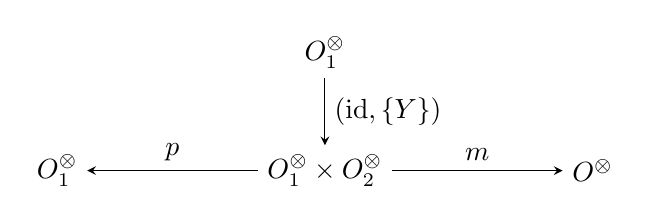
\begin{tikzpicture}[>=stealth,scale=1]
\node (O1) at (0,0) {$O_{1}^{\otimes}$};
\node (P)  at (3.4,0) {$O_{1}^{\otimes}\times O_{2}^{\otimes}$};
\node (O)  at (6.8,0) {$O^{\otimes}$};
\node (T)  at (3.4,1.5) {$O_{1}^{\otimes}$};
\draw[->] (P) -- (O1) node[midway,above] {$p$};
\draw[->] (P) -- (O)  node[midway,above] {$m$};
\draw[->] (T) -- (P)  node[midway,right] {$(\mathrm{id},\{Y\})$};
\end{tikzpicture}
\end{center}
诱导自然函子
\[
\Alg_{O_{2}/O}(\cC)^{\otimes}\to O_{1}^{\otimes}\times_{O^{\otimes}}\cC^{\otimes}.
\]
特别地，我们得到函子
\[
\mathrm{ev}_{Y}\colon\Alg_{O_{2}/O}(\cC)^{\otimes}\to\cC^{\otimes}.
\]
\end{exercise}

\begin{proposition}\label{L26-3.5}（HA.3.2.4.3）
在上述设定下：
\begin{enumerate}[label=(\arabic*),leftmargin=2.4em,itemsep=0.1em]
\item 函子 $\Alg_{O_{2}/O}(\cC)^{\otimes}\to O_{1}^{\otimes}$ 把 $\Alg_{O_{2}/O}(\cC)^{\otimes}$ 展示为 $O_{1}^{\otimes}$ 上的 $\infty$-操作子。此外，$\Alg_{O_{2}/O}(\cC)^{\otimes}$ 中的态射是惰性的，当且仅当
\begin{itemize}[leftmargin=2.2em,itemsep=0.1em]
\item 它在 $O_{1}^{\otimes}$ 中的像是惰性的；
\item 对任意 $Y\in O_{2}$，它在 $\mathrm{ev}_{Y}$ 下的像是惰性的。
\end{itemize}
\item 若 $\cC^{\otimes}\to O^{\otimes}$ 是 $O$-幺半 $\infty$-范畴，则 $\Alg_{O_{2}/O}(\cC)^{\otimes}\to O_{1}^{\otimes}$ 是 $O_{1}$-幺半 $\infty$-范畴。此外，$\Alg_{O_{2}/O}(\cC)^{\otimes}$ 中的态射在 $O_{1}^{\otimes}$ 上是余笛卡尔的，当且仅当对任意 $Y\in O_{2}$，它在 $\mathrm{ev}_{Y}$ 下的像在 $O^{\otimes}$ 上是余笛卡尔的。
\end{enumerate}
\end{proposition}

\begin{example}\label{L26-3.6}
对任意 $\infty$-操作子 $O^{\otimes}$，我们有 $\infty$-操作子映射 $(\mathrm{Comm}\odot O)^{\otimes}\to\mathrm{Comm}^{\otimes}$。由此，对任意 $\infty$-操作子 $\cC^{\otimes}$，存在典范的 $\infty$-操作子 $\Alg_{O}(\cC)^{\otimes}$，它配备到 $\cC^{\otimes}$ 的 $\infty$-操作子映射，且其底层的颜色 $\infty$-范畴是 $\Alg_{O}(\cC)$。此外，若 $\cC$ 是对称幺半的，则 $\Alg_{O}(\cC)$ 也是，且遗忘函子 $\Alg_{O}(\cC)^{\otimes}\to\cC^{\otimes}$ 是对称幺半的。
\end{example}

\begin{exercise}\label{L26-3.7}
在构造~\ref{L26-3.2} 的设定下，当 $O^{\otimes}\coloneqq(O_{1}\odot O_{2})^{\otimes}$ 时，我们有典范等价
\[
\Alg_{O_{1}}(\Alg_{O_{2}}(\cC))\simeq\Alg_{O_{1}\odot O_{2}}(\cC).
\]
\end{exercise}

\begin{proposition}\label{L26-3.8}（HA.3.2.4.7）
设 $\cC^{\otimes}$ 是对称幺半 $\infty$-范畴。则 $\Alg_{\mathrm{Comm}}(\cC)^{\otimes}$ 上的对称幺半结构是余笛卡尔的。特别地，$\Alg_{\mathrm{Comm}}(\cC)$ 承认余积。
\end{proposition}

\begin{remark}\label{L26-3.9}
非形式地说，上述命题说明交换代数的余积由张量积给出。
\end{remark}

\section{$E_{k}$-代数}

\begin{definition}\label{L26-4.1}
设 $k\ge0$ 是非负整数。定义拓扑操作子 ${}^{t}E_{k}^{\otimes}\to\mathrm{Fin}_{*}$，使得：
\begin{itemize}[leftmargin=2.2em,itemsep=0.1em]
\item ${}^{t}E_{k}^{\otimes}$ 中的对象是带标记有限集 $\langle n\rangle$；
\item 从 $\langle m\rangle$ 到 $\langle n\rangle$ 的态射构成的拓扑空间是
\[
\bigsqcup_{\langle m\rangle\xrightarrow{\alpha}\langle n\rangle}\ \prod_{j\in\langle n\rangle^{\circ}}\operatorname{Rect}\bigl(\square^{k}\times\alpha^{-1}(j),\square^{k}\bigr),
\]
其中 $\square\defeq(-1,1)$，而 $\operatorname{Rect}(-,-)$ 是满足下述条件的开嵌入 $\square^{k}\times\alpha^{-1}(j)\to\square^{k}$ 构成的空间：对每个 $i\in\alpha^{-1}(j)$，映射 $f_{i}\colon\square^{k}\to\square^{k}$ 是\textbf{直线嵌入}（rectilinear embedding），即形如
\[
f_{i}(x_{1},\cdots,x_{k})=(a_{1}x_{1}+b_{1},\cdots,a_{k}x_{k}+b_{k})
\]
的映射。
\end{itemize}
令 $E_{k}^{\otimes}$ 为通过函子 $\Cat_{\mathrm{Top}}\to\Cat_{\infty}$ 对应于 ${}^{t}E_{k}^{\otimes}$ 的 $\infty$-操作子。我们称它为 $k$ 维\textbf{小方体 $\infty$-操作子}。
\end{definition}

\begin{exercise}\label{L26-4.2}
$E_{k}^{\otimes}$ 中（活动）$m$ 元运算构成的空间，可以实现为 $\square^{k}$ 中 $m$ 个互异点构成的同伦型。特别地：
\begin{enumerate}[label=(\arabic*),start=0,leftmargin=2.4em,itemsep=0.1em]
\item $E_{k}^{\otimes}$ 是\textbf{带单位的}，即零元运算构成的空间可缩；
\item $E_{k}^{\otimes}$ 是\textbf{约化的}，即一元运算构成的空间可缩；
\item $E_{k}^{\otimes}$ 中二元运算构成的空间同伦于 $S^{k-1}$。
\end{enumerate}
\end{exercise}

\begin{exercise}\label{L26-4.3}
$E_{k}^{\otimes}$ 中（活动）$m$ 元运算构成的空间是 $(k-1)$-连通的，即对 $i<k-1$ 有 $\pi_{i}\simeq0$。
\end{exercise}

\begin{exercise}\label{L26-4.4}
证明上面定义的 $E_{0}^{\otimes}$ 与先前的定义一致：它就是 $\mathrm{Fin}_{*}$ 的由单射态射构成的子范畴。
\end{exercise}

\begin{exercise}\label{L26-4.5}
证明 $E_{1}^{\otimes}\simeq\mathrm{Assoc}^{\otimes}$。
\end{exercise}

\nitem\label{L26-4.6} 对 $0\le k\le k^{\prime}$，我们有 $\infty$-操作子映射 $E_{k}^{\otimes}\to E_{k^{\prime}}^{\otimes}$，它把直线嵌入 $f\colon\square^{k}\to\square^{k}$ 送到 $(f,\id)\colon\square^{k}\times\square^{k^{\prime}-k}\to\square^{k}\times\square^{k^{\prime}-k}$。

\begin{proposition}\label{L26-4.7}（HA.5.1.1.5）
我们有
\[
\colim_{k}E_{k}^{\otimes}\simeq\mathrm{Comm}^{\otimes},
\]
其中余极限在 $\mathrm{Op}_{\infty}$ 中取。特别地，对任意 $\infty$-操作子 $C$，有
\[
\Alg_{\mathrm{Comm}}(C)\simeq\lim_{k}\Alg_{E_{k}}(C).
\]
\end{proposition}

\nitem\label{L26-4.8} 受上述结果启发，我们也记
\[
E_{\infty}^{\otimes}\coloneqq\mathrm{Comm}^{\otimes}.
\]

\begin{construction}\label{L26-4.9}
设 $k,k^{\prime}\ge0$ 是非负整数。我们有函子
\[
{}^{t}E_{k}^{\otimes}\times{}^{t}E_{k^{\prime}}^{\otimes}\to{}^{t}E_{k+k^{\prime}}^{\otimes},
\]
它定义在 $\mathrm{Fin}_{*}\times\mathrm{Fin}_{*}\xrightarrow{\wedge}\mathrm{Fin}_{*}$ 之上，并由 $\square^{k}\times\square^{k^{\prime}}\simeq\square^{k+k^{\prime}}$ 诱导。过渡到 $\infty$-范畴，我们得到函子
\[
E_{k}^{\otimes}\times E_{k^{\prime}}^{\otimes}\to E_{k+k^{\prime}}^{\otimes}.
\]
\end{construction}

\begin{exercise}\label{L26-4.10}
写出上述函子的显式公式，并验证它在每个因子上保持惰性态射。
\end{exercise}

\nitem\label{L26-4.11} 下述结果称为 \textbf{Dunn 加性定理}。

\begin{theorem}\label{L26-4.12}（HA.5.1.2.2）
设 $k,k^{\prime}\ge0$ 是非负整数。函子 $E_{k}^{\otimes}\times E_{k^{\prime}}^{\otimes}\to E_{k+k^{\prime}}^{\otimes}$ 诱导一个等价
\[
(E_{k}\odot E_{k^{\prime}})^{\otimes}\simeq E_{k+k^{\prime}}^{\otimes}.
\]
\end{theorem}

\begin{remark}\label{L26-4.13}
非形式地说，上述定理说明 $E_{k+k^{\prime}}$-代数与「$E_{k^{\prime}}$-代数中的 $E_{k}$-代数」是一样的。
\end{remark}

\begin{corollary}\label{L26-4.14}
设 $k\ge0$ 是非负整数。则 $(E_{k}\odot\mathrm{Comm})^{\otimes}\simeq\mathrm{Comm}^{\otimes}$。
\end{corollary}

\nitem\label{L26-4.15} 下述结果称为 \textbf{Baez--Dolan 稳定化假设}，它由练习~\ref{L26-4.3} 推出。

\begin{proposition}\label{L26-4.16}
设 $\cC$ 是对称幺半 $(n,1)$-范畴。则映射 $E_{k}^{\otimes}\to E_{\infty}^{\otimes}$ 诱导一个等价
\[
\Alg_{E_{\infty}}(\cC)\simeq\Alg_{E_{k}}(\cC),
\]
对任意 $k>n$ 成立。
\end{proposition}

\begin{remark}\label{L26-4.17}
特别地，在普通范畴中，任何超出 $E_{2}$ 的结构都是交换的。
\end{remark}

\nitem\label{L26-4.18} 注意普通范畴自身构成一个 $(2,1)$-范畴。因此，可以存在有趣的、并非对称幺半的 $E_{2}$-幺半普通范畴。

\begin{proposition}\label{L26-4.19}（HA.5.1.2.4）
$E_{2}$-幺半普通范畴恰好就是辫幺半范畴。
\end{proposition}

\begin{remark}\label{L26-4.20}
非形式地说，$E_{2}$ 中二元运算构成的空间同伦于 $S^{1}$，这意味着 $E_{2}$-幺半普通范畴 $\cC$ 给出一个 $\Sigma_{2}$-等变函子 $S^{1}\times\cC\times\cC\to\cC$。对任意点 $s\in S^{1}$，我们得到函子 $\mult_{s}\colon\cC\times\cC\to\cC$ 以及一个等价
\[
\mult_{s}\xrightarrow{\ \simeq\ }\mult_{-s}\circ\sigma,
\]
其中 $\sigma(x,y)\coloneqq(y,x)$。选取从 $1\in S^{1}$ 到 $-1\in S^{1}$ 的一条道路，我们得到等价 $\mult_{1}\xrightarrow{\ \simeq\ }\mult_{-1}$，从而得到等价
\[
\mult_{1}\xrightarrow{\ \simeq\ }\mult_{1}\circ\sigma.
\]
换言之，我们得到函子性同构 $\mult_{1}(x,y)\xrightarrow{\ \simeq\ }\mult_{1}(y,x)$，它们就是相应辫幺半范畴的\textbf{辫态射}。
\end{remark}

\begin{exercise}\label{L26-4.21}
用函子 $S^{1}\times\cC\times\cC\to\cC$ 描述辫的平方。
\end{exercise}

\begin{theorem}\label{L26-4.22}（HA.5.1.1.1）
对 $k\ge1$ 或 $k=\infty$，$\infty$-操作子 $E_{k}^{\otimes}$ 是\textbf{连贯的}。
\end{theorem}

\yizhu{这里的“连贯”是 Lurie 赋予 $\infty$-操作子的一个技术性条件（见 HA.5.1.1.1），与通常所说的“同伦连贯”不是同一概念；译文按 glossary 统一作“连贯”。\textbf{[来源：B]}}

\begin{theorem}\label{L26-4.23}（HA.5.1.3.2）
对 $k\ge1$ 或 $k=\infty$，设 $\cC^{\otimes}\to E_{k}^{\otimes}$ 是与几何实现相容的 $E_{k}$-幺半 $\infty$-范畴。则：
\begin{enumerate}[label=(\arabic*),leftmargin=2.4em,itemsep=0.1em]
\item 对 $A\in\Alg_{/E_{k}}(\cC)$，函子
\[
\Mod^{E_{k}}_{A}(\cC)^{\otimes}\to E_{k}^{\otimes}
\]
是 $E_{k}$-幺半 $\infty$-范畴。
\item 存在典范幺半函子
\[
\Mod^{E_{k}}_{A}(\cC)^{\otimes}\times_{E_{k}^{\otimes}}E_{1}^{\otimes}\to\Mod^{E_{1}}_{A^{\prime}}(\cC\times_{E_{k}}E_{1})^{\otimes},
\]
其中
\[
A^{\prime}\in\Alg_{/E_{1}}(\cC\times_{E_{k}}E_{1})\simeq\Alg^{E_{1}/E_{k}}(\cC)
\]
是复合 $E_{1}^{\otimes}\to E_{k}^{\otimes}\xrightarrow{A}\cC^{\otimes}$。
\end{enumerate}
\end{theorem}

\begin{remark}\label{L26-4.24}
非形式地说，上述定理说明 $E_{k}$-模的相对张量积由底层 $E_{1}$-模的相对张量积给出。
\end{remark}

\appendixsection{因子同调}

\nitem\label{L26-A.1} 给定任意 $E_{k}$-代数 $A$，对任意 $k$-流形 $M$，可以得到一个不变量 $\int_{M}A$，称为 $A$ 在 $M$ 上的\textbf{因子同调}。

\yizhu{“因子同调”（factorization homology）是 Ayala 与 Francis 发展的一种不变量，见本讲参考文献 [AF20]；此处沿用该领域中文文献的译法。\textbf{[来源：A]}}

\nitem\label{L26-A.2} \textbf{建议阅读}\quad HA.5.5.、[AF20]（及其所列参考文献）。

\subsection*{参考文献}
\par\noindent\hangindent=5.2em\hangafter=1 [AF20]\hspace{0.6em}David Ayala and John Francis. A factorization homology primer. In \emph{Handbook of homotopy theory}, pages 39--101. Chapman and Hall/CRC, 2020.
}{}
\IfFileExists{chunks/lec27.tex}{% =============================================================================
%  lec27.tex —— 第 27 讲 E_∞-环（底本 PDF 第 199–203 页）
% =============================================================================
\lecture{27}{$E_\infty$-环}
\begin{center}\small\color{black!55}（底本 PDF 第 199–203 页）\end{center}

本讲解释下述类比：
\begin{center}
\begin{tabular}{ll}
\hline
经典代数 & $\infty$-范畴代数 \\
\hline
集合 & 空间 \\
阿贝尔群 & 谱 \\
张量积 & smash 积 \\
结合环 & $E_{1}$-环 \\
交换环 & $E_{\infty}$-环 \\
\hline
\end{tabular}
\end{center}

\yizhu{本讲的“$E_\infty$-环”即 HA 中的“交换环谱”（commutative ring spectrum）；采用 $E_\infty$ 的说法，是为强调其结构由 $E_\infty$-操作子的代数给出，而不是在 $1$-范畴层面要求严格交换。对照表最后一行把“交换环”对到 $E_\infty$-环，正是这个意思。\textbf{[来源：A]}}

\section{谱与阿贝尔群}

\nitem\label{L27-1.1}
本节解释谱与阿贝尔群之间的类比。

\nitem\label{L27-1.2}
阿贝尔群是 $\Set$ 中的交换幺半群 $G$，且每个元素都有逆。后一条件说的是映射
\[
(p_{1},m)\colon G\times G\to G\times G,\qquad (m,p_{2})\colon G\times G\to G\times G
\]
可逆。此概念在任意笛卡尔对称 monoidal $\infty$-范畴中都有意义。

\begin{definition}\label{L27-1.3}
设 $\cC$ 是承认有限乘积的 $\infty$-范畴。若结合幺半群 $G\in\Mon_{E_1}(\cC)$ 的态射 $(p_{1},m)$ 与 $(m,p_{2})$ 可逆，则称 $G$ 为 $\cC$ 中的\textbf{群}。

对 $1\le k\le\infty$，若 $E_{k}$-幺半群 $G\in\Mon_{E_k}(\cC)$ 在
\[
\Mon_{E_k}(\cC)\to\Mon_{E_1}(\cC)
\]
下的像是一个群，则称 $G$ 为 $\cC$ 中的 \textbf{$E_{k}$-群}\footnote{另一种说法是“群样的 $E_k$-幺半群”（grouplike $E_k$-monoids）。}。令
\[
\Grp_{E_k}(\cC)\subseteq\Mon_{E_k}(\cC)
\]
为 $\cC$ 中 $E_{k}$-群构成的全子 $\infty$-范畴。
\end{definition}

\begin{example}\label{L27-1.4}
设 $X\in\Spc_{*}$ 是任意带基点的空间。对 $0<k<\infty$，$k$ 重环路空间 $\Omega^{k}X$ 带有如下的典范 $E_{k}$-群结构。

选取 $X$ 的一个拓扑实现，则 $\Omega^{k}X$ 可以实现为满足“$f$ 把边界送到 $X$ 的基点”的映射 $f\colon[-1,1]^{k}\to X$ 构成的拓扑空间。对 ${}^{t}E_{k}$ 中的任意 $m$ 元运算 $\gamma\colon\square^{k}\times\langle m\rangle^{\circ}\to\square^{k}$，有同态
\[
\mult_{\gamma}\colon(\Omega^{k}X)^{\times m}\to\Omega^{k}X,
\]
它把 $(f_{1},\dots,f_{m})\in(\Omega^{k}X)^{\times m}$ 送到映射
\[
f(s)\defeq
\begin{cases}
f_{i}(t), & s=\gamma(t,i),\\
*, & \text{其他情形}.
\end{cases}
\]
\end{example}

可以验证，这在 $\Top$ 中定义了 ${}^{t}E_{k}$-群 $\Omega^{k}X$（其中一切都在拓扑空间上充实）。过渡到 $\infty$-范畴，便得到 $\Spc$ 中的 $E_{k}$-群。上述构造对 $X$ 具有函子性，并给出函子
\begin{equation}\label{L27-1.1eq}
\Omega^{k}\colon\Spc_{*}\to\Grp_{E_k}(\Spc).
\end{equation}

\begin{exercise}\label{L27-1.5}
对任意承认有限乘积的 $\infty$-范畴 $\cC$，构造函子 $\Omega^{k}\colon\cC_{*}\to\Grp_{E_k}(\cC)$。提示：Yoneda 引理。
\end{exercise}

\nitem\label{L27-1.6}
函子 \eqref{L27-1.1eq} 不是等价，甚至不是保守的。事实上，$\Omega X$ 只能看见 $X$ 的中性连通分支。结果表明，这正是 \eqref{L27-1.1eq} 不是等价的唯一原因。

\begin{theorem}[Boardman--Vogt--May]\label{L27-1.7}
对 $0<k<\infty$，令 $(\Spc_{*})_{\ge k}\subseteq\Spc_{*}$ 为 $k$-连通空间\footnote{即对 $i<k$ 有 $\pi_{i}\simeq 0$。}构成的全子 $\infty$-范畴。则函子
\begin{equation}\label{L27-1.2eq}
\Omega^{k}\colon(\Spc_{*})_{\ge k}\to\Grp_{E_k}(\Spc)
\end{equation}
是等价。
\end{theorem}

\begin{remark}\label{L27-1.8}
退化情形 $k=0$ 是：$\Spc_{*}\simeq\Mon_{E_0}(\Spc)$。
\end{remark}

\begin{exercise}\label{L27-1.9}
对 $0<k<\infty$，构造典范交换图
\[
\begin{tikzcd}[column sep=4.2em,row sep=3.2em]
(\Spc_{*})_{\ge k+1} \arrow[r,"\Omega"] \arrow[d,"\Omega^{k+1}"] & (\Spc_{*})_{\ge k} \arrow[d,"\Omega^{k}"] \\
\Grp_{E_{k+1}}(\Spc) \arrow[r] & \Grp_{E_k}(\Spc).
\end{tikzcd}
\]
\end{exercise}

\nitem\label{L27-1.10}
由上述练习，可以对 $k$ 取逆向极限，得到连通谱\footnote{即对 $i<0$ 有 $\pi_{i}\simeq 0$。}的下述刻画。

\begin{corollary}\label{L27-1.11}
存在典范等价
\[
\Omega^{\infty}\colon\Sptr_{\ge 0}\xrightarrow{\ \simeq\ }\Grp_{E_\infty}(\Spc),
\]
它与到 $\Spc$ 的遗忘函子相容。
\end{corollary}

\begin{remark}\label{L27-1.12}
换言之，连通谱正是 Picard $\infty$-群胚，即每个对象关于张量积都可逆的对称 monoidal $\infty$-群胚。
\end{remark}

\begin{remark}\label{L27-1.13}
把 \eqref{L27-1.2eq} 的逆记为
\[
B^{k}\colon\Grp_{E_k}(\Spc)\to(\Spc_{*})_{\ge k},
\]
并称之为 \textbf{$k$ 重解环函子}。粗略地说，此函子可如下描述。

对 $k=1$，给定笛卡尔 monoidal $\infty$-范畴 $\cC$ 中的任意结合幺半群 $G$，可以作 Bar 构造
\[
*\times *\rightrightarrows *\times G\times *\rightrightarrows *\times G\times G\times *\cdots,
\]
它是 $\cC$ 中的单纯对象。该图的余极限 $BG$（若存在）计算 $*$ 作为 $G$-双模与自身的相对张量积。可以验证，所得函子
\[
B\colon\Grp_{E_1}(\Spc)\to\Spc_{*}
\]
的像包含在 $(\Spc_{*})_{\ge 0}$ 中，并且确实给出所需的解环函子。

对一般的 $0<k<\infty$，注意复合
\[
\Grp_{E_1}(\Spc)\xrightarrow{\ B\ }(\Spc_{*})_{\ge 1}\to\Spc
\]
与有限乘积交换，因此诱导函子
\[
B\colon\Grp_{E_{k+1}}(\Spc)\simeq\Mon_{E_k}(\Grp_{E_1}(\Spc))\to\Mon_{E_k}(\Spc),
\]
其中第一个等价来自 Dunn 可加性定理。可以验证此函子分解为
\[
B\colon\Grp_{E_{k+1}}(\Spc)\to\Grp_{E_k}(\Spc).
\]
于是得到函子
\[
B^{k}\colon\Grp_{E_k}(\Spc)\to\Spc_{*}.
\]
可以验证其像包含在 $(\Spc_{*})_{\ge k}$ 中，并且确实给出所需的 $k$ 重解环函子。
\end{remark}

\section{smash 积与张量积}

\nitem\label{L27-2.1}
本节解释谱的 smash 积与阿贝尔群的张量积之间的类比。

\nitem\label{L27-2.2}
回忆有函子
\[
\pi_{\bullet}\colon\Sptr\to\mathrm{grAb},
\]
它把谱 $X$ 送到其同伦群
\[
\pi_{m}X\simeq\pi_{0}\Map_{\Sptr}(S[m],X).
\]

\begin{construction}\label{L27-2.3}
考虑 $\Sptr$ 中由单位结构给出的同构 $S\otimes S\xrightarrow{\ \simeq\ }S$。利用 $-\otimes-$ 与每个因子的余极限交换这一事实，对整数 $m,n$ 得到同构
\[
S[m]\otimes S[n]\xrightarrow{\ \simeq\ }S[m+n].
\]
因此对谱 $X,Y$，得到空间之间的态射
\[
\Map_{\Sptr}(S[m],X)\times\Map_{\Sptr}(S[n],Y)\to\Map_{\Sptr}(S[m]\otimes S[n],X\otimes Y)
\xrightarrow{\ \simeq\ }\Map_{\Sptr}(S[m+n],X\otimes Y).
\]
取 $\pi_{0}$，得到映射
\[
\pi_{m}X\times\pi_{n}Y\to\pi_{m+n}(X\otimes Y).
\]
可以验证此映射双线性，因此给出 $\Ab$ 中的态射
\[
\pi_{m}X\otimes\pi_{n}Y\to\pi_{m+n}(X\otimes Y),
\]
它们可以组装为态射
\[
\pi_{\bullet}X\otimes\pi_{\bullet}Y\to\pi_{\bullet}(X\otimes Y),
\]
其中源为分次张量积。可以验证，这给出函子 $\pi_{\bullet}$ 上的右 lax 对称 monoidal 结构\footnote{此结构中没有更高阶数据，因为 $\mathrm{grAb}$ 是通常范畴。}。换言之，有 $\infty$-操作子映射
\[
\pi_{\bullet}\colon\Sptr^{\otimes}\to\mathrm{grAb}^{\otimes}.
\]
\end{construction}

\begin{warning}\label{L27-2.4}
函子 $\pi_{\bullet}$ 不是对称 monoidal 的。事实上，$\pi_{\bullet}(S)$ 与 $\Z$ 大不相同。
\end{warning}

\nitem\label{L27-2.5}
下述练习说明，限制到 $\Sptr_{\ge 0}$ 时 $\pi_{0}$ 是对称 monoidal 的。

\begin{exercise}\label{L27-2.6}
全子 $\infty$-范畴 $\Sptr_{\ge 0}\subseteq\Sptr$ 对 smash 积封闭。提示：$\Sptr_{\ge 0}$ 由 $S$ 在余极限与扩张下生成。
\end{exercise}

\begin{exercise}\label{L27-2.7}
$\pi_{0}\colon\Sptr_{\ge 0}\to\Ab$ 上的 lax 对称 monoidal 结构是严格的。
\end{exercise}

\begin{exercise}\label{L27-2.8}
用相应的 Picard $\infty$-群胚描述谱的 smash 积。提示：可以先看 $E_{0}$ 情形。
\end{exercise}

\section{$E_{k}$-环}

\begin{definition}\label{L27-3.1}
给 $\Sptr$ 装备 smash 积对称 monoidal 结构。对 $0\le k\le\infty$，\textbf{$E_{k}$-环}是 $\Sptr$ 中的 $E_{k}$-代数。
\end{definition}

\begin{construction}\label{L27-3.2}
由于 $\Sptr\to\mathrm{grAb}$ 自然右 lax 对称 monoidal，得到函子
\[
\Alg_{E_k}(\Sptr)\to\Alg_{E_k}(\mathrm{grAb}).
\]
因此：
\begin{itemize}[leftmargin=2.2em,itemsep=0.1em]
\item 对 $E_{1}$-环 $A$，得到结合环 $\pi_{\bullet}A$；
\item 对 $k\ge 2$ 的 $E_{k}$-环 $A$，得到分次交换环 $\pi_{\bullet}A$。
\end{itemize}
\end{construction}

\begin{construction}\label{L27-3.3}
注意 $\pi_{0}\colon\Sptr_{\ge 0}\to\Ab$ 可以通过 $\Ab\simeq\Sptr^{\heartsuit}$ 等同于函子 $\tau_{\le 0}$，并且它有右伴随
\[
\Ab\to\Sptr_{\ge 0},\qquad R\mapsto HR,
\]
把 $R$ 送到 Eilenberg--MacLane 谱 $HR$。由于左伴随函子自然对称 monoidal，右伴随带有右 lax 对称 monoidal 结构。特别地，得到函子
\[
\Alg_{E_k}(\Ab)\to\Alg_{E_k}(\Sptr_{\ge 0})\to\Alg_{E_k}(\Sptr).
\]
换言之：
\begin{itemize}[leftmargin=2.2em,itemsep=0.1em]
\item 对结合环 $R$，得到 $HR$ 上的 $E_{1}$-环结构；
\item 对交换环 $R$，得到 $HR$ 上的 $E_{\infty}$-环结构。
\end{itemize}
\end{construction}

\nitem\label{L27-3.4}
最后一项任务是把 $HR$-模与 $R$-模联系起来。为简便起见，我们在 $E_{\infty}$ 情形下工作。

从现在起，设 $R$ 是交换环，$\Mod_{R}$ 是 $R$-模范畴（阿贝尔范畴），$\Mod_{HR}(\Sptr)$ 是 $\Sptr$ 中 $HR$-模的 $\infty$-范畴。

\begin{construction}\label{L27-3.5}
考虑 $\Mod_{R}$ 上的相对张量积对称 monoidal 结构。过渡到导出 $\infty$-范畴，得到 $D(R)\defeq D(\Mod_{R})$ 上的可表现对称 monoidal 结构（细节见 HA.7.1.2.12）。由于 $D(R)$ 稳定，得到交换代数对象 $D(R)\in\Alg_{\mathrm{Comm}}(\PrSt^{L})$。回忆 $\Sptr$ 是 $\PrSt^{L}$ 的单位。于是得到 $\Alg_{\mathrm{Comm}}(\PrSt^{L})$ 中的态射 $\Sptr\to D(R)$。换言之，一个对称 monoidal 函子
\[
F\colon\Sptr\to D(R).
\]
\end{construction}

\nitem\label{L27-3.6}
注意底函子 $\Sptr\to D(R)$ 是唯一的保余极限函子，它把 $S\in\Sptr$ 送到 $R\in D(R)$。另一方面，复合
\[
G\colon D(R)\to D(\Z)\xrightarrow{\ DK\ }\Sptr
\]
的左伴随也把 $S$ 送到 $R$。于是得到伴随
\[
F\colon\Sptr\rightleftarrows D(R)\colon G,
\]
其中 $F$ 对称 monoidal，而 $G$ 右 lax 对称 monoidal\footnote{更确切地说，我们有在 $\mathrm{Fin}_{*}$ 上定义的伴随 $\Sptr^{\otimes}\rightleftarrows D(R)^{\otimes}$。}。注意 $G$ 也保持余极限。

\begin{exercise}\label{L27-3.7}
证明复合
\[
G\circ F\colon\Sptr\to D(R)\to\Sptr
\]
等同于 $HR\otimes-$。
\end{exercise}

\begin{theorem}[HA.7.1.2.13]\label{L27-3.8}
存在对称 monoidal $\infty$-范畴的典范等价
\[
\Mod_{HR}(\Sptr)\simeq D(R),
\]
使得伴随 $F\colon\Sptr\rightleftarrows D(R)\colon G$ 可以等同于沿单位态射 $u\colon S\to HR$ 的
\[
\ind_{u}\colon\Mod_{S}(\Sptr)\rightleftarrows\Mod_{HR}(\Sptr)\colon\res_{u}.
\]
\end{theorem}

\appendixsection{Barr--Beck--Lurie 定理}

\yizhu{“$G$-分裂单纯余极限”指：对单纯对象 $V\in\cD_{\Delta}$，若 $G(V)$ 在 $\cC$ 中带有分裂（即其面/退化结构额外给出收缩），则 $V$ 在 $\cD$ 中有余极限，且 $G$ 保持该余极限。这是 HA.4.7.5.3 所用“Beck 条件”的 $\infty$-版本，替代了经典 Barr--Beck 定理中“$G$ 反射等化子”的要求。\textbf{[来源：A]}}

\nitem\label{L27-A.1}
定理 \ref{L27-3.8} 的证明的关键输入是下述定理。

\begin{theorem}[Barr--Beck--Lurie]\label{L27-A.2}
设 $F\colon\cC\rightleftarrows\cD\colon G$ 是 $\infty$-范畴之间的伴随，且满足
\begin{enumerate}[label=(\roman*),leftmargin=2.4em,itemsep=0.1em]
\item 函子 $G$ 保守；
\item 函子 $G$ 保持 $G$-分裂单纯余极限\footnote{这指的是：设 $V\in\cD_{\Delta}\defeq\Fun(\Delta^{\op},\cD)$ 是使得 $G(V)$ 承认分裂的单纯对象。则 $V$ 在 $\cD$ 中承认余极限，且该余极限被 $G$ 保持。}。
\end{enumerate}
则存在典范等价 $\cD\simeq\mathrm{LMod}_{T}(\cC)$，其中 $T$ 是作用在 $\cC$ 上的单子，其底自同态为 $G\circ F$。此外，伴随 $F\colon\cC\rightleftarrows\cD\colon G$ 可以等同于
\[
\ind_{T}\colon\cC\to\mathrm{LMod}_{T}(\cC)\colon\oblv_{T}.
\]
\end{theorem}

\nitem\label{L27-A.3}
\textbf{建议阅读}\quad HA.4.7。
}{}

\end{document}
